% Options for packages loaded elsewhere
\PassOptionsToPackage{unicode}{hyperref}
\PassOptionsToPackage{hyphens}{url}
%
\documentclass[
]{book}
\usepackage{lmodern}
\usepackage{amsmath}
\usepackage{ifxetex,ifluatex}
\ifnum 0\ifxetex 1\fi\ifluatex 1\fi=0 % if pdftex
  \usepackage[T1]{fontenc}
  \usepackage[utf8]{inputenc}
  \usepackage{textcomp} % provide euro and other symbols
  \usepackage{amssymb}
\else % if luatex or xetex
  \usepackage{unicode-math}
  \defaultfontfeatures{Scale=MatchLowercase}
  \defaultfontfeatures[\rmfamily]{Ligatures=TeX,Scale=1}
\fi
% Use upquote if available, for straight quotes in verbatim environments
\IfFileExists{upquote.sty}{\usepackage{upquote}}{}
\IfFileExists{microtype.sty}{% use microtype if available
  \usepackage[]{microtype}
  \UseMicrotypeSet[protrusion]{basicmath} % disable protrusion for tt fonts
}{}
\makeatletter
\@ifundefined{KOMAClassName}{% if non-KOMA class
  \IfFileExists{parskip.sty}{%
    \usepackage{parskip}
  }{% else
    \setlength{\parindent}{0pt}
    \setlength{\parskip}{6pt plus 2pt minus 1pt}}
}{% if KOMA class
  \KOMAoptions{parskip=half}}
\makeatother
\usepackage{xcolor}
\IfFileExists{xurl.sty}{\usepackage{xurl}}{} % add URL line breaks if available
\IfFileExists{bookmark.sty}{\usepackage{bookmark}}{\usepackage{hyperref}}
\hypersetup{
  pdftitle={Data analysis using R for Psychology and Social Science},
  pdfauthor={Alexander (Sasha) Pastukhov},
  hidelinks,
  pdfcreator={LaTeX via pandoc}}
\urlstyle{same} % disable monospaced font for URLs
\usepackage{color}
\usepackage{fancyvrb}
\newcommand{\VerbBar}{|}
\newcommand{\VERB}{\Verb[commandchars=\\\{\}]}
\DefineVerbatimEnvironment{Highlighting}{Verbatim}{commandchars=\\\{\}}
% Add ',fontsize=\small' for more characters per line
\usepackage{framed}
\definecolor{shadecolor}{RGB}{248,248,248}
\newenvironment{Shaded}{\begin{snugshade}}{\end{snugshade}}
\newcommand{\AlertTok}[1]{\textcolor[rgb]{0.94,0.16,0.16}{#1}}
\newcommand{\AnnotationTok}[1]{\textcolor[rgb]{0.56,0.35,0.01}{\textbf{\textit{#1}}}}
\newcommand{\AttributeTok}[1]{\textcolor[rgb]{0.77,0.63,0.00}{#1}}
\newcommand{\BaseNTok}[1]{\textcolor[rgb]{0.00,0.00,0.81}{#1}}
\newcommand{\BuiltInTok}[1]{#1}
\newcommand{\CharTok}[1]{\textcolor[rgb]{0.31,0.60,0.02}{#1}}
\newcommand{\CommentTok}[1]{\textcolor[rgb]{0.56,0.35,0.01}{\textit{#1}}}
\newcommand{\CommentVarTok}[1]{\textcolor[rgb]{0.56,0.35,0.01}{\textbf{\textit{#1}}}}
\newcommand{\ConstantTok}[1]{\textcolor[rgb]{0.00,0.00,0.00}{#1}}
\newcommand{\ControlFlowTok}[1]{\textcolor[rgb]{0.13,0.29,0.53}{\textbf{#1}}}
\newcommand{\DataTypeTok}[1]{\textcolor[rgb]{0.13,0.29,0.53}{#1}}
\newcommand{\DecValTok}[1]{\textcolor[rgb]{0.00,0.00,0.81}{#1}}
\newcommand{\DocumentationTok}[1]{\textcolor[rgb]{0.56,0.35,0.01}{\textbf{\textit{#1}}}}
\newcommand{\ErrorTok}[1]{\textcolor[rgb]{0.64,0.00,0.00}{\textbf{#1}}}
\newcommand{\ExtensionTok}[1]{#1}
\newcommand{\FloatTok}[1]{\textcolor[rgb]{0.00,0.00,0.81}{#1}}
\newcommand{\FunctionTok}[1]{\textcolor[rgb]{0.00,0.00,0.00}{#1}}
\newcommand{\ImportTok}[1]{#1}
\newcommand{\InformationTok}[1]{\textcolor[rgb]{0.56,0.35,0.01}{\textbf{\textit{#1}}}}
\newcommand{\KeywordTok}[1]{\textcolor[rgb]{0.13,0.29,0.53}{\textbf{#1}}}
\newcommand{\NormalTok}[1]{#1}
\newcommand{\OperatorTok}[1]{\textcolor[rgb]{0.81,0.36,0.00}{\textbf{#1}}}
\newcommand{\OtherTok}[1]{\textcolor[rgb]{0.56,0.35,0.01}{#1}}
\newcommand{\PreprocessorTok}[1]{\textcolor[rgb]{0.56,0.35,0.01}{\textit{#1}}}
\newcommand{\RegionMarkerTok}[1]{#1}
\newcommand{\SpecialCharTok}[1]{\textcolor[rgb]{0.00,0.00,0.00}{#1}}
\newcommand{\SpecialStringTok}[1]{\textcolor[rgb]{0.31,0.60,0.02}{#1}}
\newcommand{\StringTok}[1]{\textcolor[rgb]{0.31,0.60,0.02}{#1}}
\newcommand{\VariableTok}[1]{\textcolor[rgb]{0.00,0.00,0.00}{#1}}
\newcommand{\VerbatimStringTok}[1]{\textcolor[rgb]{0.31,0.60,0.02}{#1}}
\newcommand{\WarningTok}[1]{\textcolor[rgb]{0.56,0.35,0.01}{\textbf{\textit{#1}}}}
\usepackage{longtable,booktabs}
% Correct order of tables after \paragraph or \subparagraph
\usepackage{etoolbox}
\makeatletter
\patchcmd\longtable{\par}{\if@noskipsec\mbox{}\fi\par}{}{}
\makeatother
% Allow footnotes in longtable head/foot
\IfFileExists{footnotehyper.sty}{\usepackage{footnotehyper}}{\usepackage{footnote}}
\makesavenoteenv{longtable}
\usepackage{graphicx}
\makeatletter
\def\maxwidth{\ifdim\Gin@nat@width>\linewidth\linewidth\else\Gin@nat@width\fi}
\def\maxheight{\ifdim\Gin@nat@height>\textheight\textheight\else\Gin@nat@height\fi}
\makeatother
% Scale images if necessary, so that they will not overflow the page
% margins by default, and it is still possible to overwrite the defaults
% using explicit options in \includegraphics[width, height, ...]{}
\setkeys{Gin}{width=\maxwidth,height=\maxheight,keepaspectratio}
% Set default figure placement to htbp
\makeatletter
\def\fps@figure{htbp}
\makeatother
\setlength{\emergencystretch}{3em} % prevent overfull lines
\providecommand{\tightlist}{%
  \setlength{\itemsep}{0pt}\setlength{\parskip}{0pt}}
\setcounter{secnumdepth}{5}
\usepackage{booktabs}
\usepackage{booktabs}
\usepackage{longtable}
\usepackage{array}
\usepackage{multirow}
\usepackage{wrapfig}
\usepackage{float}
\usepackage{colortbl}
\usepackage{pdflscape}
\usepackage{tabu}
\usepackage{threeparttable}
\usepackage{threeparttablex}
\usepackage[normalem]{ulem}
\usepackage{makecell}
\usepackage{xcolor}
\ifluatex
  \usepackage{selnolig}  % disable illegal ligatures
\fi
\usepackage[]{natbib}
\bibliographystyle{apalike}

\title{Data analysis using R for Psychology and Social Science}
\author{Alexander (Sasha) Pastukhov}
\date{2021-11-30}

\begin{document}
\maketitle

{
\setcounter{tocdepth}{1}
\tableofcontents
}
\hypertarget{introduction}{%
\chapter*{Introduction}\label{introduction}}
\addcontentsline{toc}{chapter}{Introduction}

This book will (try to) teach you how to perform typical data analysis tasks: reading data, transforming and cleaning it up so you can visualize it and perform a statistical analysis of your choice. It covers most topics that you need to get you started but it cannot cover them all. One advantage of R is a sheer size of its ecosystem with new incredible libraries appearing very much on a daily basis. Covering them all is beyond the scope of any book, so instead I will concentrate on (trying to) building a solid understanding of things that you need to extend your R knowledge. Because of that some early chapters (e.g., on \protect\hyperlink{vectors}{vectors}, \protect\hyperlink{tables}{tables}, or \protect\hyperlink{ux5cux23functions}{functions}) might feel boring and too technical making you wonder why didn't we start with some exciting and useful analysis, working our way down to finer details. I have tried that\footnote{As a matter of fact, this was my approach when learning R.} but, unfortunately, philosophy of R is about have many almost identical ways of achieving the same end. If you do not learn these finer details, you waste time wondering why seemingly the same code works in one case but fails in mysterious ways in the other one\footnote{Talking from a personal experience here.}. Therefore, please bear with me and struggle through vectors (which are everywhere), oddities and inconsistencies of subsetting, and learning how to write a function before you even started to use them properly. I can only promise that, from my personal experience, this is definitely worth the effort.

An important note: this book will \emph{not} teach you statistics or machine learning. I will mention some widely used packages and functions for performing statistical analysis but I will not go into the details of how they work or how to interpret their output. If you know (enough of) statistics, you will have little trouble understanding how to work with these packages and functions. If you do not, no amount of reading of manuals will make it clearer.

\hypertarget{why-r}{%
\section*{Why R?}\label{why-r}}
\addcontentsline{toc}{section}{Why R?}

There are many software tools that allow you preprocess, plot, and analyze your data. Some cost money (SPSS, Matlab), some are free just like R (Python, Julia). Moreover, you can replicate all analysis that we will perform using Python in combination with \href{https://jupyter.org/}{Jupyter notebooks} (for reproducible analysis), \href{https://pandas.pydata.org/}{Pandas} (for Excel-style table), and \href{https://www.statsmodels.org/stable/index.html}{statmodels} (for statistical analysis). R is hardly perfect. For example, its subsetting system is confusing and appears to follow ``convenience over safety'' approach that does not sit particularly well with me. However, R in combination with piping and \href{https://www.tidyverse.org/}{Tidyverse} family of packages makes it incredibly easy to write simple, powerful and expressive code, which is very easy to understand (a huge plus, as you will discover). I will run circles around myself trying to replicate the same analysis in Python or Matlab. In addition, R is loved by mathematicians and statisticians, so it tends to have implementations for all cutting edge methods (my impression is that even Python is lagging behind it in that respect).

\hypertarget{why-tidyverse}{%
\section*{Why Tidyverse}\label{why-tidyverse}}
\addcontentsline{toc}{section}{Why Tidyverse}

The material is heavily skewed towards using \href{https://www.tidyverse.org/}{Tidyverse} family of packages. It looks different enough from base R to the point that one might call it a ``dialect'' of R\footnote{R is extremely flexible, making it possible to redefine its own syntax.}. Learning Tidyverse means that you have twice as many things to learn: I will always introduce both base R and Tidyverse version. \href{https://www.tidyverse.org/}{Tidyverse} is the main reason I use R (rather than Python or Julia) as it makes data analysis a breeze and makes your life so much easier. This is why I want you to learn its ways. At the same time, there is plenty of useful code that uses base R, so you need to know and understand it as well.

As a matter of fact, R is so rich and flexible that there many dialects and, therefore, plenty of opinion differences \footnote{Just ask about ``base R vs.~Tidyverse'' on Twitter and see the thread set itself on fire}. For example, \href{https://github.com/Rdatatable/data.table}{data.table} package re-implements the same functionality as base R and Tidyverse in very compact way. I does not fit my style but it might be something that feels natural to you. There are also other packages to handle things like layout out your figures or working with summary tables that might suit you better. Point is, these material barely scratches the surfaces in terms of tools and approaches that you can use. View it as a starting point for your exploration not the complete map.

Another thing to keep in mind is that Tidyverse is under very active development. This means that parts of this material could be outdated by the time you read it. E.g., \emph{dplyr} \href{https://dplyr.tidyverse.org/reference/do.html}{do()} verb was superseded by an overpowered \href{https://dplyr.tidyverse.org/reference/summarise.html}{summarise()} function, a warning generated by \href{https://readr.tidyverse.org/}{readr} package was adapted for humans but now require an extra step to be used for column specification, etc. None of the changes are breaking and deprecation process is deliberately slow (e.g., \href{https://dplyr.tidyverse.org/reference/do.html}{do()} still works), so even when outdated the code in the book should still work for quite some time. However, you should keep in mind that things \emph{might} have changed, so it is a good idea to check an official manual from time to time.

\hypertarget{about-the-seminar}{%
\section*{About the seminar}\label{about-the-seminar}}
\addcontentsline{toc}{section}{About the seminar}

This is a material for \emph{Applied data analysis for psychology using the open-source software R} seminar as taught at \href{https://www.uni-bamberg.de/psychologie/}{Institute of Psychology} at University of Bamberg. Each chapter covers a single seminar, introducing necessary ideas and is accompanied by a notebook with exercises, which you need to complete and submit. To pass the seminar, you will need to complete all assignments. You do not need to complete or provide correct solutions for \emph{all} the exercises to pass the course and information on how the points for exercises will be converted to an actual grade (if you need one) or ``pass'' will be available during the seminar.

The material assumes no foreknowledge of R or programming in general from a reader. Its purpose is to gradually build up your knowledge and introduce to a typical analysis pipeline. It is based on a data that is typical for the field (repeated measures, appearance, accuracy and response time measurements, Likert scale reports, etc.) and you are welcome to suggest your own data set for analysis. Even if you already performed the analysis using some other program, it would still be insightful to compare the different ways and, perhaps, you might gain a new insight. Plus, it is more engaging to work on your data.

Remember that throughout the seminar you can and should(!) always ask me whenever something is unclear, you do not understand a concept or logic behind certain code, or you simply got stuck. Do not hesitate to write me in the team or (better) directly to me in the chat (in the latter case, the notifications are harder miss and we don't spam others with our conversation).

\hypertarget{thinking-like-a-computer}{%
\section*{Thinking like a computer}\label{thinking-like-a-computer}}
\addcontentsline{toc}{section}{Thinking like a computer}

In some exercises your will not be writing code but reading and understanding it. Your job in this case is ``to think like a computer''. Your advantage is that computers are very dumb, so instructions for them must be written in a very simple, clear, and unambiguous way. This means that, with practice, reading code is easy for a human (well, reading a well-written code is easy, you will eventually encounter ``spaghetti-code'' which is easier to rewrite from scratch than to understand). In each case, you simply go through the code line-by-line, doing all computations by hand and writing down values stored in the variables (if there are too many to keep track of). Once you go through the code in this manner, it should be completely transparent for you. No mysteries should remain, you should have no doubts or uncertainty about any(!) line. Moreover, you then can run the code and check that the values you are getting from computer match yours. Any difference means you made a mistake and code is working differently from how you think it does. In any case, \textbf{if you not 100\% sure about any line of code, ask me, so we can go through it together!}

In a sense, this is the most important programming skill. It is impossible to learn how to write, if you cannot read the code first! Moreover, when programming you will probably spend more time reading the code and making sure that it works correctly than writing the new code. Thus, use this opportunity to practice and never use the code that you do not understand completely. Thus, there is nothing wrong in using \href{https://stackoverflow.com/}{stackoverflow} but \textbf{never} use the code you do not understand (do not blindly copy-paste)!

\hypertarget{about-the-material}{%
\section*{About the material}\label{about-the-material}}
\addcontentsline{toc}{section}{About the material}

The material is \textbf{free to use} and is licensed under the \href{https://creativecommons.org/licenses/by-nc-nd/4.0/}{Creative Commons Attribution-NonCommercial-NoDerivatives V4.0 International License}.

\hypertarget{software}{%
\chapter*{Software}\label{software}}
\addcontentsline{toc}{chapter}{Software}

\hypertarget{install-r}{%
\section{Installing R}\label{install-r}}

Go to \href{https://cloud.r-project.org/}{r-project.org} and download a current stable version of R for your platform. Run the installer, accepting all defaults. The installer will ask you whether you also want a 32-bit version to be installed alongside 64-bit. You probably won't need 32-bit, so if space is at premium you can skip it. Otherwise, it will make very little difference.

\hypertarget{install-rstudio}{%
\section{Installing R-Studio}\label{install-rstudio}}

Go to \href{https://rstudio.com/products/rstudio/download/}{rstudio.com} and download \emph{RStudio Desktop Free} edition for your platform. Install it using defaults. The \emph{R-Studio} is an integrated development environment for R but you need to install R separately first! The R-Studio will automatically detect latest R that you have and, in case you have several versions of R installed, you will be able to alter that choice via \emph{Tools / Global Options\ldots{}} menu.

I will explain the necessary details on using R-Studio throughout the seminar but the \href{https://github.com/rstudio/cheatsheets/raw/master/rstudio-ide.pdf}{official cheatsheet} is an excellent, compact, and up-to-date source of information. In fact, R Studio has numerous \href{https://rstudio.com/resources/cheatsheets/}{cheatsheets} that describe individual packages in a compact form.

\hypertarget{install-rtools}{%
\section{Installing RTools}\label{install-rtools}}

If you are using Windows, you might need \href{https://cran.r-project.org/bin/windows/Rtools/}{Rtools} for building and running some packages. You do not need to install it at the beginning, but when we will need it later, just following the link above, download the latest \emph{Rtools} version, run the installer using the defaults and follow the instructions on that page to put Rtools on the PATH!

\hypertarget{install.packages}{%
\section*{Installing packages}\label{install.packages}}
\addcontentsline{toc}{section}{Installing packages}

The real power of R lies in a vast community-driven family of packages suitable for any occasion. The default repository used by R and R-Studio is \href{https://cran.r-project.org/}{The Comprehensive R Archive Network} (a.k.a. \emph{CRAN}). It has very strict requirements for submitted packages, which makes it very annoying for the authors but ensures high quality for you. We will use CRAN as a sole source of packages, but there are alternatives, such as \href{http://www.bioconductor.org/}{Bioconductor} that might have a package that is missing at CRAN. The Bioconductor relies on its own package manager, so you will need to consult the latest manual on their website.

To install a CRAN package you have two alternatives: via command line function or via R-Studio package manager interface (which will call the function for you). In the former case, go to \emph{Console} tab and type \texttt{install.packages("package-name")}, for example \texttt{install.packages("tidyverse")}, and press \textbf{Enter}.

\begin{center}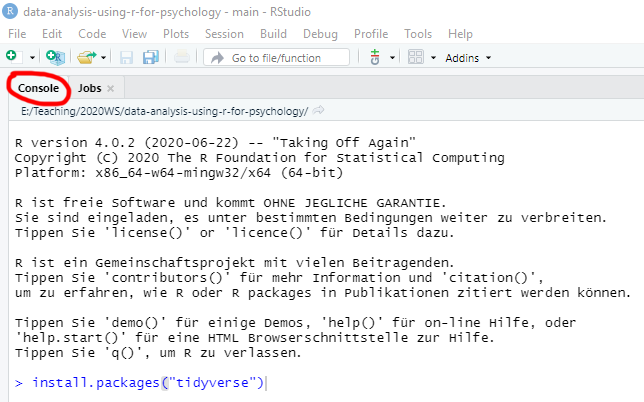
\includegraphics[width=1\linewidth]{images/install-packages-cmd} \end{center}

Alternatively, go to \emph{Packages} tab, click on \emph{Install} button, enter a package name in the window (it has autocomplete to help you), and press \emph{Install}.

\begin{center}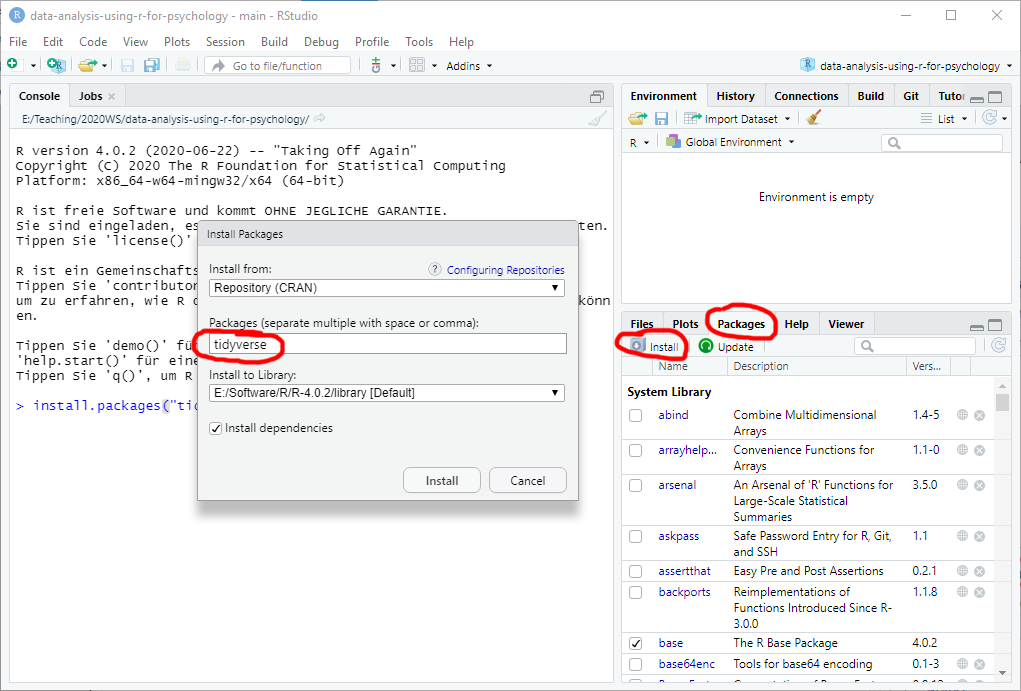
\includegraphics[width=1\linewidth]{images/install-packages-gui} \end{center}

Sometimes, R will ask whether you want to install packages from source. In this case, it will grab the source code and compile the package, which takes time and requires \protect\hyperlink{install-rtools}{RTools}. In most cases, you can say ``No'' to install a pre-build binary version. The binary version will be slightly outdated but the emphasis is on \emph{slightly}.

On other occasions, R-Studio will suggest restarting R Session as packages that need to be updated in use. You can do that but, in my experience, this could a repetetive experience if one of the packages is used R Studio itself (so it starts it in a new session, realizes that it is in use, suggests to restart the session, etc.) My solution is to close \emph{all} R Studio windows and use R directly. For Windows, you can find it the Start Menu, just make sure that you are using the correct version (also make sure it is \emph{x64}). Then, I use \texttt{install.packages()} to install and update everything I need.

\hypertarget{minimal-set-of-packages}{%
\section{Minimal set of packages}\label{minimal-set-of-packages}}

Please install the following packages:

\begin{itemize}
\tightlist
\item
  \texttt{tidyverse} : includes packages from data creation (\texttt{tibble}), reading (\texttt{readr}), wrangling (\texttt{dplyr}, \texttt{tidyr}), plotting (\texttt{ggplot2}). Plus type specific packages (\texttt{stringr} for strings, \texttt{forcats} for factors) and functional programming (\texttt{purrr}).
\item
  \texttt{rmarkdown} : package for working with RMarkdown notebooks, which will we use to create reproducible analysis.
\item
  \texttt{fs} : file system utilities.
\end{itemize}

\hypertarget{installr}{%
\section{Keeping R and packages up-to-date}\label{installr}}

R and packages are getting constantly improved, so it is a good idea to regularly update them. For packages, you can use \emph{Tools / Check for Packages Updates\ldots{}} menu in R-Studio. To update R and, optionally, packages, you can use \href{https://www.r-project.org/nosvn/pandoc/installr.html}{installr} package that can install newest R (but it keeps old version!) optionally copying your entire library of packages, updating packages, etc. It is easy to use even in R itself, as it creates an extra menu to make your life easier. For R-Studio itself, use \emph{Help / Check for Updates} menu and install a newer version, if it is available (it is generally a good idea to keep your R-Studio in the newest state).

\hypertarget{reproducable-research}{%
\chapter{Reproducable Research: Projects and RMarkdown Notebooks}\label{reproducable-research}}

Our aim is to create reproducible research and analysis. It is a crucial component of the open science movement but is even more important for your own research or study projects. You want to create a self-contained well-documented easy-to-understand reproducible analysis. A complete self-sufficient code that others and, most importantly, future-you can easily understand saves you time and gives you a deeper insight into the results (less mystery is better in cases like these). It also makes it easier to communicate your results to other researchers or fellow students.

You should also \emph{always} consider posting your results and analysis online at public repositories such as \href{https://osf.io/}{OSF}, \href{https://www.scidb.cn/en}{Science Data Bank}, or \href{https://github.com/}{GitHub}. This not only help others but forces you into making such data + analysis archive more thoroughly. That, in turns, makes it easier for future-you to return to the data and the analysis.

\hypertarget{projects}{%
\section{Projects}\label{projects}}

One of the most annoying features of R is that looks for files and folders only relative to its ``working directory'', which is set via \href{https://www.rdocumentation.org/packages/base/versions/3.6.2/topics/getwd}{setwd(dir)} function. What makes it particularly confusing is that your currently open file may be in some \emph{other} folder. If you simply use \emph{File / Open}, navigate to that file and open it, it does not change your working directory. Similarly, in R-Studio you can navigate through file system using \emph{Files} tab and open some folder you are interested in but that \textbf{does not make it a working directory}. You need to click on \emph{More} and \emph{Set As Working Directory} to make this work (that trick won't work for an opened file).

\begin{center}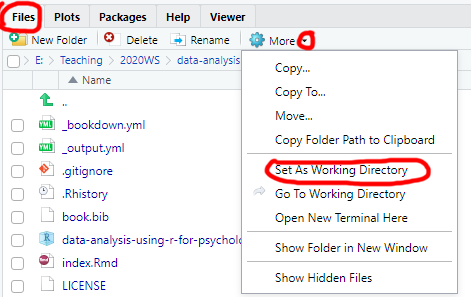
\includegraphics[width=1\linewidth]{images/setwd-gui} \end{center}

In short, it may \emph{look} that you are working in a particular folder but R will have its own opinion about this. Whenever this happens, it is really confusing and involves a lot of cursing as R cannot find files that you can clearly see with your own eyes. To avoid this you should organize any program, project or seminar as an \emph{R Project}, which assumes that all necessary files are in the project folder, which is also the working directory. R Studio has some nice project-based touches as well, like keeping tracking of which files you have open, providing version control, etc. Bottom line, \textbf{always} create a new R-project to organize yourself, even if it involves just a single file to try something out. Remember, ``Nothing is more permanent than a temporary solution!'' Which is why you should \textbf{always} write your code, as if it is for a long term project (good style, comprehensible variable names, comments, etc.), otherwise your temporary solution grows into permanent incomprehensible spaghetti code.

Let us create a new project for this seminar. Use \emph{File / New Project\ldots{}}, which will give you options of creating it in a new directory (you get to come up with a name), using an existing directory (project will be named after that directory), or check it out from remote repository (something we won't talk about just yet). You can do it either way. This will be a project folder for this seminar and you will need to put all notebooks and external data files into that folder. Next time you need to open it, you can use \emph{File / Recent Projects} menu, \emph{File / Open Project\ldots{}}\texttt{\_\ menu,\ or\ simply\ open\ the}.Rproj` file in that folder.

\hypertarget{rmarkdown}{%
\section{RMarkdown}\label{rmarkdown}}

\href{https://rmarkdown.rstudio.com/}{RMarkdown notebooks} combine formatted text, figures, references (via \href{http://www.bibtex.org/}{bibtex}) and cross-references with code\footnote{This material was prepared using RMarkdown, \href{(https://yihui.org/knitr/)}{knitr}, and \href{https://bookdown.org/}{bookdown}}. When a notebook is \href{https://yihui.org/knitr/}{knitted}, all the code is ran and its output, such as tables and figures, is inserted into the final document. This allows you to combine the narrative (the background, the methodology, comments, discussion, conclusions, etc.) with the actual code that implements what you described.

Notebooks can be knitted into a variety of formats including HTML, PDF, Word document, EPUB book, etc. Thus, instead of creating plots and tables to save them into separate files so you can copy-paste them into your Word file (and then redoing this, if something changed, and trying to find the correct code that you used the last time, and wondering why it does not run anymore\ldots), you simply ``knit'' the notebook and get the current and complete research report, semester work, presentation, etc. Even more importantly, same goes for others, as they also can knit your notebook and generate its latest version in format they need. All exercises will involve using RMarkdown notebooks, so you need to familiarize yourself with them.

We will start by learning the markdown, which is a family of human-oriented markup languages. Markup is a plain text that includes formatting syntax and can be translated into visually formatted text. For example, HTML and LaTeX are markup languages. The advantage of markup is that you do not need a special program to edit it, any plain text editor will suffice. However, you do need a special program to turn this plain text into the document. For example, you need Latex to compile a PDF or a browser to view HTML properly. However, anyone can read your original file even if they do not have Latex, PDF reader, or a browser installed (you do need Word to read a Word file!). \textbf{Markdown} markup language was design to make formatting simple and unobtrusive, so the plain document is easier to read (you can read HTML but it is hardly fun!). It is not as feature-rich as HTML or LaTeX but covers most of your usual needs and is very easy to learn!

Create a new markdown file via \emph{File / New File / R Markdown\ldots{}} menu. Use \texttt{Seminar\ 1} for its title and HTML as default output format. Then you need to save the file (press \textbf{Ctrl + S} or use \emph{File/Save} menu) and call the file \texttt{seminar-01} (R Studio will add \texttt{.Rmd} extension automatically). The file you created is not empty, as R Studio is kind enough to provide an example for you. Knit the notebook by clicking on \emph{Knit} button or pressing \textbf{Ctrl+Shift+K} to see how the properly typeset text will look (it will appear in a \emph{Viewer} tab).

\begin{center}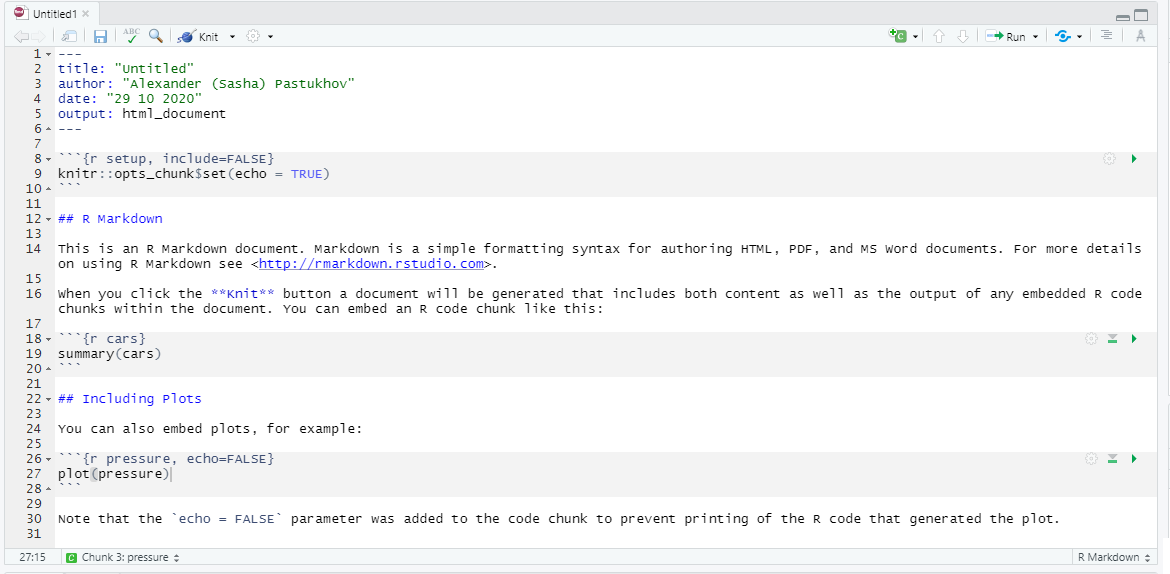
\includegraphics[width=1\linewidth]{images/default-notebook} \end{center}

Let us go through the default notebook that R Studio created for us.

\begin{center}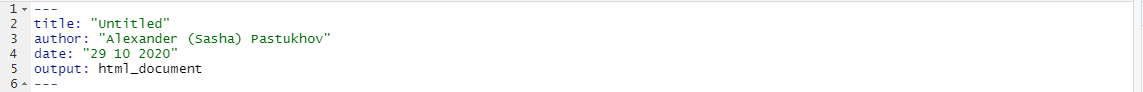
\includegraphics[width=1\linewidth]{images/notebook-header} \end{center}

The top part between two sets of \texttt{-\/-\/-} is a notebook header with various configuration options written in \href{https://yaml.org/}{YAML} (yes, we have two different languages in one file). \texttt{title}, \texttt{author}, and \texttt{date} should be self-explanatory. \texttt{output} defines what kind of output document knitr will generate. You can specify it by hand (e.g., \texttt{word\_document}) or just click on drop down next to \texttt{Knit} button and pick the option you like (we will use the default HTML most of the time). These are sufficient for us but there are numerous other options that you can specify, for example, to enable indexing of headers. You can read about this at \href{https://yihui.org/knitr/}{yihui.org/knitr}.

\begin{center}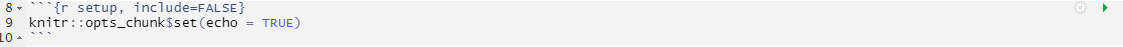
\includegraphics[width=1\linewidth]{images/notebook-setup} \end{center}

The next section is the ``setup code chunk'' that specifies default options for how the code chunks are treated by default (whether they are executed, whether the output, warnings, or messages are shown, etc.). By default code in chunks is run and its output is shown (\texttt{echo\ =\ TRUE}) but you can change this behavior on per-chunk basis by pressing the gear button at the top-right. The setup chunk is also a good place to import your libraries (we will talk about this later) as it is always run before any other chunks (so, even if you forgot to run it to load libraries, R Studio will do this for you).

\begin{center}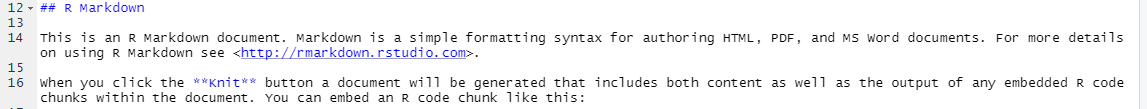
\includegraphics[width=1\linewidth]{images/notebook-text} \end{center}

Next, we have plain text with rmarkdown, which gets translated into formatted text when you click on \emph{Knit} button. You can write like this anywhere outside of code chunks to explain the logic of your analysis. You should write why and how the analysis is performed but leave technical details on programming to the chunk itself, where you can comment the code.

\begin{center}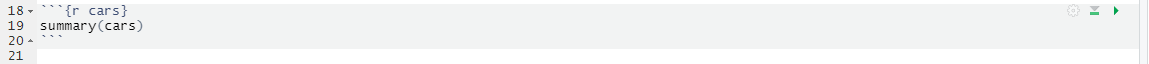
\includegraphics[width=1\linewidth]{images/notebook-chunk} \end{center}

Finally, we have our first ``proper'' chunk of code (the ``setup'' chunk above is a special case). A code chunk is simply the code embedded between
\texttt{\textasciigrave{}\textasciigrave{}\textasciigrave{}\{r\ \textless{}name\ of\ the\ chunk\}} and the seconds set of ticks \texttt{\textasciigrave{}\textasciigrave{}\textasciigrave{}}. Here \texttt{r} specifies that the code inside is written in R language but you can use other languages such as Python (via \href{https://rstudio.github.io/reticulate/}{reticulate} package), \href{https://mc-stan.org/}{Stan}, or SQL. The \texttt{name\ of\ the\ chunk} is optional but I would recommend to specify it, as it reminds you what this code is about and it makes it easier to navigate in large notebooks. In the bottom-left corner, you can see which chunk or section you are currently at and, if you click on it, you can quickly navigate to a different chunk. If chunks are not explicitly named, they will get labels \texttt{Chunk\ 1}, \texttt{Chunk\ 2}, etc. making it hard to distinguish them.

\begin{center}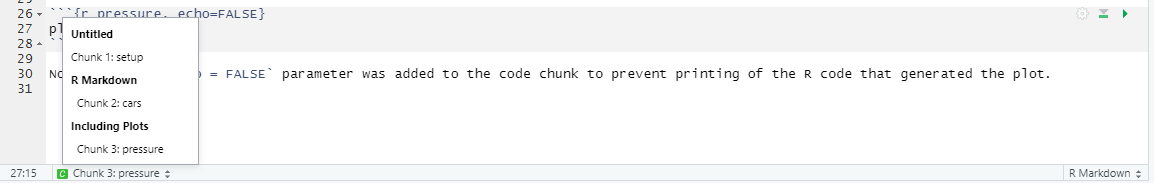
\includegraphics[width=1\linewidth]{images/notebook-navigation} \end{center}

There are additional options that you can specify per chunk (whether to run the code, to show the output, what size the figures should be, etc.). Generally we won't need these options but you can get an idea about them by looking at the \href{https://yihui.org/knitr/options/}{official manual}. You can create a chunk by hand or click on ``Create chunk'' drop-down list (in this case, it will create the chunk at the position of the cursor)

\begin{center}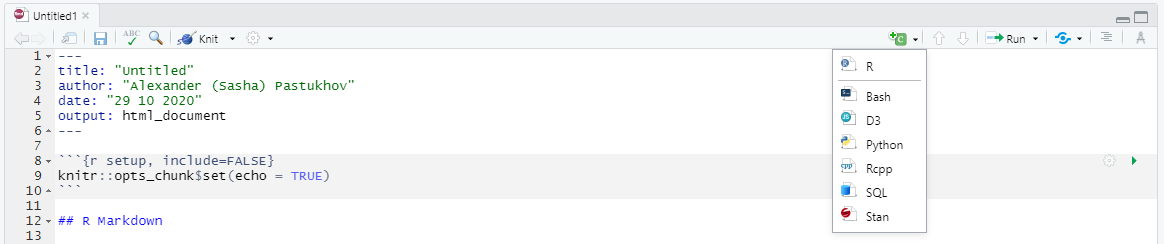
\includegraphics[width=1\linewidth]{images/notebook-insert-chunk} \end{center}

Finally, you run \textbf{all} the code in the chunk by clicking on \emph{Run current chunk button} at the top-right corner of the chunk or by pressing \textbf{Ctrl+Shift+Enter} when the you are inside the chunk. However, you can also run just a \emph{single line} or only \emph{selected lines} by pressing \textbf{Ctrl+Enter}. The cool thing about RMarkdown in RStudio is that you will see the output of that chunk right below it. This means that you can write you code chunk-by-chunk, ensure that each works as intended and only when knit the entire document. Run the chunks in your notebook to see what I mean.

\begin{center}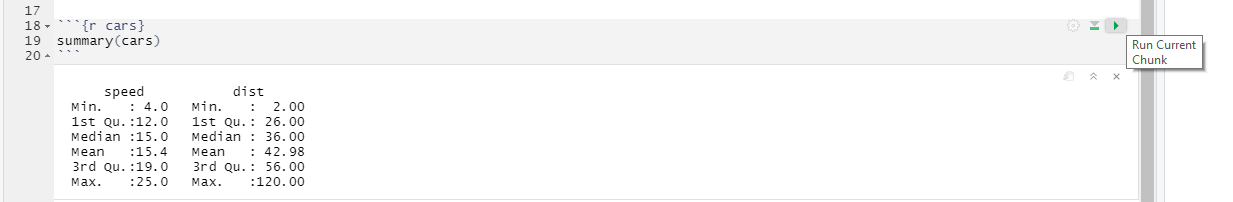
\includegraphics[width=1\linewidth]{images/notebook-run-chunk} \end{center}

\hypertarget{exercise}{%
\section{Exercise}\label{exercise}}

For the today's exercise, I want you to familiarize yourself with markdown. Go to \href{https://www.markdownguide.org/}{markdownguide.org} and look at basic and extended syntax (their cheat sheet is also very good). Write any text you want that uses all the formatting and submit the file to MS Teams.

\hypertarget{vectors}{%
\chapter{Vectors! Vectors everywhere!}\label{vectors}}

Before reading the chapter, please download the \href{notebooks/Seminar\%2002\%20-\%20Vectors.Rmd}{exercise notebook} (\textbf{Alt+Click} to download it or right-click as \emph{Save link as\ldots{}}), put it into your seminar \protect\hyperlink{projects}{project folder}, and open the project. You need both the text and the notebook with exercises to be open, as you will be switching between them.

Before we can start using R for analysis, you need to learn about vectors. This is a key concept in R, so your understanding of it will determine how easy it will be for you to use R in general. Do all of the exercises and do not hesitate to ask me whenever something is unclear. Remember, you need to master vectors before you can master R!

\hypertarget{variables}{%
\section{Variables as boxes}\label{variables}}

In programming, a concept of a variable is often described as a box you can put something in. A box has a name tag on it, which is the \emph{name} of the variable. Whatever you put in is the \emph{value} that you store.

\begin{center}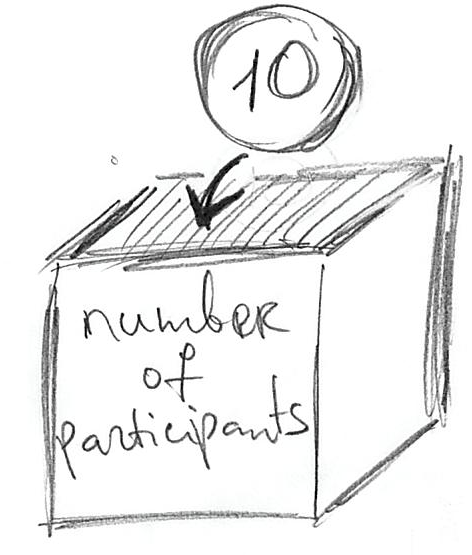
\includegraphics[width=0.3\linewidth]{images/variable-as-box} \end{center}

This ``putting in'' concepts is reflected in R syntax

\begin{Shaded}
\begin{Highlighting}[]
\NormalTok{number\_of\_participants }\OtherTok{\textless{}{-}} \DecValTok{10}
\end{Highlighting}
\end{Shaded}

Here, \texttt{number\_of\_participants} is the name of the variable (name tag for the box that we will be using), \texttt{10} is the value you store, and \texttt{\textless{}-} means \emph{``put \texttt{10} into variable \texttt{number\_of\_participants}''}. If you know other programming languages, you probably expected the usual assignment operator \texttt{=}. Confusingly, you can use it in R as well, but there are some subtle, yet important, \href{https://stat.ethz.ch/R-manual/R-devel/library/base/html/assignOps.html}{differences} in how they operate behind the scenes. We will meet \texttt{=} again when we will be talking about functions and, in particular, Tidyverse way of doing things but for now \textbf{only use \texttt{\textless{}-} operator}!

\hypertarget{assignment-statement}{%
\section{Assignment statement in detail}\label{assignment-statement}}

One \emph{very important} thing to remember about the assignment statement \texttt{\textless{}variable\textgreater{}\ \textless{}-\ \textless{}value\textgreater{}}: The \emph{right side} is evaluated first until the final value is established and then, and only then, it is stored in a \texttt{\textless{}variable\textgreater{}} specified on the left side. This means that you can use the same variable on \emph{both} sides. Take a look at the example

\begin{Shaded}
\begin{Highlighting}[]
\NormalTok{x }\OtherTok{\textless{}{-}} \DecValTok{2}
\FunctionTok{print}\NormalTok{(x)}
\end{Highlighting}
\end{Shaded}

\begin{verbatim}
## [1] 2
\end{verbatim}

\begin{Shaded}
\begin{Highlighting}[]
\NormalTok{x }\OtherTok{\textless{}{-}}\NormalTok{ x }\SpecialCharTok{+} \DecValTok{5}
\FunctionTok{print}\NormalTok{(x)}
\end{Highlighting}
\end{Shaded}

\begin{verbatim}
## [1] 7
\end{verbatim}

We are storing value \texttt{2} in a variable \texttt{x}. In the next line, the \emph{right side} is evaluated first. This means that the current value of \texttt{x} is substituted in its place on the right side: \texttt{x\ +\ 5} becomes \texttt{2\ +\ 5}. This expression computed and we get \texttt{7}. Now, that the \emph{right side} is fully evaluated, the value can be stored in \texttt{x} replacing (overwriting) the original value it had.

R's use of \texttt{\textless{}-} makes it easier to memorize this \emph{right side is fully evaluated first} rule. However, as noted above, we will meet \texttt{=} operator and this one makes it look like a mathematical equation. However, assignments (storing values in a variable) have nothing in common with mathematical equations (finding values of variables to ensure equality)!

Do exercise 1.

\hypertarget{vectors-scalars}{%
\section{Vectors and singluar values (scalars, which are also vectors)}\label{vectors-scalars}}

The box metaphor you've just learned, doesn't quite work for R. Historically, R was developed as a language for statistical computing, so it was based on concepts of linear algebra instead of being a ``normal'' programming language like Python or C. This means that there is no conceptual divide between single values and containers (arrays, lists, dictionaries, etc.) that hold many single values. Instead, the primary data unit in R is a \emph{vector}, which you may remember from geometry or, hopefully, from linear algebra, as an arrow that goes from 0 to a specific point in space. From computer science point of view, a vector is just a list of numbers (or some other values, as you will learn later). This means that there are no ``single values'' in R, there are only vectors of variable length. Special cases are vectors of length one, which are called \emph{scalars} \footnote{Multiplication of a vector by another vector \emph{transforms} it but for a single element vector the only transformation you can get is ``scaling'', hence, the name.} (but they are still vectors) and zero length vectors that are, sort of, a Platonic idea of a vector without actual values. With respect to the ``box metaphor'', this means that we always have a box with indexed (numbered) slots in it. A simple assignment makes sure that ``the box'' has as many slots as values you want to put in and stores these values one after another starting with slot \#1\footnote{If you have experience with programming languages like Python, C, or Java: indexes in R start with 1, not with 0.}. Therefore, the example above \texttt{number\_of\_participants\ \textless{}-\ 10} creates a \emph{vector} variable with one (1) slot and stores the value in it.

\begin{center}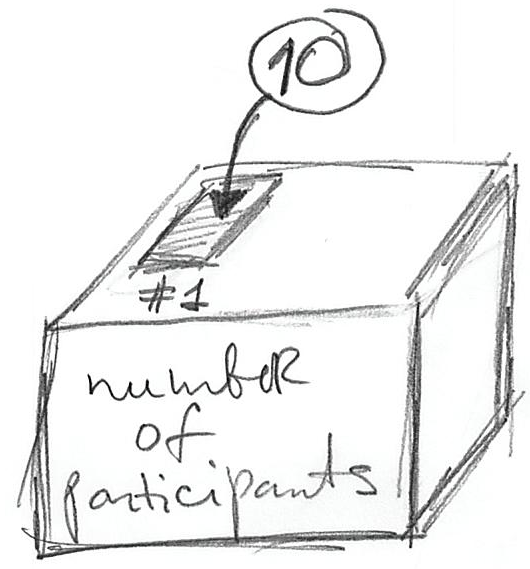
\includegraphics[width=0.3\linewidth]{images/box-with-a-slot} \end{center}

But, as noted above, a single value (vector with length of one) is a special case. More generally you write:

\begin{Shaded}
\begin{Highlighting}[]
\NormalTok{response }\OtherTok{\textless{}{-}} \FunctionTok{c}\NormalTok{(}\DecValTok{1}\NormalTok{, }\DecValTok{7}\NormalTok{, }\DecValTok{3}\NormalTok{)}
\end{Highlighting}
\end{Shaded}

Here, you create a variable (box) named \texttt{response} that has three slots in it because you want to store three values. You put values \texttt{1}, \texttt{7}, \texttt{3} into the slots \#1, \#2, and \#3. The \texttt{c(1,\ 7,\ 3)} notation is how you create a vector in R by \href{https://www.rdocumentation.org/packages/base/versions/3.6.2/topics/c}{\textbf{c}oncatenating} (or \textbf{c}ombining) values\footnote{I find this to be a very poor choice of name but we are stuck with it, so your only option is to get used to it.}. The figure below illustrates the idea:

\begin{center}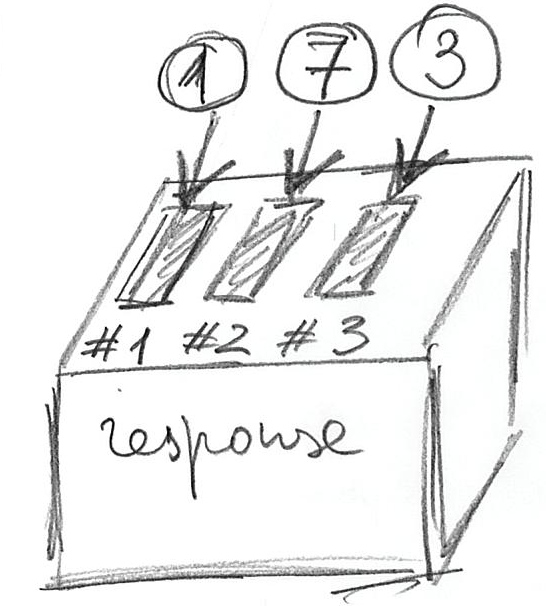
\includegraphics[width=0.3\linewidth]{images/box-3-slots} \end{center}

Building on the box metaphor: If you can store something in a box, you can take it out! In the world of computers it works even better, because rather than taking something out, you just make a copy of that and store this copy somewhere else or to use it to compute things. Minimally, we would like to see what is inside of the box. For this, you can use \href{https://stat.ethz.ch/R-manual/R-devel/library/base/html/print.html}{print} function:

\begin{Shaded}
\begin{Highlighting}[]
\NormalTok{response }\OtherTok{\textless{}{-}} \FunctionTok{c}\NormalTok{(}\DecValTok{1}\NormalTok{, }\DecValTok{7}\NormalTok{, }\DecValTok{3}\NormalTok{)}
\FunctionTok{print}\NormalTok{(response)}
\end{Highlighting}
\end{Shaded}

\begin{verbatim}
## [1] 1 7 3
\end{verbatim}

Or, we can make a copy of values in one variable and store them in another:

\begin{Shaded}
\begin{Highlighting}[]
\NormalTok{x }\OtherTok{\textless{}{-}} \FunctionTok{c}\NormalTok{(}\DecValTok{3}\NormalTok{, }\DecValTok{6}\NormalTok{, }\DecValTok{9}\NormalTok{)}
\NormalTok{y }\OtherTok{\textless{}{-}}\NormalTok{ x }

\FunctionTok{print}\NormalTok{(x)}
\end{Highlighting}
\end{Shaded}

\begin{verbatim}
## [1] 3 6 9
\end{verbatim}

\begin{Shaded}
\begin{Highlighting}[]
\FunctionTok{print}\NormalTok{(y)}
\end{Highlighting}
\end{Shaded}

\begin{verbatim}
## [1] 3 6 9
\end{verbatim}

Here, we create a 3-slot variable \texttt{x} so that we can put in a vector of length 3 created via concatenation \texttt{c(3,\ 6,\ 9)}. Next, we make a copy of these three values and store them in a different variable \texttt{y}. Importantly, the values in variable \texttt{x} stayed as they were. Take a look at the figure below, which graphically illustrate this:

\begin{center}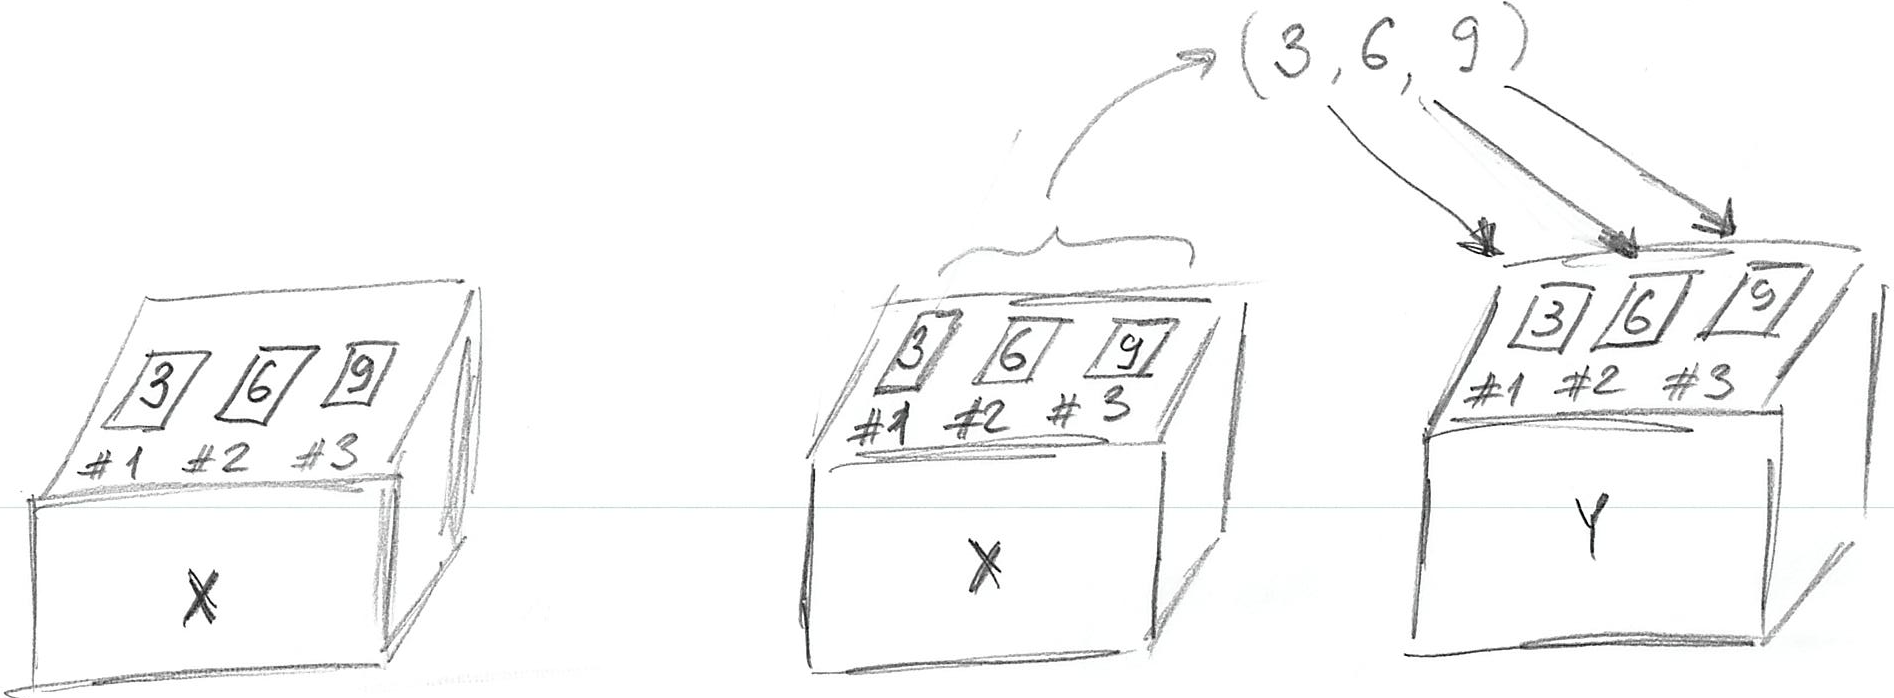
\includegraphics[width=1\linewidth]{images/copy-vector} \end{center}

Do exercise 2.

Remember, everything is a vector! This means that \texttt{c(3,\ 6,\ 9)} does not concatenate numbers, it concatenates three length one vectors (scalars) \texttt{3}, \texttt{6}, \texttt{9}. Thus, concatenation works on longer vectors in exactly the same way:

\begin{Shaded}
\begin{Highlighting}[]
\NormalTok{x }\OtherTok{\textless{}{-}} \FunctionTok{c}\NormalTok{(}\DecValTok{1}\NormalTok{, }\DecValTok{2}\NormalTok{, }\DecValTok{3}\NormalTok{)}
\NormalTok{y }\OtherTok{\textless{}{-}} \FunctionTok{c}\NormalTok{(}\DecValTok{4}\NormalTok{, }\DecValTok{5}\NormalTok{)}
\FunctionTok{print}\NormalTok{(}\FunctionTok{c}\NormalTok{(x, y))}
\end{Highlighting}
\end{Shaded}

\begin{verbatim}
## [1] 1 2 3 4 5
\end{verbatim}

Do exercise 3.

\hypertarget{vector-index}{%
\section{Vector indexes (subsetting)}\label{vector-index}}

A vector is an ordered list of values (box with some slots) and, sometimes, you need only one of the values. Each value (slot in the box) has its own index from 1 till N, where N is the \href{https://stat.ethz.ch/R-manual/R-devel/library/base/html/length.html}{length} of the vector. To access that slot you use square brackets \texttt{some\_vector{[}index{]}}. You can both get and set the value for the individual slots the same way you do it for the whole vector.

\begin{Shaded}
\begin{Highlighting}[]
\NormalTok{x }\OtherTok{\textless{}{-}} \FunctionTok{c}\NormalTok{(}\DecValTok{1}\NormalTok{, }\DecValTok{2}\NormalTok{, }\DecValTok{3}\NormalTok{)}
\CommentTok{\# set SECOND element to 4}
\NormalTok{x[}\DecValTok{2}\NormalTok{] }\OtherTok{\textless{}{-}} \DecValTok{4}

\CommentTok{\# print the entire vector}
\FunctionTok{print}\NormalTok{(x)}
\end{Highlighting}
\end{Shaded}

\begin{verbatim}
## [1] 1 4 3
\end{verbatim}

\begin{Shaded}
\begin{Highlighting}[]
\CommentTok{\# print only the third element}
\FunctionTok{print}\NormalTok{(x[}\DecValTok{3}\NormalTok{])}
\end{Highlighting}
\end{Shaded}

\begin{verbatim}
## [1] 3
\end{verbatim}

Do exercise 4.

Unfortunately, vector indexing in R behaves in a way that may\footnote{Who am I kidding? Will!} catch you by surprise. Or, even worse, you will not even notice that your indexing does not work and screwes up your analysis. If your vector contains five values, you would expect that an index of \texttt{0} (negative indexes are special and will be discussed below) or above \texttt{5} generates an error. Not in R! Index of \texttt{0} is a special case and produces an \emph{empty vector} (vector of zero length).

\begin{Shaded}
\begin{Highlighting}[]
\NormalTok{x }\OtherTok{\textless{}{-}} \FunctionTok{c}\NormalTok{(}\DecValTok{1}\NormalTok{, }\DecValTok{2}\NormalTok{, }\DecValTok{3}\NormalTok{)}
\NormalTok{x[}\DecValTok{0}\NormalTok{]}
\end{Highlighting}
\end{Shaded}

\begin{verbatim}
## numeric(0)
\end{verbatim}

If you try to get vector element using index that is larger than vector length (so \texttt{6} and above for a 5 element vector), R will return \texttt{NA} (\href{https://stat.ethz.ch/R-manual/R-devel/library/base/html/NA.html}{``Not Available'' / Missing Value}).

\begin{Shaded}
\begin{Highlighting}[]
\NormalTok{x }\OtherTok{\textless{}{-}} \FunctionTok{c}\NormalTok{(}\DecValTok{1}\NormalTok{, }\DecValTok{2}\NormalTok{, }\DecValTok{3}\NormalTok{)}
\NormalTok{x[}\DecValTok{5}\NormalTok{]}
\end{Highlighting}
\end{Shaded}

\begin{verbatim}
## [1] NA
\end{verbatim}

In both cases, it won't generate an error or even warn you!

When \emph{setting} a value by index, using \texttt{0} will produce no effect, because you are trying to put a value into a vector with no ``slots''. Oddly enough, this will also generate neither an error nor a warning, so beware!

\begin{Shaded}
\begin{Highlighting}[]
\NormalTok{x }\OtherTok{\textless{}{-}} \FunctionTok{c}\NormalTok{(}\DecValTok{1}\NormalTok{, }\DecValTok{2}\NormalTok{, }\DecValTok{3}\NormalTok{)}
\NormalTok{x[}\DecValTok{0}\NormalTok{] }\OtherTok{\textless{}{-}} \DecValTok{5}
\FunctionTok{print}\NormalTok{(x)}
\end{Highlighting}
\end{Shaded}

\begin{verbatim}
## [1] 1 2 3
\end{verbatim}

If you set an element with index \textbf{larger} than vector length, the vector will be automatically expanded to that length and all the elements between the old values and the new one will be \texttt{NA} (\href{https://stat.ethz.ch/R-manual/R-devel/library/base/html/NA.html}{``Not Available'' / Missing Value}).

\begin{Shaded}
\begin{Highlighting}[]
\NormalTok{x }\OtherTok{\textless{}{-}} \FunctionTok{c}\NormalTok{(}\DecValTok{1}\NormalTok{, }\DecValTok{2}\NormalTok{, }\DecValTok{3}\NormalTok{)}
\NormalTok{x[}\DecValTok{10}\NormalTok{] }\OtherTok{\textless{}{-}} \DecValTok{5}
\FunctionTok{print}\NormalTok{(x)}
\end{Highlighting}
\end{Shaded}

\begin{verbatim}
##  [1]  1  2  3 NA NA NA NA NA NA  5
\end{verbatim}

This may sound too technical but I want you to learn about this because R conventions are so different from other programming languages and, also, from what you would intuitively expect. If you are not aware of these highly peculiar rules, you may never realize that your code is not working properly because, remember, you will never see an error or even a warning! It should also make you more cautious and careful when programming in R. It is a very powerful language that allows you to be very flexible and expressive. Unfortunately, that flexibility means that base R won't stop you from shooting yourself in a foot. Even worse, sometimes you won't even notice that your foot is shot and bleeding because R won't generate either errors or warnings, as in examples above. Good news is that things are far more restricted and consistent in Tidyverse.

Do exercise 5.

You can also use \emph{negative} indexes. In that case, you \emph{exclude} the value with that index and return or modify the rest\footnote{People who use Python, please be aware that negatives indexes in R and in Python behave completely differently!}.

\begin{Shaded}
\begin{Highlighting}[]
\NormalTok{x }\OtherTok{\textless{}{-}} \FunctionTok{c}\NormalTok{(}\DecValTok{1}\NormalTok{, }\DecValTok{2}\NormalTok{, }\DecValTok{3}\NormalTok{, }\DecValTok{4}\NormalTok{, }\DecValTok{5}\NormalTok{)}
\CommentTok{\# this will return all elements but \#3}
\NormalTok{x[}\SpecialCharTok{{-}}\DecValTok{3}\NormalTok{] }
\end{Highlighting}
\end{Shaded}

\begin{verbatim}
## [1] 1 2 4 5
\end{verbatim}

\begin{Shaded}
\begin{Highlighting}[]
\NormalTok{x }\OtherTok{\textless{}{-}} \FunctionTok{c}\NormalTok{(}\DecValTok{1}\NormalTok{, }\DecValTok{2}\NormalTok{, }\DecValTok{3}\NormalTok{, }\DecValTok{4}\NormalTok{, }\DecValTok{5}\NormalTok{)}
\CommentTok{\# this will assign new value (by repeating length one vector) to all elements but \#2}
\NormalTok{x[}\SpecialCharTok{{-}}\DecValTok{2}\NormalTok{] }\OtherTok{\textless{}{-}} \DecValTok{10}
\NormalTok{x}
\end{Highlighting}
\end{Shaded}

\begin{verbatim}
## [1] 10  2 10 10 10
\end{verbatim}

Given that negative indexing returns everything \textbf{but} the indexed value, what do you think will happen here?

\begin{Shaded}
\begin{Highlighting}[]
\NormalTok{x }\OtherTok{\textless{}{-}} \FunctionTok{c}\NormalTok{(}\DecValTok{10}\NormalTok{, }\DecValTok{20}\NormalTok{, }\DecValTok{30}\NormalTok{, }\DecValTok{40}\NormalTok{, }\DecValTok{50}\NormalTok{)}
\NormalTok{x[}\SpecialCharTok{{-}}\DecValTok{10}\NormalTok{]}
\end{Highlighting}
\end{Shaded}

Do exercise 6.

Finally, somewhat counterintuitively, the entire vector is returned if you do not specify an index in the square brackets. Here, lack of index means ``everything''.

\begin{Shaded}
\begin{Highlighting}[]
\NormalTok{x }\OtherTok{\textless{}{-}} \FunctionTok{c}\NormalTok{(}\DecValTok{10}\NormalTok{, }\DecValTok{20}\NormalTok{, }\DecValTok{30}\NormalTok{, }\DecValTok{40}\NormalTok{, }\DecValTok{50}\NormalTok{)}
\NormalTok{x[]}
\end{Highlighting}
\end{Shaded}

\begin{verbatim}
## [1] 10 20 30 40 50
\end{verbatim}

\hypertarget{names}{%
\section{Names as an Index}\label{names}}

As you've just learned, every slot in vector has its numeric (integer) index. However, this number only indicates an index (position) of a slot but tells you nothing on how it is conceptually different from a slot with a different index. For example, if we are storing width and height in a vector, remembering their order may be tricky: was it \texttt{box\_size\ \textless{}-\ c(\textless{}width\textgreater{},\ \textless{}depth\textgreater{},\ \textless{}height\textgreater{})} or \texttt{box\_size\ \textless{}-\ c(\textless{}height\textgreater{},\ \textless{}width\textgreater{},\ \textless{}depth\textgreater{})}? Similarly, looking at \texttt{box\_size{[}1{]}} tells that you are definitely using the \emph{first} dimension but is it \texttt{height} or \texttt{width} (or \texttt{depth})?

In R, you can use \href{https://stat.ethz.ch/R-manual/R-devel/library/base/html/names.html}{names} to supplement numeric indexes. It allows you to add meaning to a particular vector index, something that becomes extremely important when we use it for tables. There are two ways to assign names to indexes, either when you are creating the index via \href{https://stat.ethz.ch/R-manual/R-devel/library/base/html/c.html}{c()} function or, afterwards, via \href{https://stat.ethz.ch/R-manual/R-devel/library/base/html/names.html}{names()} function.

To create named vector via \href{https://stat.ethz.ch/R-manual/R-devel/library/base/html/c.html}{c()} you specify a name before each value as \texttt{c(\textless{}name1\textgreater{}\ =\ \textless{}value1\textgreater{},\ \textless{}name2\textgreater{}\ =\ \textless{}value2\textgreater{},\ ...)}:

\begin{Shaded}
\begin{Highlighting}[]
\NormalTok{box\_size }\OtherTok{\textless{}{-}} \FunctionTok{c}\NormalTok{(}\StringTok{"width"}\OtherTok{=}\DecValTok{2}\NormalTok{, }\StringTok{"height"}\OtherTok{=}\DecValTok{4}\NormalTok{, }\StringTok{"depth"}\OtherTok{=}\DecValTok{1}\NormalTok{) }
\FunctionTok{print}\NormalTok{(box\_size)}
\end{Highlighting}
\end{Shaded}

\begin{verbatim}
##  width height  depth 
##      2      4      1
\end{verbatim}

Note the names appearing above each value. You can now use either numeric index or name to access the value.

\begin{Shaded}
\begin{Highlighting}[]
\NormalTok{box\_size }\OtherTok{\textless{}{-}} \FunctionTok{c}\NormalTok{(}\StringTok{"width"}\OtherTok{=}\DecValTok{2}\NormalTok{, }\StringTok{"height"}\OtherTok{=}\DecValTok{4}\NormalTok{, }\StringTok{"depth"}\OtherTok{=}\DecValTok{1}\NormalTok{) }
\FunctionTok{print}\NormalTok{(box\_size[}\DecValTok{1}\NormalTok{])}
\end{Highlighting}
\end{Shaded}

\begin{verbatim}
## width 
##     2
\end{verbatim}

\begin{Shaded}
\begin{Highlighting}[]
\FunctionTok{print}\NormalTok{(box\_size[}\StringTok{"depth"}\NormalTok{])}
\end{Highlighting}
\end{Shaded}

\begin{verbatim}
## depth 
##     1
\end{verbatim}

Alternatively, you can use \href{https://stat.ethz.ch/R-manual/R-devel/library/base/html/names.html}{names()} function to both get and set the names. The latter works via a \emph{very counterintuitive} syntax \texttt{names(\textless{}vector\textgreater{})\ \textless{}-\ \textless{}vector-with-names\textgreater{}}

\begin{Shaded}
\begin{Highlighting}[]
\CommentTok{\# without names}
\NormalTok{box\_size }\OtherTok{\textless{}{-}} \FunctionTok{c}\NormalTok{(}\DecValTok{2}\NormalTok{, }\DecValTok{4}\NormalTok{, }\DecValTok{1}\NormalTok{) }
\FunctionTok{print}\NormalTok{(box\_size)}
\end{Highlighting}
\end{Shaded}

\begin{verbatim}
## [1] 2 4 1
\end{verbatim}

\begin{Shaded}
\begin{Highlighting}[]
\CommentTok{\# with names}
\FunctionTok{names}\NormalTok{(box\_size) }\OtherTok{\textless{}{-}} \FunctionTok{c}\NormalTok{(}\StringTok{"width"}\NormalTok{, }\StringTok{"height"}\NormalTok{, }\StringTok{"depth"}\NormalTok{)}
\FunctionTok{print}\NormalTok{(box\_size)}
\end{Highlighting}
\end{Shaded}

\begin{verbatim}
##  width height  depth 
##      2      4      1
\end{verbatim}

\begin{Shaded}
\begin{Highlighting}[]
\CommentTok{\# getting all the names}
\FunctionTok{print}\NormalTok{(}\FunctionTok{names}\NormalTok{(box\_size))}
\end{Highlighting}
\end{Shaded}

\begin{verbatim}
## [1] "width"  "height" "depth"
\end{verbatim}

Because everything is a vector, \texttt{names(\textless{}vector\textgreater{})} is also a vector, meaning that you can get or set just one element of it.

\begin{Shaded}
\begin{Highlighting}[]
\NormalTok{box\_size }\OtherTok{\textless{}{-}} \FunctionTok{c}\NormalTok{(}\StringTok{"width"}\OtherTok{=}\DecValTok{2}\NormalTok{, }\StringTok{"height"}\OtherTok{=}\DecValTok{4}\NormalTok{, }\StringTok{"depth"}\OtherTok{=}\DecValTok{1}\NormalTok{) }

\CommentTok{\# modify SECOND name}
\FunctionTok{names}\NormalTok{(box\_size)[}\DecValTok{2}\NormalTok{] }\OtherTok{\textless{}{-}} \StringTok{"HEIGHT"}
\FunctionTok{print}\NormalTok{(box\_size)}
\end{Highlighting}
\end{Shaded}

\begin{verbatim}
##  width HEIGHT  depth 
##      2      4      1
\end{verbatim}

Finally, if you use a name that is not in the index, this is like using numeric index larger than the vector length. Just as for out-of-range numeric index, there will be neither error not warning and you will get an \texttt{NA} back.

\begin{Shaded}
\begin{Highlighting}[]
\NormalTok{box\_size }\OtherTok{\textless{}{-}} \FunctionTok{c}\NormalTok{(}\StringTok{"width"}\OtherTok{=}\DecValTok{2}\NormalTok{, }\StringTok{"height"}\OtherTok{=}\DecValTok{4}\NormalTok{, }\StringTok{"depth"}\OtherTok{=}\DecValTok{1}\NormalTok{) }
\FunctionTok{print}\NormalTok{(box\_size[}\StringTok{"radius"}\NormalTok{])}
\end{Highlighting}
\end{Shaded}

\begin{verbatim}
## <NA> 
##   NA
\end{verbatim}

Do exercise 7.

\hypertarget{vector-index-slicing}{%
\section{Slicing}\label{vector-index-slicing}}

So far we were reading or modifying either the whole vector or just one of its elements. However, the index you pass in square brackets (you've guess it!) is also a vector! Which means that you can construct a vector of indexes the same way you construct a vector of any values (the only restriction is that index values must integers and that you cannot mix negative and positive indexes).

\begin{Shaded}
\begin{Highlighting}[]
\NormalTok{x }\OtherTok{\textless{}{-}} \FunctionTok{c}\NormalTok{(}\DecValTok{10}\NormalTok{, }\DecValTok{20}\NormalTok{, }\DecValTok{30}\NormalTok{, }\DecValTok{40}\NormalTok{, }\DecValTok{50}\NormalTok{)}
\NormalTok{x[}\FunctionTok{c}\NormalTok{(}\DecValTok{2}\NormalTok{, }\DecValTok{3}\NormalTok{, }\DecValTok{5}\NormalTok{)]}
\end{Highlighting}
\end{Shaded}

\begin{verbatim}
## [1] 20 30 50
\end{verbatim}

When constructing a vector index, you can put index values in the order you require (normal ascending order, starting from the end of it, random order, etc.) or use the same index more than once.

\begin{Shaded}
\begin{Highlighting}[]
\NormalTok{x }\OtherTok{\textless{}{-}} \FunctionTok{c}\NormalTok{(}\DecValTok{10}\NormalTok{, }\DecValTok{20}\NormalTok{, }\DecValTok{30}\NormalTok{, }\DecValTok{40}\NormalTok{, }\DecValTok{50}\NormalTok{)}
\NormalTok{x[}\FunctionTok{c}\NormalTok{(}\DecValTok{3}\NormalTok{, }\DecValTok{5}\NormalTok{, }\DecValTok{1}\NormalTok{, }\DecValTok{1}\NormalTok{, }\DecValTok{4}\NormalTok{)]}
\end{Highlighting}
\end{Shaded}

\begin{verbatim}
## [1] 30 50 10 10 40
\end{verbatim}

You can also use several negative indexes to exclude multiple values and return the rest. Here, neither order nor duplicate indexes matter. Regardless of which value you exclude first or how many times you exclude it, you still get \emph{the rest} of the vector in its default order.

\begin{Shaded}
\begin{Highlighting}[]
\NormalTok{x }\OtherTok{\textless{}{-}} \FunctionTok{c}\NormalTok{(}\DecValTok{10}\NormalTok{, }\DecValTok{20}\NormalTok{, }\DecValTok{30}\NormalTok{, }\DecValTok{40}\NormalTok{, }\DecValTok{50}\NormalTok{)}
\NormalTok{x[}\FunctionTok{c}\NormalTok{(}\SpecialCharTok{{-}}\DecValTok{4}\NormalTok{, }\SpecialCharTok{{-}}\DecValTok{2}\NormalTok{, }\SpecialCharTok{{-}}\DecValTok{2}\NormalTok{)]}
\end{Highlighting}
\end{Shaded}

\begin{verbatim}
## [1] 10 30 50
\end{verbatim}

Note that you cannot mix positive and negative indexes as R will generate an error (at last!).

\begin{Shaded}
\begin{Highlighting}[]
\NormalTok{x }\OtherTok{\textless{}{-}} \FunctionTok{c}\NormalTok{(}\DecValTok{10}\NormalTok{, }\DecValTok{20}\NormalTok{, }\DecValTok{30}\NormalTok{, }\DecValTok{40}\NormalTok{, }\DecValTok{50}\NormalTok{)}

\CommentTok{\# THIS WILL GENERATE AN ERROR: }
\CommentTok{\# "Error in x[c({-}4, 2, {-}2)] : only 0\textquotesingle{}s may be mixed with negative subscripts"}
\NormalTok{x[}\FunctionTok{c}\NormalTok{(}\SpecialCharTok{{-}}\DecValTok{4}\NormalTok{, }\DecValTok{2}\NormalTok{, }\SpecialCharTok{{-}}\DecValTok{2}\NormalTok{)]}
\end{Highlighting}
\end{Shaded}

Finally, including zero index makes no difference but generates neither an error nor a warning.

\begin{Shaded}
\begin{Highlighting}[]
\NormalTok{x }\OtherTok{\textless{}{-}} \FunctionTok{c}\NormalTok{(}\DecValTok{10}\NormalTok{, }\DecValTok{20}\NormalTok{, }\DecValTok{30}\NormalTok{, }\DecValTok{40}\NormalTok{, }\DecValTok{50}\NormalTok{)}
\NormalTok{x[}\FunctionTok{c}\NormalTok{(}\DecValTok{1}\NormalTok{, }\DecValTok{0}\NormalTok{, }\DecValTok{5}\NormalTok{, }\DecValTok{0}\NormalTok{, }\DecValTok{0}\NormalTok{, }\DecValTok{2}\NormalTok{, }\DecValTok{2}\NormalTok{)]}
\end{Highlighting}
\end{Shaded}

\begin{verbatim}
## [1] 10 50 20 20
\end{verbatim}

You can also use names instead of numeric indexes.

\begin{Shaded}
\begin{Highlighting}[]
\NormalTok{box\_size }\OtherTok{\textless{}{-}} \FunctionTok{c}\NormalTok{(}\StringTok{"width"}\OtherTok{=}\DecValTok{2}\NormalTok{, }\StringTok{"height"}\OtherTok{=}\DecValTok{4}\NormalTok{, }\StringTok{"depth"}\OtherTok{=}\DecValTok{1}\NormalTok{) }
\FunctionTok{print}\NormalTok{(box\_size[}\FunctionTok{c}\NormalTok{(}\StringTok{"height"}\NormalTok{, }\StringTok{"width"}\NormalTok{)])}
\end{Highlighting}
\end{Shaded}

\begin{verbatim}
## height  width 
##      4      2
\end{verbatim}

However, you cannot mix numeric indexes and names. The reason is that a vector can hold only values of one type (more on that next time), so all numeric values will be converted to text (\texttt{1} will become \texttt{"1"}) and treated as names rather than indexes.

\hypertarget{colon-sequence}{%
\section{Colon Operator and Sequence Generation}\label{colon-sequence}}

To simplify vector indexing, R provides you with a shortcut to create a range of values. An expression \texttt{A:B} (a.k.a.\href{https://stat.ethz.ch/R-manual/R-devel/library/base/html/Colon.html}{Colon Operator}) builds a sequence of integers starting with \texttt{A} and ending with \textbf{and including(!)} \texttt{B}\footnote{The latter is not so obvious, if you come from Python}.

\begin{Shaded}
\begin{Highlighting}[]
\DecValTok{3}\SpecialCharTok{:}\DecValTok{7}
\end{Highlighting}
\end{Shaded}

\begin{verbatim}
## [1] 3 4 5 6 7
\end{verbatim}

Thus, you can use it to easily create an index and, because everything is a vector!, combine it with other values.

\begin{Shaded}
\begin{Highlighting}[]
\NormalTok{x }\OtherTok{\textless{}{-}} \FunctionTok{c}\NormalTok{(}\DecValTok{10}\NormalTok{, }\DecValTok{20}\NormalTok{, }\DecValTok{30}\NormalTok{, }\DecValTok{40}\NormalTok{, }\DecValTok{50}\NormalTok{)}
\NormalTok{x[}\FunctionTok{c}\NormalTok{(}\DecValTok{1}\NormalTok{, }\DecValTok{3}\SpecialCharTok{:}\DecValTok{5}\NormalTok{)]}
\end{Highlighting}
\end{Shaded}

\begin{verbatim}
## [1] 10 30 40 50
\end{verbatim}

The sequence above is increasing but you can also use the colon operator to construct a decreasing one.

\begin{Shaded}
\begin{Highlighting}[]
\NormalTok{x }\OtherTok{\textless{}{-}} \FunctionTok{c}\NormalTok{(}\DecValTok{10}\NormalTok{, }\DecValTok{20}\NormalTok{, }\DecValTok{30}\NormalTok{, }\DecValTok{40}\NormalTok{, }\DecValTok{50}\NormalTok{)}
\NormalTok{x[}\FunctionTok{c}\NormalTok{(}\DecValTok{5}\SpecialCharTok{:}\DecValTok{2}\NormalTok{)]}
\end{Highlighting}
\end{Shaded}

\begin{verbatim}
## [1] 50 40 30 20
\end{verbatim}

The colon operator is limited to sequences with steps of \texttt{1} (if end value is larger than the start value) or \texttt{-1} (if end value is smaller than the start value). For more flexibility you can use \href{https://stat.ethz.ch/R-manual/R-devel/library/base/html/seq.html}{Sequence Generation} function: \texttt{seq(from,\ to,\ by,\ length.out)}. The \texttt{from} and \texttt{to} are starting and ending values (just like in the colon operator) and you can specify either a step via \texttt{by} parameter (as, in ``from A to B by C'') or via \texttt{length.out} parameter (how many values you want to generate, effectively \texttt{by\ =\ ((to\ -\ from)/(length.out\ -\ 1)}).
Using \texttt{by} version:

\begin{Shaded}
\begin{Highlighting}[]
\FunctionTok{seq}\NormalTok{(}\DecValTok{1}\NormalTok{, }\DecValTok{5}\NormalTok{, }\AttributeTok{by=}\DecValTok{2}\NormalTok{)}
\end{Highlighting}
\end{Shaded}

\begin{verbatim}
## [1] 1 3 5
\end{verbatim}

Same sequence but using \texttt{length.out} version:

\begin{Shaded}
\begin{Highlighting}[]
\FunctionTok{seq}\NormalTok{(}\DecValTok{1}\NormalTok{, }\DecValTok{5}\NormalTok{, }\AttributeTok{length.out=}\DecValTok{3}\NormalTok{)}
\end{Highlighting}
\end{Shaded}

\begin{verbatim}
## [1] 1 3 5
\end{verbatim}

You have probably spotted the \texttt{=} symbol. Here, it is not an assignment but is used to specify values of parameters when you call a function. Thus, we are still sticking with \texttt{\textless{}-} \textbf{outside} of the function \emph{calls} but are using \texttt{=} \textbf{inside} the function calls.

Do exercise 8.

\hypertarget{working-with-two-vectors-of-equal-length}{%
\section{\texorpdfstring{Working with two vectors of \emph{equal} length}{Working with two vectors of equal length}}\label{working-with-two-vectors-of-equal-length}}

You can also use mathematical operations on several vectors. Here, vectors are matched element-wise. Thus, if you add two vectors of \emph{equal} length, the \emph{first} element of the first vector is added to the \emph{first} element of the second vector, \emph{second} element to \emph{second}, etc.

\begin{Shaded}
\begin{Highlighting}[]
\NormalTok{x }\OtherTok{\textless{}{-}} \FunctionTok{c}\NormalTok{(}\DecValTok{1}\NormalTok{, }\DecValTok{4}\NormalTok{, }\DecValTok{5}\NormalTok{)}
\NormalTok{y }\OtherTok{\textless{}{-}} \FunctionTok{c}\NormalTok{(}\DecValTok{2}\NormalTok{, }\DecValTok{7}\NormalTok{, }\SpecialCharTok{{-}}\DecValTok{3}\NormalTok{)}
\NormalTok{z }\OtherTok{\textless{}{-}}\NormalTok{ x }\SpecialCharTok{+}\NormalTok{ y}
\FunctionTok{print}\NormalTok{(z)}
\end{Highlighting}
\end{Shaded}

\begin{verbatim}
## [1]  3 11  2
\end{verbatim}

Do exercise 9.

\hypertarget{different-length-vectors}{%
\section{\texorpdfstring{Working with two vectors of \emph{different} length}{Working with two vectors of different length}}\label{different-length-vectors}}

What if vectors are of \emph{different} length? If the length of the longer vector is a \emph{multiple} of the shorter vector length, the shorter vector is repeated N-times (where \(N = length(longer~vector) / length(shorter~vector)\)) and this length-matched vector is then used for the mathematical operation. Take a look at the results of the following computation

\begin{Shaded}
\begin{Highlighting}[]
\NormalTok{x }\OtherTok{\textless{}{-}} \DecValTok{1}\SpecialCharTok{:}\DecValTok{6}
\NormalTok{y }\OtherTok{\textless{}{-}} \FunctionTok{c}\NormalTok{(}\DecValTok{2}\NormalTok{, }\DecValTok{3}\NormalTok{)}
\FunctionTok{print}\NormalTok{(x }\SpecialCharTok{+}\NormalTok{ y)}
\end{Highlighting}
\end{Shaded}

\begin{verbatim}
## [1] 3 5 5 7 7 9
\end{verbatim}

Here, the values of \texttt{y} were repeated three times to match the length of \texttt{x}, so the actual computation was \texttt{c(1,\ 2,\ 3,\ 4,\ 5,\ 6)\ +\ c(2,\ 3,\ 2,\ 3,\ 2,\ 3)}. A vector of length 1 (scalar) is a special case because any integer is a multiple of 1, so that single value is repeated \texttt{length(longer\_vector)} times before the operation is performed.

\begin{Shaded}
\begin{Highlighting}[]
\NormalTok{x }\OtherTok{\textless{}{-}} \DecValTok{1}\SpecialCharTok{:}\DecValTok{6}
\NormalTok{y }\OtherTok{\textless{}{-}} \DecValTok{2}
\FunctionTok{print}\NormalTok{(x }\SpecialCharTok{+}\NormalTok{ y)}
\end{Highlighting}
\end{Shaded}

\begin{verbatim}
## [1] 3 4 5 6 7 8
\end{verbatim}

Again, the actual computation is \texttt{c(1,\ 2,\ 3,\ 4,\ 5,\ 6)\ +\ c(2,\ 2,\ 2,\ 2,\ 2,\ 2)}.

If the length of the longer vector \textbf{is not} a multiple of the shorter vector length, R will repeat the shorter vector N times, so that \(N = ceiling(length(longer~vector) / length(shorter~vector))\) (where \href{https://stat.ethz.ch/R-manual/R-devel/library/base/html/Round.html}{ceiling()} rounds a number up) and truncates (throws away) extra elements it does not need. Although R will do it, it will also issue a warning (yay!) about mismatching objects' (vectors') lengths.

\begin{Shaded}
\begin{Highlighting}[]
\NormalTok{x }\OtherTok{\textless{}{-}} \FunctionTok{c}\NormalTok{(}\DecValTok{2}\NormalTok{, }\DecValTok{3}\NormalTok{)}
\NormalTok{y }\OtherTok{\textless{}{-}} \FunctionTok{c}\NormalTok{(}\DecValTok{1}\NormalTok{, }\DecValTok{1}\NormalTok{, }\DecValTok{1}\NormalTok{, }\DecValTok{1}\NormalTok{, }\DecValTok{1}\NormalTok{)}
\FunctionTok{print}\NormalTok{(x }\SpecialCharTok{+}\NormalTok{ y)}
\end{Highlighting}
\end{Shaded}

\begin{verbatim}
## Warning in x + y: longer object length is not a multiple of shorter object
## length
\end{verbatim}

\begin{verbatim}
## [1] 3 4 3 4 3
\end{verbatim}

Finally, combining any vector with null length vector produces a null length vector\footnote{No idea!}.

\begin{Shaded}
\begin{Highlighting}[]
\NormalTok{x }\OtherTok{\textless{}{-}} \FunctionTok{c}\NormalTok{(}\DecValTok{2}\NormalTok{, }\DecValTok{3}\NormalTok{)}
\NormalTok{y }\OtherTok{\textless{}{-}} \FunctionTok{c}\NormalTok{(}\DecValTok{1}\NormalTok{, }\DecValTok{1}\NormalTok{, }\DecValTok{1}\NormalTok{, }\DecValTok{1}\NormalTok{, }\DecValTok{1}\NormalTok{)}
\FunctionTok{print}\NormalTok{(x }\SpecialCharTok{+}\NormalTok{ y[}\DecValTok{0}\NormalTok{])}
\end{Highlighting}
\end{Shaded}

\begin{verbatim}
## numeric(0)
\end{verbatim}

One thing to keep in mind: R does this length-matching-via-vector-repetition automatically and shows a warning only if two lengths are not multiples of each other. This means that vectors will be matched by length even if that was not your plan. Imagine that your vector, which contains experimental condition (e.g.~contrast of the stimulus), is about all ten blocks that participants performed but your vector with responses is, accidentally, only for block \#1. R will \textbf{silently(!)} replicate the responses 10 times to match their length without ever telling you about this. Thus, do make sure that your vectors are matched in their length, so that you are not caught surprised by this behavior (you can use function \href{https://stat.ethz.ch/R-manual/R-devel/library/base/html/length.html}{length()} for this). Good news, it is much more strict in Tidyverse, which is designed to make shooting yourself in a foot much harder.

Do exercise 10.

\hypertarget{applying-functions-to-a-vector}{%
\section{Applying functions to a vector}\label{applying-functions-to-a-vector}}

Did I mention that everything is a vector? This means that when you are using a function, you are always applying it to a vector. This, in turn, means that you apply the function to \textbf{all values} in one go. For example, you can compute a cosine of all values in the vector.

\begin{Shaded}
\begin{Highlighting}[]
\FunctionTok{cos}\NormalTok{(}\FunctionTok{c}\NormalTok{(}\DecValTok{0}\NormalTok{, pi}\SpecialCharTok{/}\DecValTok{4}\NormalTok{, pi}\SpecialCharTok{/}\DecValTok{2}\NormalTok{, pi, }\SpecialCharTok{{-}}\NormalTok{pi))}
\end{Highlighting}
\end{Shaded}

\begin{verbatim}
## [1]  1.000000e+00  7.071068e-01  6.123032e-17 -1.000000e+00 -1.000000e+00
\end{verbatim}

In contrast, in Python or C you would need to loop over values and compute cosine for one value at a time (matrix-based NumPy library is a different story). Or think about Excel, where you need to extend formula over the rows but each row is computed independently (so you can deliberately or accidentally miss some rows). In R, because everything is the vector, the function is applied to every value automatically. Similarly, if you are using aggregating functions, such as \href{https://stat.ethz.ch/R-manual/R-devel/library/base/html/mean.html}{mean()} or \href{https://stat.ethz.ch/R-manual/R-devel/library/base/html/Extremes.html}{max()}, you can pass a vector and it will return a length-one vector with the value.

\begin{Shaded}
\begin{Highlighting}[]
\FunctionTok{mean}\NormalTok{(}\FunctionTok{c}\NormalTok{(}\DecValTok{1}\NormalTok{, }\DecValTok{2}\NormalTok{, }\DecValTok{6}\NormalTok{, }\DecValTok{9}\NormalTok{))}
\end{Highlighting}
\end{Shaded}

\begin{verbatim}
## [1] 4.5
\end{verbatim}

\hypertarget{wrap-up}{%
\section{Wrap up}\label{wrap-up}}

By now you have learned more about vectors, vector indexing, and vector operations in R than you probably bargained for. Admittedly, not the most exciting topic. On top of that, there was not a single word on psychology or data analysis! However, R is obsessed with vectors (everything is a vector!) and understanding them will make it easier to understand lists (a polyamorous cousin of a vector), tables (special kind of lists made of vectors), and functional programming (on which R is built on). Finish this seminar by doing remaining exercises. Let's see whether R can still surprise you!

Do exercises 11-18.

\hypertarget{tables}{%
\chapter{Tables and Tibbles (and Tribbles)}\label{tables}}

Please download the \href{notebooks/Seminar\%2003\%20-\%20Tables.Rmd}{exercise notebook} (\textbf{Alt+Click} to download it or right-click as \emph{Save link as\ldots{}}), put it into your seminar project folder and open the project. You need both the text and the notebook with exercises to be open, as you will be switching between them.

\hypertarget{primary-types}{%
\section{Primary data types}\label{primary-types}}

Last time we talked about the fact that everything\footnote{Terms and conditions apply.} is a vector in R. All examples used numeric vectors which are two of the four primary types in R.

\begin{itemize}
\tightlist
\item
  Real numbers (double precision floating point numbers) that can be written in decimal notation with or without a decimal point (\texttt{123.4} or \texttt{42}) or in a scientific notation (\texttt{3.14e10}). There are two special values specific to the real numbers: \texttt{Inf} (\href{https://stat.ethz.ch/R-manual/R-devel/library/base/html/is.finite.html}{infinity}) and \texttt{NaN} (\href{https://stat.ethz.ch/R-manual/R-devel/library/base/html/is.finite.html}{not a number}). The latter looks similar \texttt{NA} (\href{https://stat.ethz.ch/R-manual/R-devel/library/base/html/NA.html}{Not Available / Missing Value}) but is a different special case (see \href{https://stat.ethz.ch/R-manual/R-devel/library/base/html/is.finite.html}{R documentation} for details.
\item
  Integer numbers that can be specified by adding \texttt{L} to the end of an integer number \texttt{5L}. Without that \texttt{L} a \emph{real} value will be created (\texttt{5} would be stored as \texttt{5.0}).
\item
  Logical or Boolean values of \texttt{TRUE} and \texttt{FALSE}. They can also be written as \texttt{T} and \texttt{F} but this practice is discouraged by the \href{https://style.tidyverse.org/syntax.html?q=TRUE\#logical-vectors}{Tidyverse style guide}.
\item
  Character values (strings) that hold text between a pair of matching \texttt{"} or \texttt{\textquotesingle{}} characters. The two options mean that you can surround your text by \texttt{\textquotesingle{}} if you need to put a quote inside: \texttt{\textquotesingle{}"I\ have\ never\ let\ my\ schooling\ interfere\ with\ my\ education."\ Mark\ Twain\textquotesingle{}} or by \texttt{"} if you need an apostrophe \texttt{"participant\textquotesingle{}s\ response"}. Note that a string \textbf{is not} a vector of characters. This would make a lot of sense but it is not. This is why \protect\hyperlink{vector-index}{indexing} or \protect\hyperlink{vector-index-slicing}{slicing} will not work and you need to use special functions.
\end{itemize}

You can convert from one type to another and check whether a particular vector is of specific type. Note that if a vector cannot be converted to a specified type, it is ``converted'' to \texttt{NA} instead.

\begin{itemize}
\tightlist
\item
  to integer via \href{https://stat.ethz.ch/R-manual/R-devel/library/base/html/integer.html}{as.integer()}, use \href{https://stat.ethz.ch/R-manual/R-devel/library/base/html/integer.html}{is.integer()} to check a value. When converting

  \begin{itemize}
  \tightlist
  \item
    from a real number the fractional part is \emph{discarded}, so \texttt{as.integer(1.8)} → \texttt{1} and \texttt{as.integer(-2.1)} → \texttt{2}
  \item
    from logical value \texttt{as.integer(TRUE)} → 1 and \texttt{as.integer(FALSE)} → 0
  \item
    from string only if it is a properly formed number, e.g., \texttt{as.integer("12")} → \texttt{12} but \texttt{as.integer("\_12\_")} is \texttt{NA}. Note that a real number string is converted first to a real number and then to an integer so \texttt{as.integer("12.8")} → \texttt{12}.
  \item
    from \texttt{NA} → \texttt{NA}
  \end{itemize}
\item
  to real number via \href{https://stat.ethz.ch/R-manual/R-devel/library/base/html/numeric.html}{as.numeric()} / \href{https://stat.ethz.ch/R-manual/R-devel/library/base/html/double.html}{as.double()}, check a value via \href{https://stat.ethz.ch/R-manual/R-devel/library/base/html/double.html}{is.double()} (avoid \href{https://stat.ethz.ch/R-manual/R-devel/library/base/html/numeric.html}{is.numeric()} as Hadley Wickham \href{https://adv-r.hadley.nz/vectors-chap.html}{writes} that it is not doing what you would think it should).

  \begin{itemize}
  \tightlist
  \item
    from logical value \texttt{as.double(TRUE)} → 1.0 and \texttt{as.double(FALSE)} → 0.0
  \item
    from string only it is a properly formed number, e.g.~\texttt{as.double("12.2")} → \texttt{12.2} but \texttt{as.double("12punkt5")} is \texttt{NA}
  \item
    from \texttt{NA} → \texttt{NA}
  \end{itemize}
\item
  to logical \texttt{TRUE}/\texttt{FALSE} via \href{https://stat.ethz.ch/R-manual/R-devel/library/base/html/logical.html}{as.logical} and check a value via \href{https://stat.ethz.ch/R-manual/R-devel/library/base/html/logical.html}{is.logical()}.

  \begin{itemize}
  \tightlist
  \item
    from integer or real, zero (\texttt{0} or \texttt{0.0}) is \texttt{FALSE}, any other non-zero value is \texttt{TRUE}
  \item
    from a string, it is \texttt{TRUE} for \texttt{"TRUE"}, "\texttt{True"}, \texttt{"true"}, or \texttt{"T"} but \texttt{NA} if \texttt{"t"} \texttt{"TRue"}, \texttt{"truE}, etc. Same goes for \texttt{FALSE}.
  \item
    from \texttt{NA} → \texttt{NA}
  \end{itemize}
\item
  to a character string via \href{(https://stat.ethz.ch/R-manual/R-devel/library/base/html/character.html)}{as.character()} and check via \href{(https://stat.ethz.ch/R-manual/R-devel/library/base/html/character.html)}{is.character()}\footnote{Be aware that \href{https://stat.ethz.ch/R-manual/R-devel/library/utils/html/str.html}{str()} function has nothing to do with strings but displays a structure of an object. A very unfortunate choice of name but we are stuck with it.}

  \begin{itemize}
  \tightlist
  \item
    numeric values are converted to a string representation with scientific notation being used for large numbers.
  \item
    logical \texttt{TRUE}/\texttt{T} and \texttt{FALSE}/\texttt{T} are converted to \texttt{"TRUE"} and \texttt{"FALSE"}.
  \item
    \texttt{NA} → \texttt{NA}
  \end{itemize}
\end{itemize}

Do exercise 1.

\hypertarget{vectors-are-homogeneous}{%
\section{All vector values must be of the same type}\label{vectors-are-homogeneous}}

\emph{All} values in a vector must be of the same type - all integer, all double, all logical, or all strings, which is why they are also called \emph{atomic} vectors. This ensures that you can apply the same function or operation to the entire vector without worrying about type compatibility. However, this means that you cannot mix different value types in a vector. If you do try to concatenate vectors of different types, all values will be converted to a more general / flexible type. Thus, if you mix numbers and logical values, you will end up with a vector of numbers. Mixing anything with strings will convert the entire vector to string. Mixing in \texttt{NA} does not change the vector type.

Do exercise 2.

\hypertarget{lists}{%
\section{Lists}\label{lists}}

(Atomic) vectors are (homogeneous){[}\#vectors-are-homogeneous{]} lists of \protect\hyperlink{primary-types}{primary types} items, whereas \href{https://stat.ethz.ch/R-manual/R-devel/library/base/html/list.html}{lists} are lists that can contain \emph{any} item including vectors of different primary type data, other lists, or other objects\footnote{If you are familiar with Python, you can think of R lists as Python lists and dictionaries mixed together.}. Otherwise, (well, almost, see below) you work with them the same way is with vectors. You create a \href{https://stat.ethz.ch/R-manual/R-devel/library/base/html/list.html}{list} via \texttt{list()} function and then you can concatenate lists via the same \href{(https://stat.ethz.ch/R-manual/R-devel/library/base/html/c.html)}{c()} function, access individual elements via \protect\hyperlink{vector-index}{numeric index} or \protect\hyperlink{names}{names}, use \protect\hyperlink{vector-index-slicing}{slicing}, etc.

\hypertarget{subsetting}{%
\section{Subsetting, a fuller version}\label{subsetting}}

Unfortunately, this is the point where we need to talk about subsetting (accessing individual elements of a vector or of a list via indexes or names) yet again. This is because R has several different ways of doing this that look similar and, to make things worse, \emph{sometimes} produce identical results. I do not expect you to memorize or even fully appreciate all the intricate details (I am not even sure I know them all). But I do need you to understand the fundamental difference between the two ways of doing subsetting and to be aware of potential issues that can easily cause confusion. If the latter is the case, return to this section, read the \href{https://stat.ethz.ch/R-manual/R-devel/library/base/html/Extract.html}{official manual}, or read the \href{http://adv-r.had.co.nz/Subsetting.html}{subsetting} section in ``Advanced R'' book by Hadley Wickham.

You \protect\hyperlink{vector-index}{already know} subsetting via \emph{single} square brackets: \texttt{x{[}1{]}}. This is called \emph{preserving} subsetting because it returns a \emph{part of an object} (vector or list) that your requested \emph{as is}. I.e., if you used them to access part of a a vector, you get a vector. If you used them to access a list or a \protect\hyperlink{data.frame}{table}, you get a list or a table.

In addition, you can use \emph{double} square brackets: \texttt{x{[}{[}1{]}{]}}. These are called \emph{simplifying} subsetting because they extract \emph{content} at that location. If you have a list of vectors \texttt{l} then \texttt{l{[}2{]}} (preserving) would return a single item list but \texttt{l{[}{[}2{]}{]}} would return a vector stored at that location. A metaphor based on \href{https://twitter.com/rlangtip}{@RLangTip}: ``If list \texttt{x} is a train carrying objects, then \texttt{x{[}{[}5{]}{]}} is the object in car 5; \texttt{x{[}5{]}} is a train consisting only of car 5.''

Note that the simplifying notation allows you to extract content of only \emph{one} item. Therefore, you cannot use it with \protect\hyperlink{vector-index-slicing}{slicing} (extracting content of many items), negative indexes (even if you will end up with just one index), or zero index. The good news is that R will actually generate an error message instead of failing silently, although error messages will be both mysterious and \emph{different} depending on exact circumstances. To deepen your feeling of arbitrariness of R design: using a non-existent \emph{name} index will generate an error for vectors but not for lists (you get \texttt{NULL})\footnote{Insert a hair-pulling picture of your preference here.}.

Confusing? Let us go through some examples, so you can see a difference these two kinds of brackets make for vectors and lists.

\hypertarget{subsetting-for-atomics-vectors}{%
\subsection{Subsetting for (atomics) vectors}\label{subsetting-for-atomics-vectors}}

First, we create a named vector

\begin{Shaded}
\begin{Highlighting}[]
\NormalTok{x }\OtherTok{\textless{}{-}} \FunctionTok{c}\NormalTok{(}\StringTok{"a"}\OtherTok{=}\DecValTok{1}\NormalTok{, }\StringTok{"b"}\OtherTok{=}\DecValTok{2}\NormalTok{, }\StringTok{"c"}\OtherTok{=}\DecValTok{3}\NormalTok{)}
\end{Highlighting}
\end{Shaded}

Preserving subsetting via \texttt{{[}{]}} returns a part of original vector, notice that the \emph{name} associated with an index is retained.

\begin{Shaded}
\begin{Highlighting}[]
\NormalTok{x[}\DecValTok{2}\NormalTok{]}
\end{Highlighting}
\end{Shaded}

\begin{verbatim}
## b 
## 2
\end{verbatim}

Simplifying subsetting via \texttt{{[}{[}{]}{]}} extracts value at the location. Because the \emph{name} is associated with an \emph{index}, not with the content, it gets stripped off.

\begin{Shaded}
\begin{Highlighting}[]
\NormalTok{x[[}\DecValTok{2}\NormalTok{]]}
\end{Highlighting}
\end{Shaded}

\begin{verbatim}
## [1] 2
\end{verbatim}

Trying to extract multiple items will fail for \emph{simplifying} subsetting.

\begin{Shaded}
\begin{Highlighting}[]
\NormalTok{x[[}\DecValTok{1}\SpecialCharTok{:}\DecValTok{2}\NormalTok{]]}
\end{Highlighting}
\end{Shaded}

\begin{verbatim}
## Error in x[[1:2]]: attempt to select more than one element in vectorIndex
\end{verbatim}

Same is true for negative indexes, even though we are excluding two out of three indexes, so end up with content from just one item.

\begin{Shaded}
\begin{Highlighting}[]
\NormalTok{x[[}\SpecialCharTok{{-}}\NormalTok{(}\DecValTok{1}\SpecialCharTok{:}\DecValTok{2}\NormalTok{)]]}
\end{Highlighting}
\end{Shaded}

\begin{verbatim}
## Error in x[[-(1:2)]]: attempt to select more than one element in vectorIndex
\end{verbatim}

And the zero index generates an error as well but the error message is different.
ex "

\begin{Shaded}
\begin{Highlighting}[]
\NormalTok{x[[}\DecValTok{0}\NormalTok{]]}
\end{Highlighting}
\end{Shaded}

\begin{verbatim}
## Error in x[[0]]: attempt to select less than one element in get1index <real>
\end{verbatim}

Using of a non-existent name will generate an error for \emph{simplifying} but not for \emph{preserving} subsetting.

\begin{Shaded}
\begin{Highlighting}[]
\NormalTok{x[}\StringTok{"a"}\NormalTok{]}
\end{Highlighting}
\end{Shaded}

\begin{verbatim}
## a 
## 1
\end{verbatim}

This also works but strips the name off.

\begin{Shaded}
\begin{Highlighting}[]
\NormalTok{x[[}\StringTok{"a"}\NormalTok{]]}
\end{Highlighting}
\end{Shaded}

\begin{verbatim}
## [1] 1
\end{verbatim}

This fails silently by returning \texttt{NA}.

\begin{Shaded}
\begin{Highlighting}[]
\NormalTok{x[}\StringTok{"d"}\NormalTok{]}
\end{Highlighting}
\end{Shaded}

\begin{verbatim}
## <NA> 
##   NA
\end{verbatim}

But this will generate an error.

\begin{Shaded}
\begin{Highlighting}[]
\NormalTok{x[[}\StringTok{"d"}\NormalTok{]]}
\end{Highlighting}
\end{Shaded}

\begin{verbatim}
## Error in x[["d"]]: subscript out of bounds
\end{verbatim}

\textbf{General rule:} when using vectors, always use \texttt{{[}{]}}. The only potential usage-case I can see is wanting to strip a name off a single item (not sure I ever needed to do this). If, for some reason, this is what you need, you should write a comment explaining that. Otherwise, everyone including future-you will be confused and think that this is a typo.

\hypertarget{subsetting-for-lists}{%
\subsection{Subsetting for lists}\label{subsetting-for-lists}}

First, we create a named list

\begin{Shaded}
\begin{Highlighting}[]
\NormalTok{l }\OtherTok{\textless{}{-}} \FunctionTok{list}\NormalTok{(}\StringTok{"a"}\OtherTok{=}\DecValTok{1}\NormalTok{, }\StringTok{"b"}\OtherTok{=}\DecValTok{2}\NormalTok{, }\StringTok{"c"}\OtherTok{=}\FunctionTok{list}\NormalTok{(}\DecValTok{3}\NormalTok{, }\DecValTok{4}\NormalTok{, }\DecValTok{5}\NormalTok{))}
\end{Highlighting}
\end{Shaded}

Preserving subsetting via \texttt{{[}{]}} returns a list that is a part of original list, again the \emph{name} associated with an index so it is retained in the returned list.

\begin{Shaded}
\begin{Highlighting}[]
\NormalTok{l[}\DecValTok{2}\NormalTok{]}
\end{Highlighting}
\end{Shaded}

\begin{verbatim}
## $b
## [1] 2
\end{verbatim}

Simplifying subsetting via \texttt{{[}{[}{]}{]}} extracts value at the location. This is why you get a \emph{vector} (of length 1).

\begin{Shaded}
\begin{Highlighting}[]
\NormalTok{l[[}\DecValTok{2}\NormalTok{]]}
\end{Highlighting}
\end{Shaded}

\begin{verbatim}
## [1] 2
\end{verbatim}

What about our list inside of the list at position 3? Using preserving subsetting give us a list inside of the list (car of the train).

\begin{Shaded}
\begin{Highlighting}[]
\NormalTok{l[}\StringTok{"c"}\NormalTok{]}
\end{Highlighting}
\end{Shaded}

\begin{verbatim}
## $c
## $c[[1]]
## [1] 3
## 
## $c[[2]]
## [1] 4
## 
## $c[[3]]
## [1] 5
\end{verbatim}

Using simplifying subsetting return a list that was inside the list at that location (object inside that car). Note that, as with the vector before, the name gets stripped off, as it belongs to the index (car of the train) and not the content (object inside the car).

\begin{Shaded}
\begin{Highlighting}[]
\NormalTok{l[[}\StringTok{"c"}\NormalTok{]]}
\end{Highlighting}
\end{Shaded}

\begin{verbatim}
## [[1]]
## [1] 3
## 
## [[2]]
## [1] 4
## 
## [[3]]
## [1] 5
\end{verbatim}

Again, using multiple indexes will fail.

\begin{Shaded}
\begin{Highlighting}[]
\NormalTok{l[[}\DecValTok{1}\SpecialCharTok{:}\DecValTok{2}\NormalTok{]]}
\end{Highlighting}
\end{Shaded}

\begin{verbatim}
## Error in l[[1:2]]: subscript out of bounds
\end{verbatim}

Same for negative indexe.

\begin{Shaded}
\begin{Highlighting}[]
\NormalTok{l[[}\SpecialCharTok{{-}}\NormalTok{(}\DecValTok{1}\SpecialCharTok{:}\DecValTok{2}\NormalTok{)]]}
\end{Highlighting}
\end{Shaded}

\begin{verbatim}
## Error in l[[-(1:2)]]: attempt to select more than one element in integerOneIndex
\end{verbatim}

And for the zero index (but notice a \emph{different} error message).

\begin{Shaded}
\begin{Highlighting}[]
\NormalTok{l[[}\DecValTok{0}\NormalTok{]]}
\end{Highlighting}
\end{Shaded}

\begin{verbatim}
## Error in l[[0]]: attempt to select less than one element in get1index <real>
\end{verbatim}

Using a non-existent name index for lists with preserving subsetting (\texttt{{[}{]}}) will return a single item list with \texttt{NULL} as a content\footnote{And \texttt{NA} as a name. Don't ask.} but just \texttt{NULL} for simplifying one (\texttt{{[}{[}{]}{]}}). And none of them will generate an error.

\begin{Shaded}
\begin{Highlighting}[]
\NormalTok{l[}\StringTok{"d"}\NormalTok{]}
\end{Highlighting}
\end{Shaded}

\begin{verbatim}
## $<NA>
## NULL
\end{verbatim}

\begin{Shaded}
\begin{Highlighting}[]
\NormalTok{l[[}\StringTok{"d"}\NormalTok{]]}
\end{Highlighting}
\end{Shaded}

\begin{verbatim}
## NULL
\end{verbatim}

\textbf{General rule:} use \texttt{{[}{[}{]}{]}} if you are interested in list or table content, e.g., you need a column from the table. Use \texttt{{[}{]}} if you interested in using a smaller (part of the original) list or table.

If this is the point when you want to start running around screaming or bang your head against the screen, please tell me, cause I would definitely join you. Let us do some exercises that might help to build some intuition. However, as you probably noticed already, subsetting in R is fairly haphazard, so you probably will still end up being confused or have a code the does not work for seemingly mysterious reasons.

Do exercise 3.

\hypertarget{dollar-subsetting}{%
\section{Yet another subsetting via \$}\label{dollar-subsetting}}

I am terribly sorry but I need to deepen your confusion and despair but telling you that R has yet another way of subsetting via a \texttt{\$} sign. In fact, this is the most common way of subsetting for lists and \protect\hyperlink{data.frame}{tables} that you will encounter almost everywhere. It is a shortcut version for \emph{partial matching} of simplifying subsetting: \texttt{l\$c} is the same as writing \texttt{l{[}{[}"c",\ exact\ =\ FALSE{]}{]}}. The last new part \texttt{exact\ =\ FALSE} means that you can use an \emph{incomplete} name after the \texttt{\$} and R will guess what you mean. So, if you made a typo while meaning some completely different column name, R will second-guess your intentions and give you a variable that has the same beginning (no error, don't even hope).

\begin{Shaded}
\begin{Highlighting}[]
\NormalTok{l }\OtherTok{\textless{}{-}} \FunctionTok{list}\NormalTok{(}\StringTok{"aa"} \OtherTok{=} \DecValTok{1}\NormalTok{, }\StringTok{"bb"} \OtherTok{=} \DecValTok{2}\NormalTok{, }\StringTok{"bc"} \OtherTok{=} \DecValTok{3}\NormalTok{)}
\NormalTok{l}\SpecialCharTok{$}\NormalTok{a}
\end{Highlighting}
\end{Shaded}

\begin{verbatim}
## [1] 1
\end{verbatim}

The good news is that it won't autocomplete ambiguous cases. The bad news that it won't generate an error and will return a \texttt{NULL} (just like \texttt{{[}{[}{]}{]}} would).

\begin{Shaded}
\begin{Highlighting}[]
\NormalTok{l}\SpecialCharTok{$}\NormalTok{b}
\end{Highlighting}
\end{Shaded}

\begin{verbatim}
## NULL
\end{verbatim}

\begin{Shaded}
\begin{Highlighting}[]
\NormalTok{l[[}\StringTok{\textquotesingle{}b\textquotesingle{}}\NormalTok{]]}
\end{Highlighting}
\end{Shaded}

\begin{verbatim}
## NULL
\end{verbatim}

My advice would be to stick to \texttt{{[}{[}{]}{]}} notation despite the ubiquitous use of \texttt{\$} out where. It is slightly more strict and more universal: You can hard code a column/item name or put it into a variable for indexing. Only hard-coding works for \texttt{\$}.

\begin{Shaded}
\begin{Highlighting}[]
\NormalTok{l[[}\StringTok{"bb"}\NormalTok{]]}
\end{Highlighting}
\end{Shaded}

\begin{verbatim}
## [1] 2
\end{verbatim}

\begin{Shaded}
\begin{Highlighting}[]
\NormalTok{column\_of\_interest }\OtherTok{\textless{}{-}} \StringTok{"bb"}
\NormalTok{l[[column\_of\_interest]]}
\end{Highlighting}
\end{Shaded}

\begin{verbatim}
## [1] 2
\end{verbatim}

\hypertarget{data.frame}{%
\section{Tables, a.k.a. data frames}\label{data.frame}}

R tables are a mix between \href{https://stat.ethz.ch/R-manual/R-devel/library/base/html/list.html}{lists} and \href{https://stat.ethz.ch/R-manual/R-devel/library/base/html/matrix.html}{matrices}. You can think about it as a list of vectors (columns) of \emph{identical} length. The default way to construct a table, which are called \emph{data frames} in R, is via \href{https://www.rdocumentation.org/packages/base/versions/3.6.2/topics/data.frame}{data.frame()} function.

\begin{Shaded}
\begin{Highlighting}[]
\NormalTok{our\_first\_table }\OtherTok{\textless{}{-}} \FunctionTok{data.frame}\NormalTok{(}\AttributeTok{numeric\_column =} \FunctionTok{c}\NormalTok{(}\DecValTok{1}\NormalTok{, }\DecValTok{2}\NormalTok{, }\DecValTok{3}\NormalTok{, }\DecValTok{4}\NormalTok{), }
                              \AttributeTok{character\_column =} \FunctionTok{c}\NormalTok{(}\StringTok{"A"}\NormalTok{, }\StringTok{"B"}\NormalTok{, }\StringTok{"C"}\NormalTok{, }\StringTok{"D"}\NormalTok{),}
                              \AttributeTok{logical\_column =} \FunctionTok{c}\NormalTok{(}\ConstantTok{TRUE}\NormalTok{, F, T, }\ConstantTok{FALSE}\NormalTok{))}

\NormalTok{our\_first\_table}
\end{Highlighting}
\end{Shaded}

\begin{verbatim}
##   numeric_column character_column logical_column
## 1              1                A           TRUE
## 2              2                B          FALSE
## 3              3                C           TRUE
## 4              4                D          FALSE
\end{verbatim}

Once you create a table, it will appear in your environment, so you can see it in the \emph{Environment} tab and view it by clicking on it or typing \texttt{View(table\_name)} in the console (note the capital V in the \texttt{View()}).

\begin{center}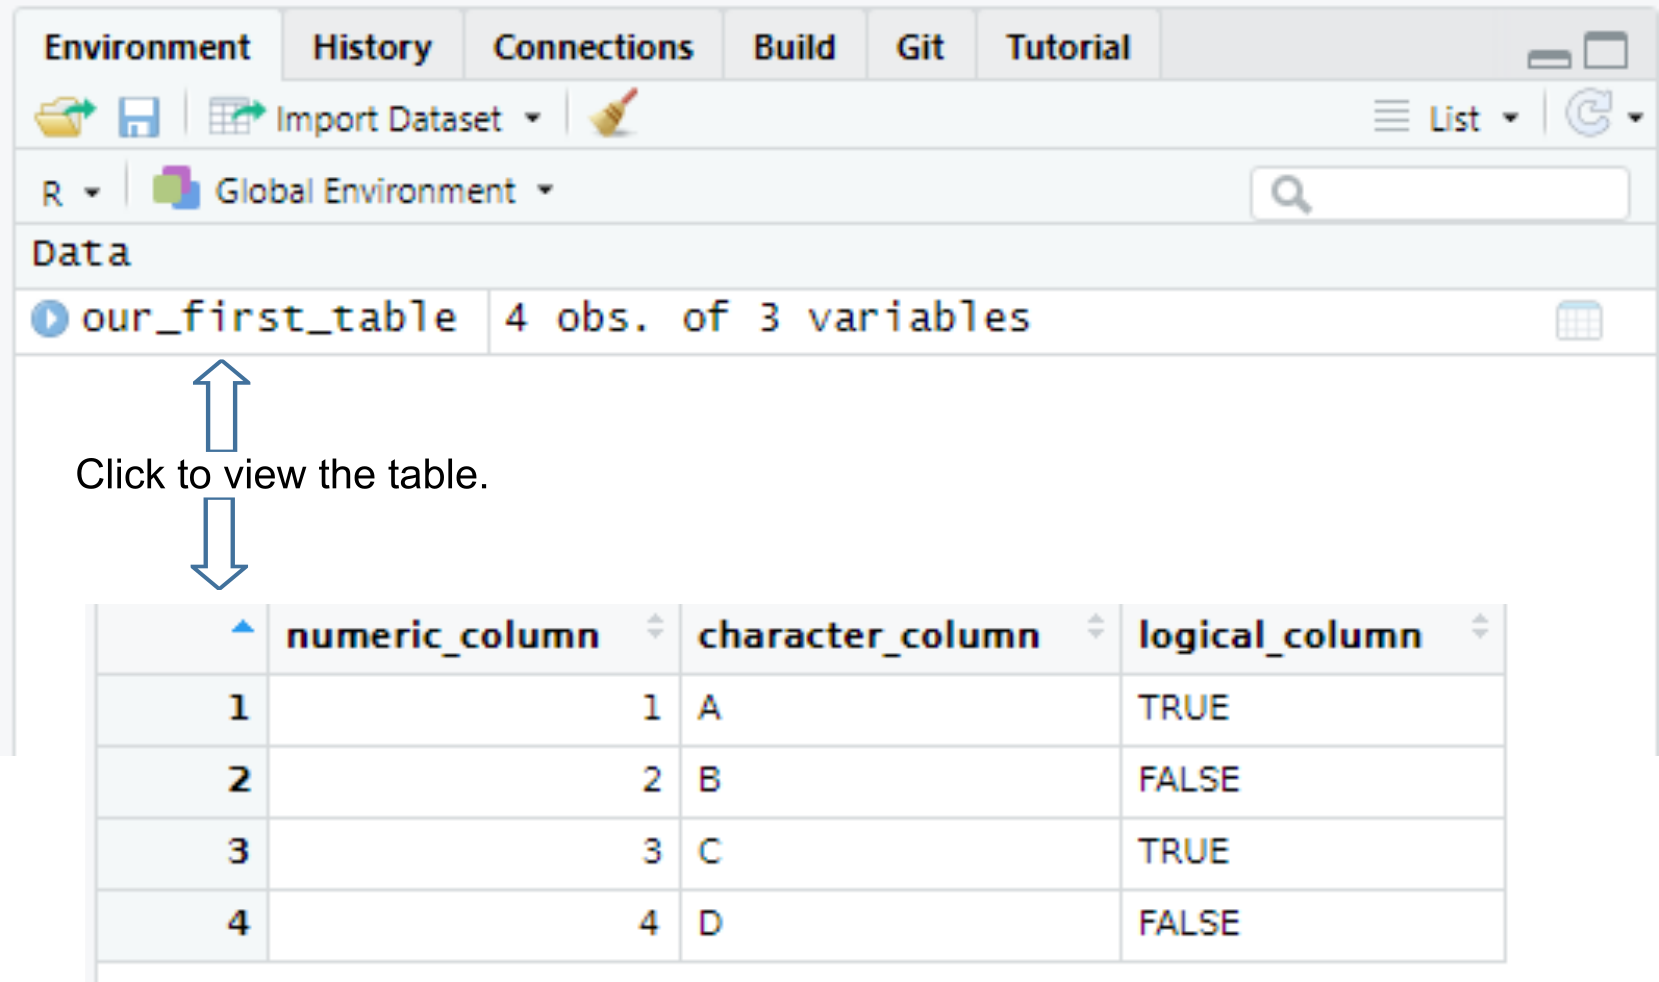
\includegraphics[width=1\linewidth]{images/viewing-table} \end{center}

Do exercise 4.

All columns in a table \textbf{must} have the same number of items (rows). This is similar to the process of \protect\hyperlink{different-length-vectors}{matching vectors' length} that you have learned the last time. However, it works automatically only if length of \emph{all} vectors is a multiple of the longest length. Thus, the example below will work, as the longest vector (\texttt{numeric\_column}) is 6, \texttt{character\_column} length is 3, so it will be repeated twice, and \texttt{logical\_column} length is 2 so it will be repeated thrice.

\begin{Shaded}
\begin{Highlighting}[]
\NormalTok{the\_table }\OtherTok{\textless{}{-}} \FunctionTok{data.frame}\NormalTok{(}\AttributeTok{numeric\_column =} \DecValTok{1}\SpecialCharTok{:}\DecValTok{6}\NormalTok{,                  }\CommentTok{\# length 6 }
                        \AttributeTok{character\_column =} \FunctionTok{c}\NormalTok{(}\StringTok{"A"}\NormalTok{, }\StringTok{"B"}\NormalTok{, }\StringTok{"C"}\NormalTok{),   }\CommentTok{\# length 3}
                        \AttributeTok{logical\_column =} \FunctionTok{c}\NormalTok{(}\ConstantTok{TRUE}\NormalTok{, }\ConstantTok{FALSE}\NormalTok{))       }\CommentTok{\# length 2}
\NormalTok{the\_table}
\end{Highlighting}
\end{Shaded}

\begin{verbatim}
##   numeric_column character_column logical_column
## 1              1                A           TRUE
## 2              2                B          FALSE
## 3              3                C           TRUE
## 4              4                A          FALSE
## 5              5                B           TRUE
## 6              6                C          FALSE
\end{verbatim}

If the simple \emph{multple-of-length} rule does not work, R generates an error (finally!).

\begin{Shaded}
\begin{Highlighting}[]
\CommentTok{\# this will generate an error: arguments imply differing number of rows}
\NormalTok{the\_table }\OtherTok{\textless{}{-}} \FunctionTok{data.frame}\NormalTok{(}\AttributeTok{numeric\_column =} \DecValTok{1}\SpecialCharTok{:}\DecValTok{7}\NormalTok{,                 }\CommentTok{\# length 7}
                        \AttributeTok{character\_column =} \FunctionTok{c}\NormalTok{(}\StringTok{"A"}\NormalTok{, }\StringTok{"B"}\NormalTok{, }\StringTok{"C"}\NormalTok{))  }\CommentTok{\# length 3, cannot be multiplied by an integer to get 7}
\end{Highlighting}
\end{Shaded}

\begin{verbatim}
## Error in data.frame(numeric_column = 1:7, character_column = c("A", "B", : arguments imply differing number of rows: 7, 3
\end{verbatim}

Do exercise 5.

\hypertarget{table-subsetting}{%
\section{Subsetting tables}\label{table-subsetting}}

One way to think about a table as a list of columns (vectors). Hence, both preserving (\texttt{{[}{]}}) and simplifying (\texttt{{[}{[}{]}{]}}) subsetting will work as you would expect returning either a \texttt{data.frame} (\texttt{{[}{]}}) or a \emph{vector} that was a column your were interested in (\texttt{{[}{[}{]}{]}}).

The preserving returns a \emph{table} with \emph{one} column.

\begin{Shaded}
\begin{Highlighting}[]
\NormalTok{our\_first\_table }\OtherTok{\textless{}{-}} \FunctionTok{data.frame}\NormalTok{(}\AttributeTok{numeric\_column =} \FunctionTok{c}\NormalTok{(}\DecValTok{1}\NormalTok{, }\DecValTok{2}\NormalTok{, }\DecValTok{3}\NormalTok{), }
                              \AttributeTok{character\_column =} \FunctionTok{c}\NormalTok{(}\StringTok{"A"}\NormalTok{, }\StringTok{"B"}\NormalTok{, }\StringTok{"C"}\NormalTok{),}
                              \AttributeTok{logical\_column =} \FunctionTok{c}\NormalTok{(}\ConstantTok{TRUE}\NormalTok{, F, T))}

\CommentTok{\# via index}
\NormalTok{our\_first\_table[}\DecValTok{1}\NormalTok{]}
\end{Highlighting}
\end{Shaded}

\begin{verbatim}
##   numeric_column
## 1              1
## 2              2
## 3              3
\end{verbatim}

\begin{Shaded}
\begin{Highlighting}[]
\CommentTok{\# via name }
\NormalTok{our\_first\_table[}\StringTok{\textquotesingle{}numeric\_column\textquotesingle{}}\NormalTok{]}
\end{Highlighting}
\end{Shaded}

\begin{verbatim}
##   numeric_column
## 1              1
## 2              2
## 3              3
\end{verbatim}

\begin{Shaded}
\begin{Highlighting}[]
\CommentTok{\# via slicing}
\NormalTok{our\_first\_table[}\DecValTok{1}\SpecialCharTok{:}\DecValTok{2}\NormalTok{]}
\end{Highlighting}
\end{Shaded}

\begin{verbatim}
##   numeric_column character_column
## 1              1                A
## 2              2                B
## 3              3                C
\end{verbatim}

\begin{center}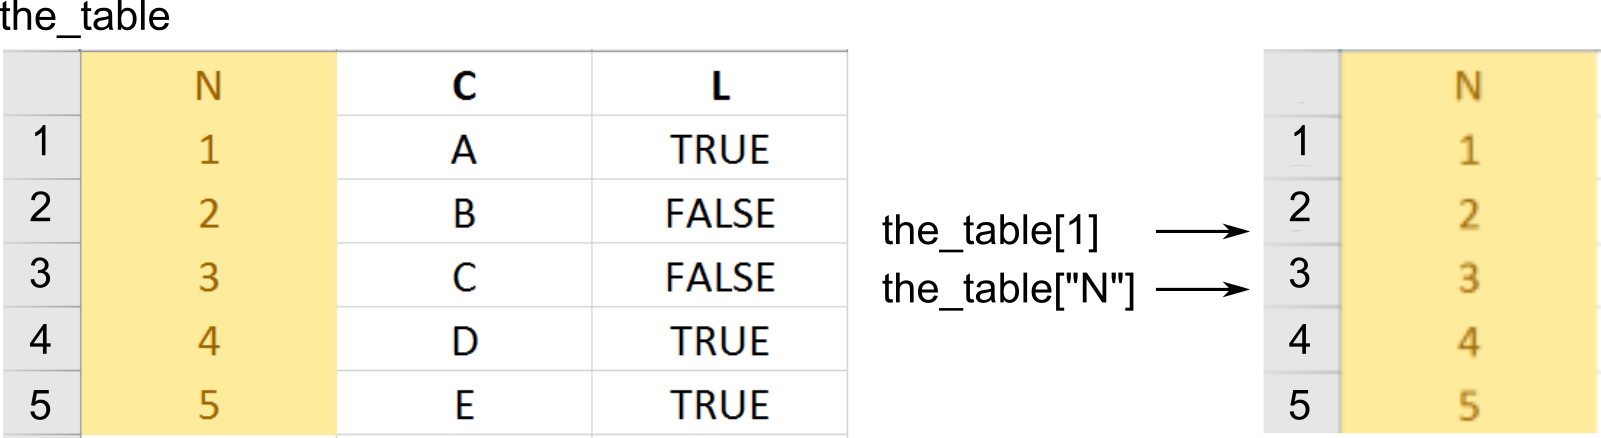
\includegraphics[width=1\linewidth]{images/table-subtable} \end{center}

The simplifying returns a \emph{vector}.

\begin{Shaded}
\begin{Highlighting}[]
\CommentTok{\# via $ notation}
\NormalTok{our\_first\_table}\SpecialCharTok{$}\NormalTok{numeric\_column}
\end{Highlighting}
\end{Shaded}

\begin{verbatim}
## [1] 1 2 3
\end{verbatim}

\begin{Shaded}
\begin{Highlighting}[]
\CommentTok{\# via name and double square brackets}
\NormalTok{our\_first\_table[[}\StringTok{\textquotesingle{}numeric\_column\textquotesingle{}}\NormalTok{]]}
\end{Highlighting}
\end{Shaded}

\begin{verbatim}
## [1] 1 2 3
\end{verbatim}

\begin{Shaded}
\begin{Highlighting}[]
\CommentTok{\# via index and double square brackets}
\NormalTok{our\_first\_table[[}\DecValTok{1}\NormalTok{]]}
\end{Highlighting}
\end{Shaded}

\begin{verbatim}
## [1] 1 2 3
\end{verbatim}

\begin{center}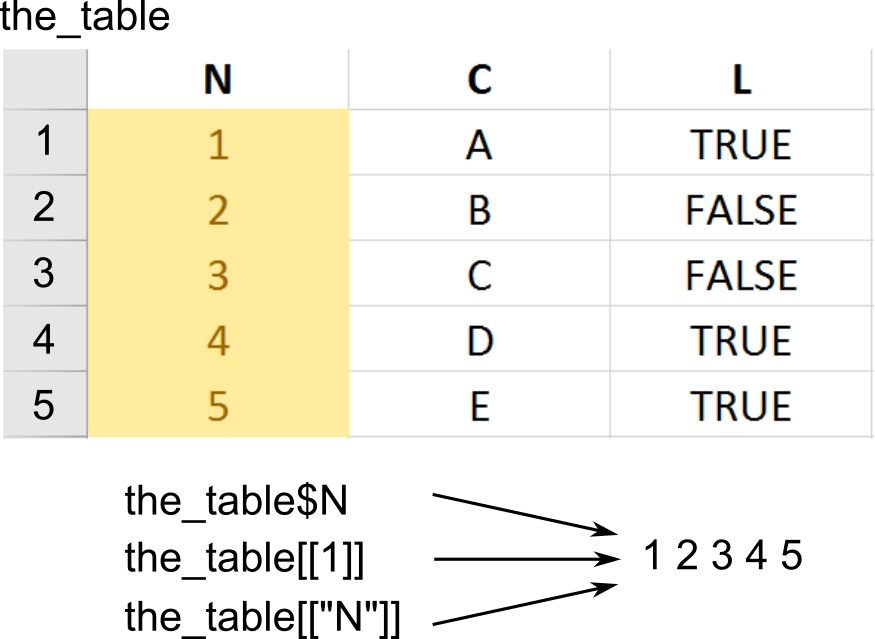
\includegraphics[width=1\linewidth]{images/table-column} \end{center}

The only new thing is that, because tables are two-dimensionsional, you can use preserving subsetting to extract or access a rectangular region within a table. To select a subset rows and columns you write \texttt{table{[}rows,\ columns{]}}. If you omit either rows or columns this implies that you want \emph{all} rows or columns.

\begin{Shaded}
\begin{Highlighting}[]
\CommentTok{\# getting ALL rows for the FIRST column {-}\textgreater{} this gives you a VECTOR}
\NormalTok{our\_first\_table[, }\DecValTok{1}\NormalTok{]}
\end{Highlighting}
\end{Shaded}

\begin{verbatim}
## [1] 1 2 3
\end{verbatim}

\begin{Shaded}
\begin{Highlighting}[]
\CommentTok{\# getting FIRST row for ALL columns {-}\textgreater{} this gives you DATA.FRAME}
\NormalTok{our\_first\_table[}\DecValTok{1}\NormalTok{, ]}
\end{Highlighting}
\end{Shaded}

\begin{verbatim}
##   numeric_column character_column logical_column
## 1              1                A           TRUE
\end{verbatim}

\begin{Shaded}
\begin{Highlighting}[]
\CommentTok{\# ALL rows and ALL columns, equivalent to just writing \textasciigrave{}our\_first\_table\textasciigrave{} or \textasciigrave{}our\_first\_table[]\textasciigrave{}}
\NormalTok{our\_first\_table[,]}
\end{Highlighting}
\end{Shaded}

\begin{verbatim}
##   numeric_column character_column logical_column
## 1              1                A           TRUE
## 2              2                B          FALSE
## 3              3                C           TRUE
\end{verbatim}

\begin{Shaded}
\begin{Highlighting}[]
\CommentTok{\# getting SECOND element of the THIRD column}
\NormalTok{our\_first\_table[}\DecValTok{2}\NormalTok{, }\DecValTok{3}\NormalTok{]}
\end{Highlighting}
\end{Shaded}

\begin{verbatim}
## [1] FALSE
\end{verbatim}

\begin{Shaded}
\begin{Highlighting}[]
\CommentTok{\# getting first two elements of the logical\_column}
\NormalTok{our\_first\_table[}\DecValTok{1}\SpecialCharTok{:}\DecValTok{2}\NormalTok{, }\StringTok{"logical\_column"}\NormalTok{]}
\end{Highlighting}
\end{Shaded}

\begin{verbatim}
## [1]  TRUE FALSE
\end{verbatim}

\begin{center}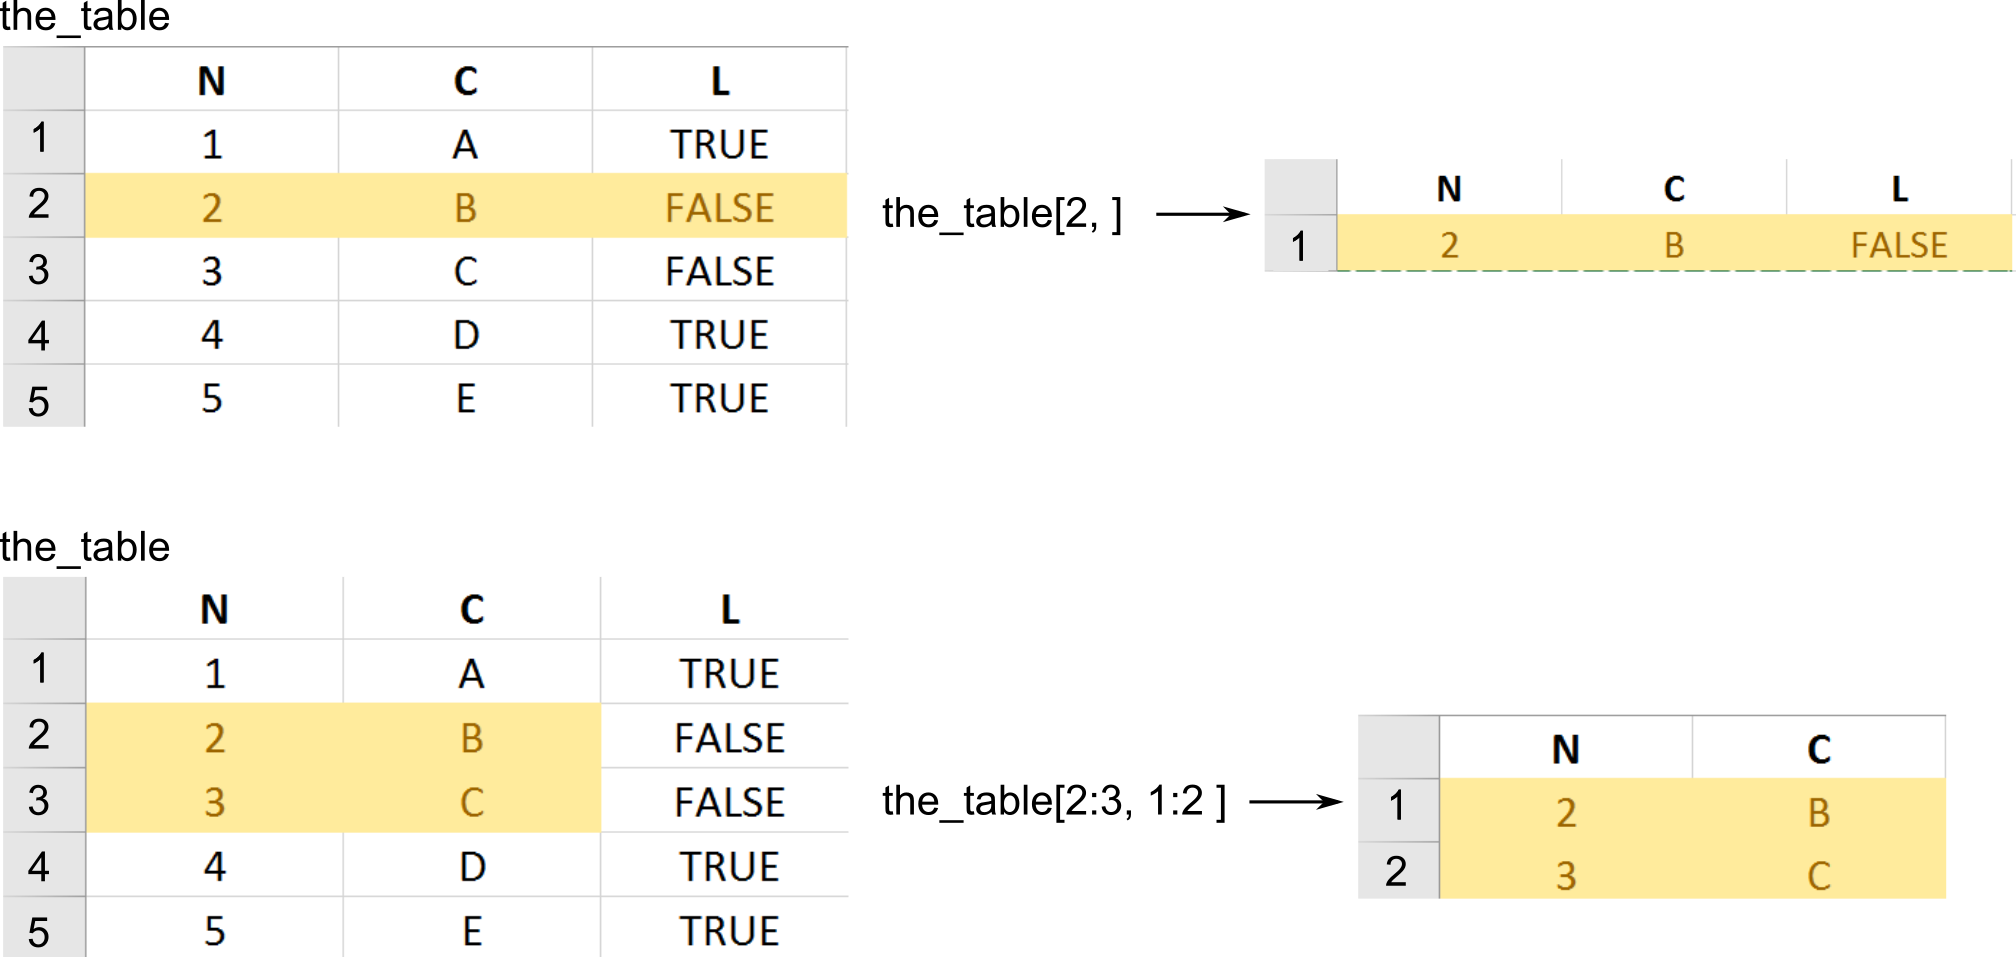
\includegraphics[width=1\linewidth]{images/table-rows-columns} \end{center}

Do exercise 6.

\hypertarget{library}{%
\section{Using libraries}\label{library}}

There is a better way to construct a table but to use it, we need to first import a library that implements it. As with most modern programming languages, the real power of R is not in what comes bundled with it (very little, as a matter of fact) but in community developed libraries that extend it. We already discussed how you \protect\hyperlink{install.packages}{install libraries}. For that you use \href{https://www.rdocumentation.org/packages/base/versions/3.6.2/topics/library}{library()} function (it has a sister function \texttt{require()} but it should be used inside functions and packages not in scripts or notebooks). So, to use \emph{tidyverse} library that you already installed, you simply write

\begin{Shaded}
\begin{Highlighting}[]
\FunctionTok{library}\NormalTok{(tidyverse)}
\CommentTok{\# or}
\FunctionTok{library}\NormalTok{(}\StringTok{"tidyverse"}\NormalTok{)}
\end{Highlighting}
\end{Shaded}

One thing to keep in mind is that if you import two libraries that have a function with same name, the function from the \emph{latter} package will overwrite (mask) the function from the former. You will get a warning but if you miss it, it may be very confusing. My favorite stumbling block are functions \texttt{filter()} from \texttt{dplyr} package (we will use it extensively, as it filters a table by row) and \texttt{filter()} function from \texttt{signal} package (applies a filter to a time-series)\footnote{There is also a filter function is stats library.}. This overwriting of one function by another can lead to very odd looking mistakes. In my case I think that I am using \texttt{dplyr::filter()} and get confused by error messages that I get (they are not really informative). The first time I did this, it took me an hour to figure it out. Here are the warnings I should have paid attention to.

\begin{Shaded}
\begin{Highlighting}[]
\FunctionTok{library}\NormalTok{(signal)}
\end{Highlighting}
\end{Shaded}

\begin{verbatim}
## 
## Attaching package: 'signal'
\end{verbatim}

\begin{verbatim}
## The following objects are masked from 'package:stats':
## 
##     filter, poly
\end{verbatim}

\begin{Shaded}
\begin{Highlighting}[]
\FunctionTok{library}\NormalTok{(dplyr)}
\end{Highlighting}
\end{Shaded}

\begin{verbatim}
## 
## Attaching package: 'dplyr'
\end{verbatim}

\begin{verbatim}
## The following object is masked from 'package:signal':
## 
##     filter
\end{verbatim}

\begin{verbatim}
## The following objects are masked from 'package:stats':
## 
##     filter, lag
\end{verbatim}

\begin{verbatim}
## The following objects are masked from 'package:base':
## 
##     intersect, setdiff, setequal, union
\end{verbatim}

Thus, keep that in mind or, better still, explicitly mention which package the function is coming from via \texttt{library::function()} notation. In this case, you will use the function that you are interested in and need not to worry about other functions with the same name that may conflict with it. In general, it is a good idea to \emph{always} disambiguate function via library but in practice it may make your code hard to read by cluttering it with \texttt{library::} prefixes. Thus, you will need to find a balance between disambiguation and readability.

\begin{Shaded}
\begin{Highlighting}[]
\FunctionTok{library}\NormalTok{(tibble)}

\CommentTok{\# imported from the library into the global environment}
\FunctionTok{print}\NormalTok{(}\FunctionTok{tribble}\NormalTok{(}\SpecialCharTok{\textasciitilde{}}\NormalTok{a, }\DecValTok{1}\NormalTok{))}
\end{Highlighting}
\end{Shaded}

\begin{verbatim}
## # A tibble: 1 x 1
##       a
##   <dbl>
## 1     1
\end{verbatim}

\begin{Shaded}
\begin{Highlighting}[]
\CommentTok{\# used directly from the package}
\NormalTok{tibble}\SpecialCharTok{::}\FunctionTok{tribble}\NormalTok{(}\SpecialCharTok{\textasciitilde{}}\NormalTok{a, }\DecValTok{1}\NormalTok{)}
\end{Highlighting}
\end{Shaded}

\begin{verbatim}
## # A tibble: 1 x 1
##       a
##   <dbl>
## 1     1
\end{verbatim}

When using a notebook (so, in our case, always) put the libraries into \emph{setup} chunk of the notebook. This ensures that your libraries are always initialized, even if you first run some other chunk. Word of advice, keep you library list in alphabetical order. Libraries are very specialized, so you will need quite a few of them for a typical analysis. Keeping them alphabetically organized makes it easier to see whether you imported the required library and whether you need to install a new one.

\hypertarget{tibble}{%
\section{Tibble, a better data.frame}\label{tibble}}

Although the \texttt{data.frame()} function is the default way of creating a table, it is a legacy implementation with numerous shortcomings. Tidyverse implemented its own version of the table called \href{https://tibble.tidyverse.org/}{tibble()} that provides a more rigorous control and more consistent behavior. For example, it allows you to use any symbol in columns names (including spaces), prints out only the beginning of the table rather than entire table, etc. It also gives more warnings. If you try to access a non-existing column both \texttt{data.frame()} and \texttt{tibble()} will return \texttt{NULL} but the former will do it silently, whereas the latter will give you a warning but only if you use the \texttt{\$} notation\footnote{Arbitrariness strikes again! But this also means that \texttt{\$} is safer to use with tibbles but not with data.frames.}.

\begin{Shaded}
\begin{Highlighting}[]
\FunctionTok{library}\NormalTok{(tibble)}

\CommentTok{\# data.frame will return NULL silently}
\NormalTok{df }\OtherTok{\textless{}{-}} \FunctionTok{data.frame}\NormalTok{(}\AttributeTok{b =} \DecValTok{1}\NormalTok{)}
\FunctionTok{print}\NormalTok{(df[[}\StringTok{"A"}\NormalTok{]])}
\end{Highlighting}
\end{Shaded}

\begin{verbatim}
## NULL
\end{verbatim}

\begin{Shaded}
\begin{Highlighting}[]
\CommentTok{\# data.frame will return NULL for a variable that does not exist}

\NormalTok{tbl }\OtherTok{\textless{}{-}} \FunctionTok{tibble}\NormalTok{(}\AttributeTok{b =} \DecValTok{1}\NormalTok{)}
\FunctionTok{print}\NormalTok{(tbl[[}\StringTok{"A"}\NormalTok{]])}
\end{Highlighting}
\end{Shaded}

\begin{verbatim}
## NULL
\end{verbatim}

\begin{Shaded}
\begin{Highlighting}[]
\NormalTok{tbl}\SpecialCharTok{$}\NormalTok{A}
\end{Highlighting}
\end{Shaded}

\begin{verbatim}
## Warning: Unknown or uninitialised column: `A`.
\end{verbatim}

\begin{verbatim}
## NULL
\end{verbatim}

In short, \texttt{tibble()} provides a more robust version of a \texttt{data.frame} but otherwise behaves (mostly) identically to it. Thus, it should be your default choice for a table.

\hypertarget{tribble}{%
\section{Tribble, table from text}\label{tribble}}

The tibble package also provides an easier way of constructing tables via the \href{https://tibble.tidyverse.org/reference/tribble.html}{tribble()} function. Here, you use tilde to specify column names, and then write its content row-by-row.

\begin{Shaded}
\begin{Highlighting}[]
\FunctionTok{tribble}\NormalTok{(}
    \SpecialCharTok{\textasciitilde{}}\NormalTok{x, }\SpecialCharTok{\textasciitilde{}}\NormalTok{y,}
    \DecValTok{1}\NormalTok{,  }\StringTok{"a"}\NormalTok{,}
    \DecValTok{2}\NormalTok{,  }\StringTok{"b"}
\NormalTok{)}
\end{Highlighting}
\end{Shaded}

\begin{verbatim}
## # A tibble: 2 x 2
##       x y    
##   <dbl> <chr>
## 1     1 a    
## 2     2 b
\end{verbatim}

Do exercise 7.

\hypertarget{data}{%
\section{Reading example tables}\label{data}}

One of the great things about R is that most packages come with an example data set that illustrates their function. You can see the list of some of them \href{https://www.rdocumentation.org/packages/datasets}{here}. In case of an example data set, you need to import the library that it is part of and then load them by writing \texttt{data(tablename)}. For example, to use use \texttt{mpg} data on fuel economy from \texttt{ggplot2} package, you need to import the library first, and then call \texttt{data(mpg)}.

\begin{Shaded}
\begin{Highlighting}[]
\FunctionTok{library}\NormalTok{(ggplot2)}
\FunctionTok{data}\NormalTok{(mpg) }\CommentTok{\# this create a "promise" of the data}
\FunctionTok{print}\NormalTok{(mpg) }\CommentTok{\# any action on the promise leads to data appearing in the environment}
\end{Highlighting}
\end{Shaded}

\begin{verbatim}
## # A tibble: 234 x 11
##    manufacturer model      displ  year   cyl trans drv     cty   hwy fl    class
##    <chr>        <chr>      <dbl> <int> <int> <chr> <chr> <int> <int> <chr> <chr>
##  1 audi         a4           1.8  1999     4 auto~ f        18    29 p     comp~
##  2 audi         a4           1.8  1999     4 manu~ f        21    29 p     comp~
##  3 audi         a4           2    2008     4 manu~ f        20    31 p     comp~
##  4 audi         a4           2    2008     4 auto~ f        21    30 p     comp~
##  5 audi         a4           2.8  1999     6 auto~ f        16    26 p     comp~
##  6 audi         a4           2.8  1999     6 manu~ f        18    26 p     comp~
##  7 audi         a4           3.1  2008     6 auto~ f        18    27 p     comp~
##  8 audi         a4 quattro   1.8  1999     4 manu~ 4        18    26 p     comp~
##  9 audi         a4 quattro   1.8  1999     4 auto~ 4        16    25 p     comp~
## 10 audi         a4 quattro   2    2008     4 manu~ 4        20    28 p     comp~
## # ... with 224 more rows
\end{verbatim}

\hypertarget{readr}{%
\section{Reading csv files}\label{readr}}

So far we covered creating a table by hand via \texttt{data.frame()}, \texttt{tibble()}, or \texttt{tribble()} functions and loading an example table from a package via \texttt{data()} function. More commonly, you will need to read a table from an external file. These files can come in many formats because they are generated by different experimental software. Below, you will see how to handle those but my recommendation is to always store your data in a csv (\href{https://en.wikipedia.org/wiki/Comma-separated_values}{Comma-separated values}) files. These are simple plain text files, which means you can open them in any text editor, with each line representing a single row (typically, top row contains column names) with individual columns separated by some symbol or symbols. Typical separators are a comma (hence, the name), a semicolon (this is frequently used in Germany, with comma serving as a decimal point), a tabulator, or even a space symbol. Here is an example of such file

\begin{verbatim}
Participant,Block,Trial,Contrast,Correct
A1,1,1,0.5,TRUE
A1,1,2,1.0,TRUE
A1,1,2,0.05,FALSE
...
\end{verbatim}

that is turned into a table when loaded

\begin{center}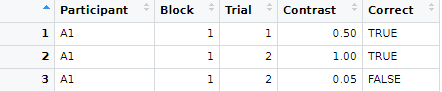
\includegraphics[width=0.7\linewidth]{images/results-csv-table} \end{center}

There are several ways of reading CSV files in R. The default way by using \href{https://stat.ethz.ch/R-manual/R-devel/library/utils/html/read.table.html}{read.csv()} function that has different versions optimized for different combinations of the decimal point and separator symbols, e.g.~\texttt{read.csv2()} assumes a comma for the decimal point and semicolon as a separator. However, a better way is to use \href{https://readr.tidyverse.org/}{readr} library that re-implements same functions. Names of the functions are slightly different with underscore replacing the dot, so \texttt{readr::read\_csv()} is a replacement for \texttt{read.csv()}. These are faster (although it will be noticeable only on large data sets), do not convert text to factor variables (we will talk about factors later but this default conversion by \texttt{read.csv()} can be very confusing), etc.

However, most important difference between \texttt{read.csv()} and \texttt{read\_csv()} is they constraint the content of a CSV file. \texttt{read.csv()} has not assumptions about which columns are in the file and what their value types are. It simply reads them as is, \emph{silently} guessing their type.

\begin{Shaded}
\begin{Highlighting}[]
\NormalTok{results }\OtherTok{\textless{}{-}} \FunctionTok{read.csv}\NormalTok{(}\StringTok{"data/example.csv"}\NormalTok{)}
\NormalTok{results}
\end{Highlighting}
\end{Shaded}

\begin{verbatim}
##   Participant Block Trial Contrast Correct
## 1          A1     1     1     0.50    TRUE
## 2          A1     1     2     1.00    TRUE
## 3          A1     1     2     0.05   FALSE
\end{verbatim}

You can use \texttt{read\_csv()} the same way and it will work the same way but will inform (warn) you about the table structure it deduced.

\begin{Shaded}
\begin{Highlighting}[]
\NormalTok{results }\OtherTok{\textless{}{-}}\NormalTok{ readr}\SpecialCharTok{::}\FunctionTok{read\_csv}\NormalTok{(}\StringTok{"data/example.csv"}\NormalTok{)}
\end{Highlighting}
\end{Shaded}

\begin{verbatim}
## Rows: 3 Columns: 5
\end{verbatim}

\begin{verbatim}
## -- Column specification --------------------------------------------------------
## Delimiter: ","
## chr (1): Participant
## dbl (3): Block, Trial, Contrast
## lgl (1): Correct
\end{verbatim}

\begin{verbatim}
## 
## i Use `spec()` to retrieve the full column specification for this data.
## i Specify the column types or set `show_col_types = FALSE` to quiet this message.
\end{verbatim}

\begin{Shaded}
\begin{Highlighting}[]
\NormalTok{results}
\end{Highlighting}
\end{Shaded}

\begin{verbatim}
## # A tibble: 3 x 5
##   Participant Block Trial Contrast Correct
##   <chr>       <dbl> <dbl>    <dbl> <lgl>  
## 1 A1              1     1     0.5  TRUE   
## 2 A1              1     2     1    TRUE   
## 3 A1              1     2     0.05 FALSE
\end{verbatim}

This annoying \emph{Column specification} print out, which gets even more annoying if you need to read many CSV files, is there for a reason: it wants to annoy you! You can turn it off via \texttt{show\_col\_types\ =\ FALSE} but I strongly recommend against this. Instead, you should specify the column structure yourself via \texttt{col\_types} parameter. The simplest way to do this is via \texttt{spec()} function, as suggested by the printout.

\begin{Shaded}
\begin{Highlighting}[]
\NormalTok{readr}\SpecialCharTok{::}\FunctionTok{spec}\NormalTok{(results)}
\end{Highlighting}
\end{Shaded}

\begin{verbatim}
## cols(
##   Participant = col_character(),
##   Block = col_double(),
##   Trial = col_double(),
##   Contrast = col_double(),
##   Correct = col_logical()
## )
\end{verbatim}

This is a specification that the reader prepared for you. So you can take a look at it, adjust it, if necessary, and copy-paste to the \texttt{read\_csv} call. By default, it suggested \texttt{double} values for \texttt{Block} and \texttt{Trial} but we know they are integers, so we can copy-paste the suggested structure, replace \texttt{col\_double()} with \texttt{col\_integer()} and read the table without a warning.

\begin{Shaded}
\begin{Highlighting}[]
\FunctionTok{library}\NormalTok{(readr)}
\NormalTok{results }\OtherTok{\textless{}{-}} \FunctionTok{read\_csv}\NormalTok{(}\StringTok{"data/example.csv"}\NormalTok{, }
                    \AttributeTok{col\_types =} \FunctionTok{cols}\NormalTok{(}\AttributeTok{Participant =} \FunctionTok{col\_character}\NormalTok{(),}
                                     \AttributeTok{Block =} \FunctionTok{col\_integer}\NormalTok{(), }\CommentTok{\# read\_csv suggested col\_double() but we know better}
                                     \AttributeTok{Trial =} \FunctionTok{col\_integer}\NormalTok{(), }\CommentTok{\# read\_csv suggested col\_double() but we know better}
                                     \AttributeTok{Contrast =} \FunctionTok{col\_double}\NormalTok{(),}
                                     \AttributeTok{Correct =} \FunctionTok{col\_logical}\NormalTok{()))}
\NormalTok{results}
\end{Highlighting}
\end{Shaded}

\begin{verbatim}
## # A tibble: 3 x 5
##   Participant Block Trial Contrast Correct
##   <chr>       <int> <int>    <dbl> <lgl>  
## 1 A1              1     1     0.5  TRUE   
## 2 A1              1     2     1    TRUE   
## 3 A1              1     2     0.05 FALSE
\end{verbatim}

You may feel that this a lot of extra work just to suppress an annoying but, ultimately, harmless warning. Your code will work with or without it, right? Well, \emph{hopefully} it will but you probably want to \emph{know} that it will work not just \emph{hope} for it. Imagine that you accidentally overwrote your experimental data file with data from a different experiment (that happens more often than one would want). You still have \texttt{results.csv} file in your project folder and so the \texttt{read.csv()} will read it as is (it does not know what should be in that file) and your analysis code will fail in some mysterious ways at a much later point (because, remember, if you try to access a column/variable that does not exist in the table, you just get \texttt{NULL} rather than an error). You will eventually trace it back to the wrong data file but that will cost time and nerves. However, if you specify the column structure in \texttt{read\_csv()} it will show a warning, if the file does not match the description. It would warn about wrong column names (\texttt{TheBlock} in the example below) and about wrong type (it does not like \texttt{TRUE}/\texttt{FALSE} in a column it expected to find integers in).

\begin{Shaded}
\begin{Highlighting}[]
\FunctionTok{library}\NormalTok{(readr)}
\NormalTok{results }\OtherTok{\textless{}{-}} \FunctionTok{read\_csv}\NormalTok{(}\StringTok{"data/example.csv"}\NormalTok{, }
                    \AttributeTok{col\_types =} \FunctionTok{cols}\NormalTok{(}\AttributeTok{Participant =} \FunctionTok{col\_character}\NormalTok{(),}
                                     \AttributeTok{TheBlock =} \FunctionTok{col\_integer}\NormalTok{(), }\CommentTok{\# read\_csv suggested col\_double() but we know better}
                                     \AttributeTok{Trial =} \FunctionTok{col\_integer}\NormalTok{(), }\CommentTok{\# read\_csv suggested col\_double() but we know better}
                                     \AttributeTok{Contrast =} \FunctionTok{col\_double}\NormalTok{(),}
                                     \AttributeTok{Correct =} \FunctionTok{col\_integer}\NormalTok{()))}
\end{Highlighting}
\end{Shaded}

\begin{verbatim}
## Warning: The following named parsers don't match the column names: TheBlock
\end{verbatim}

Personally, I would prefer for \texttt{read\_csv()} to loudly fail with an error in cases like these but having a nice red warning is already very helpful to quickly detect the problem with your data (and if your data is wrong, your whole analysis is meaningless). Thus, \emph{always} use \texttt{read\_} rather than \texttt{read.} functions and \emph{always} specify the table structure. The lazy, and my preferred, way to do it, is to first read the file without specifying the structure and copy-paste-edit the warning column-specification message into the code adjusting as necessary.

Do exercise 8, you need \href{data/face_rank.csv}{face\_rank.csv} file for it. Download it and place it in the project folder. \emph{Warning}, if you use Chrome or any Chromium-based browsers like MS Edge, Opera, etc. they might, for some odd reason, automatically \emph{rename it} into \emph{face\_rank.xls} during the download. Just rename it back to \emph{face\_rank.csv}, because the file itself is not converted to an Excel, it is only the extension that gets changed (why? No idea, ask Google!).

\hypertarget{readxl}{%
\section{Reading Excel files}\label{readxl}}

There are several libraries that allow you to read Excel files directly. My personal preference is \href{https://readxl.tidyverse.org/}{readxl} package, which is part of the Tidyverse. Warning, it will be installed as part of the Tidyverse (i.e., when you typed \texttt{install.packages(tidyverse)}) but you still need to import it explicitly via \texttt{library(readxl)}. Because an Excel file has many sheets, by default the \texttt{read\_excel()} function reads the \emph{first} sheet but you can specify it via a \texttt{sheet} parameter using its index \texttt{read\_excel("my\_excel\_file.xls",\ sheet=2)} or name \texttt{read\_excel("my\_excel\_file.xls",\ sheet="addendum")}.

Do exercise 9, you need \href{data/face_rank.xlsx}{face\_rank.xlsx} file for it.

You can read about further options at the package's website but I would generally discourage you from using Excel for your work and, definitely, for your data analysis. Because, you see, Excel is very smart and it can figure out the \emph{true} meaning and type of columns by itself. The fact that you might disagree is your problem. Excel knows what is best for you. The easiest way to screw a CSV file up (at least in Germany) is to open it in Excel and immediately save it. The file name will remain the same but Excel will ``adjust'' the content as it feels is better for you (you don't need to be consulted with). If you think I am exaggerating, read this \href{https://www.theverge.com/2020/8/6/21355674/human-genes-rename-microsoft-excel-misreading-dates}{article} at The Verge on how Excel messed up thousands of human genome data tables by turning some values into dates (because why not?). So now the entire community is \emph{renaming} some genes because it is easier to waste literally thousands of man-hours on that than to fix Excel. In short, friends don't let friends use Excel.

\hypertarget{reading-files-from-other-programs}{%
\section{Reading files from other programs}\label{reading-files-from-other-programs}}

World is a very diverse place, so you are likely to encounter a wide range of data files generated by Matlab, SPSS, SAS, etc. There are two ways to import the data. First, that I would recommend, use the original program (Matlab, SPSS, SAS, etc.) to export data as a CSV file. Every program can read and write CSV, so it a good common ground. Moreover, this is a simple format with no embedded formulas (as in Excel), service structures, etc. Finally, if you store your data in CSV, you do not need a special program to work with it. In short, unless you have a good reason, store your data in CSV files.

However, sometimes you have a file but you do not have the program (Matlab, SPSS, SAS, etc.). The second way is to use various R libaries, starting with \href{https://www.rdocumentation.org/packages/foreign}{foreign}, which can handle most typical cases, e.g., SPSS, SAS, State, or Minitab. The problem here is that all programs differ in the internal file formats and what exactly is included. For example, when importing from an SPSS sav-file via \href{https://www.rdocumentation.org/packages/foreign/versions/0.8-80/topics/read.spss}{read.spss} you will get a list with various components rather than a table (\texttt{data.frame}). You can force the function to convert everything to a single table via \texttt{to.data.frame=TRUE} option but you may lose some information. Bottom line, you need to be extra careful when importing from other formats and the safest way is to ensure complete and full export of the data to a CSV from the original program.

\hypertarget{rds}{%
\section{Writing and reading a single object}\label{rds}}

\hypertarget{wrap-up-1}{%
\section{Wrap up}\label{wrap-up-1}}

We have started with vectors and now extended them to tables. Next time, we will look at how to visualize the data using The Grammar of Graphics approach.

\hypertarget{functions}{%
\chapter{Functions! Functions everywhere!}\label{functions}}

In this chapter you will learn about \emph{functions} in R, as they are the second most important concept in R and are everywhere (just like vectors and lists). You will also learn how to \emph{pipe} your computation through series of functions without creating a mess of temporary variables or nested calls. Don't forget to download the \href{notebooks/Seminar\%2004\%20-\%20functions.Rmd}{notebook}.

\hypertarget{functions-1}{%
\section{Functions}\label{functions-1}}

In the previous chapters, you have learned that you can store information in variables --- ``boxes with slots'' --- as \protect\hyperlink{vectors}{vectors} or as \protect\hyperlink{tables}{tables} (bundles of vectors of equal length). To use these stored values for computation you need functions. In programming, function is an \emph{isolated} code that receives some input, performs some action on it, and, optionally, returns a value\footnote{Function that does not return a value, probably, generates its output to a console, external file, etc. There is little point in running a function that does not affect the world.}. The concept of functions comes from mathematics, so it might be easier to understand them using R implementation of mathematical functions. For example, you may remember a sinus function from trigonometry. It is typically abbreviated as \texttt{sin}, it takes a numeric value of angle (in radians) as its \emph{input} and returns (this is its \emph{output}) a corresponding value between -1 and 1: \(sin(0) = 0\), \(sin(\pi/2) = 1\), etc.

\begin{center}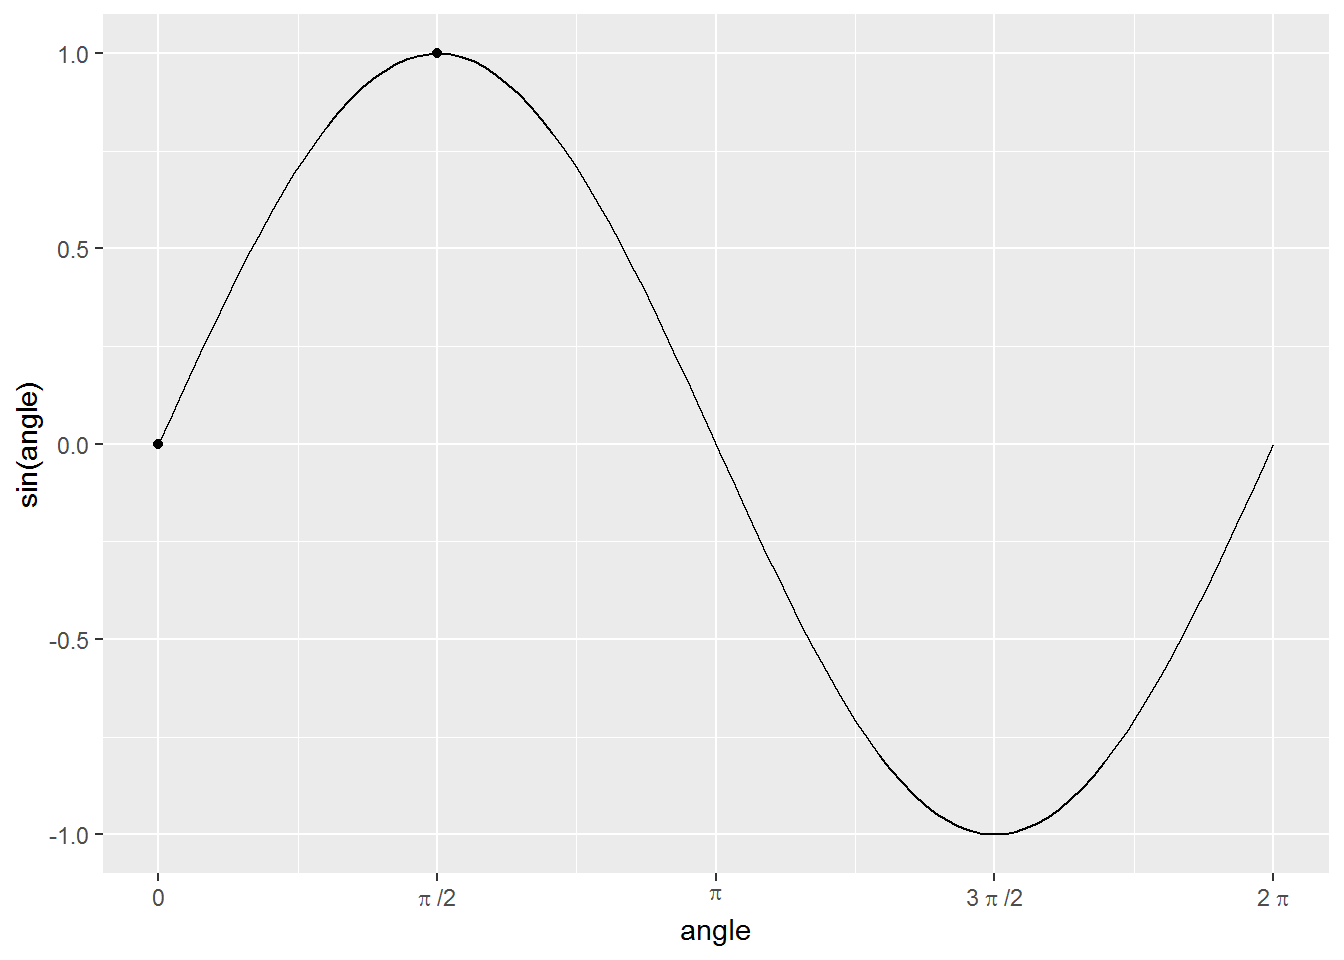
\includegraphics{data-analysis-using-r-for-psychology_files/figure-latex/unnamed-chunk-100-1} \end{center}

In R, you write a function using the following template

\begin{Shaded}
\begin{Highlighting}[]
\NormalTok{name\_of\_the\_function }\OtherTok{\textless{}{-}} \ControlFlowTok{function}\NormalTok{(parameter1, parameter2, parameter3, ...)\{}
\NormalTok{  ...some code that computes the value...}
  \FunctionTok{return}\NormalTok{(value);}
\NormalTok{\}}
\end{Highlighting}
\end{Shaded}

A \texttt{sin} function with a single parameter \texttt{angle} would look something like this

\begin{Shaded}
\begin{Highlighting}[]
\NormalTok{sin }\OtherTok{\textless{}{-}} \ControlFlowTok{function}\NormalTok{(angle)\{}
\NormalTok{  ...some math that actually computes sinus of angle using value of angle parameter ...}
  \FunctionTok{return}\NormalTok{(sin\_of\_angle);}
\NormalTok{\}}
\end{Highlighting}
\end{Shaded}

Once we have the function, we can use it by \emph{calling} it. You simply write \texttt{sin(0)}\footnote{I've cheated here by using R implementation of \href{https://stat.ethz.ch/R-manual/R-devel/library/base/html/Trig.html}{sin()}.} and get the answer!

\begin{Shaded}
\begin{Highlighting}[]
\FunctionTok{sin}\NormalTok{(}\DecValTok{0}\NormalTok{)}
\end{Highlighting}
\end{Shaded}

\begin{verbatim}
## [1] 0
\end{verbatim}

As you hopefully remember, all simple values are vectors, so instead of using a scalar \texttt{0} (merely a vector of length of one) you can write and apply this function to (compute sinus for) every element in the vector.

\begin{Shaded}
\begin{Highlighting}[]
\FunctionTok{sin}\NormalTok{(}\FunctionTok{seq}\NormalTok{(}\DecValTok{0}\NormalTok{, }\FloatTok{3.141593}\NormalTok{, }\AttributeTok{length.out =} \DecValTok{5}\NormalTok{))}
\end{Highlighting}
\end{Shaded}

\begin{verbatim}
## [1]  0.000000e+00  7.071068e-01  1.000000e+00  7.071066e-01 -3.464102e-07
\end{verbatim}

You can think of functions parameters as local function variables those values are set before the function is called. A function can have any number of parameters, including zero\footnote{This, probably, means that the function always does the same thing or a random thing and you cannot influence this.}, one, or many parameters. For example, an arctangent \href{https://stat.ethz.ch/R-manual/R-devel/library/base/html/Trig.html}{atan2} function takes 2D coordinates (\texttt{y} and \texttt{x}, in that order!) and returns a corresponding angle in \emph{radians}.

\begin{Shaded}
\begin{Highlighting}[]
\FunctionTok{atan2}\NormalTok{(}\FunctionTok{c}\NormalTok{(}\DecValTok{0}\NormalTok{, }\DecValTok{1}\NormalTok{), }\FunctionTok{c}\NormalTok{(}\DecValTok{1}\NormalTok{, }\DecValTok{1}\NormalTok{))}
\end{Highlighting}
\end{Shaded}

\begin{verbatim}
## [1] 0.0000000 0.7853982
\end{verbatim}

A definition of this function would look something like this

\begin{Shaded}
\begin{Highlighting}[]
\NormalTok{atan2 }\OtherTok{\textless{}{-}} \ControlFlowTok{function}\NormalTok{(y, x)\{}
\NormalTok{  ...magic that uses values of y and x parameters...}
\NormalTok{  ...to compute the angle\_in\_rad value...}
  \FunctionTok{return}\NormalTok{(angle\_in\_rad);}
\NormalTok{\}}
\end{Highlighting}
\end{Shaded}

Do exercise 1.

\hypertarget{writing-a-function}{%
\section{Writing a function}\label{writing-a-function}}

Let us start practicing computing things in R and writing functions at the same time. We will begin by implementing a very simple function that doubles a given number. We will write this function in steps. First, think about how you would name\footnote{\texttt{double\_or\_nothing}?} this function (meaningful names are your path to readable and re-usable code!) and how many parameters it will have. Write the definition of the function without any code inside of wiggly brackets (so, no actual computation or a return statement at the end of it).

Do exercise 2.1

Next, think about the code that would \emph{double-the-value} based on the parameter. This is the code that will eventually go inside the wiggly brackets. Write that code (just the code, without the bits from exercise 2.1) in exercise 2.2 and test it by creating a variable with the same name as your parameter inside the function. E.g., if my parameter name is \texttt{the\_number}, I would test it as

\begin{Shaded}
\begin{Highlighting}[]
\NormalTok{the\_number }\OtherTok{\textless{}{-}} \DecValTok{1}
\NormalTok{...my code to double the value usign the\_number variable...}
\end{Highlighting}
\end{Shaded}

Do exercise 2.2

By now you have your formal function definition (exercise 2.1) and the actual code that should go inside (exercise 2.2). Now, we just need to combine them by putting the code inside the function and \emph{returning} the value. You can do this two ways:

\begin{enumerate}
\def\labelenumi{\arabic{enumi})}
\tightlist
\item
  you can store the results of the computation in a separate local variable and then return that variable,
\item
  return the results of the computation directly
\end{enumerate}

\begin{verbatim}
# 1) first store in a local variable, then return it
  result <- ...some computation you perform...
  return(result);

# 2) returning results of computation directly
  return(...some computation you perform...);
\end{verbatim}

Do it \emph{both} ways in exercises 2.3 and 2.4. Call the function using different inputs to test that it works.

Do exercise 2.3 and 2.4

More practice is always good, so write a function that converts an angle in \emph{degrees} to \emph{radians}. The formula\footnote{Hint: \href{https://stat.ethz.ch/R-manual/R-devel/library/base/html/Constants.html}{Constants}} is
\[rad = \frac{deg \cdot \pi}{180}\]
Decide whether you want to a have an intermediate local variable inside the function or to return the results of the computation directly.

Do exercise 3

\hypertarget{scopes-global-versus-local-variables}{%
\section{Scopes: Global versus Local variables}\label{scopes-global-versus-local-variables}}

I suggested that you use a variable to store the results of double-it-up computation before returning it. But why did I call it \emph{local?} This is because each function has it own \emph{scope} (environment with variables and functions) that is (mostly) independent from the scope of the global script. Unfortunately, environment scopes in R are different and more complicated than those in other programming languages, such Python, C/C++, or Java, so always pay attention and be careful in the future.

The \emph{global} scope/environment is the environment for the code \emph{outside} of functions. All \emph{global} variables and functions, the ones that you define in the code \emph{outside} of functions (typing in the console, running scripts, running chunks of code in notebooks, etc.), live where. You can see what you have in the global scope at any time by looking at \emph{Environment} tab (note the \emph{Global Environment} tag).

\begin{center}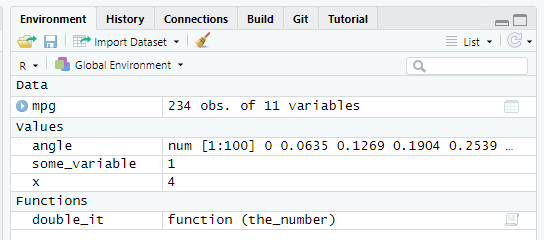
\includegraphics[width=0.7\linewidth]{images/environment-tab} \end{center}

In my case, it has one table (\texttt{mpg}, all tables go under \emph{Data}), three vectors (\texttt{angle}, \texttt{some\_variable}, and \texttt{x}, all vectors go under \texttt{Values}), and an example function from exercise \#2 that I created (\texttt{double\_it}, all functions go under \emph{Functions}, makes sense). However, it has no access to parameters of the functions and variables that you define inside these function. When you run a function, it has it own scope/environment that includes \emph{parameters} of the function (e.g., \texttt{the\_number} for my \texttt{double\_it} function and the value it was assigned during the call), any \emph{local} variables you create inside that function (e.g., \texttt{result\ \textless{}-\ ...some\ computation\ you\ perform...} creates such local variable), and a \textbf{copy(!)} of all \emph{global} variables\footnote{You can write to a parent (e.g., global) environment from inside the function via \href{https://stat.ethz.ch/R-manual/R-devel/library/base/html/assignOps.html}{\textless\textless-} operator. However, this should be your last resort, as it makes the code brittle and harder to understand and debug, because if depends not only on local things but on global variables that may or may not be where at any given moment.}. In the code below, take a look at the comments that specify the accessibility of variables between global script and functions (ignore \href{https://glue.tidyverse.org/reference/glue.html}{glue} for a moment, it \emph{glues} a variable's value into the text, so I use it to make printouts easier to trace)\footnote{These rules --- a \textbf{copy} of a global scope is accessible inside a function but function scope is inaccessible from outside --- should be how \emph{you} write your code. However, R's motto is ``anything is possible'', so be aware that \emph{other people} may not respect these rules. This should not be an issue most of the time but if you are curious how R can let you break all rules of good responsible programming and do totally crazy things, read \href{https://adv-r.hadley.nz/}{Advanced R} book by Hadley Wickham. However, it is really \textbf{advanced}, aimed primarily at programmers who develop R and packages, not at scientists who use them.}

\begin{Shaded}
\begin{Highlighting}[]
\CommentTok{\# this is a GLOBAL variable}
\NormalTok{global\_variable }\OtherTok{\textless{}{-}} \DecValTok{1}

\NormalTok{i\_am\_test\_function }\OtherTok{\textless{}{-}} \ControlFlowTok{function}\NormalTok{(parameter)\{}
  \CommentTok{\# parameter live is a local function scope}
  \CommentTok{\# its values are set when you call a function}
  \FunctionTok{print}\NormalTok{(}\FunctionTok{glue}\NormalTok{(}\StringTok{"  parameter inside the function: \{parameter\}"}\NormalTok{))}
  
  \CommentTok{\# local variable created inside the function}
  \CommentTok{\# it is invisible from outside}
\NormalTok{  local\_variable }\OtherTok{\textless{}{-}} \DecValTok{2}
  \FunctionTok{print}\NormalTok{(}\FunctionTok{glue}\NormalTok{(}\StringTok{"  local\_variable inside the function: \{local\_variable\}"}\NormalTok{))}
  
  \CommentTok{\# here, a\_global\_variable is a LOCAL COPY of the the global variable}
  \CommentTok{\# of the same name. You can use this COPY}
  \FunctionTok{print}\NormalTok{(}\FunctionTok{glue}\NormalTok{(}\StringTok{"  COPY of global\_variable inside the function: \{global\_variable\}"}\NormalTok{))}
  
  \CommentTok{\# you can modify the LOCAL COPY but that won\textquotesingle{}t affect the original!}
\NormalTok{  global\_variable }\OtherTok{\textless{}{-}} \DecValTok{3}
  \FunctionTok{print}\NormalTok{(}\FunctionTok{glue}\NormalTok{(}\StringTok{"  CHANGED COPY of global\_variable inside the function: \{global\_variable\}"}\NormalTok{))}
\NormalTok{\}}

\FunctionTok{print}\NormalTok{(}\FunctionTok{glue}\NormalTok{(}\StringTok{"global\_variable before the function call: \{global\_variable\}"}\NormalTok{))}
\end{Highlighting}
\end{Shaded}

\begin{verbatim}
## global_variable before the function call: 1
\end{verbatim}

\begin{Shaded}
\begin{Highlighting}[]
\FunctionTok{i\_am\_test\_function}\NormalTok{(}\DecValTok{5}\NormalTok{)}
\end{Highlighting}
\end{Shaded}

\begin{verbatim}
##   parameter inside the function: 5
##   local_variable inside the function: 2
##   COPY of global_variable inside the function: 1
##   CHANGED COPY of global_variable inside the function: 3
\end{verbatim}

\begin{Shaded}
\begin{Highlighting}[]
\CommentTok{\# the variable outside is unchanged because we modify its COPY, not the variable itself}
\FunctionTok{print}\NormalTok{(}\FunctionTok{glue}\NormalTok{(}\StringTok{"UNCHANGED global\_variable after the function call: \{global\_variable\}"}\NormalTok{))}
\end{Highlighting}
\end{Shaded}

\begin{verbatim}
## UNCHANGED global_variable after the function call: 1
\end{verbatim}

Do exercise 4 to build understanding of scopes.

\hypertarget{function-with-two-parameters}{%
\section{Function with two parameters}\label{function-with-two-parameters}}

Let us write a function that takes \emph{two} parameters --- \texttt{x} and \texttt{y} --- and computes \emph{radius} (distance from \texttt{(0,0)} to \texttt{(x,\ y)})\footnote{This function is complementary to \texttt{atan2()}, as two of them allow transformation of coordinates from Cartesian to polar coordinate system}. The formula is
\[R = \sqrt{x^2 + y^2}\]
This is very similar to exercises 2 and 3, with number of parameters being the only difference.

Do exercise 5.

\hypertarget{table-as-a-parameter}{%
\section{Table as a parameter}\label{table-as-a-parameter}}

So far, we only passed vectors (a.k.a. values) to functions but you can pass any object including tables\footnote{And even functions themselves, not just what they computed! This is part of \emph{functional programming} you will learn about later.}. Let us use \href{https://ggplot2.tidyverse.org/reference/mpg.html}{mpg} table from the \emph{ggplot2} package. Write a function that takes a table as a \emph{parameter}. This mean that the function should not assume that a table with this name exists in the global environment. Do not use \texttt{mpg} as a parameter name (makes it confusing and hard to understand which table global or local you actually mean), call it something else\footnote{I tend to use \texttt{df}, if it is reasonably easy to deduce what sort of \texttt{data.frame} I mean.}. The function should compute and return average miles-per-gallon efficiency based on city \texttt{cty} and highway \texttt{hwy} test cycles. Do it in \emph{two} ways. First, compute and return \emph{a vector} based on the table passed as parameter. Second, do the same computation but add the result \emph{to the table that function received as a parameter} (call the new column \texttt{avg\_mpg}) and return the entire table (remember, modifying table is not enough, as you are working \emph{on a copy}).

Do exercise 6.

Let us write another function that computes \href{https://stat.ethz.ch/R-manual/R-devel/library/base/html/mean.html}{mean} efficiency for a particular cycle, either city or highway. For this, the function will take \emph{two} parameters: 1) the table itself and 2) a string (text variable) with the name of the column. Then, you use it to access the column via simplifying \texttt{{[}{[}{]}{]}} \protect\hyperlink{subsetting}{subsetting}. To summarize, your function takes 1) a table and 2) a string with a column name and returns a single number (mean for the specified column). E.g.

\begin{Shaded}
\begin{Highlighting}[]
\FunctionTok{average\_efficiency}\NormalTok{(mpg, }\StringTok{"cty"}\NormalTok{) }\CommentTok{\# should return 16.85897}
\end{Highlighting}
\end{Shaded}

Do exercise 7.

\hypertarget{named-versus-positional-arguments}{%
\section{Named versus positional arguments}\label{named-versus-positional-arguments}}

Remember than we talked about the \protect\hyperlink{assignment-statement}{assignment statement}, I noted that you should always use \href{https://stat.ethz.ch/R-manual/R-devel/library/base/html/assignOps.html}{\textless-} operator for assignments but warned you that you will encounter an alternative \texttt{=} operator when we will use functions. You also may have notice me using it, for example, in \texttt{seq(0,\ 2*pi,\ length.out\ =\ 100)}. Why did I use name for the third parameter and not the other two? Why did I have to use \texttt{length.out=} at all? This is because in R you can pass arguments by \emph{position} (first two arguments in that example) or by \emph{name} (that would be \texttt{length.out=}).

Then you pass arguments by \emph{position}, values are put into corresponding arguments in the order you supplied them in. I.e., the first value goes into the first parameter, the second into the second etc. Then you specify arguments by \emph{name}, you explicitly state which argument gets which value \texttt{arg\ =\ value}. Here, the exact order does not matter and you can put arguments in the order you need (i.,e., an order that makes understanding the code easier). You can also mix these two ways and, R being R, you can really mix them interleaving positional and named arguments any way you like\footnote{That being a case, never use named argument before positional ones. Each time you use a named argument, its position is taken out and that \emph{changes} position index for remaining positional arguments. This is an almost certain way to put a value into a wrong parameter and, at the same time, create an error that is really hard to find.}. Despite all the flexibility that R gives you to confuse yourself and others, use only all-positional-followed-by-all-named-arguments order, e.g., \texttt{seq(0,\ 2*pi,\ length.out\ =\ 100)}.

When should you use which? That depends solely on which way is clearer or possible. For a single parameter or widely used mathematical functions, like \href{https://stat.ethz.ch/R-manual/R-devel/library/base/html/mean.html}{mean} or \href{https://stat.ethz.ch/R-manual/R-devel/library/base/html/Trig.html}{sin} there is little point in using names (particularly, because the only argument is named \texttt{x}). At the same time, I \emph{always} use named parameters for \href{https://stat.ethz.ch/R-manual/R-devel/library/base/html/Trig.html}{atan2} simply because I am never 100\% sure about the order (i.e., \texttt{x} followed by \texttt{y} occurs far more often). At the same time, formulas for statistical models in R have a very specific look and are typically a first argument, so it is probably redundant to specify that \texttt{formula\ =\ y\ \textasciitilde{}\ x}.Returning to the \href{https://stat.ethz.ch/R-manual/R-devel/library/base/html/seq.html}{seq()} function, the \texttt{length.out} is actually its \emph{fourth} argument with \texttt{by} (an alternative way to define how many values you will get in the sequence) being third. But because both parameters define, essentially, the same thing, it is \emph{impossible} to specify \texttt{length.out} using positional arguments only. Finally, if a function has more than a couple of parameters, it is probably a good idea to use named arguments. In short, use you own better judgement on whatever makes understanding the code easier.

Do exercise 8.

\hypertarget{default-values}{%
\section{Default values}\label{default-values}}

When you write a function, you can combine simplicity of its use with flexibility via \emph{default values}. I.e., \emph{some} parameters can have sensible or commonly used values but, if desired, a user can specify their own values to modify functions behavior. For example, function \href{https://stat.ethz.ch/R-manual/R-devel/library/base/html/mean.html}{mean} has \emph{three} parameters. You always need to specify the first one (\texttt{x}, a vector of values you are computing the mean of). But you can also specify trimming via \texttt{trim} and whether it should ignore \texttt{NA} via \texttt{na.rm}\footnote{If you do not ignore \texttt{NA} then the mean of a vector with at least one \texttt{NA} in it is \texttt{NA} as well}. By default, you do not trim (\texttt{trim\ =\ 0}) and do not ignore \texttt{NA} (\texttt{na.rm\ =\ FALSE}). These defaults are sensible as they produce a most typically expected behavior. At the same time their existence means that you can fine-tune your mean computation the way you require.

When writing you own function, you simply specify the default values when you define an argument. E.g., here, the second parameter \texttt{r}, the radius, has a default value of 1, so you can only specify the direction of the vector to compute (x, y) coordinates for a (default) \emph{unit} vector.

\begin{Shaded}
\begin{Highlighting}[]
\NormalTok{polar\_to\_cartesian }\OtherTok{\textless{}{-}} \ControlFlowTok{function}\NormalTok{(angle, }\AttributeTok{r=}\DecValTok{1}\NormalTok{) \{}
  \CommentTok{\# ...}
\NormalTok{\}}
\end{Highlighting}
\end{Shaded}

Do exercise 9.

\hypertarget{nested-calls}{%
\section{Nested calls}\label{nested-calls}}

What if you need to call several functions in a single chain to compute a result? Think about the function from exercise \#3 that converts degree to radians. Its most likely usage scenario is to convert degrees to radians and use that to compute sinus (or some other trigonometric function). There are different ways you can do this. For example, you can store the angle in radians in some temporary variable (e.g., \texttt{angle\_in\_radians}) and then pass it to sinus function during the next call.

\begin{Shaded}
\begin{Highlighting}[]
\NormalTok{angle\_in\_radians }\OtherTok{\textless{}{-}} \FunctionTok{deg2rad}\NormalTok{(}\DecValTok{90}\NormalTok{) }\CommentTok{\# function returns 1.570796, this value is stored in angle\_in\_radians}
\FunctionTok{sin}\NormalTok{(angle\_in\_radians) }\CommentTok{\# returns 1}
\end{Highlighting}
\end{Shaded}

Alternatively, you can use the value returned by \texttt{deg2rad()} \emph{directly} as a parameter for function \texttt{sin()}

\begin{Shaded}
\begin{Highlighting}[]
\FunctionTok{sin}\NormalTok{(}\FunctionTok{deg2rad}\NormalTok{(}\DecValTok{90}\NormalTok{)) }\CommentTok{\# returns 1}
\end{Highlighting}
\end{Shaded}

In this case, the computation proceeds in an \emph{inside-out} order: The innermost function gets computed first, the function that uses its return value is next, etc. Kind of like assembling a Russian doll: you start with an innermost, put it inside a slightly bigger one, now take that one put it inside the next, etc. Nesting means that you do not need to pollute you memory with temporary variables\footnote{The worst case scenario is when you use same \texttt{temp} variable for things like that, forget to initialize / change its value properly at some point, spend half-a-day trying to understand why your code does not generate an error but results don't make sense.} and make your code more expressive as nesting explicitly informs the reader that intermediate results are of no value by themselves and are not saved for later use.

Do exercise 10.

\hypertarget{pipe}{%
\section{Piping}\label{pipe}}

Although nesting is better than having tons of intermediate variables, lots of nesting can be mightily confusing. Tidyverse has an alternative way to chain or, in Tidyverse-speak, \href{https://magrittr.tidyverse.org/reference/pipe.html}{pipe} a computation through a series of function calls. The magic operator is \texttt{\%\textgreater{}\%} (that's the pipe) and here is how it transforms our nested call

\begin{Shaded}
\begin{Highlighting}[]
\FunctionTok{sin}\NormalTok{(}\FunctionTok{deg2rad}\NormalTok{(}\DecValTok{90}\NormalTok{)) }\CommentTok{\# returns 1}

\FunctionTok{deg2rad}\NormalTok{(}\DecValTok{90}\NormalTok{) }\SpecialCharTok{\%\textgreater{}\%} \FunctionTok{sin}\NormalTok{() }\CommentTok{\# also return 1}

\DecValTok{90} \SpecialCharTok{\%\textgreater{}\%} \FunctionTok{deg2rad}\NormalTok{() }\SpecialCharTok{\%\textgreater{}\%} \FunctionTok{sin}\NormalTok{() }\CommentTok{\# also returns 1}
\end{Highlighting}
\end{Shaded}

Do exercise 11.

All functions you used in the exercise had only one parameter because \texttt{single-output\ \%\textgreater{}\%\ single-input} piping is very straightforward. But what if one of the functions takes more than one parameter? By default, \texttt{\%\textgreater{}\%} puts the piped value into the \emph{first} parameter. Thus \texttt{4\ \%\textgreater{}\%\ radius(3)} is equivalent to \texttt{radius(4,\ 3)}. Although this default is very useful (the entire Tidyverse is build around this idea of piping a value into the \emph{first} parameter to streamline your experience), sometimes you need that value as some \emph{other} parameter (e.g., when you are pre-processing the data before piping it into a statistical test, the latter typically takes \texttt{formula} as the first parameter and \texttt{data} as second). For this, you can use a special dot variable: \texttt{.}, which is a hidden\footnote{As in: It won't show up in your Global Environment tab.} temporary variable that holds the value you are piping through via \texttt{\%\textgreater{}\%}\footnote{Yes, it is the same variable that you use over-and-over again but \href{https://magrittr.tidyverse.org/articles/magrittr.html}{magrittr} package makes sure to clean it up after each call, so you are not in danger of incidentally using a value from a previous call.}. Thus,

\begin{Shaded}
\begin{Highlighting}[]
\NormalTok{z }\OtherTok{\textless{}{-}} \DecValTok{4}
\NormalTok{w }\OtherTok{\textless{}{-}} \DecValTok{3}
\NormalTok{z }\SpecialCharTok{\%\textgreater{}\%} \FunctionTok{radius}\NormalTok{(w) }\CommentTok{\# is equivalent to radius(z, w)}

\CommentTok{\# Note the dot!}
\NormalTok{z }\SpecialCharTok{\%\textgreater{}\%} \FunctionTok{radius}\NormalTok{(., w) }\CommentTok{\# is equivalent to radius(z, w)}
\NormalTok{z }\SpecialCharTok{\%\textgreater{}\%} \FunctionTok{radius}\NormalTok{(w, .) }\CommentTok{\# is equivalent to radius(w, z)}
\end{Highlighting}
\end{Shaded}

You can use the dot with named parameters as well

\begin{Shaded}
\begin{Highlighting}[]
\NormalTok{w }\SpecialCharTok{\%\textgreater{}\%} \FunctionTok{radius}\NormalTok{(z, }\AttributeTok{y=}\NormalTok{.)}
\end{Highlighting}
\end{Shaded}

Note that because \texttt{.} is a variable, you can use it several times just as you can use any variable several times

\begin{Shaded}
\begin{Highlighting}[]
\DecValTok{4} \SpecialCharTok{\%\textgreater{}\%} \FunctionTok{radius}\NormalTok{(., .) }\CommentTok{\# is equivalent to radius(4, 4)}
\end{Highlighting}
\end{Shaded}

Do exercise 12.

\hypertarget{function-is-just-a-code-stored-in-a-variable}{%
\section{Function is just a code stored in a variable}\label{function-is-just-a-code-stored-in-a-variable}}

Did you spot the assignment \texttt{\textless{}-} operator in function definitions and wondered about this? Yes, this means that you are literally storing a function code in a variable. So when you call this function by name, you are asking to run the code stored inside that variable. You can appreciate that fact by typing a name of a function you wrote \emph{without} round brackets, e.g.~\texttt{double\_the\_value} or \texttt{radius}, and, voila, you will see the code. This means that function name is not really a name (as in some other programming languages), rather it is a name of a variable it is stored in. So you can use a variable \emph{with a function code inside} just the way you treat any other variable. For example, you can copy it (do \texttt{radius2\ \textless{}-\ radius} and then \texttt{radius2} will work exactly the same way), pass it as an argument of another function (effectively, copy its code into a parameter). This will be very handy when your learn about bootstrapping (needs data and a function) or about \href{https://stat.ethz.ch/R-manual/R-devel/library/base/html/apply.html}{applying}/\href{https://purrr.tidyverse.org/}{mapping} functions to data.

\hypertarget{functions-functions-everywhere}{%
\section{Functions! Functions everywhere!}\label{functions-functions-everywhere}}

\emph{Every} computation you perform in R is implemented as a function, even if it does not look like a function call. For example, \texttt{+} addition operation is a function. Typically, you write \texttt{2\ +\ 3}, so no round brackets, no comma-separated list of parameters, it looks different. But this is just a special implementation of a function call (known as \href{http://adv-r.had.co.nz/Function-operators.html}{function operator}) that makes code more readable for humans. You can actually call \texttt{+} function the way you call a normal function by using backticks around its name.

\begin{Shaded}
\begin{Highlighting}[]
\DecValTok{2} \SpecialCharTok{+} \DecValTok{3}
\end{Highlighting}
\end{Shaded}

\begin{verbatim}
## [1] 5
\end{verbatim}

\begin{Shaded}
\begin{Highlighting}[]
\CommentTok{\# note the \textasciigrave{}backticks\textasciigrave{} around +}
\StringTok{\textasciigrave{}}\AttributeTok{+}\StringTok{\textasciigrave{}}\NormalTok{(}\DecValTok{2}\NormalTok{, }\DecValTok{3}\NormalTok{)}
\end{Highlighting}
\end{Shaded}

\begin{verbatim}
## [1] 5
\end{verbatim}

Even the assignments operator \texttt{\textless{}-} is, you've guessed it, a function

\begin{Shaded}
\begin{Highlighting}[]
\StringTok{\textasciigrave{}}\AttributeTok{\textless{}{-}}\StringTok{\textasciigrave{}}\NormalTok{(some\_variable, }\DecValTok{1}\NormalTok{)}
\NormalTok{some\_variable}
\end{Highlighting}
\end{Shaded}

\begin{verbatim}
## [1] 1
\end{verbatim}

This does not mean that you should start using operators as functions (although, if it helps to make a particular code clearer, then, why not?), merely to stress that there is only one way to program any computation in R ----- as a function ----- regardless of how it may appear in the code. Later on, you will learn how to \href{https://stat.ethz.ch/R-manual/R-devel/library/base/html/apply.html}{apply} functions to vectors or tables (or, a Tidyversion of that, how to use functions to \href{https://purrr.tidyverse.org/}{map} inputs to outputs), so it helps to know that you can apply \emph{any} function, even the one that does not look like a function.

\hypertarget{using-or-not-using-explicit-return-statement}{%
\section{Using (or not using) explicit return statement}\label{using-or-not-using-explicit-return-statement}}

In the code above I have always used the \href{https://stat.ethz.ch/R-manual/R-devel/library/base/html/function.html}{return} function. However, explicit \texttt{return(some\_value)} can be omitted if it is the \emph{last} line in a function, you just write the value (variable) itself:

\begin{Shaded}
\begin{Highlighting}[]
\NormalTok{some\_fun }\OtherTok{\textless{}{-}} \ControlFlowTok{function}\NormalTok{()\{}
\NormalTok{  x }\OtherTok{\textless{}{-}} \DecValTok{1}
  \FunctionTok{return}\NormalTok{(x)}
\NormalTok{\}}

\NormalTok{some\_other\_fun }\OtherTok{\textless{}{-}} \ControlFlowTok{function}\NormalTok{()\{}
\NormalTok{  x }\OtherTok{\textless{}{-}} \DecValTok{2}
\NormalTok{  x}
\NormalTok{\}}

\NormalTok{yet\_another\_fun }\OtherTok{\textless{}{-}} \ControlFlowTok{function}\NormalTok{()\{}
  \DecValTok{3}
\NormalTok{\}}

\FunctionTok{some\_fun}\NormalTok{()}
\end{Highlighting}
\end{Shaded}

\begin{verbatim}
## [1] 1
\end{verbatim}

\begin{Shaded}
\begin{Highlighting}[]
\FunctionTok{some\_other\_fun}\NormalTok{()}
\end{Highlighting}
\end{Shaded}

\begin{verbatim}
## [1] 2
\end{verbatim}

\begin{Shaded}
\begin{Highlighting}[]
\FunctionTok{yet\_another\_fun}\NormalTok{()}
\end{Highlighting}
\end{Shaded}

\begin{verbatim}
## [1] 3
\end{verbatim}

The lack of \texttt{return} function in the final line is actually an \href{https://style.tidyverse.org/functions.html}{officially recommended style of Tidyverse} but I am wary of this approach because ``explicit is better than implicit''. This omission may be reasonable if it comes at the very end of a long pipe but, in general, I would recommend using \texttt{return()}.

\hypertarget{ggplot2}{%
\chapter{Grammar of Graphics}\label{ggplot2}}

In previous chapters, you have learned about tables that are the main way of representing data in psychological research and in R. In the following ones, you will learn how to manipulate data in these tables: change it, aggregate or transform individual groups of data, use it for statistical analysis. But before that you need to understand how to store your data in the table in the optimal way. First, I will introduce the idea of \emph{tidy data}, the concept that gave \href{https://www.tidyverse.org/}{Tidyverse} its name. Next, we will see how tidy data helps you visualize relationships between variables. Don't forget to download the \href{notebooks/Seminar\%2005\%20-\%20ggplot2.Rmd}{notebook}.

\hypertarget{tidydata}{%
\section{Tidy data}\label{tidydata}}

The tidy data follows \href{https://r4ds.had.co.nz/tidy-data.html}{three rules}:

\begin{itemize}
\tightlist
\item
  variables are in columns,
\item
  observations are in rows,
\item
  values are in cells.
\end{itemize}

This probably sound very straightforward to the point that you wonder ``Can a table not by tidy?'' As a matter of fact \emph{a lot} of typical results of psychological experiments are not tidy. Imagine an experiment where participants rated a face on symmetry, attractiveness, and trustworthiness. Typically (at least in my experience), the data will stored as follows:

\begin{tabular}{c|c|c|c|c}
\hline
Participant & Face & Symmetry & Attractiveness & Trustworthiness\\
\hline
1 & M1 & 6 & 4 & 3\\
\hline
1 & M2 & 4 & 7 & 6\\
\hline
2 & M1 & 5 & 2 & 1\\
\hline
2 & M2 & 3 & 7 & 2\\
\hline
\end{tabular}

This is a very typical table optimized for \emph{humans}. A single row contains all responses about a single face, so it is easy to visually compare responses of individual observers. Often, the table is even wider so that a single row holds all responses from a single observer (in my experience, a lot of online surveys produce data in this format).

\begin{tabular}{c|c|c|c|c|c|c}
\hline
Participant & M1.Symmetry & M1.Attractiveness & M1.Trustworthiness & M2.Symmetry & M2.Attractiveness & M2.Trustworthiness\\
\hline
1 & 6 & 4 & 3 & 4 & 7 & 6\\
\hline
2 & 5 & 2 & 1 & 3 & 7 & 2\\
\hline
\end{tabular}

So, what is wrong with it? Don't we have variables in columns, observations in rows, and values in cells? Not really. You can already see it when comparing the two tables above. The \emph{face} identity is a variable, however, in the second table it is hidden in column names. Some columns are about face \texttt{M1}, other columns are about \texttt{M2}, etc. So, if you are interested in analyzing symmetry judgments across all faces and participants, you will need to select all columns that end with \texttt{.Symmetry} and figure out a way to extract the face identity from columns' names. Thus, face \emph{is} a variable but is not a column in the second table.

Then, what about the first table, which has \texttt{Face} as a column, is it tidy? The short answer: Not really but that depends on your goals as well! In the experiment, we collected \emph{responses} (these are numbers in cells) for different type of \emph{judgments}. The latter are a variable but it is hidden in column names. Thus, a \emph{tidy} table for this data would be

\begin{tabular}{c|c|c|c}
\hline
Participant & Face & Judgment & Response\\
\hline
1 & M1 & Symmetry & 6\\
\hline
1 & M1 & Attractiveness & 4\\
\hline
1 & M1 & Trustworthiness & 3\\
\hline
1 & M2 & Symmetry & 4\\
\hline
1 & M2 & Attractiveness & 7\\
\hline
1 & M2 & Trustworthiness & 6\\
\hline
2 & M1 & Symmetry & 5\\
\hline
2 & M1 & Attractiveness & 2\\
\hline
2 & M1 & Trustworthiness & 1\\
\hline
2 & M2 & Symmetry & 3\\
\hline
2 & M2 & Attractiveness & 7\\
\hline
2 & M2 & Trustworthiness & 2\\
\hline
\end{tabular}

This table is (very) tidy and it makes it easy to group data by every different combination of variables (e.g., by face and judgment, by participant and judgment), perform statistical analysis, etc. However, it may not always be the best way to represent the data. For example, if you would like to model \texttt{Trustworthiness} using \texttt{Symmetry} and \texttt{Attractiveness} as predictors, when the first table is more suitable. At the end, the table structure must fit your needs, not the other way around. Still, what you probably want is a \emph{tidy} table because it is best suited for most things you will want to do with the data and because it makes it easy to transform the data to match your specific needs (e.g., going from the third table to the first one via pivoting).

Most data you will get from experiments will not be tidy. We will spent quite some time learning how to tidy it up but first let us see how an already tidy data makes it easy to visualize relationships in it.

\hypertarget{ggplot2-1}{%
\section{ggplot2}\label{ggplot2-1}}

\href{https://ggplot2.tidyverse.org/}{ggplot2} package is my main tool for data visualization in R. ggplot2 tends to make really good looking production-ready plots (this is not a given, a default-looking Matlab plot is, or used to be when I used Matlab, pretty ugly). Hadley Wickham was influenced by works of \href{https://www.edwardtufte.com/tufte/}{Edward Tufte} when developing ggplot2. Although the aesthetic aspect goes beyond our seminar, if you will need to visualize data in the future, I strongly recommend reading Tufte's books. In fact, it is such an informative and aesthetically pleasing experience that I would recommend reading them in any case.

More importantly, ggplot2 uses a grammar-based approach of describing a plot that makes it conceptually different from most other software such as Matlab, Matplotlib in Python, etc. You need to get used to it but once you do, you probably will never want to go back.

A plot in \emph{ggplot2} is described in three parts:

\begin{enumerate}
\def\labelenumi{\arabic{enumi}.}
\tightlist
\item
  Aesthetics: Relationship between data and visual properties that define working space of the plot (which variables map on individual axes, color, size, fill, etc.).
\item
  Geometrical primitives that visualize your data (points, lines, error bars, etc.) that are \emph{added} to the plot.
\item
  Other properties of the plot (scaling of axes, labels, annotations, etc.) that are \emph{added} to the plot.
\end{enumerate}

You always need the first one. But you do not need to specify the other two, even though a plot without geometry in it looks very empty. Let us start with a very simple artificial example table below. I simulate a response as
\[Response = Normal(\mu=1, \sigma=0.2) - \\Normal(\mu=2*ConditionIndex, \sigma=0.4) + \\Normal(\mu=Intensity, \sigma=0.4)\]

\begin{tabular}{l|r|r}
\hline
Condition & Intensity & Response\\
\hline
A & 1 & -0.8047291\\
\hline
B & 1 & -1.2266379\\
\hline
C & 1 & -3.4668216\\
\hline
A & 2 & 0.9826487\\
\hline
B & 2 & -0.9676217\\
\hline
C & 2 & -3.5326490\\
\hline
A & 3 & 1.9704660\\
\hline
B & 3 & -0.5920792\\
\hline
C & 3 & -2.7969152\\
\hline
A & 4 & 3.0540812\\
\hline
B & 4 & 0.6779237\\
\hline
C & 4 & -0.9337698\\
\hline
A & 5 & 3.4793685\\
\hline
B & 5 & 2.4353261\\
\hline
C & 5 & -0.5137827\\
\hline
A & 6 & 3.5784976\\
\hline
B & 6 & 2.9600321\\
\hline
C & 6 & 2.1673851\\
\hline
A & 7 & 6.4096107\\
\hline
B & 7 & 4.0347313\\
\hline
C & 7 & 1.8267696\\
\hline
A & 8 & 6.7003723\\
\hline
B & 8 & 4.9843241\\
\hline
C & 8 & 1.9371862\\
\hline
\end{tabular}

We plot this data by 1) \emph{defining aesthetics} (mapping \texttt{Intensity} on to x-axis, \texttt{Response}on y-axis, and \texttt{Condition} on color) and 2) \emph{adding} lines to the plot (note the plus\footnote{One of a potentially confusing bits is usage of \texttt{+} in ggplot2 but of pipe \texttt{\%\textgreater{}\%} everywhere else. The difference is deliberate and fundamental. Pipe \texttt{\%\textgreater{}\%} passes the output to the next function, \texttt{+} \emph{adds} something to the already existing plot.} in \texttt{+\ geom\_line()}).

\begin{Shaded}
\begin{Highlighting}[]
\FunctionTok{ggplot}\NormalTok{(}\AttributeTok{data=}\NormalTok{simple\_tidy\_data, }\FunctionTok{aes}\NormalTok{(}\AttributeTok{x =}\NormalTok{ Intensity, }\AttributeTok{y =}\NormalTok{ Response, }\AttributeTok{color=}\NormalTok{Condition)) }\SpecialCharTok{+} 
  \FunctionTok{geom\_line}\NormalTok{()}
\end{Highlighting}
\end{Shaded}

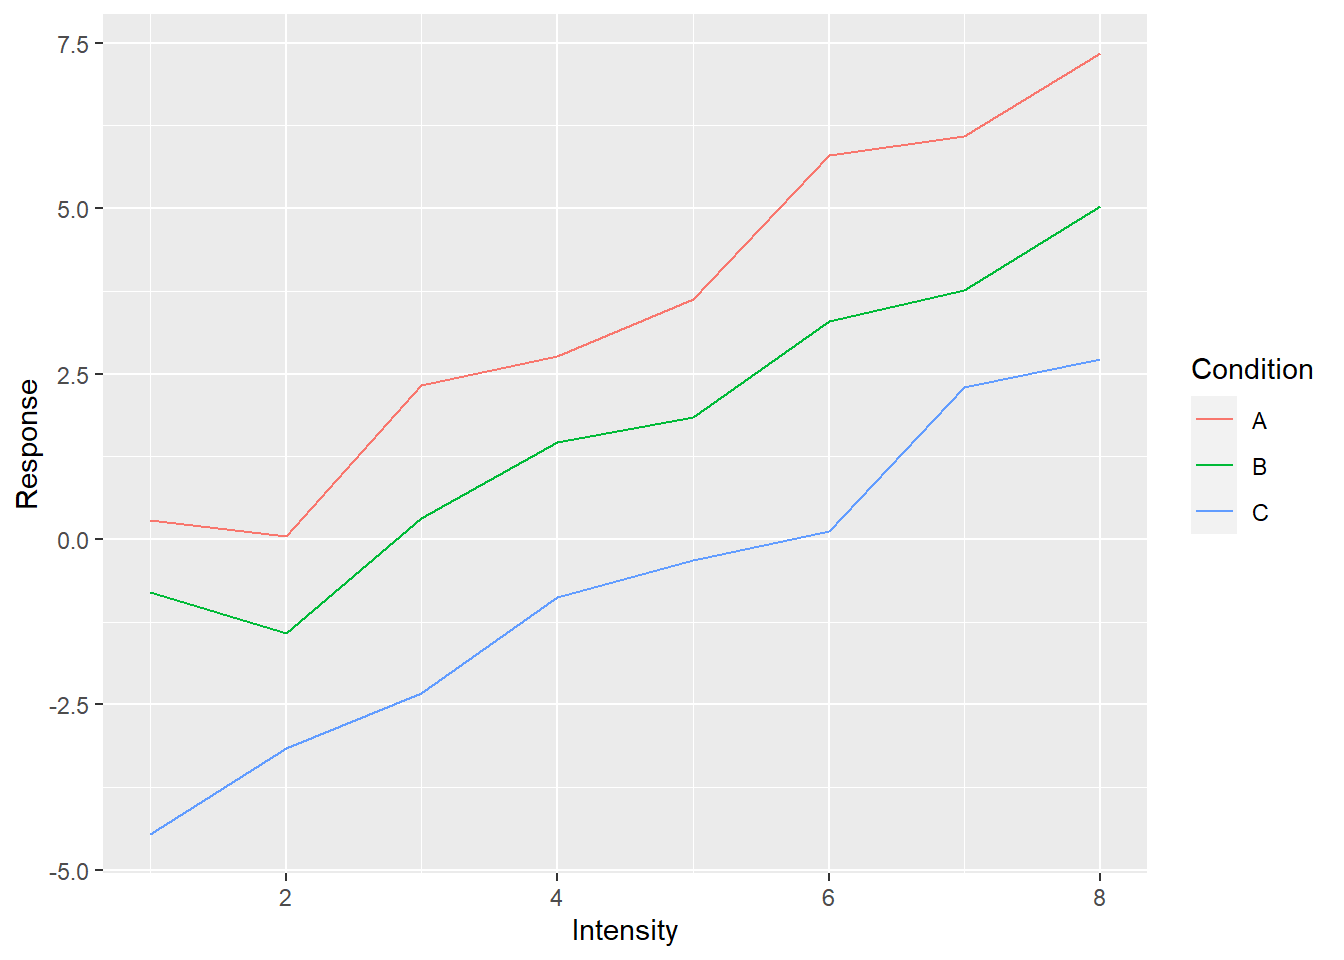
\includegraphics{data-analysis-using-r-for-psychology_files/figure-latex/unnamed-chunk-116-1.pdf}

As I already wrote, technically, the only thing you need to define is aesthetics, so let us not add anything to the plot (we drop the \texttt{+geom\_line()}).

\begin{Shaded}
\begin{Highlighting}[]
\FunctionTok{ggplot}\NormalTok{(}\AttributeTok{data=}\NormalTok{simple\_tidy\_data, }\FunctionTok{aes}\NormalTok{(}\AttributeTok{x =}\NormalTok{ Intensity, }\AttributeTok{y =}\NormalTok{ Response, }\AttributeTok{color=}\NormalTok{Condition))}
\end{Highlighting}
\end{Shaded}

\begin{center}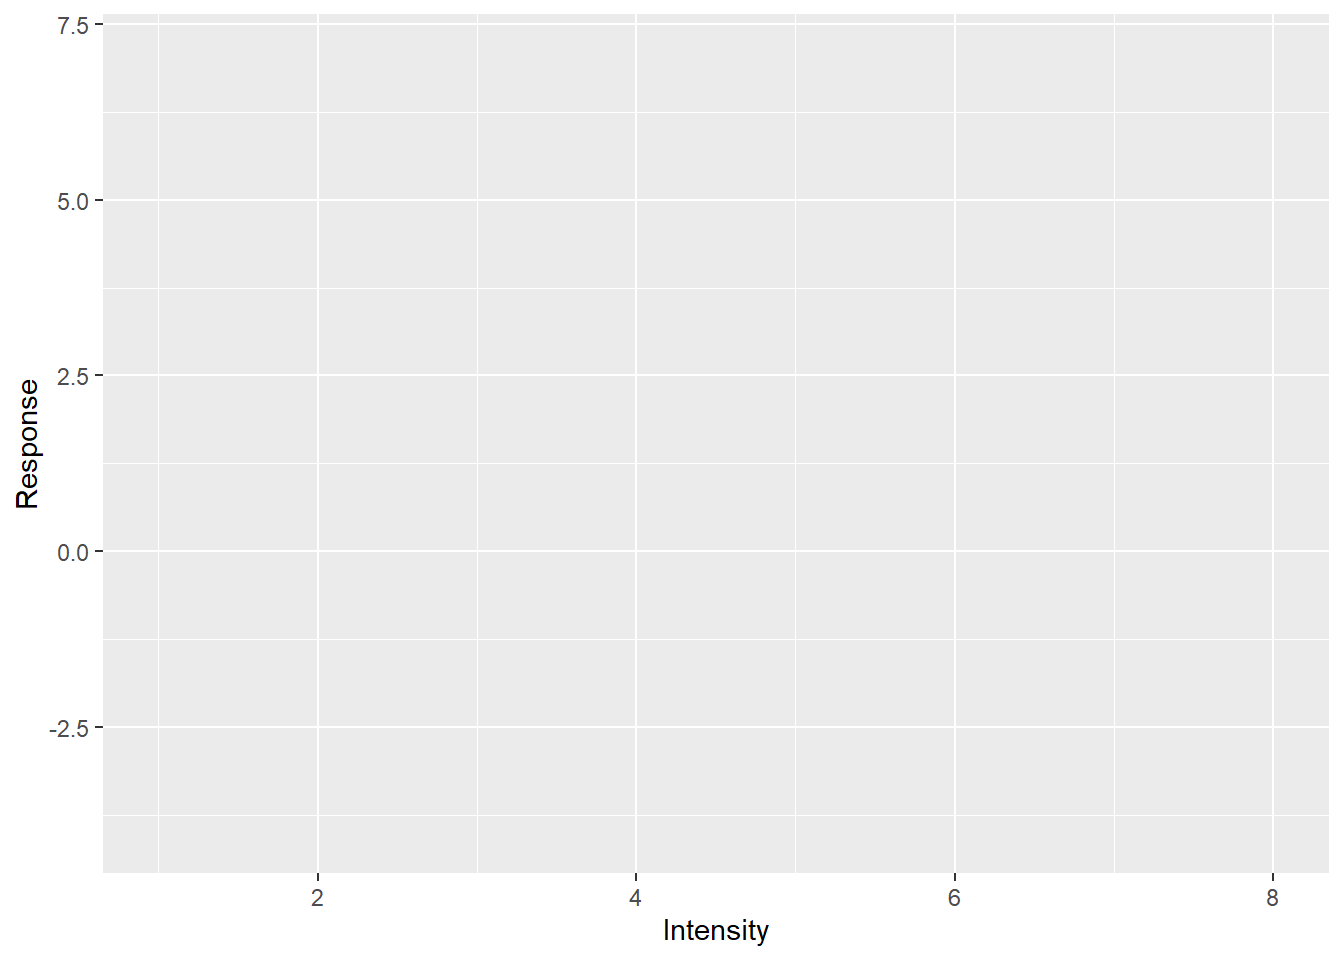
\includegraphics{data-analysis-using-r-for-psychology_files/figure-latex/unnamed-chunk-117-1} \end{center}

Told you it will look empty and yet you can already see \emph{ggplot2} in action. Notice that axes are labeled and their limits are set. You cannot see the legend (they are not plotted without corresponding geometry) but it is also ready behind the scenes. This is because our initial call specified the most important part: how individual variables map on various properties even before we tell \emph{ggplot2} which visuals we will use to plot the data. When we specified that x-axis will represent the \texttt{Intensity}, ggplot2 figured out the range of values, so it knows \emph{where} it is going to plot whatever we decide to plot. Points, lines, bars, error bars and what not will span only that range. Same goes for other properties such as color. We wanted \emph{color} to represent the condition. Again, we may not know what exactly we will be plotting (points, lines?) or even how many different visuals we will be adding to the plot (just lines? points + lines? points + lines + linear fit?) but we do know that whatever visual we add, if it can have color, its color \emph{must} represent condition for that data point. The beauty of \emph{ggplot2} is that it analyses your data and figures out how many colors you need and is ready to apply them \emph{consistently} to all visuals you will add later. It will ensure that all points, bars, lines, etc. will have consistent coordinates scaling, color, size, fill mapping that are the same across the entire plot. This may sound trivial but typically (e.g., Matlab, Matplotlib), it is \emph{your} job to make sure that all these properties match and that they represent the same value across all visual elements. And this is a pretty tedious job, particularly when you decide to change your mappings and have to redo all individual components by hand. In \emph{ggplot2}, this dissociation between mapping and visuals means you can tinker with one of them at a time. E.g. keep the visuals but change grouping or see if effect of condition is easier to see via line type, size or shape of the point? Or you can keep the mapping and see whether adding another visual will make the plot easier to understand. Note that some mapping also \emph{groups} your data, so when you use group-based visual information (e.g., a linear regression line) it will know what data belongs together and so will perform this computation per group.

Let us see how you can keep the relationship mapping but add more visuals. Let us add both lines and points.

\begin{Shaded}
\begin{Highlighting}[]
\FunctionTok{ggplot}\NormalTok{(}\AttributeTok{data=}\NormalTok{simple\_tidy\_data, }\FunctionTok{aes}\NormalTok{(}\AttributeTok{x =}\NormalTok{ Intensity, }\AttributeTok{y =}\NormalTok{ Response, }\AttributeTok{color=}\NormalTok{Condition)) }\SpecialCharTok{+} 
  \FunctionTok{geom\_line}\NormalTok{() }\SpecialCharTok{+}
  \FunctionTok{geom\_point}\NormalTok{() }\CommentTok{\# this is new!}
\end{Highlighting}
\end{Shaded}

\begin{center}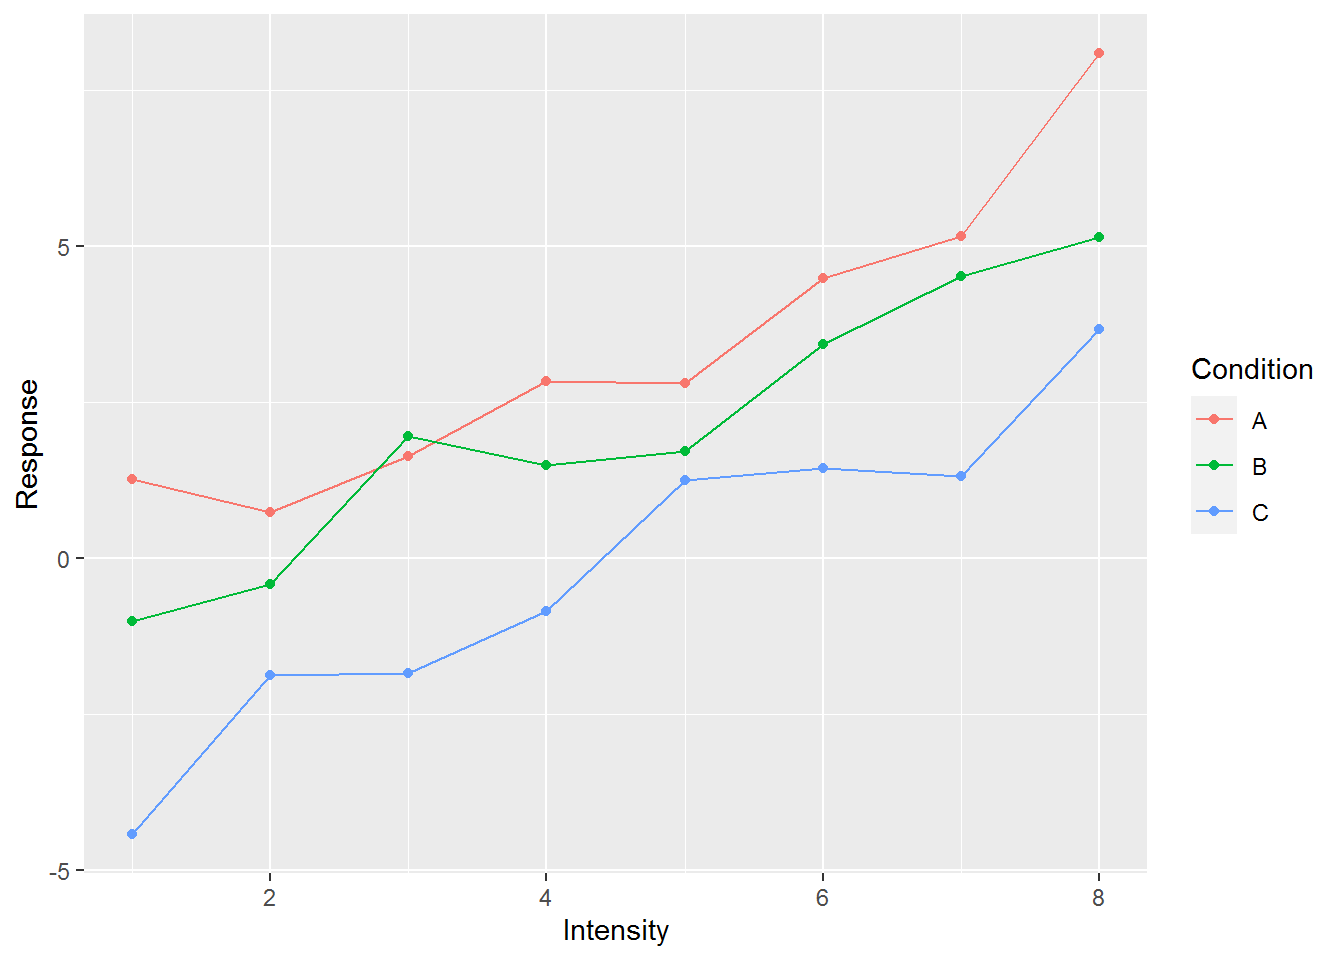
\includegraphics{data-analysis-using-r-for-psychology_files/figure-latex/unnamed-chunk-118-1} \end{center}

In the plot above, we \emph{kept} the relationship between variables and properties but said ``Oh, and throw in some points please''. And ggplot2 knows how to add the points so that they appear at proper location and in proper color. But we want more!

\begin{Shaded}
\begin{Highlighting}[]
\FunctionTok{ggplot}\NormalTok{(}\AttributeTok{data=}\NormalTok{simple\_tidy\_data, }\FunctionTok{aes}\NormalTok{(}\AttributeTok{x =}\NormalTok{ Intensity, }\AttributeTok{y =}\NormalTok{ Response, }\AttributeTok{color=}\NormalTok{Condition)) }\SpecialCharTok{+} 
  \FunctionTok{geom\_line}\NormalTok{() }\SpecialCharTok{+}
  \FunctionTok{geom\_point}\NormalTok{() }\SpecialCharTok{+}
  \CommentTok{\# a linear regression over all dots in the group}
  \FunctionTok{geom\_smooth}\NormalTok{(}\AttributeTok{method=}\StringTok{"lm"}\NormalTok{, }\AttributeTok{formula =}\NormalTok{ y }\SpecialCharTok{\textasciitilde{}}\NormalTok{ x, }\AttributeTok{se=}\ConstantTok{FALSE}\NormalTok{, }\AttributeTok{linetype=}\StringTok{"dashed"}\NormalTok{) }
\end{Highlighting}
\end{Shaded}

\begin{center}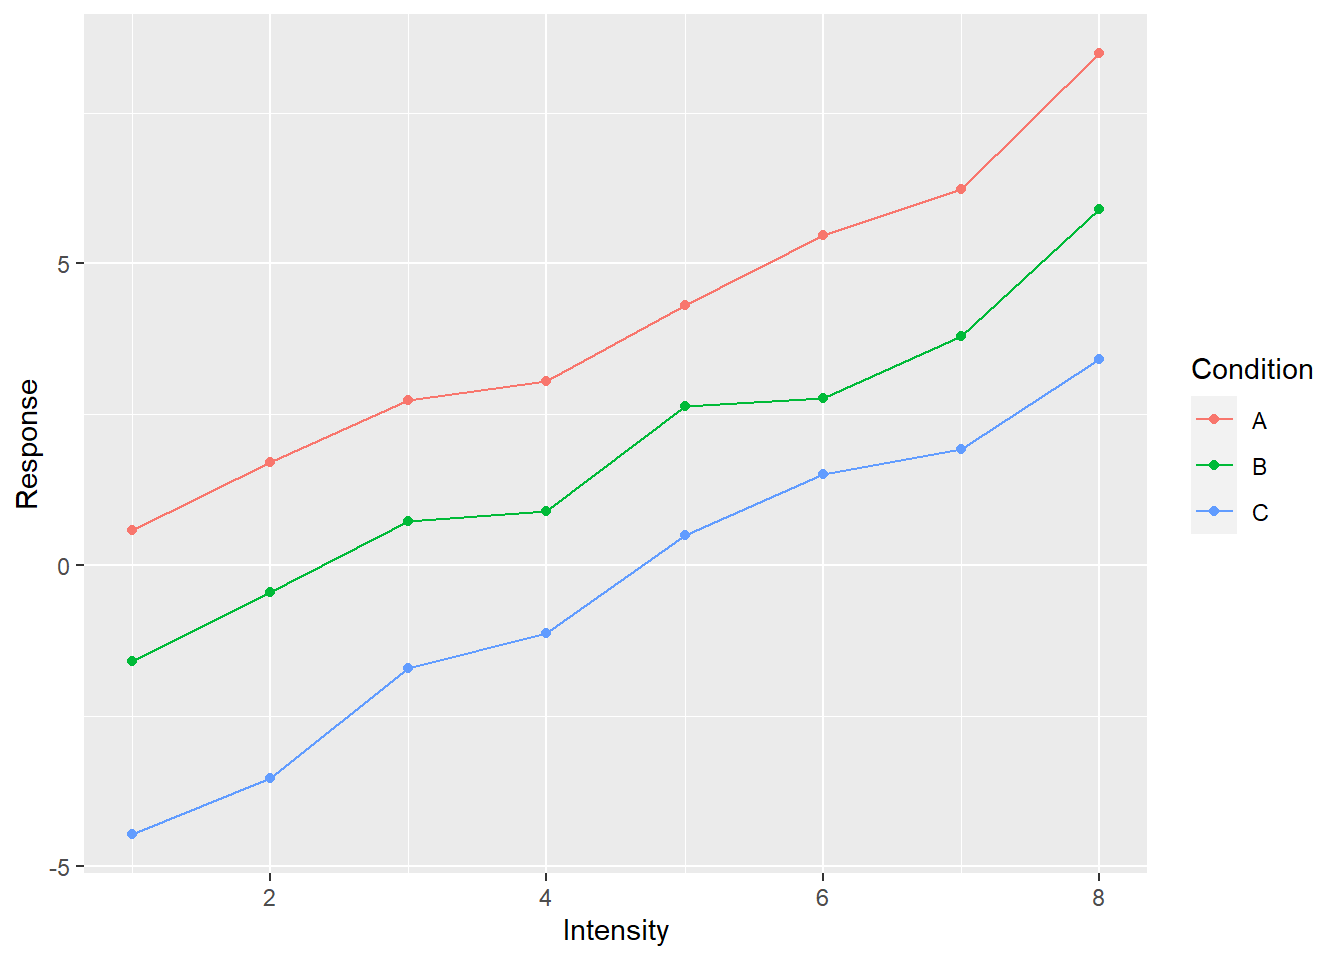
\includegraphics{data-analysis-using-r-for-psychology_files/figure-latex/unnamed-chunk-119-1} \end{center}

Now we added a linear regression line that helps us to better see the relationship between \texttt{Intensity} and \texttt{Response}. Again, we simply wished for another visual to be added (\texttt{method="lm"} means that we wanted to average data via linear regression with \texttt{formula\ =\ y\ \textasciitilde{}\ x} meaning that we regress y-axis on x-axis with no further covariates, \texttt{se=FALSE} means no standard error stripe, \texttt{linetype="dashed"} just makes it easier to distinguish linar fit from the solid data line).

Or, we can keep the \emph{visuals} but see whether changing \emph{mapping} would make it more informative (we need to specify \texttt{group=Intensity} as continuous data is not grouped automatically).

\begin{Shaded}
\begin{Highlighting}[]
\FunctionTok{ggplot}\NormalTok{(}\AttributeTok{data=}\NormalTok{simple\_tidy\_data, }\FunctionTok{aes}\NormalTok{(}\AttributeTok{x =}\NormalTok{ Condition, }\AttributeTok{y =}\NormalTok{ Response, }\AttributeTok{color=}\NormalTok{Intensity, }\AttributeTok{group=}\NormalTok{Intensity)) }\SpecialCharTok{+} 
  \FunctionTok{geom\_line}\NormalTok{() }\SpecialCharTok{+}
  \FunctionTok{geom\_point}\NormalTok{() }\SpecialCharTok{+}
  \FunctionTok{geom\_smooth}\NormalTok{(}\AttributeTok{method=}\StringTok{"lm"}\NormalTok{, }\AttributeTok{se=}\ConstantTok{FALSE}\NormalTok{,  }\AttributeTok{formula =}\NormalTok{ y }\SpecialCharTok{\textasciitilde{}}\NormalTok{ x, }\AttributeTok{linetype=}\StringTok{"dashed"}\NormalTok{)}
\end{Highlighting}
\end{Shaded}

\begin{center}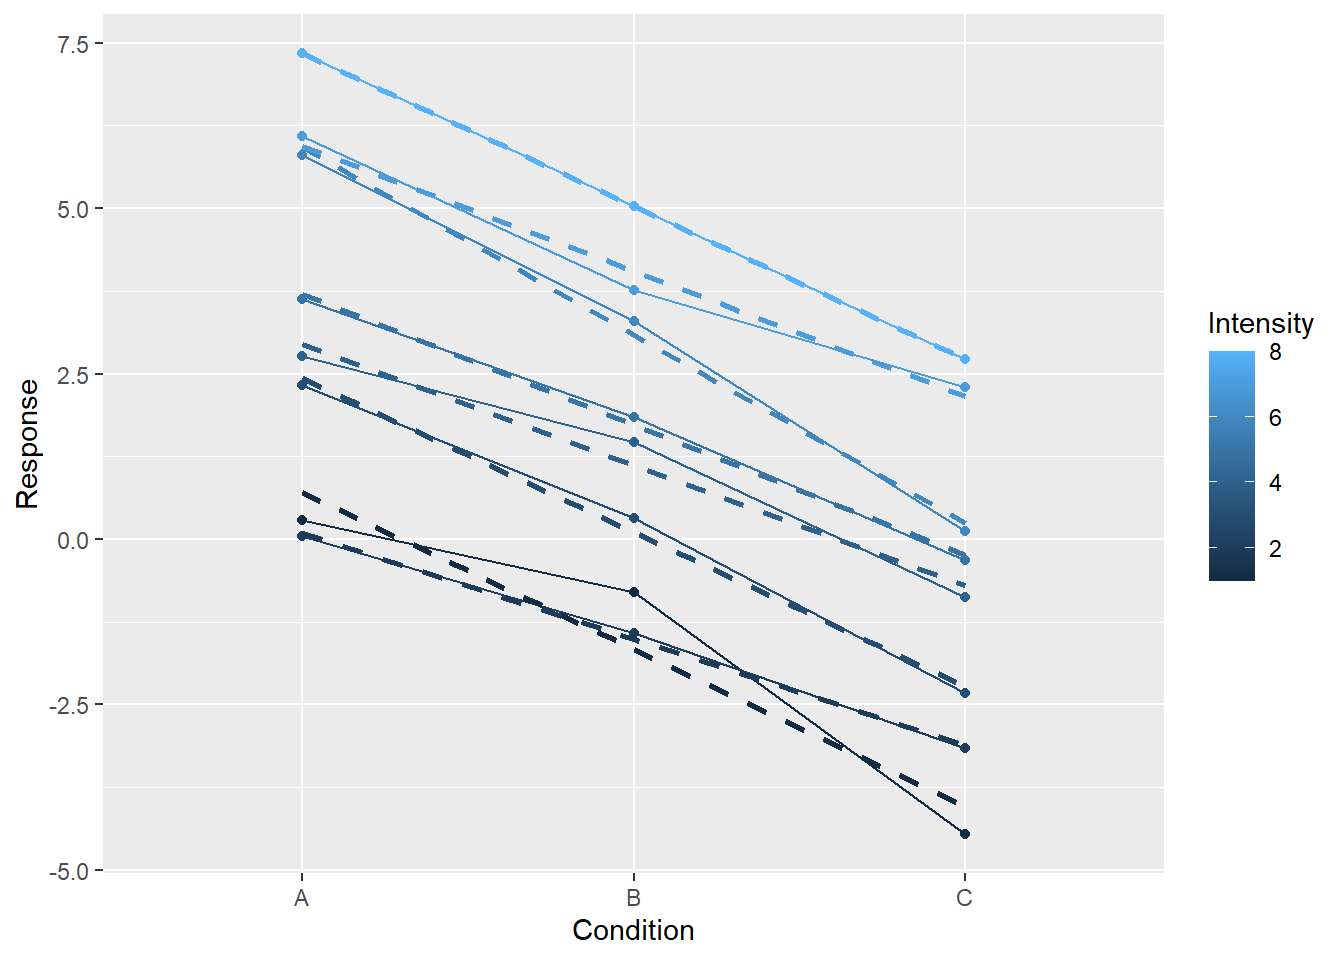
\includegraphics{data-analysis-using-r-for-psychology_files/figure-latex/unnamed-chunk-120-1} \end{center}

Or, we can check whether splitting into several plots helps.

\begin{Shaded}
\begin{Highlighting}[]
\FunctionTok{ggplot}\NormalTok{(}\AttributeTok{data=}\NormalTok{simple\_tidy\_data, }\FunctionTok{aes}\NormalTok{(}\AttributeTok{x =}\NormalTok{ Intensity, }\AttributeTok{y =}\NormalTok{ Response, }\AttributeTok{color=}\NormalTok{Condition)) }\SpecialCharTok{+} 
  \FunctionTok{geom\_line}\NormalTok{() }\SpecialCharTok{+}
  \FunctionTok{geom\_point}\NormalTok{() }\SpecialCharTok{+}
  \FunctionTok{geom\_smooth}\NormalTok{(}\AttributeTok{method=}\StringTok{"lm"}\NormalTok{, }\AttributeTok{formula =}\NormalTok{ y }\SpecialCharTok{\textasciitilde{}}\NormalTok{ x, }\AttributeTok{se=}\ConstantTok{FALSE}\NormalTok{, }\AttributeTok{linetype=}\StringTok{"dashed"}\NormalTok{) }\SpecialCharTok{+}
  \FunctionTok{facet\_grid}\NormalTok{(. }\SpecialCharTok{\textasciitilde{}}\NormalTok{ Condition) }\CommentTok{\# makes a separate subplot for each group}
\end{Highlighting}
\end{Shaded}

\begin{center}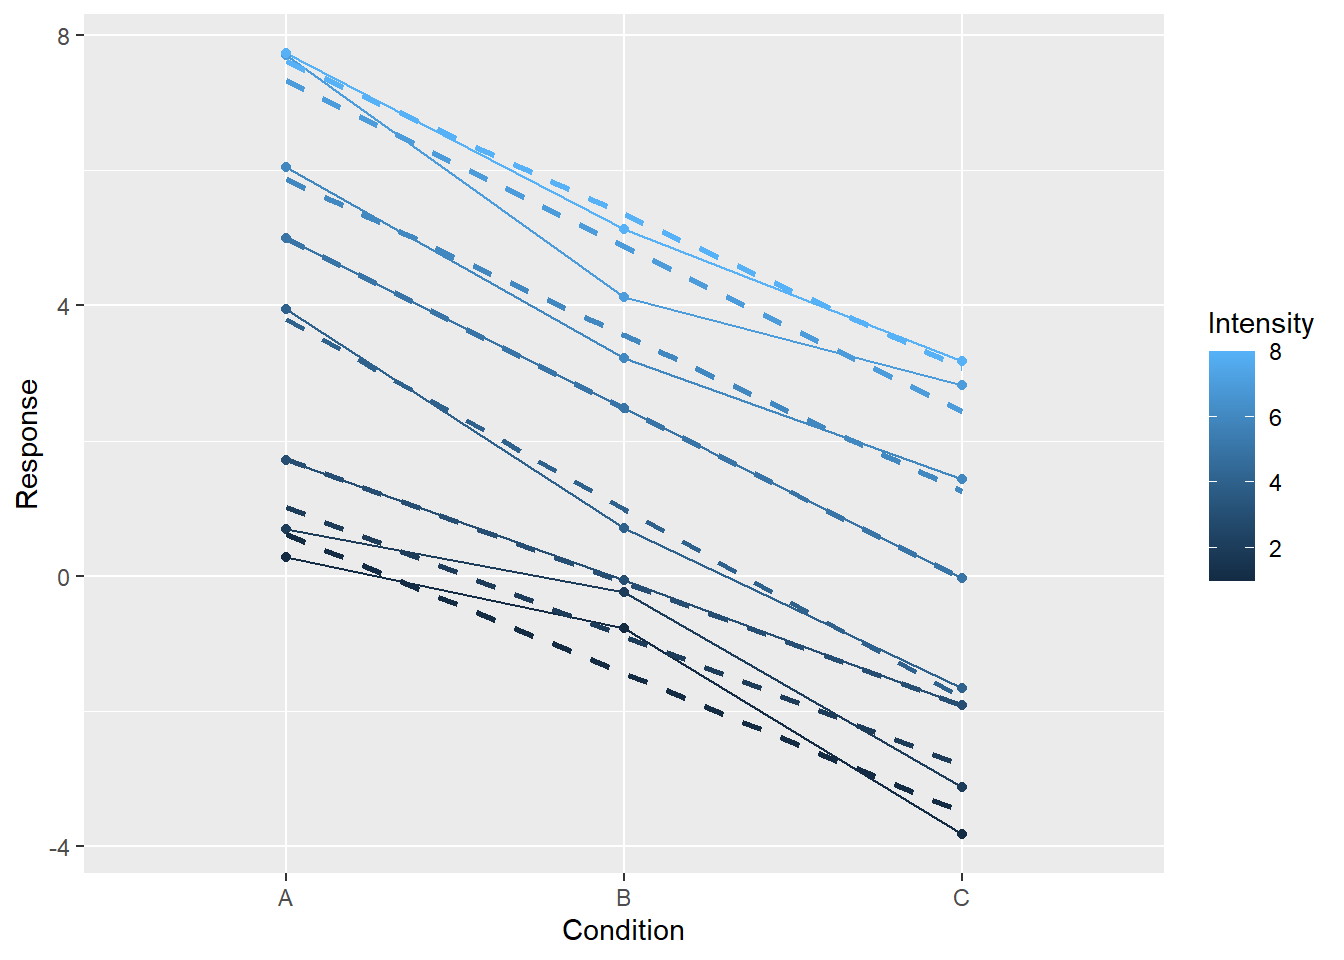
\includegraphics{data-analysis-using-r-for-psychology_files/figure-latex/unnamed-chunk-121-1} \end{center}

Again, note that all three plots live on the same scale for x- and y-axis, making them easy to compare (you fully appreciate this magic if you ever struggled with ensuring optimal and consistent scaling by hand in Matlab). I went through so many examples to stress how ggplot allows you to think about the aesthetics of variable mapping \emph{independently} of the actual visual representation (and vice versa).

Now lets us explore \emph{ggplot2} by doing exercises. I recommend using \href{https://ggplot2.tidyverse.org/}{ggplot2 reference page} and \href{https://github.com/rstudio/cheatsheets/raw/master/data-visualization-2.1.pdf}{cheatsheet} when you are doing the exercises.

\hypertarget{auto-efficiency-continuous-x-axis}{%
\section{Auto efficiency: continuous x-axis}\label{auto-efficiency-continuous-x-axis}}

We start by visualizing how car efficiency, measured as miles-per-gallon, is affected by various factors such as production year, size of the engine, type of transmission, etc. The data is in the table \href{https://ggplot2.tidyverse.org/reference/mpg.html}{mpg}, which is part of the \emph{ggplot2} package. Thus, you need to first \protect\hyperlink{library}{import} the library and then load the table via \protect\hyperlink{data}{data()} function. Take a look at the \href{https://ggplot2.tidyverse.org/reference/mpg.html}{table description} to familiarize yourself with the variables.

First, let us look at the relationship between car efficiency in the city cycle (\texttt{cty}), engine displacement (\texttt{displ}), and drive train type (\texttt{drv}) using color points. Reminder, the call should look as

\begin{verbatim}
ggplot(data_table_name, [aes](https://ggplot2.tidyverse.org/reference/aes.html)(x = var1, y = var2, color = var3, shape = var4, ...)) + 
  geom_primitive1() + 
  geom_primitive2() +
  ...
\end{verbatim}

Think about which variables are mapped on each axes and which is best depicted as color.

Do exercise 1.

Do you see any clear dependence? Let us try to making it more evident by adding \href{https://ggplot2.tidyverse.org/reference/geom_smooth.html}{geom\_smooth} geometric primitive.

Do exercise 2.

Both engine size (displacement) and drive train have a clear effect on car efficiency. Let us visualize the number of cylinders (\texttt{cyl}) as well. Including it by mapping it on the \emph{size} of geometry.

Do exercise 3.

Currently, we are mixing together cars produced at different times. Let us visually separate them by turning each year into a subplot via \href{https://ggplot2.tidyverse.org/reference/facet_wrap.html}{facet\_wrap} function.

Do exercise 4.

The dependence you plotted does not look linear but instead is saturating at certain low level of efficiency. This sort of dependencies could be easier to see on a logarithmic scale. See functions for different \href{https://ggplot2.tidyverse.org/reference/scale_continuous.html}{scales} and use logarithmic scaling for y-axis.

Do exercise 5.

Note that by now we managed to include \emph{five} variables into our plots. We can continue this by including transmission or fuel type but that would be pushing it, as too many variables can make a plot confusing and cryptic. Instead, let us make it prettier by using more meaningful axes labels (\texttt{xlab()}, \texttt{ylab()} functions) and adding a plot title (\href{https://ggplot2.tidyverse.org/reference/labs.html}{labs}).

Do exercise 6.

\hypertarget{auto-efficiency-discrete-x-axis}{%
\section{Auto efficiency: discrete x-axis}\label{auto-efficiency-discrete-x-axis}}

The previous section use a continuous engine displacement variable for x-axis (at least that is my assumption on how you mapped the variables). Frequently, you need to plot data for discrete groups: experimental groups, conditions, treatments, etc. Let us practice on the same \href{https://ggplot2.tidyverse.org/reference/mpg.html}{mpg} data set but visualize relationship between the drive train (\texttt{drv}) and highway cycle efficiency (\texttt{hwy}). Start by using point as visuals.

Do exercise 7.

One problem with the plot is that all points are plotted at the same x-axis location. This means that if two points share the location, they overlap and appear as just one dot. This makes it hard to understand the density: one point can mean one point, or two, or a hundred. A better way to plot such data is by using \href{https://ggplot2.tidyverse.org/reference/geom_boxplot.html}{box} or \href{https://ggplot2.tidyverse.org/reference/geom_violin.html}{violin} plots. Experiment by using them instead of points.

Do exercise 8.

Again, let's up the ante and split plots via both number of cylinders and year of manufacturing. Use \href{https://ggplot2.tidyverse.org/reference/facet_grid.html}{facet\_grid} function to generate grid of plots.

Do exercise 9.

Let us again improve our presentation by using better axes labels and figure title.

Do exercise 10.

\hypertarget{mammals-sleep-single-variable}{%
\section{Mammals sleep: single variable}\label{mammals-sleep-single-variable}}

Now lets us work on plotting a distribution for a single variable using \href{https://ggplot2.tidyverse.org/reference/msleep.html}{mammals sleep dataset}. For this, you need to map \texttt{sleep\_total} variable on x-axis and plot a \href{https://ggplot2.tidyverse.org/reference/geom_histogram.html}{histogram}. Explore the available options, in particular \texttt{bins} that determines the bins number and, therefore, their size. Note that there is no ``correct'' number of bins to use. \emph{ggplot2} defaults to 30 but a small sample would be probably better served with fewer bins and, vice versa, with a large data set you can afford hundred of bins.

Do exercise 11.

Using a histogram gives you exact counts per each bin. However, the appearance may change quite dramatically if you would use fewer or more bins. An alternative way to represent the same information is via \href{https://ggplot2.tidyverse.org/reference/geom_density.html}{smoothed density estimates}. They use a sliding window and compute an estimate at each point but also include points \emph{around} it and weight them according to a kernel (e.g., a Gaussian one). This makes the plot look smoother and will mask sudden jumps in density (counts) as you, effectively, average over many bins. Whether this approach is better for visualizing data depends on the sample you have and message you are trying to get across. It is always worth checking both (just like it is worth checking different number of bins in histogram) to see which way is the best for your specific case.

Do exercise 12.

Let us return to using histograms and plot a distribution per \texttt{vore} variable (it is \texttt{carnivore}, \texttt{omnivore}, \texttt{herbivore}, or \texttt{NA}). You can map it on the \texttt{fill} color of the histogram, so that each \emph{vore} kind will be binned separately.

Do exercise 13.

The plot may look confusing because by default \emph{ggplot2} colors values for each group differently but stacks all of them together to produce the total histogram counts. One way to disentangle the individual histograms is via \href{https://ggplot2.tidyverse.org/reference/facet_grid.html}{facet\_grid} function. Use it to plot \texttt{vore} distribution in separate rows.

Do exercise 14.

That did the trick but there is an alternative way to plot individual distributions on the same plot by setting \texttt{position} argument of geom\_histogram to \texttt{"identity"} (it is \texttt{"stack"} by default).

Do exercise 15.

Hmm, shouldn't we have more carnivores, what is going on? Opacity is the answer. A bar ``in front'' occludes any bars that are ``behind'' it. Go back to the exercise and fix that by specifying \texttt{alpha} argument that controls transparency. It is \texttt{1} (completely opaque) by default and can go down to \texttt{0} (fully transparent as in ``invisible''), so see which intermediate value works the best.

\hypertarget{mapping-for-all-visuals-versus-just-one-visual}{%
\section{Mapping for all visuals versus just one visual}\label{mapping-for-all-visuals-versus-just-one-visual}}

In the previous exercise, you assigned a constant value to \texttt{alpha} (transparency) argument. You could do this in \emph{two} places, inside of either \texttt{ggplot()} or \texttt{geom\_histogram()} call. In the former case, you would have set \texttt{alpha} level for \emph{all} geometric primitives on the plot, whereas in the latter you do it only for the histogram. To better see the difference, reuse your code for plotting city cycle efficiency versus engine size (should be exercise \#6) and set \texttt{alpha} either for all visuals (in \texttt{ggplot2}) or in some visuals (e.g.~only for points) to see the difference.

Do exercise 16.

\hypertarget{mapping-on-variables-versus-constants}{%
\section{Mapping on variables versus constants}\label{mapping-on-variables-versus-constants}}

In the previous exercise, you assigned a constant value to \texttt{alpha} (transparency) argument. However, transparency is just a property just like \texttt{x}, \texttt{color}, or \texttt{size}. Thus, there are \emph{two} ways you can use them:

\begin{itemize}
\tightlist
\item
  \emph{inside} \texttt{aes(x=column)}, where \texttt{column} is column in the table you supplied via \texttt{data=}
\item
  \emph{outside} of \texttt{aes} by stating \texttt{x=value}, where value is some constant value or a variable \emph{that is not in the table}.
\end{itemize}

Test this but setting the \texttt{size} in the previous plot to a constant outside of aesthetics or to a variable inside of it.

Do exercise 17.

\hypertarget{themes}{%
\section{Themes}\label{themes}}

Finally, if you are not a fan of the way the plots look, you can quickly modify this by using some other theme. You can define it yourself (there are lots of options you can specify for your \href{https://ggplot2.tidyverse.org/reference/theme.html}{theme}) or can use one of the \href{https://ggplot2.tidyverse.org/reference/ggtheme.html}{ready-mades}. Explore the latter option, find the one you like the best.

Do exercise 18.

\hypertarget{you-aint-seen-nothing-yet}{%
\section{You ain't seen nothing yet}\label{you-aint-seen-nothing-yet}}

What you explored is just a tip of the iceberg. There are many more geometric primitive, annotations, scales, themes, etc. It will take an entire separate seminar to do \emph{ggplot2} justice. However, the basics will get you started and you can always consult reference, books (see below), or me once you need more.

\hypertarget{further-reading}{%
\section{Further reading}\label{further-reading}}

If plotting data is part of your daily routine, I recommend reading \href{https://ggplot2-book.org/}{ggplot2 book}. It gives you an in-depth view of the package and goes through many possibilities that it offers. You may need all of them but I find useful to know that they exists (who knows, I might need them one day). Another book worth reading is \href{https://kieranhealy.org/publications/dataviz/}{Data Visualization: A Practical Introduction.} by Kieran Healy.

\hypertarget{extending-ggplot2}{%
\section{Extending ggplot2}\label{extending-ggplot2}}

There are 102 (as of 21.10.2021) extensions that you find at \href{https://exts.ggplot2.tidyverse.org/gallery/}{ggplot2 website}. They add more ways to plot your data, more themes, animated plots, etc. If you feel that \emph{ggplot2} does not have the geometric primitives you need, take a look at the gallery and, most likely, you will find something that fits your bill.

One package that is \emph{not} in the gallery is \href{https://patchwork.data-imaginist.com/}{patchwork}. It was created ``to make it ridiculously simple to combine separate ggplots into the same graphic''. It is a bold promise but authors do make good on it. It is probably the easiest way to combine multiple plots but you can also consider \href{https://github.com/wilkelab/cowplot}{cowplot} and \href{https://cran.r-project.org/web/packages/gridExtra/index.html}{gridExtra} packages.

\hypertarget{ggplot2-cannot-do-everything}{%
\section{ggplot2 cannot do everything}\label{ggplot2-cannot-do-everything}}

There are many different plotting routines and packages for R but I would recommend to use \emph{ggplot2} as your main tool. However, that does not mean that it must be your only tool, after all, CRAN is brimming with packages. In particular, \emph{ggplot2} is built for plotting data from a single tidy table, meaning it is less optimal for plotting data in other cases. E.g., you can use it to combine information from several tables in one plot but things become less automatic and consistent. Similarly, you can plot data which is stored in non-tidy tables or even in individual vectors but that makes it less intuitive and more convoluted. No package can do everything and \emph{ggplot2} is no exception.

\hypertarget{dplyr}{%
\chapter{Tidyverse: dplyr}\label{dplyr}}

Now that you understand vectors, tables, functions and pipes, and you know what our end goal (a tidy table) is, we can start with data analysis and Tidyverse way of doing it. All functions discussed below are part of \href{https://dplyr.tidyverse.org/}{dplyr}\footnote{The name should invoke an image of data pliers. According to Hadley Wickham, you can pronounce it any way you like.} ``grammar of data manipulation'' package. Grab the \href{notebooks/Seminar\%2006\%20-\%20dplyr.Rmd}{exercise notebook}!

\hypertarget{tidyverse-philosophy}{%
\section{Tidyverse philosophy}\label{tidyverse-philosophy}}

Data analysis is different from ``normal'' programming as it mostly involves a series of sequential operations on the same table. You might load the table, transform some variables, filter data, select smaller subset of columns, aggregate by summarizing across different groups of variables before plotting it or formally analyzing it via statistical tests. Tidyverse is built around this serial nature of data analysis of piping a table through a chain of functions. Accordingly, Tidyverse functions take a \emph{table} (\texttt{data.frame} or \texttt{tibble}) as their \emph{first} parameter, which makes piping simpler, and return a \emph{modified table} as an output. This \emph{table-in → table-out} consistency makes it easy to pipe these operations one after another. For me, it helps to think about Tidyverse functions as \emph{verbs}: Actions that I perform on the table at each step.

Here is quick teaser of how such sequential piping works. Below, we will examine each verb/function separately and I will also show you how same operations can be carried out using base R. Note that I put each verb/function on a separate line. This makes it easier to understand how many different operations you perform (number of lines), how complex they are (how long individuals lines of code are), and makes them easy to read line-by-line.

\begin{Shaded}
\begin{Highlighting}[]
\NormalTok{mpg2lpk }\OtherTok{\textless{}{-}} \FloatTok{2.82481061}

\NormalTok{mpg }\SpecialCharTok{\%\textgreater{}\%}
  \CommentTok{\# we filter the table by rows, }
  \CommentTok{\# only keeping rows for which year is 2008}
  \FunctionTok{filter}\NormalTok{(year }\SpecialCharTok{==} \DecValTok{2008}\NormalTok{) }\SpecialCharTok{\%\textgreater{}\%}
  
  \CommentTok{\# we change cty and hwy columns by turning}
  \CommentTok{\# miles/gallon into liters/kilometer}
  \FunctionTok{mutate}\NormalTok{(}\AttributeTok{cty =}\NormalTok{ cty }\SpecialCharTok{/}\NormalTok{ mpg2lpk,}
         \AttributeTok{hwy =}\NormalTok{ hwy }\SpecialCharTok{/}\NormalTok{ mpg2lpk) }\SpecialCharTok{\%\textgreater{}\%}
  
  \CommentTok{\# we create a new column by computing an }
  \CommentTok{\# average efficiency as mean between city and highway cycles}
  \FunctionTok{mutate}\NormalTok{(}\AttributeTok{avg\_mpg =}\NormalTok{ (cty }\SpecialCharTok{+}\NormalTok{ hwy) }\SpecialCharTok{/} \DecValTok{2}\NormalTok{) }\SpecialCharTok{\%\textgreater{}\%}
  
  \CommentTok{\# we reduce the table to only two columns}
  \CommentTok{\# class (of car) and avg\_mpg}
  \FunctionTok{select}\NormalTok{(class, avg\_mpg) }\SpecialCharTok{\%\textgreater{}\%}
  
  \CommentTok{\# we group by each class of car}
  \CommentTok{\# and compute average efficiency for each group (class of car)}
  \FunctionTok{group\_by}\NormalTok{(class) }\SpecialCharTok{\%\textgreater{}\%}
  \FunctionTok{summarise}\NormalTok{(}\AttributeTok{class\_avg\_mpg =} \FunctionTok{mean}\NormalTok{(avg\_mpg), }\AttributeTok{.groups=}\StringTok{"keep"}\NormalTok{) }\SpecialCharTok{\%\textgreater{}\%}
  
  \CommentTok{\# we sort table rows to go from worst to best on efficiency}
  \FunctionTok{arrange}\NormalTok{(class\_avg\_mpg) }\SpecialCharTok{\%\textgreater{}\%}
  
  \CommentTok{\# we kable (Knit the tABLE) to make it look nicer in the document}
\NormalTok{  knitr}\SpecialCharTok{::}\FunctionTok{kable}\NormalTok{()}
\end{Highlighting}
\end{Shaded}

\begin{tabular}{l|r}
\hline
class & class\_avg\_mpg\\
\hline
pickup & 5.299679\\
\hline
suv & 5.707006\\
\hline
minivan & 6.655313\\
\hline
2seater & 7.139122\\
\hline
subcompact & 8.153201\\
\hline
midsize & 8.386572\\
\hline
compact & 8.721421\\
\hline
\end{tabular}

\hypertarget{select}{%
\section{\texorpdfstring{\texttt{select()} columns by name}{select() columns by name}}\label{select}}

\href{https://dplyr.tidyverse.org/reference/select.html}{Select} verb allows you to select/pick columns in a table using their names. This is very similar to using columns names as indexes for tables that you have learned in \protect\hyperlink{table-indexing}{seminar 3}.

First, let us make a shorter version of \texttt{mpg} table by keeping only the first five rows. Note that you can also pick first N rows via \href{https://stat.ethz.ch/R-manual/R-devel/library/utils/html/head.html}{head()} function.

\begin{Shaded}
\begin{Highlighting}[]
\NormalTok{short\_mpg }\OtherTok{\textless{}{-}}\NormalTok{ mpg[}\DecValTok{1}\SpecialCharTok{:}\DecValTok{5}\NormalTok{, ]}

\CommentTok{\# same "first five rows" but via head() function}
\NormalTok{short\_mpg }\OtherTok{\textless{}{-}} \FunctionTok{head}\NormalTok{(mpg, }\DecValTok{5}\NormalTok{)}

\NormalTok{knitr}\SpecialCharTok{::}\FunctionTok{kable}\NormalTok{(short\_mpg)}
\end{Highlighting}
\end{Shaded}

\begin{tabular}{l|l|r|r|r|l|l|r|r|l|l}
\hline
manufacturer & model & displ & year & cyl & trans & drv & cty & hwy & fl & class\\
\hline
audi & a4 & 1.8 & 1999 & 4 & auto(l5) & f & 18 & 29 & p & compact\\
\hline
audi & a4 & 1.8 & 1999 & 4 & manual(m5) & f & 21 & 29 & p & compact\\
\hline
audi & a4 & 2.0 & 2008 & 4 & manual(m6) & f & 20 & 31 & p & compact\\
\hline
audi & a4 & 2.0 & 2008 & 4 & auto(av) & f & 21 & 30 & p & compact\\
\hline
audi & a4 & 2.8 & 1999 & 6 & auto(l5) & f & 16 & 26 & p & compact\\
\hline
\end{tabular}

Here is how you can select only \texttt{model} and \texttt{cty} columns via preserving \texttt{{[}{]}} subsetting

\begin{Shaded}
\begin{Highlighting}[]
\NormalTok{short\_mpg[, }\FunctionTok{c}\NormalTok{(}\StringTok{"model"}\NormalTok{, }\StringTok{"cty"}\NormalTok{)] }
\end{Highlighting}
\end{Shaded}

\begin{tabular}{l|r}
\hline
model & cty\\
\hline
a4 & 18\\
\hline
a4 & 21\\
\hline
a4 & 20\\
\hline
a4 & 21\\
\hline
a4 & 16\\
\hline
\end{tabular}

And here is how it is done via \texttt{select()}.

\begin{Shaded}
\begin{Highlighting}[]
\NormalTok{short\_mpg }\SpecialCharTok{\%\textgreater{}\%}
  \FunctionTok{select}\NormalTok{(model, cty)}
\end{Highlighting}
\end{Shaded}

\begin{tabular}{l|r}
\hline
model & cty\\
\hline
a4 & 18\\
\hline
a4 & 21\\
\hline
a4 & 20\\
\hline
a4 & 21\\
\hline
a4 & 16\\
\hline
\end{tabular}

The idea of Tidyverse functions is to adopt to you, so you \emph{can} use quotes or pass a vector of strings with column names. All calls below produce the same effect, so pick the style you prefer (mine, is in the code \emph{above}) and stick to it\footnote{In general, bad but consistent styling is better than an inconsistent mix of good styles.}.

\begin{Shaded}
\begin{Highlighting}[]
\NormalTok{short\_mpg }\SpecialCharTok{\%\textgreater{}\%}
  \FunctionTok{select}\NormalTok{(}\FunctionTok{c}\NormalTok{(}\StringTok{"model"}\NormalTok{, }\StringTok{"cty"}\NormalTok{))}
  
\NormalTok{short\_mpg }\SpecialCharTok{\%\textgreater{}\%}
  \FunctionTok{select}\NormalTok{(}\StringTok{"model"}\NormalTok{, }\StringTok{"cty"}\NormalTok{)}
  
\NormalTok{short\_mpg }\SpecialCharTok{\%\textgreater{}\%}
  \FunctionTok{select}\NormalTok{(}\FunctionTok{c}\NormalTok{(model, cty))}
\end{Highlighting}
\end{Shaded}

As you surely remember, you can use negation to select \emph{other} indexes within a vector (\texttt{c(4,\ 5,\ 6){[}-2{]}} gives you \texttt{{[}4,\ 6{]}}). For the single brackets \texttt{{[}{]}} this mechanism does not work with column \emph{names} (only with their indexes). However, \texttt{select} has you covered, so we can select everything \emph{but} \texttt{cty} and \texttt{model}

\begin{Shaded}
\begin{Highlighting}[]
\NormalTok{short\_mpg }\SpecialCharTok{\%\textgreater{}\%}
  \FunctionTok{select}\NormalTok{(}\SpecialCharTok{{-}}\NormalTok{cty, }\SpecialCharTok{{-}}\NormalTok{model)}
\end{Highlighting}
\end{Shaded}

\begin{tabular}{l|r|r|r|l|l|r|l|l}
\hline
manufacturer & displ & year & cyl & trans & drv & hwy & fl & class\\
\hline
audi & 1.8 & 1999 & 4 & auto(l5) & f & 29 & p & compact\\
\hline
audi & 1.8 & 1999 & 4 & manual(m5) & f & 29 & p & compact\\
\hline
audi & 2.0 & 2008 & 4 & manual(m6) & f & 31 & p & compact\\
\hline
audi & 2.0 & 2008 & 4 & auto(av) & f & 30 & p & compact\\
\hline
audi & 2.8 & 1999 & 6 & auto(l5) & f & 26 & p & compact\\
\hline
\end{tabular}

In the current version of \texttt{dplyr}, you can do the same negation via \texttt{!} (a \texttt{logical\ not} operator, you will meet later), moreover, it is now a recommended way of writing the selection\footnote{At least, \texttt{-} is not mentioned anymore, even though it still works.}. The \texttt{-} and \texttt{!} are not synonyms and the difference is subtle but important, see below.

\begin{Shaded}
\begin{Highlighting}[]
\CommentTok{\# will produce the same result as above}
\NormalTok{short\_mpg }\SpecialCharTok{\%\textgreater{}\%}
  \FunctionTok{select}\NormalTok{(}\SpecialCharTok{!}\NormalTok{cty, }\SpecialCharTok{!}\NormalTok{model)}
\end{Highlighting}
\end{Shaded}

As with the direct selection above, you can use negation with names as strings, you can negate a vector of names, etc. Again, it is mostly a matter of taste with consistency being more important than a specific choice you make.

\begin{Shaded}
\begin{Highlighting}[]
\CommentTok{\# will produce the same result as above}
\NormalTok{short\_mpg }\SpecialCharTok{\%\textgreater{}\%}
  \FunctionTok{select}\NormalTok{(}\SpecialCharTok{!}\FunctionTok{c}\NormalTok{(}\StringTok{"cty"}\NormalTok{, }\StringTok{"model"}\NormalTok{))}

\NormalTok{short\_mpg }\SpecialCharTok{\%\textgreater{}\%}
  \FunctionTok{select}\NormalTok{(}\SpecialCharTok{!}\StringTok{"cty"}\NormalTok{, }\SpecialCharTok{!}\StringTok{"model"}\NormalTok{)}
  
\NormalTok{short\_mpg }\SpecialCharTok{\%\textgreater{}\%}
  \FunctionTok{select}\NormalTok{(}\SpecialCharTok{!}\FunctionTok{c}\NormalTok{(cty, model))}
\end{Highlighting}
\end{Shaded}

Unlike vector indexing that forbids mixing positive and negative indexing, \texttt{select} does allow it. However, \textbf{do not use it}\footnote{Unless you know what you are doing and that is the simplest and clearest way to achieve this.} because results can be fairly counter-intuitive and, on top of that, \texttt{-} and \texttt{!} work somewhat differently. Note the difference between \texttt{!} and \texttt{-}: In the former case only the \texttt{!model} part appears to have the effect, whereas in case of \texttt{-} only \texttt{cty} works.

\begin{Shaded}
\begin{Highlighting}[]
\NormalTok{short\_mpg }\SpecialCharTok{\%\textgreater{}\%}
  \FunctionTok{select}\NormalTok{(cty, }\SpecialCharTok{!}\NormalTok{model)}
\end{Highlighting}
\end{Shaded}

\begin{tabular}{r|l|r|r|r|l|l|r|l|l}
\hline
cty & manufacturer & displ & year & cyl & trans & drv & hwy & fl & class\\
\hline
18 & audi & 1.8 & 1999 & 4 & auto(l5) & f & 29 & p & compact\\
\hline
21 & audi & 1.8 & 1999 & 4 & manual(m5) & f & 29 & p & compact\\
\hline
20 & audi & 2.0 & 2008 & 4 & manual(m6) & f & 31 & p & compact\\
\hline
21 & audi & 2.0 & 2008 & 4 & auto(av) & f & 30 & p & compact\\
\hline
16 & audi & 2.8 & 1999 & 6 & auto(l5) & f & 26 & p & compact\\
\hline
\end{tabular}

\begin{Shaded}
\begin{Highlighting}[]
\NormalTok{short\_mpg }\SpecialCharTok{\%\textgreater{}\%}
  \FunctionTok{select}\NormalTok{(cty, }\SpecialCharTok{{-}}\NormalTok{model)}
\end{Highlighting}
\end{Shaded}

\begin{tabular}{r}
\hline
cty\\
\hline
18\\
\hline
21\\
\hline
20\\
\hline
21\\
\hline
16\\
\hline
\end{tabular}

To make things even, worse \texttt{select(-model,\ cty)} work the same way as \texttt{select(cty,\ !model)} (sigh\ldots)

\begin{Shaded}
\begin{Highlighting}[]
\NormalTok{short\_mpg }\SpecialCharTok{\%\textgreater{}\%}
  \FunctionTok{select}\NormalTok{(}\SpecialCharTok{{-}}\NormalTok{model, cty)}
\end{Highlighting}
\end{Shaded}

\begin{tabular}{l|r|r|r|l|l|r|r|l|l}
\hline
manufacturer & displ & year & cyl & trans & drv & cty & hwy & fl & class\\
\hline
audi & 1.8 & 1999 & 4 & auto(l5) & f & 18 & 29 & p & compact\\
\hline
audi & 1.8 & 1999 & 4 & manual(m5) & f & 21 & 29 & p & compact\\
\hline
audi & 2.0 & 2008 & 4 & manual(m6) & f & 20 & 31 & p & compact\\
\hline
audi & 2.0 & 2008 & 4 & auto(av) & f & 21 & 30 & p & compact\\
\hline
audi & 2.8 & 1999 & 6 & auto(l5) & f & 16 & 26 & p & compact\\
\hline
\end{tabular}

So, bottom line, do not mix positive and negative indexing in \texttt{select}! I am showing you this only to signal the potential danger.

Do exercise 1.

Simple names and their negation will be sufficient for most of your projects. However, I would recommend taking a look at the \href{https://dplyr.tidyverse.org/reference/select.html}{official manual} just to see that \texttt{select} offers a lot of flexibility (selecting range of columns, by column type, by partial name matching, etc), something that might be useful for you in your work.

\hypertarget{conditions}{%
\section{Conditions}\label{conditions}}

Before we can work with the next verb, you need to understand conditions. Conditions are statements about values that are either \texttt{TRUE} or \texttt{FALSE}. In the simplest case, you can check whether two values (one in a variable and one hard-coded) are equal via \texttt{==} operator

\begin{Shaded}
\begin{Highlighting}[]
\NormalTok{x }\OtherTok{\textless{}{-}} \DecValTok{5}
\FunctionTok{print}\NormalTok{(x }\SpecialCharTok{==} \DecValTok{5}\NormalTok{)}
\end{Highlighting}
\end{Shaded}

\begin{verbatim}
## [1] TRUE
\end{verbatim}

\begin{Shaded}
\begin{Highlighting}[]
\FunctionTok{print}\NormalTok{(x }\SpecialCharTok{==} \DecValTok{3}\NormalTok{)}
\end{Highlighting}
\end{Shaded}

\begin{verbatim}
## [1] FALSE
\end{verbatim}

For numeric values, you can use all usual comparison operators including \emph{not equal} \texttt{!=}, \emph{less than} \texttt{\textless{}}, \emph{greater than} \texttt{\textgreater{}}, \emph{less than or equal to} \texttt{\textless{}=} (note the order of symbols!), and \emph{greater than or equal to} \texttt{\textgreater{}=} (again, note the order of symbols).

Do exercise 2.

You can negate a statement via \emph{not} \texttt{!} symbol as \texttt{!TRUE} is \texttt{FALSE} and vice versa. However, note that round brackets in the examples below! They are critical to express the \emph{order} of computation. Anything \emph{inside} the brackets is evaluated first. And if you have brackets inside the brackets, similar to nested functions, it is the innermost expression that get evaluated first. In the example below, \texttt{x==5} is evaluated first and logical inversion happens only after it. In this particular example, you may not need them but I would suggest using them to ensure clarity.

\begin{Shaded}
\begin{Highlighting}[]
\NormalTok{x }\OtherTok{\textless{}{-}} \DecValTok{5}
\FunctionTok{print}\NormalTok{(}\SpecialCharTok{!}\NormalTok{(x }\SpecialCharTok{==} \DecValTok{5}\NormalTok{))}
\end{Highlighting}
\end{Shaded}

\begin{verbatim}
## [1] FALSE
\end{verbatim}

\begin{Shaded}
\begin{Highlighting}[]
\FunctionTok{print}\NormalTok{(}\SpecialCharTok{!}\NormalTok{(x }\SpecialCharTok{==} \DecValTok{3}\NormalTok{))}
\end{Highlighting}
\end{Shaded}

\begin{verbatim}
## [1] TRUE
\end{verbatim}

Do exercise 3.

You can also combine several conditions using \emph{and} \texttt{\&} and \emph{or} \texttt{\textbar{}} operators. Again, note round brackets that explicitly define what is evaluated first.

\begin{Shaded}
\begin{Highlighting}[]
\NormalTok{x }\OtherTok{\textless{}{-}} \DecValTok{5}
\NormalTok{y }\OtherTok{\textless{}{-}} \DecValTok{2}

\CommentTok{\# x is not equal to 5 OR y is equal to 1}
\FunctionTok{print}\NormalTok{((x }\SpecialCharTok{!=} \DecValTok{5}\NormalTok{) }\SpecialCharTok{|}\NormalTok{ (y }\SpecialCharTok{==} \DecValTok{1}\NormalTok{))}
\end{Highlighting}
\end{Shaded}

\begin{verbatim}
## [1] FALSE
\end{verbatim}

\begin{Shaded}
\begin{Highlighting}[]
\CommentTok{\# x less than 10 AND y is greater than or equal to 1}
\FunctionTok{print}\NormalTok{((x }\SpecialCharTok{\textless{}} \DecValTok{10}\NormalTok{) }\SpecialCharTok{\&}\NormalTok{ (y }\SpecialCharTok{\textgreater{}=} \DecValTok{1}\NormalTok{))}
\end{Highlighting}
\end{Shaded}

\begin{verbatim}
## [1] TRUE
\end{verbatim}

Do exercise 4.

All examples above used scalars but you remember that \emph{everything is a vector}, including values that we used (they are just vectors of length one). Accordingly, same logic works for vectors of arbitrary length with comparisons working element-wise, so you get a vector of the same length with \texttt{TRUE} or \texttt{FALSE} values for each \emph{pairwise} comparison.

Do exercise 5.

\hypertarget{logical-indexing}{%
\section{Logical indexing}\label{logical-indexing}}

In the second seminar, you learned about vector indexing when you access \emph{some} elements of a vector by specifying their index. There is an alternative way, called \emph{logical indexing}. Here, you supply a vector of equal length with \emph{logical values} and you get elements of the original vector whenever the logical value is \texttt{TRUE}

\begin{Shaded}
\begin{Highlighting}[]
\NormalTok{x }\OtherTok{\textless{}{-}} \DecValTok{1}\SpecialCharTok{:}\DecValTok{5}
\NormalTok{x[}\FunctionTok{c}\NormalTok{(}\ConstantTok{TRUE}\NormalTok{, }\ConstantTok{TRUE}\NormalTok{, }\ConstantTok{FALSE}\NormalTok{, }\ConstantTok{TRUE}\NormalTok{, }\ConstantTok{FALSE}\NormalTok{)]}
\end{Highlighting}
\end{Shaded}

\begin{verbatim}
## [1] 1 2 4
\end{verbatim}

This is particularly useful, if you are interested in elements that satisfy certain condition. For example, you want all \emph{negative} values and you can use condition \texttt{x\textless{}5} that will produce a vector of logical values that, in turn, can be used as index

\begin{Shaded}
\begin{Highlighting}[]
\NormalTok{x }\OtherTok{\textless{}{-}} \FunctionTok{c}\NormalTok{(}\SpecialCharTok{{-}}\DecValTok{2}\NormalTok{, }\DecValTok{5}\NormalTok{, }\DecValTok{3}\NormalTok{, }\SpecialCharTok{{-}}\DecValTok{5}\NormalTok{, }\SpecialCharTok{{-}}\DecValTok{1}\NormalTok{)}
\NormalTok{x[x}\SpecialCharTok{\textless{}}\DecValTok{0}\NormalTok{]}
\end{Highlighting}
\end{Shaded}

\begin{verbatim}
## [1] -2 -5 -1
\end{verbatim}

You can have conditions of any complexity by combining them via \emph{and} \texttt{\&} and \emph{or} \texttt{\textbar{}} operators. For example, if you want number below -1 or above 3 (be careful to have space between \texttt{\textless{}} and \texttt{-}, otherwise it will be interpreted as assignment \texttt{\textless{}-}).

\begin{Shaded}
\begin{Highlighting}[]
\NormalTok{x }\OtherTok{\textless{}{-}} \FunctionTok{c}\NormalTok{(}\SpecialCharTok{{-}}\DecValTok{2}\NormalTok{, }\DecValTok{5}\NormalTok{, }\DecValTok{3}\NormalTok{, }\SpecialCharTok{{-}}\DecValTok{5}\NormalTok{, }\SpecialCharTok{{-}}\DecValTok{1}\NormalTok{)}
\NormalTok{x[(x}\SpecialCharTok{\textless{}} \SpecialCharTok{{-}}\DecValTok{1}\NormalTok{) }\SpecialCharTok{|}\NormalTok{ (x}\SpecialCharTok{\textgreater{}}\DecValTok{3}\NormalTok{)]}
\end{Highlighting}
\end{Shaded}

\begin{verbatim}
## [1] -2  5 -5
\end{verbatim}

Do exercise 6.

Sometimes you may want to know the actual index of elements for \emph{which} some condition is \texttt{TRUE}. Function \href{https://stat.ethz.ch/R-manual/R-devel/library/base/html/which.html}{which()} does exactly that.

\begin{Shaded}
\begin{Highlighting}[]
\NormalTok{x }\OtherTok{\textless{}{-}} \FunctionTok{c}\NormalTok{(}\SpecialCharTok{{-}}\DecValTok{2}\NormalTok{, }\DecValTok{5}\NormalTok{, }\DecValTok{3}\NormalTok{, }\SpecialCharTok{{-}}\DecValTok{5}\NormalTok{, }\SpecialCharTok{{-}}\DecValTok{1}\NormalTok{)}
\FunctionTok{which}\NormalTok{( (x}\SpecialCharTok{\textless{}} \SpecialCharTok{{-}}\DecValTok{1}\NormalTok{) }\SpecialCharTok{|}\NormalTok{ (x}\SpecialCharTok{\textgreater{}}\DecValTok{3}\NormalTok{) )}
\end{Highlighting}
\end{Shaded}

\begin{verbatim}
## [1] 1 2 4
\end{verbatim}

\hypertarget{filter-rows-by-values}{%
\section{\texorpdfstring{\texttt{filter()} rows by values}{filter() rows by values}}\label{filter-rows-by-values}}

Now that you understand conditions and logical indexing, using \href{https://dplyr.tidyverse.org/reference/filter.html}{filter()} is very straightforward: You simply put condition that describes rows that you want to \emph{retain} inside the \texttt{filter()} call. For example, we can look at efficiency only for two-seater cars.

\begin{Shaded}
\begin{Highlighting}[]
\NormalTok{mpg }\SpecialCharTok{\%\textgreater{}\%}
  \FunctionTok{filter}\NormalTok{(class }\SpecialCharTok{==} \StringTok{"2seater"}\NormalTok{)}
\end{Highlighting}
\end{Shaded}

\begin{tabular}{l|l|r|r|r|l|l|r|r|l|l}
\hline
manufacturer & model & displ & year & cyl & trans & drv & cty & hwy & fl & class\\
\hline
chevrolet & corvette & 5.7 & 1999 & 8 & manual(m6) & r & 16 & 26 & p & 2seater\\
\hline
chevrolet & corvette & 5.7 & 1999 & 8 & auto(l4) & r & 15 & 23 & p & 2seater\\
\hline
chevrolet & corvette & 6.2 & 2008 & 8 & manual(m6) & r & 16 & 26 & p & 2seater\\
\hline
chevrolet & corvette & 6.2 & 2008 & 8 & auto(s6) & r & 15 & 25 & p & 2seater\\
\hline
chevrolet & corvette & 7.0 & 2008 & 8 & manual(m6) & r & 15 & 24 & p & 2seater\\
\hline
\end{tabular}

You can use information from any row, so we can look for midsize cars with four-wheel drive.

\begin{Shaded}
\begin{Highlighting}[]
\NormalTok{mpg }\SpecialCharTok{\%\textgreater{}\%}
  \FunctionTok{filter}\NormalTok{(class }\SpecialCharTok{==} \StringTok{"midsize"} \SpecialCharTok{\&}\NormalTok{ drv }\SpecialCharTok{==} \StringTok{"4"}\NormalTok{)}
\end{Highlighting}
\end{Shaded}

\begin{tabular}{l|l|r|r|r|l|l|r|r|l|l}
\hline
manufacturer & model & displ & year & cyl & trans & drv & cty & hwy & fl & class\\
\hline
audi & a6 quattro & 2.8 & 1999 & 6 & auto(l5) & 4 & 15 & 24 & p & midsize\\
\hline
audi & a6 quattro & 3.1 & 2008 & 6 & auto(s6) & 4 & 17 & 25 & p & midsize\\
\hline
audi & a6 quattro & 4.2 & 2008 & 8 & auto(s6) & 4 & 16 & 23 & p & midsize\\
\hline
\end{tabular}

Do exercise 7.

Note that you can emulate \texttt{filter()} in a very straightforward way using single-brackets base R, the main difference is that you need to prefix every column with the table name, so \texttt{mpg{[}{[}"class"{]}{]}} instead of just \texttt{class}\footnote{You can sidestep this issue via \href{https://stat.ethz.ch/R-manual/R-devel/library/base/html/with.html}{with()} function, although I am not a big fan of this approach.}.

\begin{Shaded}
\begin{Highlighting}[]
\NormalTok{mpg[mpg[[}\StringTok{"class"}\NormalTok{]] }\SpecialCharTok{==} \StringTok{"midsize"} \SpecialCharTok{\&}\NormalTok{ mpg[[}\StringTok{"drv"}\NormalTok{]] }\SpecialCharTok{==} \StringTok{"4"}\NormalTok{, ]}
\end{Highlighting}
\end{Shaded}

\begin{tabular}{l|l|r|r|r|l|l|r|r|l|l}
\hline
manufacturer & model & displ & year & cyl & trans & drv & cty & hwy & fl & class\\
\hline
audi & a6 quattro & 2.8 & 1999 & 6 & auto(l5) & 4 & 15 & 24 & p & midsize\\
\hline
audi & a6 quattro & 3.1 & 2008 & 6 & auto(s6) & 4 & 17 & 25 & p & midsize\\
\hline
audi & a6 quattro & 4.2 & 2008 & 8 & auto(s6) & 4 & 16 & 23 & p & midsize\\
\hline
\end{tabular}

So why use \texttt{filter()} then? In isolation, as a single line computation, both options are equally compact and clear (apart from all the extra \texttt{table{[}{[}"..."{]}{]}} in base R). But pipe-oriented nature of the \texttt{filter()} makes it more suitable for chains of computations, which is the main advantage of Tidyverse.

\hypertarget{arrange-rows-in-a-particular-order}{%
\section{\texorpdfstring{\texttt{arrange()} rows in a particular order}{arrange() rows in a particular order}}\label{arrange-rows-in-a-particular-order}}

Sometimes you might need to sort your table so that rows go in a particular order\footnote{In my experience, this mostly happens when you need to print out or view a table.}. In Tidyverse, you \href{https://dplyr.tidyverse.org/reference/arrange.html}{arrange} rows based on values of specific variables. This verb is very straightforward, you simply list all variables that must be used for sorting in the order the sorting must be carried out. I.e., first the table is sorted based on values of the first variable. Then, for equal values of that variable, rows are sorted based on the second variable, etc. By default, rows are arranged in ascending order but you can reverse it by putting a variable inside of \href{https://dplyr.tidyverse.org/reference/desc.html}{desc()} function. Here is the \texttt{short\_mpg} table arranged by city cycle highway efficiency (ascending order) and engine displacement (descending order, note the order of the last two rows).

\begin{Shaded}
\begin{Highlighting}[]
\NormalTok{short\_mpg }\SpecialCharTok{\%\textgreater{}\%}
  \FunctionTok{arrange}\NormalTok{(cty, }\FunctionTok{desc}\NormalTok{(displ)) }
\end{Highlighting}
\end{Shaded}

\begin{tabular}{l|l|r|r|r|l|l|r|r|l|l}
\hline
manufacturer & model & displ & year & cyl & trans & drv & cty & hwy & fl & class\\
\hline
audi & a4 & 2.8 & 1999 & 6 & auto(l5) & f & 16 & 26 & p & compact\\
\hline
audi & a4 & 1.8 & 1999 & 4 & auto(l5) & f & 18 & 29 & p & compact\\
\hline
audi & a4 & 2.0 & 2008 & 4 & manual(m6) & f & 20 & 31 & p & compact\\
\hline
audi & a4 & 2.0 & 2008 & 4 & auto(av) & f & 21 & 30 & p & compact\\
\hline
audi & a4 & 1.8 & 1999 & 4 & manual(m5) & f & 21 & 29 & p & compact\\
\hline
\end{tabular}

Do exercise 8.

You can arrange a table using base R via \href{https://stat.ethz.ch/R-manual/R-devel/library/base/html/order.html}{order()} function that gives index of ordered elements and can be used inside of preserving subsetting via single brackets \texttt{{[}{]}} notation. You can control for ascending/descending of a specific variable using \href{https://stat.ethz.ch/R-manual/R-devel/library/base/html/rev.html}{rev()} function that is applied \emph{after} ordering, so \texttt{rev(order(...))}.

\begin{Shaded}
\begin{Highlighting}[]
\NormalTok{short\_mpg[}\FunctionTok{order}\NormalTok{(short\_mpg[[}\StringTok{"cty"}\NormalTok{]], }\FunctionTok{rev}\NormalTok{(short\_mpg[[}\StringTok{"displ"}\NormalTok{]])), ]}
\end{Highlighting}
\end{Shaded}

\begin{tabular}{l|l|r|r|r|l|l|r|r|l|l}
\hline
manufacturer & model & displ & year & cyl & trans & drv & cty & hwy & fl & class\\
\hline
audi & a4 & 2.8 & 1999 & 6 & auto(l5) & f & 16 & 26 & p & compact\\
\hline
audi & a4 & 1.8 & 1999 & 4 & auto(l5) & f & 18 & 29 & p & compact\\
\hline
audi & a4 & 2.0 & 2008 & 4 & manual(m6) & f & 20 & 31 & p & compact\\
\hline
audi & a4 & 2.0 & 2008 & 4 & auto(av) & f & 21 & 30 & p & compact\\
\hline
audi & a4 & 1.8 & 1999 & 4 & manual(m5) & f & 21 & 29 & p & compact\\
\hline
\end{tabular}

Do exercise 9.

\hypertarget{mutate}{%
\section{\texorpdfstring{\texttt{mutate()} columns}{mutate() columns}}\label{mutate}}

In Tidyverse, \href{https://dplyr.tidyverse.org/reference/mutate.html}{mutate} function allows you to both add new columns/variables to a table and change the existing ones. In essence, it is equivalent to a simple column assignment statement in base R.

\begin{Shaded}
\begin{Highlighting}[]
\CommentTok{\# base R}
\NormalTok{short\_mpg[[}\StringTok{"avg\_mpg"}\NormalTok{]] }\OtherTok{\textless{}{-}}\NormalTok{ (short\_mpg[[}\StringTok{"cty"}\NormalTok{]] }\SpecialCharTok{+}\NormalTok{ short\_mpg[[}\StringTok{"hwy"}\NormalTok{]]) }\SpecialCharTok{/} \DecValTok{2}

\CommentTok{\# Tidyverse equivalent}
\NormalTok{short\_mpg }\OtherTok{\textless{}{-}} 
\NormalTok{  short\_mpg }\SpecialCharTok{\%\textgreater{}\%}
  \FunctionTok{mutate}\NormalTok{(}\AttributeTok{avg\_mpg =}\NormalTok{ (cty }\SpecialCharTok{+}\NormalTok{ hwy) }\SpecialCharTok{/} \DecValTok{2}\NormalTok{)}
\end{Highlighting}
\end{Shaded}

Note two critical differences. First, \texttt{mutate()} takes a table as an input and returns a table as an output. This is why you start with a table, pipe it to mutate, and assign the results \emph{back} to the original variable. If you have more verbs/lines, it is the output of the \emph{last} computation that is assigned to the variable on the left-hand side of assignment\footnote{R does have \texttt{-\textgreater{}} statement, so, technically, you can pipe your computation and then assign it to a variable \texttt{table\ \%\textgreater{}\%\ mutate()\ -\textgreater{}\ table}. However, this style is generally discouraged as starting with \texttt{table\ \textless{}-\ table\ \%\textgreater{}\%} makes it clear that you modify and store the computation, whereas \texttt{table\ \%\textgreater{}\%} signals that you pipe the results to an output: console, printed-out table, plot, etc.}. Look at the listing below that indexes each line by when it is executed.

\begin{Shaded}
\begin{Highlighting}[]
\NormalTok{some\_table }\OtherTok{\textless{}{-}}    \CommentTok{\# 3. We assign the result to the original table, only once all the code below has been executed.}
\NormalTok{  some\_table }\SpecialCharTok{\%\textgreater{}\%} \CommentTok{\# 1. We start here, with the original table and pipe to the next computation}
  \FunctionTok{mutate}\NormalTok{(...)    }\CommentTok{\# 2. We add/change columns inside of the table. The output is a table which we use for assignment all the way at the top.}
\end{Highlighting}
\end{Shaded}

Second, you are performing a computation \emph{inside} the call of the \texttt{mutate()} function, so \texttt{avg\_mpg\ =\ (short\_mpg\$cty\ +\ short\_mpg\$hwy)\ /\ 2} is a \emph{parameter} that you pass to it (yes, it does not look like one). This is why you use \texttt{=} rather than a normal assignment arrow \texttt{\textless{}-}. Unfortunately, you \emph{can} use \texttt{\textless{}-} inside the \texttt{mutate} and the computation will work as intended but, for internal-processing reasons, the \emph{entire statement}, rather than just the left-hand side, will be used as a column name. Thus, use \texttt{\textless{}-} \emph{outside} and \texttt{=} \emph{inside} of Tydiverse verbs.

\begin{Shaded}
\begin{Highlighting}[]
\NormalTok{short\_mpg }\SpecialCharTok{\%\textgreater{}\%}
  \FunctionTok{select}\NormalTok{(cty, hwy) }\SpecialCharTok{\%\textgreater{}\%}
  \FunctionTok{mutate}\NormalTok{(}\AttributeTok{avg\_mpg =}\NormalTok{  (cty }\SpecialCharTok{+}\NormalTok{ hwy) }\SpecialCharTok{/} \DecValTok{2}\NormalTok{,      }\CommentTok{\# column name will be avp\_mpg}
\NormalTok{         avg\_mpg }\OtherTok{\textless{}{-}}\NormalTok{ (cty }\SpecialCharTok{+}\NormalTok{ hwy) }\SpecialCharTok{/} \DecValTok{2}\NormalTok{) }\SpecialCharTok{\%\textgreater{}\%} \CommentTok{\# column name will be \textasciigrave{}avg\_mpg \textless{}{-} (short\_mpg$cty + short\_mpg$hwy) / 2\textasciigrave{}}
\NormalTok{  knitr}\SpecialCharTok{::}\FunctionTok{kable}\NormalTok{()}
\end{Highlighting}
\end{Shaded}

\begin{tabular}{r|r|r|r}
\hline
cty & hwy & avg\_mpg & avg\_mpg <- (cty + hwy)/2\\
\hline
18 & 29 & 23.5 & 23.5\\
\hline
21 & 29 & 25.0 & 25.0\\
\hline
20 & 31 & 25.5 & 25.5\\
\hline
21 & 30 & 25.5 & 25.5\\
\hline
16 & 26 & 21.0 & 21.0\\
\hline
\end{tabular}

As shown in the example above, you can perform several computations within a single \texttt{mutate} call and they are executed one after another, just as they would be when using base R.

Do exercise 10.

Finally, \texttt{mutate} has two cousin-verbs called \href{}{transmute} and \href{https://tibble.tidyverse.org/reference/add_column.html}{add\_column}. The former (\texttt{transmute}) works the same way but \emph{discards} all original columns that were not modified. You probably won't use this verb all too often but I want you to be able to recognize it, as its name and function are very similar to \texttt{mutate} and the two are easy to confuse.

\begin{Shaded}
\begin{Highlighting}[]
\NormalTok{short\_mpg }\SpecialCharTok{\%\textgreater{}\%}
  \FunctionTok{transmute}\NormalTok{(}\AttributeTok{avg\_mpg =}\NormalTok{ (cty }\SpecialCharTok{+}\NormalTok{ hwy) }\SpecialCharTok{/} \DecValTok{2}\NormalTok{) }\SpecialCharTok{\%\textgreater{}\%}
\NormalTok{  knitr}\SpecialCharTok{::}\FunctionTok{kable}\NormalTok{(}\AttributeTok{align =} \StringTok{"c"}\NormalTok{)}
\end{Highlighting}
\end{Shaded}

\begin{tabular}{c}
\hline
avg\_mpg\\
\hline
23.5\\
\hline
25.0\\
\hline
25.5\\
\hline
25.5\\
\hline
21.0\\
\hline
\end{tabular}

The latter --- \texttt{add\_column} --- is \emph{similar} to \texttt{mutate} if you need to add a new column rather than to modify a new one. Its advantage is that it will produce an error, if you try to overwrite an existing column. Its disadvantage is that it does not appear to respect data grouping (see below), which can be very confusing. In short, stick to \texttt{mutate} unless you need either of these two functions specifically.

\hypertarget{summarize}{%
\section{\texorpdfstring{\texttt{summarize()} table by \texttt{groups}}{summarize() table by groups}}\label{summarize}}

This verb is used when you \emph{aggregate} across \emph{all} rows, reducing them to a \emph{single value}. Some examples of aggregating functions that are probably already familiar to you are \href{https://stat.ethz.ch/R-manual/R-devel/library/base/html/mean.html}{mean}, \href{https://stat.ethz.ch/R-manual/R-devel/library/stats/html/median.html}{median}, \href{https://stat.ethz.ch/R-manual/R-devel/library/stats/html/sd.html}{standard deviation}, \href{https://stat.ethz.ch/R-manual/R-patched/library/base/html/Extremes.html}{min/max}. However, you can ``aggregate'' by taking a first or a last value or even by putting in a constant. Important is that you should assign a \emph{single} value to the column when using \texttt{summarize}\footnote{In the old times, summarize would only accept a single value and raise an error in any other case. That was good, as it made role of \texttt{summarize} very clear (aggregation) and it was clearly different from \texttt{mutate} (modification). Unfortunately, at certain point of time \texttt{summarize} got a power up, so now it will accept \emph{any} number of values per table/group. This means that, technically, you can use it instead of \texttt{mutate} with no loss of functionality. It also means that it won't warn you that you are doing something wrong in your aggregation, if you return more than one value per group/column. Happened to me often enough to make me wonder why this unfortunate decision was made.}.

If you use \texttt{summarize} on an \emph{ungrouped} table (these are the only tables we've been working on so far), it keeps only the computed columns, which makes you wonder ``what's the point?''

\begin{Shaded}
\begin{Highlighting}[]
\NormalTok{mpg }\SpecialCharTok{\%\textgreater{}\%}
  \FunctionTok{summarise}\NormalTok{(}\AttributeTok{avg\_cty =} \FunctionTok{mean}\NormalTok{(cty),}
            \AttributeTok{avg\_hwy =} \FunctionTok{mean}\NormalTok{(hwy))}
\end{Highlighting}
\end{Shaded}

\begin{verbatim}
## # A tibble: 1 x 2
##   avg_cty avg_hwy
##     <dbl>   <dbl>
## 1    16.9    23.4
\end{verbatim}

However, the real power of \texttt{summarize} (and of \texttt{mutate}) becomes evident when it is applied to the data that is \emph{grouped by} certain criteria. \href{https://dplyr.tidyverse.org/reference/group_by.html}{group\_by()} verb groups rows of the table based on values of variables you specified. Behind the scenes, this turns your single table into set of tables, so that your Tidyverse verbs are applied to \emph{each} table \emph{separately}. This ability to parse your table into different groups of rows (all rows that belong to a particular participant, or participant and condition, or rows per block, or per trial), change that grouping on the fly, return back to the original full table, etc. makes analysis a breeze. Here is how we can compute average efficiency not across all cars (as in the code above) but for each car class separately.

\begin{Shaded}
\begin{Highlighting}[]
\NormalTok{mpg }\SpecialCharTok{\%\textgreater{}\%}
  \CommentTok{\# there are seven different classes of cars, so group\_by(cars)  will}
  \CommentTok{\# create seven hidden independent tables and all verbs below will be }
  \CommentTok{\# applied to each table separately}
  \FunctionTok{group\_by}\NormalTok{(class)  }\SpecialCharTok{\%\textgreater{}\%}
  
  \CommentTok{\# same mean computation but per table and we\textquotesingle{}ve got seven of them}
  \FunctionTok{summarise}\NormalTok{(}\AttributeTok{avg\_cty =} \FunctionTok{mean}\NormalTok{(cty),}
            \AttributeTok{avg\_hwy =} \FunctionTok{mean}\NormalTok{(hwy),}
            \AttributeTok{.groups =} \StringTok{"keep"}\NormalTok{) }\SpecialCharTok{\%\textgreater{}\%}
\NormalTok{  knitr}\SpecialCharTok{::}\FunctionTok{kable}\NormalTok{()}
\end{Highlighting}
\end{Shaded}

\begin{tabular}{l|r|r}
\hline
class & avg\_cty & avg\_hwy\\
\hline
2seater & 15.40000 & 24.80000\\
\hline
compact & 20.12766 & 28.29787\\
\hline
midsize & 18.75610 & 27.29268\\
\hline
minivan & 15.81818 & 22.36364\\
\hline
pickup & 13.00000 & 16.87879\\
\hline
subcompact & 20.37143 & 28.14286\\
\hline
suv & 13.50000 & 18.12903\\
\hline
\end{tabular}

Note that we compute a \emph{single} value per table but because we do it for \emph{seven tables}, we get \emph{seven rows} in our resultant table. And \texttt{group\_by} makes it easy to group data in any way you want. Are you interested in manufacturers instead car classes? Easy!

\begin{Shaded}
\begin{Highlighting}[]
\NormalTok{mpg }\SpecialCharTok{\%\textgreater{}\%}
  \FunctionTok{group\_by}\NormalTok{(manufacturer)  }\SpecialCharTok{\%\textgreater{}\%}
  \CommentTok{\# same mean computation but per table and we\textquotesingle{}ve got seven of them}
  \FunctionTok{summarise}\NormalTok{(}\AttributeTok{avg\_cty =} \FunctionTok{mean}\NormalTok{(cty),}
            \AttributeTok{avg\_hwy =} \FunctionTok{mean}\NormalTok{(hwy), }\AttributeTok{.groups =} \StringTok{"keep"}\NormalTok{) }\SpecialCharTok{\%\textgreater{}\%}
\NormalTok{  knitr}\SpecialCharTok{::}\FunctionTok{kable}\NormalTok{()}
\end{Highlighting}
\end{Shaded}

\begin{tabular}{l|r|r}
\hline
manufacturer & avg\_cty & avg\_hwy\\
\hline
audi & 17.61111 & 26.44444\\
\hline
chevrolet & 15.00000 & 21.89474\\
\hline
dodge & 13.13514 & 17.94595\\
\hline
ford & 14.00000 & 19.36000\\
\hline
honda & 24.44444 & 32.55556\\
\hline
hyundai & 18.64286 & 26.85714\\
\hline
jeep & 13.50000 & 17.62500\\
\hline
land rover & 11.50000 & 16.50000\\
\hline
lincoln & 11.33333 & 17.00000\\
\hline
mercury & 13.25000 & 18.00000\\
\hline
nissan & 18.07692 & 24.61538\\
\hline
pontiac & 17.00000 & 26.40000\\
\hline
subaru & 19.28571 & 25.57143\\
\hline
toyota & 18.52941 & 24.91176\\
\hline
volkswagen & 20.92593 & 29.22222\\
\hline
\end{tabular}

How about efficiency per class \emph{and} year? Still easy!

\begin{Shaded}
\begin{Highlighting}[]
\NormalTok{mpg }\SpecialCharTok{\%\textgreater{}\%}
  \FunctionTok{group\_by}\NormalTok{(class, year)  }\SpecialCharTok{\%\textgreater{}\%}
  \CommentTok{\# same mean computation but per table and we\textquotesingle{}ve got seven of them}
  \FunctionTok{summarise}\NormalTok{(}\AttributeTok{avg\_cty =} \FunctionTok{mean}\NormalTok{(cty),}
            \AttributeTok{avg\_hwy =} \FunctionTok{mean}\NormalTok{(hwy), }\AttributeTok{.groups =} \StringTok{"keep"}\NormalTok{) }\SpecialCharTok{\%\textgreater{}\%}
\NormalTok{  knitr}\SpecialCharTok{::}\FunctionTok{kable}\NormalTok{()}
\end{Highlighting}
\end{Shaded}

\begin{tabular}{l|r|r|r}
\hline
class & year & avg\_cty & avg\_hwy\\
\hline
2seater & 1999 & 15.50000 & 24.50000\\
\hline
2seater & 2008 & 15.33333 & 25.00000\\
\hline
compact & 1999 & 19.76000 & 27.92000\\
\hline
compact & 2008 & 20.54545 & 28.72727\\
\hline
midsize & 1999 & 18.15000 & 26.50000\\
\hline
midsize & 2008 & 19.33333 & 28.04762\\
\hline
minivan & 1999 & 16.16667 & 22.50000\\
\hline
minivan & 2008 & 15.40000 & 22.20000\\
\hline
pickup & 1999 & 13.00000 & 16.81250\\
\hline
pickup & 2008 & 13.00000 & 16.94118\\
\hline
subcompact & 1999 & 21.57895 & 29.00000\\
\hline
subcompact & 2008 & 18.93750 & 27.12500\\
\hline
suv & 1999 & 13.37931 & 17.55172\\
\hline
suv & 2008 & 13.60606 & 18.63636\\
\hline
\end{tabular}

Finally, \texttt{ungroup()} verb removes all the grouping and turns your data into a single table.

Do exercise 11.

You have probably notice the \texttt{.groups="keep"} parameter in all \texttt{summarize} calls and wondered what is it for and what other options exist? Current (21.10.2021) it is still an experimental feature of \href{https://dplyr.tidyverse.org/reference/summarise.html}{summarize} that determines what happens to grouping of the table \emph{after} summarized finished the computation. The four options are:

\begin{itemize}
\tightlist
\item
  \texttt{.groups\ =\ "drop"} ungroups the data and is equivalent to using \texttt{ungroup} immediately after a \texttt{summarize}.
\item
  \texttt{.groups\ =\ "keep"} keeps grouping as is.
\item
  \texttt{.groups\ =\ "rowwise"} each row becomes its own group. If you returned one value per group, this would be identical to \texttt{.groups\ =\ "keep"}.
\item
  \texttt{.groups\ =\ "drop\_last"} drops the \emph{last} level of grouping you specified. E.g., if you grouped by \texttt{class}, \texttt{manufacturer}, and \texttt{year}, using this option will produce a table that is grouped only by \texttt{class} and \texttt{manufacturer}. On the one hand, this is a \emph{default} option. On the other hand, I am not quite sure why this would be preferable over \texttt{keep"} or when would I actually require this.
\end{itemize}

My suggestions would be to \emph{always} use \texttt{.groups="keep"} in conjunction with an explicit \texttt{ungroup()}. This way \texttt{summarize} would always behave the same way, making it easier to stop regrouping and ungrouping. I went into details only because you must specify this parameter to avoid a warning that looks both ominous and confusing. And a brief look in the manual did not help me much (you can play with different options while looking at the resultant grouping via \href{https://dplyr.tidyverse.org/reference/group_data.html}{groups()} function to explore outcomes). At the moment, it is unclear whether this options stays or how it will be transformed in the future (remember, it is still an experimental one).

You can replicate the functionality of \texttt{group\_by} + \texttt{summarize} in base R via \href{https://stat.ethz.ch/R-manual/R-patched/library/stats/html/aggregate.html}{aggregate()} and \texttt{group\_by} + \texttt{mutate} via \href{https://stat.ethz.ch/R-manual/R-patched/library/base/html/by.html}{by} functions. However, they are somewhat less straightforward in use as they rely on functional programming (which you haven't learned about yet) and require both grouping and summary function within a single call.

\hypertarget{putting-it-all-together}{%
\section{Putting it all together}\label{putting-it-all-together}}

Now you have enough tools at your disposal to start programming a continuous analysis pipeline!

Do exercise 12.

\hypertarget{should-i-use-tidyverse}{%
\section{Should I use Tidyverse?}\label{should-i-use-tidyverse}}

As you saw above, whatever Tidyverse can do, base R can do as well. So why use a non-standard family of packages? If you are using each function in isolation, there is probably not much sense in this. Base R can do it equally well and \emph{each individual} function is also compact and simple. However, if you need to \emph{chain} your computation, which is almost always the case, Tidyverse's ability to pipe the entire sequence of functions in a simple consistent and, therefore, easy to understand way is a game-changer. In the long run, pick your style. Either go ``all in'' with Tidyverse (that is my approach), stick to base R, or find some alternative package family (e.g., \href{https://github.com/Rdatatable/data.table}{data.table}). However, as far as the book is concerned, it will be almost exclusively Tydiverse from now on.

\hypertarget{working-with-factors}{%
\chapter{Working with Factors}\label{working-with-factors}}

Let us start with a ``warm up'' exercise that will require combining various things that you already learned. Download \href{data/persistence.csv}{persistence.csv} file (remember, Chrome/Edge browsers may change the extension to \emph{.xls}, just rename it back to \emph{.csv}) and put it into \emph{data} subfolder in your seminar project folder. This is data from a Master thesis project by Kristina Burkel, published as an article in \href{http://link.springer.com/10.3758/s13414-019-01954-7}{Attention, Perception, \& Psychophysics}. The work investigated how change in object's shape affected perceptual stability during brief interruptions (50 ms blank intervals). The research question was whether the results will match those for one other two history effects, which work at longer time scales. Such match would indicate that both history effects are likely to be produced by the same or shared neuronal representations of 3D rotation. Grab the \href{notebooks/Seminar\%2007\%20-\%20factors.Rmd}{exercise notebook} before we start.

\hypertarget{how-to-write-code}{%
\section{How to write code}\label{how-to-write-code}}

From now on, you will need to implement progressively longer analysis sequences. Unfortunately, the longer and the more complex the analysis is, the easier it is to make a mistake that will ruin everything after that stage. And you will make mistakes, simply because no one is perfect and everyone makes them. I make them all the time. Professional programmers make them. So the skill of programming is not about writing the perfect code on your first attempt, it is writing your code in an iterative manner, so that any mistake you make (and, again, you will make them!) will be spotted and fixed immediately, before you continue adding more code. It should be like walking blind through uncertain terrain: One step a time, no running, no jumping, as you have no idea what awaits you.

What does this mean in practical terms? In a typical analysis (such as in the exercise below), you will need to do many things: read data, select columns, filter it, compute new variables, group data and summarize it, plot it, etc. You might be tempted to program the whole thing in one go but it is a terrible idea. Again, if your step \#2 does not do what you think it should, your later stages will work with the wrong data and tracing it back to that step \#2 may not be trivial (it almost never is). Instead, implement one step at a time and check that the results look as they should. E.g., in the exercise below, read the table. Check, does it look good, does it even have the data? Once you are sure that your reading bit works, proceed to columns selection. Run this two-step code and then check that it works and the table looks the way it should. It does (it has only the relevant columns)? Good, proceed to the next step.

\textbf{Never} skip these checks! Always look at the results of each additional step, do not just \emph{hope} that they will be as they should. They might, they might not. In the latter case, if you are lucky, you will see that and are in for a long debugging session. But you may not even notice that computation is subtly broken and use its results to draw \href{https://www.powerusersoftwares.com/post/2016/08/11/the-excel-formula-error-that-initiated-austerity-policies-after-the-crisis}{erroneous conclusions}. It may feel overly slow to keep checking yourself continuously but it is a \emph{faster} way to program in a long term. Moreover, if you do it once step at a time, you actually \emph{know}, not hope, that it works.

I've spent three paragraphs on it (and now adding even the forth one!), because, in my opinion, this approach is the main difference between novice and experienced programmers (or, one could go even further and say between good and bad programmers). And I see this mistake of writing everything in one go repeated again and again irrespective of the tool people use (you can make a really fine mess using SPSS!). So, pace yourself and let's start programming in earnest!

\hypertarget{implementing-a-typical-analysis}{%
\section{Implementing a typical analysis}\label{implementing-a-typical-analysis}}

In the first exercise, I want you to implement the actual analysis performed in the paper. Good news is that by now you know enough to program it!

\begin{enumerate}
\def\labelenumi{\arabic{enumi}.}
\tightlist
\item
  \protect\hyperlink{readr}{Load} the data in a table. Name of the variable is up to you. Typically, I use names like \texttt{data}, \texttt{reports}, \texttt{results}, etc. Don't forget to specify columns' type.
\item
  Exclude \texttt{filename} column (it duplicates \texttt{Participant} and \texttt{Session} columns).
\item
  Compute a new variable \texttt{SameResponse} which is \texttt{TRUE} when \texttt{Response1} and \texttt{Response2} match each other (in the experiment, that means that an object was rotating in the same direction before and after the intervention).
\item
  For every combination of \texttt{Participant}, \texttt{Prime} and \texttt{Probe} compute proportion of same responses. You can do this in to ways. Recall that \texttt{as.integer(TRUE)} is \texttt{1} and \texttt{as.integer(FALSE)} is \texttt{0}. Thus, you can either compute proportion as \href{https://stat.ethz.ch/R-manual/R-patched/library/base/html/mean.html}{mean} or compute the \href{https://stat.ethz.ch/R-manual/R-patched/library/base/html/sum.html}{sum} of same responses and divide it by total number of trials. Use function \href{https://dplyr.tidyverse.org/reference/n.html}{n()} for the latter, it returns the total number of rows in the table or the group. Try doing it both ways.
\item
  Plot the results with \texttt{Probe} variable on x-axis, proportion of same responses on y-axis, and use \texttt{Prime} to facet plots. Use box plots (or violin plots) to visualize the data. Try adding color, labels, etc. to make plots look nice.
\end{enumerate}

Your final plot should look something like this

\begin{center}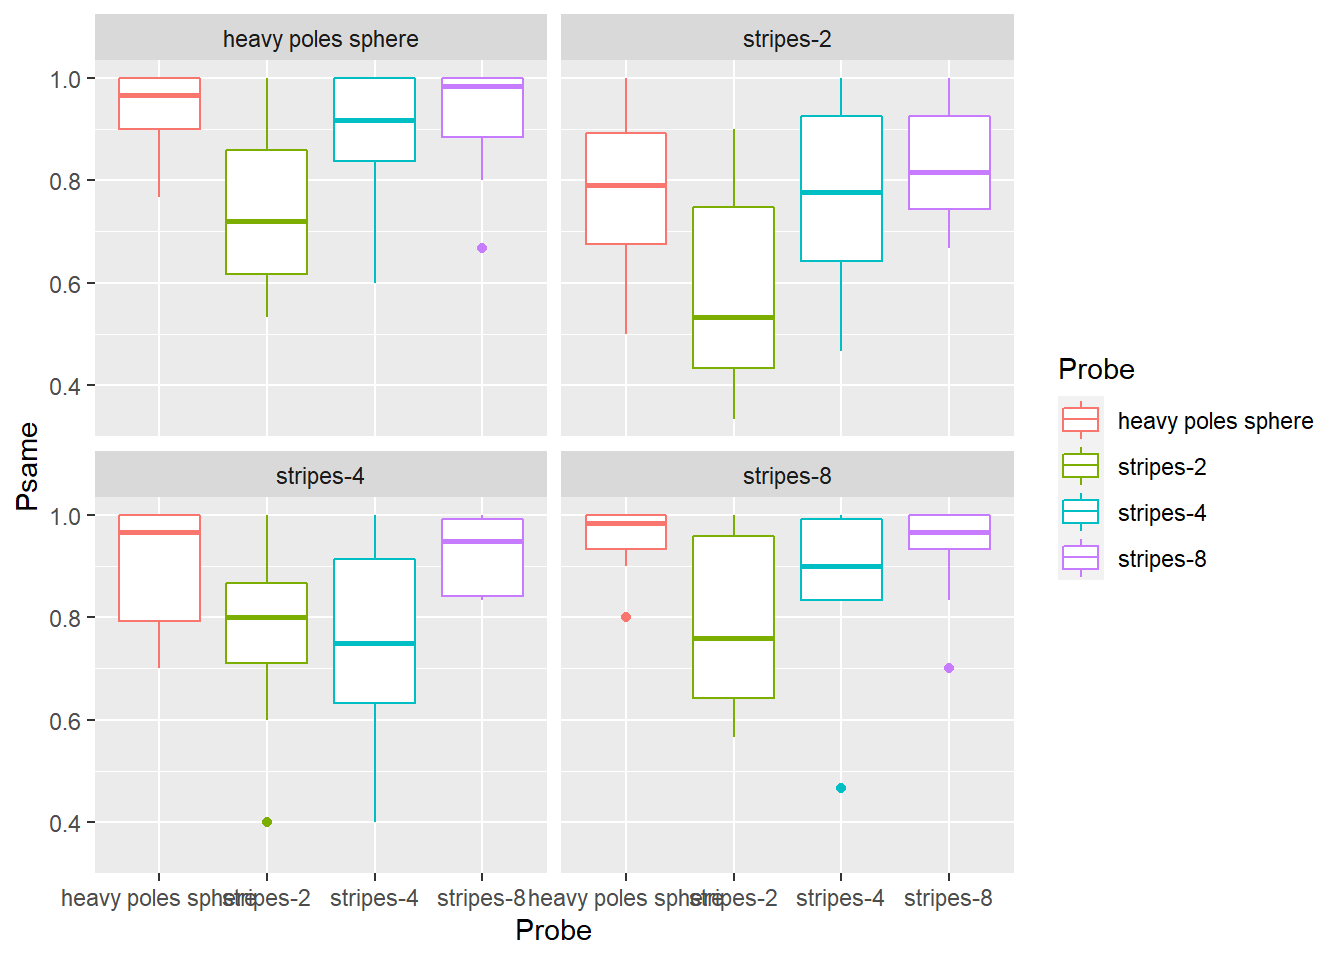
\includegraphics{data-analysis-using-r-for-psychology_files/figure-latex/unnamed-chunk-152-1} \end{center}

Do exercise 1.

When you examine the plot, you can see some sort of non-monotonic dependence with a dip for \texttt{"stripes-2"} and \texttt{"stripes-4"} objects. In reality, the dependence is monotonic, it is merely the order of values on the x-axis that is wrong. The correct order, based on the area of an object covered with dots, is \texttt{"heavy\ poles\ sphere"}, \texttt{"stripes-8"}, \texttt{"stripes-4"}, \texttt{"stripes-2"}. Both \texttt{Prime} and \texttt{Probe} are \emph{ordinal} variables called \emph{factors} in R. Thus, to fix the order and to make object names a bit better looking, we must figure out how to work with factors in R.

\hypertarget{factors}{%
\section{Factors}\label{factors}}

Factors are categorical variables, thus variables that have a finite fixed and known set of possible values. They can be either \emph{nominal} (cannot be ordered) or \emph{ordinal} (have a specific order to them). An example of the former is the drive train (\texttt{drv}) variable in \href{https://ggplot2.tidyverse.org/reference/mpg.html}{mpg} table. There is a finite set of possible values (\texttt{"f"} for front-wheel drive, \texttt{"r"} for rear wheel drive, and \texttt{"4"} for a four-wheel drive) but ordering them makes no sense. An example of an ordinal variable is a Likert scale that has a finite set of possible responses (for example, \texttt{"disagree"}, \texttt{"neither\ agree,\ nor\ disagree"}, \texttt{"agree"}) with a specific fixed order (participant's support for a statement is progressively stronger so that \texttt{"disagree"} \textless{} \texttt{"neither\ agree,\ nor\ disagree"} \textless{} \texttt{"agree"}).

You can convert \emph{any} variable to a factor using \href{https://stat.ethz.ch/R-manual/R-devel/library/base/html/factor.html}{factor()} or \texttt{as.factor()} functions. The latter is a more limited version of the former, so it makes little sense to ever use it. Below, I will only use \href{https://stat.ethz.ch/R-manual/R-devel/library/base/html/factor.html}{factor()}. When you convert a variable (a vector) to factor, R:

\begin{enumerate}
\def\labelenumi{\arabic{enumi}.}
\tightlist
\item
  figures out all \href{https://stat.ethz.ch/R-manual/R-devel/library/base/html/unique.html}{unique} values in this vector
\item
  sorts them in an ascending order
\item
  assigns each value an integer index, a.k.a. ``level''
\item
  uses the actual value as a ``label''.
\end{enumerate}

Here is an example of this sequence: there four levels sorted alphabetically (note that R prints out not only the vector but also its levels).

\begin{Shaded}
\begin{Highlighting}[]
\NormalTok{letters }\OtherTok{\textless{}{-}} \FunctionTok{c}\NormalTok{(}\StringTok{"C"}\NormalTok{, }\StringTok{"A"}\NormalTok{, }\StringTok{"D"}\NormalTok{, }\StringTok{"B"}\NormalTok{, }\StringTok{"A"}\NormalTok{, }\StringTok{"B"}\NormalTok{)}
\NormalTok{letters\_as\_factor }\OtherTok{\textless{}{-}} \FunctionTok{factor}\NormalTok{(letters)}
\NormalTok{letters\_as\_factor}
\end{Highlighting}
\end{Shaded}

\begin{verbatim}
## [1] C A D B A B
## Levels: A B C D
\end{verbatim}

You can extracts \href{https://stat.ethz.ch/R-manual/R-devel/library/base/html/levels.html}{levels} of a factor variable by using the function of the same name

\begin{Shaded}
\begin{Highlighting}[]
\FunctionTok{levels}\NormalTok{(letters\_as\_factor)}
\end{Highlighting}
\end{Shaded}

\begin{verbatim}
## [1] "A" "B" "C" "D"
\end{verbatim}

You can specify the order of levels either during the \href{https://stat.ethz.ch/R-manual/R-devel/library/base/html/factor.html}{factor()} call or later using \href{https://forcats.tidyverse.org/}{forcats} library (more on that later). For example, if we want to have levels in the reverse order we specify it via \texttt{levels} parameter. Note the opposite order of levels.

\begin{Shaded}
\begin{Highlighting}[]
\NormalTok{letters }\OtherTok{\textless{}{-}} \FunctionTok{c}\NormalTok{(}\StringTok{"C"}\NormalTok{, }\StringTok{"A"}\NormalTok{, }\StringTok{"D"}\NormalTok{, }\StringTok{"B"}\NormalTok{, }\StringTok{"A"}\NormalTok{, }\StringTok{"B"}\NormalTok{)}
\NormalTok{letters\_as\_factor }\OtherTok{\textless{}{-}} \FunctionTok{factor}\NormalTok{(letters, }\AttributeTok{levels =} \FunctionTok{c}\NormalTok{(}\StringTok{"D"}\NormalTok{, }\StringTok{"C"}\NormalTok{, }\StringTok{"B"}\NormalTok{, }\StringTok{"A"}\NormalTok{))}
\NormalTok{letters\_as\_factor}
\end{Highlighting}
\end{Shaded}

\begin{verbatim}
## [1] C A D B A B
## Levels: D C B A
\end{verbatim}

We can also specify \texttt{labels} of individual labels instead of using values themselves. Note that the labels must match levels in \emph{number} and \emph{order}.

\begin{Shaded}
\begin{Highlighting}[]
\NormalTok{responses }\OtherTok{\textless{}{-}} \FunctionTok{c}\NormalTok{(}\DecValTok{1}\NormalTok{, }\DecValTok{3}\NormalTok{, }\DecValTok{2}\NormalTok{, }\DecValTok{2}\NormalTok{, }\DecValTok{1}\NormalTok{, }\DecValTok{3}\NormalTok{)}
\NormalTok{responses\_as\_factor }\OtherTok{\textless{}{-}} \FunctionTok{factor}\NormalTok{(responses, }\AttributeTok{levels =} \FunctionTok{c}\NormalTok{(}\DecValTok{1}\NormalTok{, }\DecValTok{2}\NormalTok{, }\DecValTok{3}\NormalTok{), }\AttributeTok{labels =} \FunctionTok{c}\NormalTok{(}\StringTok{"negative"}\NormalTok{, }\StringTok{"neutral"}\NormalTok{, }\StringTok{"positive"}\NormalTok{))}
\NormalTok{responses\_as\_factor}
\end{Highlighting}
\end{Shaded}

\begin{verbatim}
## [1] negative positive neutral  neutral  negative positive
## Levels: negative neutral positive
\end{verbatim}

You can see \emph{indexes} that were assigned to each level by converting \texttt{letter\_as\_factor} to a numeric vector. In this case, R throws away labels and returns indexes.

\begin{Shaded}
\begin{Highlighting}[]
\FunctionTok{as.numeric}\NormalTok{(letters\_as\_factor)}
\end{Highlighting}
\end{Shaded}

\begin{verbatim}
## [1] 2 4 1 3 4 3
\end{verbatim}

However, be careful when level labels are numbers. In the example below, you might think that \texttt{as.numeric(tens)} should give you \texttt{{[}20,\ 40,\ 30{]}}\footnote{At least I tend to always think that.} but these are labels! If you need to convert labels to numbers, you have to do it in two steps \texttt{as.numeric(as.character(tens))}: \texttt{as.character()} turns factors to strings (using labels) and \texttt{as.numeric()} converts those labels to numbers (if that conversion can work).

\begin{Shaded}
\begin{Highlighting}[]
\NormalTok{tens }\OtherTok{\textless{}{-}} \FunctionTok{factor}\NormalTok{(}\FunctionTok{c}\NormalTok{(}\DecValTok{20}\NormalTok{, }\DecValTok{40}\NormalTok{, }\DecValTok{30}\NormalTok{))}
\FunctionTok{print}\NormalTok{(tens)}
\end{Highlighting}
\end{Shaded}

\begin{verbatim}
## [1] 20 40 30
## Levels: 20 30 40
\end{verbatim}

\begin{Shaded}
\begin{Highlighting}[]
\FunctionTok{print}\NormalTok{(}\FunctionTok{as.numeric}\NormalTok{(tens))}
\end{Highlighting}
\end{Shaded}

\begin{verbatim}
## [1] 1 3 2
\end{verbatim}

\begin{Shaded}
\begin{Highlighting}[]
\FunctionTok{print}\NormalTok{(}\FunctionTok{as.numeric}\NormalTok{(}\FunctionTok{as.character}\NormalTok{(tens)))}
\end{Highlighting}
\end{Shaded}

\begin{verbatim}
## [1] 20 40 30
\end{verbatim}

For the next exercise, copy-paste the code from exercise \#1 and alter it so the labels are \texttt{"sphere"} (for \texttt{"heavy\ poles\ sphere"}), \texttt{"quad\ band"} (for \texttt{"stripes-8"}), \texttt{"dual\ band"} (\texttt{"stripes-4"}), \texttt{"single\ band"} (for \texttt{"stripes-2"}) and levels are in that order. Your plot should look something like this.

\begin{center}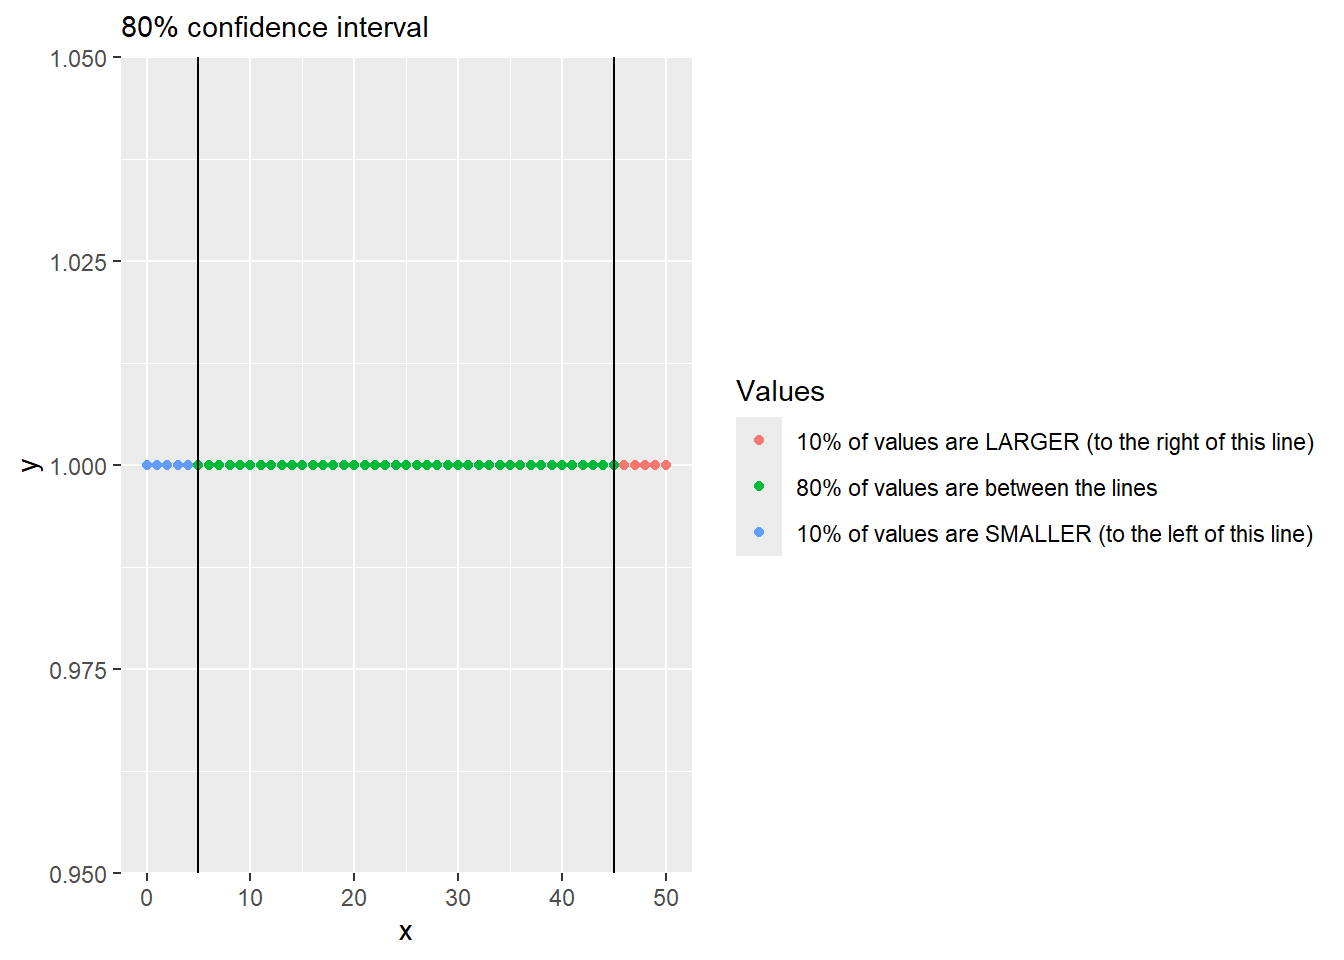
\includegraphics{data-analysis-using-r-for-psychology_files/figure-latex/unnamed-chunk-159-1} \end{center}

Do exercise 2.

\hypertarget{forcats}{%
\section{Forcats}\label{forcats}}

Tidyverse has a package \href{https://forcats.tidyverse.org/}{forcats}\footnote{The package's name is anagram of \emph{factors}.} that makes working with factors easier. For example, it allows to reorder levels either \href{https://forcats.tidyverse.org/reference/fct_relevel.html}{by hand} or automatically based on the \href{https://forcats.tidyverse.org/reference/fct_inorder.html}{order of appearance}, \href{https://forcats.tidyverse.org/reference/fct_inorder.html}{frequency}, \href{https://forcats.tidyverse.org/reference/fct_reorder.html}{value of other variable}, etc. It also gives you flexible tools to changes labels either \href{https://forcats.tidyverse.org/reference/fct_recode.html}{by hand}, by \href{https://forcats.tidyverse.org/reference/fct_lump.html}{lumping} some levels together, by \href{https://forcats.tidyverse.org/reference/fct_anon.html}{anonymising them}, etc. In my work, I mostly use reordering (\href{https://forcats.tidyverse.org/reference/fct_relevel.html}{fct\_relevel()}) and renaming (\href{https://forcats.tidyverse.org/reference/fct_recode.html}{fct\_recode()}) of factors by hand. You will need to use these two functions in exercise \#3. However, if you find yourself working with factors, it is a good idea to check other \href{https://forcats.tidyverse.org/}{forcats} functions to see whether they can make your life easier.

To reorder factor by hand, you simply state the desired order of factors, similar to they way you specify this via \texttt{levels=} parameters in \texttt{factor()} function. However, in \href{https://forcats.tidyverse.org/reference/fct_relevel.html}{fct\_relevel()} you can move only \emph{some} factors and others are ``pushed to the back''.

\begin{Shaded}
\begin{Highlighting}[]
\NormalTok{letters }\OtherTok{\textless{}{-}} \FunctionTok{c}\NormalTok{(}\StringTok{"C"}\NormalTok{, }\StringTok{"A"}\NormalTok{, }\StringTok{"D"}\NormalTok{, }\StringTok{"B"}\NormalTok{, }\StringTok{"A"}\NormalTok{, }\StringTok{"B"}\NormalTok{)}
\NormalTok{letters\_as\_factor }\OtherTok{\textless{}{-}} \FunctionTok{factor}\NormalTok{(letters, }\AttributeTok{levels =} \FunctionTok{c}\NormalTok{(}\StringTok{"B"}\NormalTok{, }\StringTok{"C"}\NormalTok{, }\StringTok{"D"}\NormalTok{, }\StringTok{"A"}\NormalTok{))}
\FunctionTok{print}\NormalTok{(letters\_as\_factor)}
\end{Highlighting}
\end{Shaded}

\begin{verbatim}
## [1] C A D B A B
## Levels: B C D A
\end{verbatim}

\begin{Shaded}
\begin{Highlighting}[]
\CommentTok{\# specifying order for ALL levels}
\NormalTok{letters\_as\_factor }\OtherTok{\textless{}{-}} \FunctionTok{fct\_relevel}\NormalTok{(letters\_as\_factor, }\StringTok{"D"}\NormalTok{, }\StringTok{"C"}\NormalTok{, }\StringTok{"B"}\NormalTok{, }\StringTok{"A"}\NormalTok{)}
\FunctionTok{print}\NormalTok{(letters\_as\_factor)}
\end{Highlighting}
\end{Shaded}

\begin{verbatim}
## [1] C A D B A B
## Levels: D C B A
\end{verbatim}

\begin{Shaded}
\begin{Highlighting}[]
\CommentTok{\# specifying order for just ONE level, the rest are "pushed back"}
\CommentTok{\# "A" should now be the first level and the rest are pushed back in their original order}
\NormalTok{letters\_as\_factor }\OtherTok{\textless{}{-}} \FunctionTok{fct\_relevel}\NormalTok{(letters\_as\_factor, }\StringTok{"A"}\NormalTok{)}
\FunctionTok{print}\NormalTok{(letters\_as\_factor)}
\end{Highlighting}
\end{Shaded}

\begin{verbatim}
## [1] C A D B A B
## Levels: A D C B
\end{verbatim}

You can also put a level at the very back, as second level, etc. \href{https://forcats.tidyverse.org/reference/fct_relevel.html}{fct\_relevel()} is very flexible, so check reference whenever you use it.

To rename individual levels you use \href{https://forcats.tidyverse.org/reference/fct_recode.html}{fct\_recode()} by providing \texttt{new\ =\ old} pairs of values.

\begin{Shaded}
\begin{Highlighting}[]
\NormalTok{letters\_as\_factor }\OtherTok{\textless{}{-}} \FunctionTok{factor}\NormalTok{(}\FunctionTok{c}\NormalTok{(}\StringTok{"C"}\NormalTok{, }\StringTok{"A"}\NormalTok{, }\StringTok{"D"}\NormalTok{, }\StringTok{"B"}\NormalTok{, }\StringTok{"A"}\NormalTok{, }\StringTok{"B"}\NormalTok{))}
\NormalTok{letters\_as\_factor }\OtherTok{\textless{}{-}} \FunctionTok{fct\_recode}\NormalTok{(letters\_as\_factor, }\StringTok{"\_A\_"} \OtherTok{=} \StringTok{"A"}\NormalTok{, }\StringTok{"\_C\_"} \OtherTok{=} \StringTok{"C"}\NormalTok{)}
\FunctionTok{print}\NormalTok{(letters\_as\_factor)}
\end{Highlighting}
\end{Shaded}

\begin{verbatim}
## [1] _C_ _A_ D   B   _A_ B  
## Levels: _A_ B _C_ D
\end{verbatim}

Note that this allows you to merge levels by hand.

\begin{Shaded}
\begin{Highlighting}[]
\NormalTok{letters\_as\_factor }\OtherTok{\textless{}{-}} \FunctionTok{factor}\NormalTok{(}\FunctionTok{c}\NormalTok{(}\StringTok{"C"}\NormalTok{, }\StringTok{"A"}\NormalTok{, }\StringTok{"D"}\NormalTok{, }\StringTok{"B"}\NormalTok{, }\StringTok{"A"}\NormalTok{, }\StringTok{"B"}\NormalTok{))}
\NormalTok{letters\_as\_factor }\OtherTok{\textless{}{-}} \FunctionTok{fct\_recode}\NormalTok{(letters\_as\_factor, }\StringTok{"\_AC\_"} \OtherTok{=} \StringTok{"A"}\NormalTok{, }\StringTok{"\_AC\_"} \OtherTok{=} \StringTok{"C"}\NormalTok{)}
\FunctionTok{print}\NormalTok{(letters\_as\_factor)}
\end{Highlighting}
\end{Shaded}

\begin{verbatim}
## [1] _AC_ _AC_ D    B    _AC_ B   
## Levels: _AC_ B D
\end{verbatim}

For exercise \#3, redo exercise \#2 but using \href{https://forcats.tidyverse.org/reference/fct_relevel.html}{fct\_relevel()} and \href{https://forcats.tidyverse.org/reference/fct_recode.html}{fct\_recode()}. You still need to use \texttt{factor()} function to convert \texttt{Prime} and \texttt{Probe} to factor but do not specify levels and labels. Use \href{https://forcats.tidyverse.org/reference/fct_relevel.html}{fct\_relevel()} and \href{https://forcats.tidyverse.org/reference/fct_recode.html}{fct\_recode()} inside \href{https://dplyr.tidyverse.org/reference/mutate.html}{mutate()} verbs to reorder and relabel factor values (or, first relabel and then reorder, whatever is more intuitive for you). The end product (the plot) should be the same.

Do exercise 3.

\hypertarget{plotting-group-averages}{%
\section{Plotting group averages}\label{plotting-group-averages}}

Let us keep practicing and extend our analysis to compute and plots averages for each condition (\texttt{Prime}×\texttt{Probe}) over all participants. Use preprocessing code from exercise \#3 but, once you compute a proportion per \texttt{Participant}×\texttt{Prime}×\texttt{Probe}, you need to group data over \texttt{Prime}×\texttt{Probe} to compute average performance across observers. Advice, \emph{do not} reuse the name of the column, e.g., if you used \texttt{Psame} for proportion per \texttt{Participant}×\texttt{Prime}×\texttt{Probe}, use some \emph{other} name for \texttt{Prime}×\texttt{Probe} (e.g.~\texttt{Pavg}). Otherwise, it may turn out to be very confusing (at least, this is a mistake a make routinely). Take a look at the code below, what will the \texttt{Range} values be?

\begin{Shaded}
\begin{Highlighting}[]
\FunctionTok{tibble}\NormalTok{(}\AttributeTok{ID =} \FunctionTok{c}\NormalTok{(}\StringTok{"A"}\NormalTok{, }\StringTok{"A"}\NormalTok{, }\StringTok{"B"}\NormalTok{, }\StringTok{"B"}\NormalTok{),}
       \AttributeTok{Response =} \FunctionTok{c}\NormalTok{(}\DecValTok{1}\NormalTok{, }\DecValTok{2}\NormalTok{, }\DecValTok{4}\NormalTok{, }\DecValTok{6}\NormalTok{)) }\SpecialCharTok{\%\textgreater{}\%}
  
  \FunctionTok{group\_by}\NormalTok{(ID) }\SpecialCharTok{\%\textgreater{}\%}
  \FunctionTok{summarise}\NormalTok{(}\AttributeTok{Response =} \FunctionTok{mean}\NormalTok{(Response),}
            \AttributeTok{Range =} \FunctionTok{max}\NormalTok{(Response) }\SpecialCharTok{{-}} \FunctionTok{min}\NormalTok{(Response))}
\end{Highlighting}
\end{Shaded}

I routinely assume that they should be \texttt{1} for \texttt{"A"} (because \texttt{2-1}) and \texttt{2} for \texttt{"B"} (\texttt{6-4}). Nope, both are \texttt{0} because by the time \texttt{Range\ =\ max(Response)\ -\ min(Response)} is executed, original values of \texttt{Response} are overwritten by \texttt{Response\ =\ mean(Response)}, so it has just \textbf{one} value, the mean. And \texttt{min()} and \texttt{max()} of a single value is that value, so their difference is \texttt{0}. It is obvious once you carefully consider the code but it is \emph{not} obvious (at least to me) straightaway. In short, be \textbf{very careful} when you are reusing column names. Better still, do not reuse them, be creative, come up with new ones!

Getting back to the exercise, compute average performance per \texttt{Prime}×\texttt{Probe}. Store the result of the computation in a new variable (I've called it \texttt{persistence\_avg}) and check that results makes sense, e.g.~you have just three columns \texttt{Prime}, \texttt{Probe}, and \texttt{Pavg} (or however you decided to name the column). They should look like this:

\begin{tabular}{l|l|r}
\hline
Prime & Probe & Pavg\\
\hline
sphere & sphere & 0.9366667\\
\hline
sphere & quad band & 0.9233333\\
\hline
sphere & dual band & 0.8885185\\
\hline
sphere & single band & 0.7507407\\
\hline
quad band & sphere & 0.9533333\\
\hline
quad band & quad band & 0.9333333\\
\hline
quad band & dual band & 0.8729630\\
\hline
quad band & single band & 0.7885185\\
\hline
dual band & sphere & 0.9033333\\
\hline
dual band & quad band & 0.9229630\\
\hline
dual band & dual band & 0.7418519\\
\hline
dual band & single band & 0.7707407\\
\hline
single band & sphere & 0.7814815\\
\hline
single band & quad band & 0.8311111\\
\hline
single band & dual band & 0.7751852\\
\hline
single band & single band & 0.5792593\\
\hline
\end{tabular}

Do exercise 4.

Then, plot the results. Use \href{https://ggplot2.tidyverse.org/reference/geom_point.html}{geom\_point()} plus \href{https://ggplot2.tidyverse.org/reference/geom_path.html}{geom\_line()} to plot the mean response The plot should like like this (hint, drop color mapping and map \texttt{Prime} to \texttt{group} property).

\begin{center}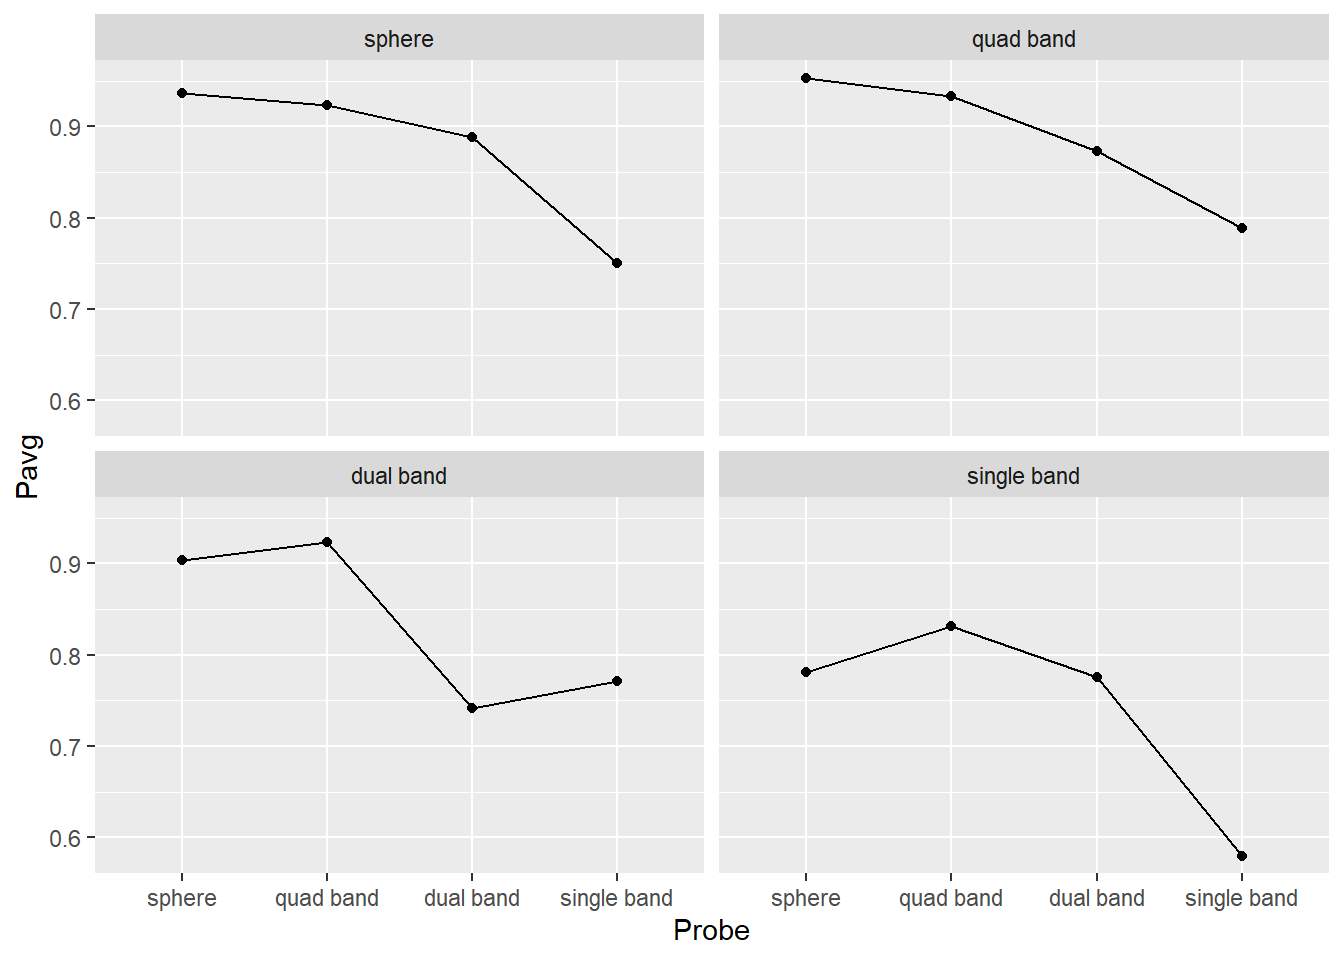
\includegraphics{data-analysis-using-r-for-psychology_files/figure-latex/unnamed-chunk-167-1} \end{center}

Do exercise 5.

Tweak code from exercise 4 to plot all lines on the same plot and use color property to distinguish between different primes.

\begin{center}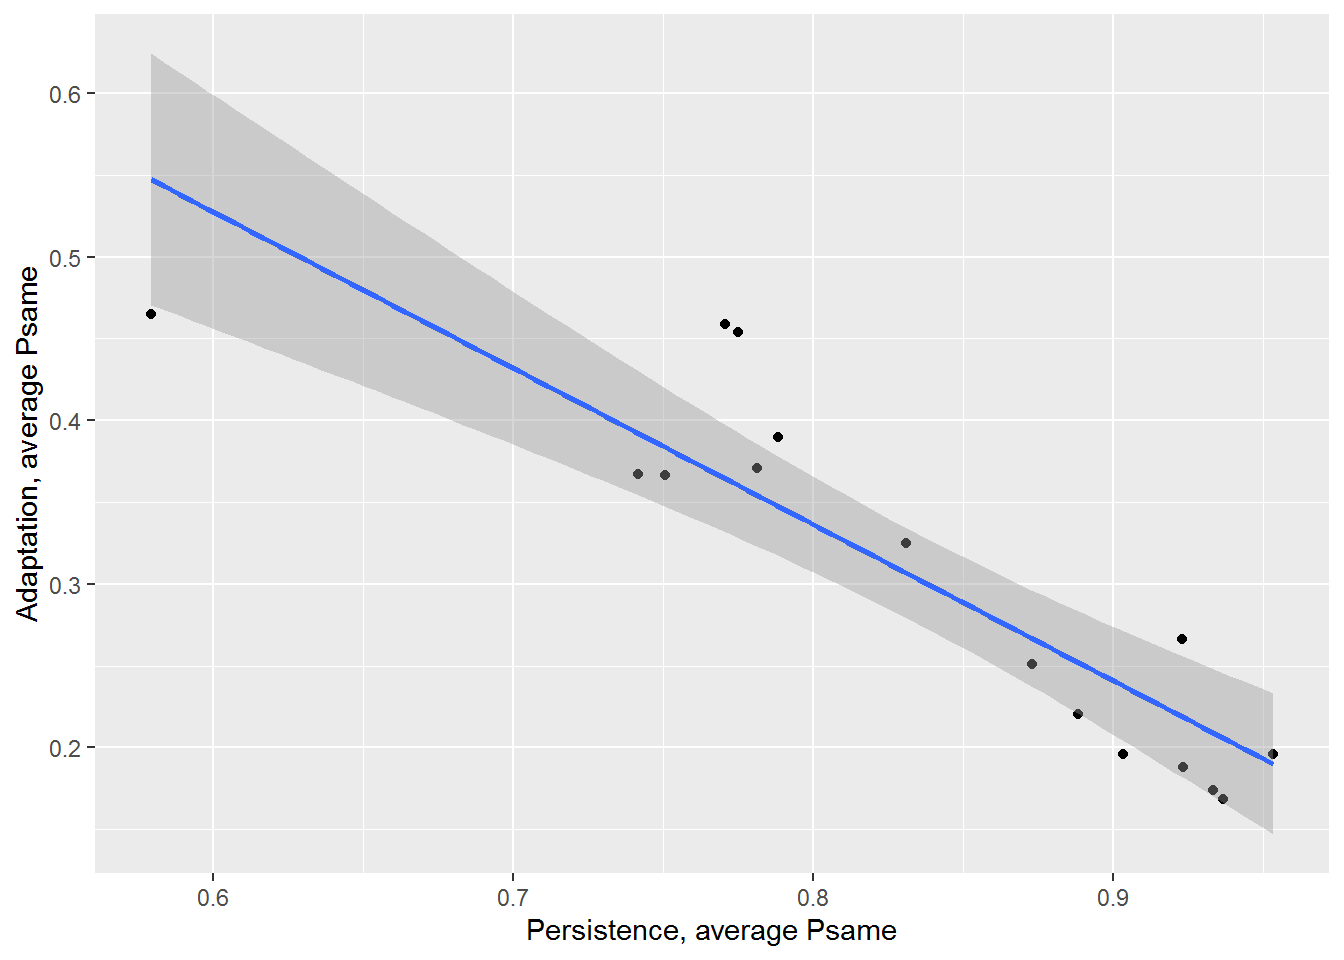
\includegraphics{data-analysis-using-r-for-psychology_files/figure-latex/unnamed-chunk-168-1} \end{center}

Do exercise 6.

\hypertarget{plotting-our-confidence-in-group-averages-via-quantiles}{%
\section{Plotting our confidence in group averages via quantiles}\label{plotting-our-confidence-in-group-averages-via-quantiles}}

From the plots above, you get a sense that identities of the probe and prime (objects before and after the interruption) matter. Single band appears to be the poorest prime (its line is lowest) and probe (its dots are lower than the rest). Conversely, sphere is an excellent prime (line at the top) and probe (dots are very high). However, averages that we plotted is just a point estimate for most likely effect strength but they alone cannot tell us whether differences in objects' shape do matter. For this, you need to perform statistical analysis but to get at least a feeling of how confident can you be about these differences, you need to plot a measure of variability associated with that \emph{statistics}. I.e., \texttt{{[}1,\ 5,\ 9{]}} and \texttt{{[}4,\ 5,\ 6{]}} both have identical mean of 5 but their standard deviation is 4.5 \emph{times} different (4.51 vs.~1). In the second case, the true mean is likely to be somewhere very near to 5, whereas we would have much less confidence in the former one.

One way to characterize the mean is by computing its \href{https://en.wikipedia.org/wiki/Standard_error}{standard error}. However, it is best used when actual data is distributed normally or, at least, symmetrically around the mean, i.e., the distance from an observation to the mean could be the same irrespective of whether it is larger or smaller. This is a luxury you can expect only for variables that live on ±∞ range (support) or if the practically observed range of values is very far from either the floor or the ceiling. Adult height is an example of the latter: You cannot have height below 0 but an average adult height is far enough from that limit so its distribution is normal and symmetric enough. Unfortunately, a lot of data that we collect in psychology or social science research does not fit this description: Binomial data with yes/no or correct/incorrect responses lives on 0..1 range, response times have long right tail because they cannot be negative or even particularly short (200 ms would be a realistic floor for key presses, \textasciitilde120 ms for eye saccadic response under \emph{very} specific experimental conditions.)\footnote{I did not mention Likert scale data because it is an ordered categorical type data, so you cannot use raw data to compute even the mean, let alone its error.}

In our case the outcome variable is a \emph{proportion} limited to 0 to 1 range. From practical point of view this means that our measure of variability is unlikely to be symmetric relative to the mean (with a unique exception of the mean exactly 0.5). I.e., think about a group average \(P_{avg} = 0.8\), points \emph{below} that average can be further away from the mean (up to 0.8) than points \emph{above} it (0.2 away at most). This compression is called either a ceiling (when you get squashed by the upper range) or flooring (when you cannot go below certain value) effect. Thus, we need a measure that would take this asymmetry into account. Later on you will learn how to do it using bootstrapping but we will start with a simpler approach of just using \href{https://en.wikipedia.org/wiki/Quantile}{quantiles} of a distribution to understand its variability.

To compute this quantiles-based interval, you need to compute its lower and upper limits separately via \href{https://en.wikipedia.org/wiki/Quantile}{quantiles}. A quantile for 0.1 (10\%) returns a value, so that 10\% of all values in the vector are below it, the quantile of 0.9 (90\%) means that only 10\% of values are above it (or 90\% are below). So, an 80\% confidence intervals includes values that are between 10\% and 90\% or, alternatively, between 0.1 and 0.9 quantiles.

\begin{center}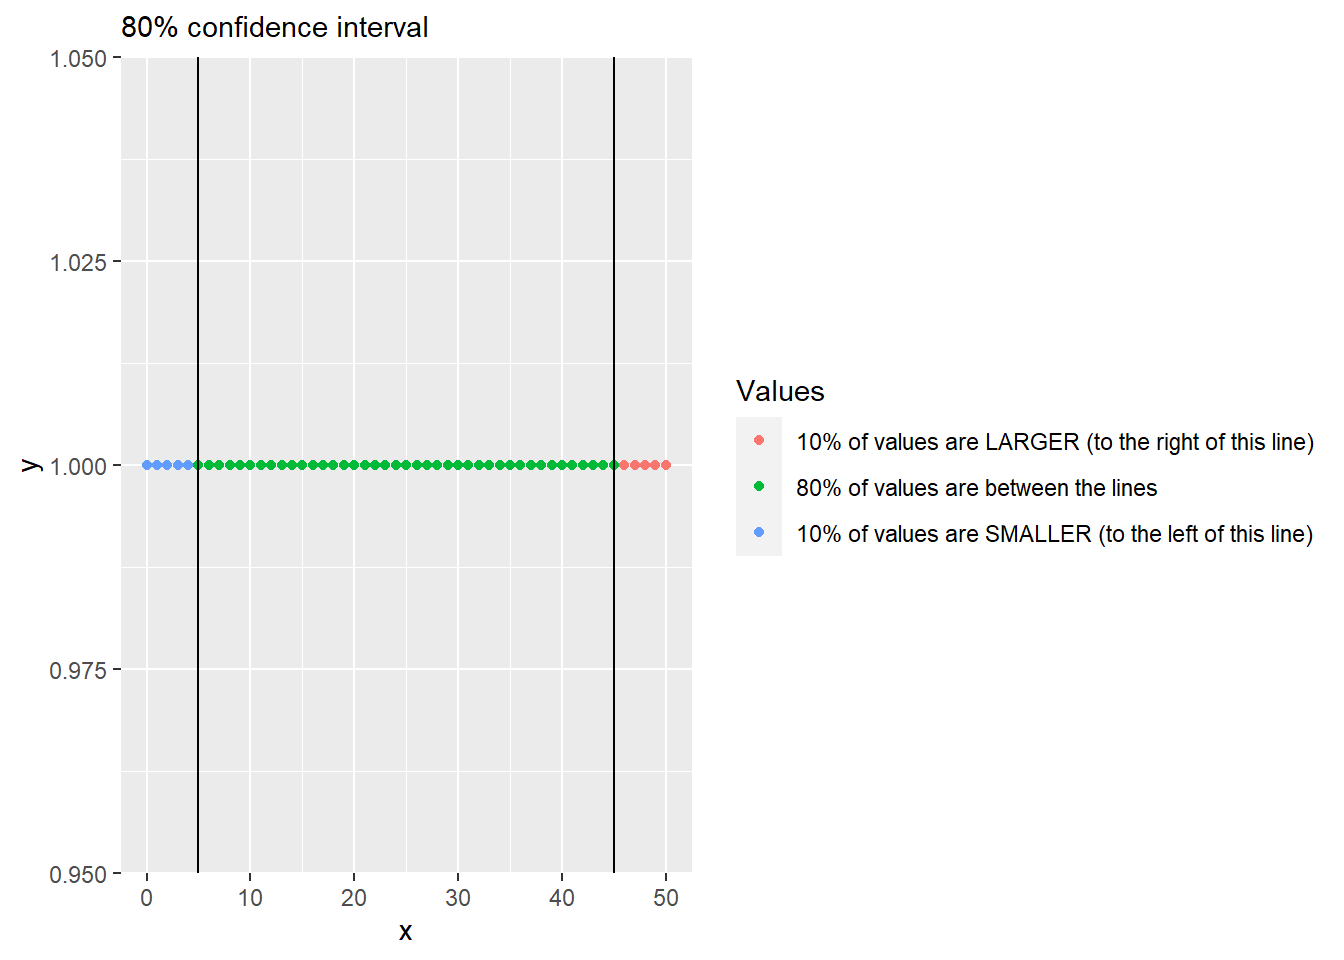
\includegraphics[width=1\linewidth]{data-analysis-using-r-for-psychology_files/figure-latex/unnamed-chunk-169-1} \end{center}

To compute this, R has function \href{https://stat.ethz.ch/R-manual/R-devel/library/stats/html/quantile.html}{quantile()}.

\begin{Shaded}
\begin{Highlighting}[]
\NormalTok{x }\OtherTok{\textless{}{-}} \DecValTok{0}\SpecialCharTok{:}\DecValTok{50}
\FunctionTok{quantile}\NormalTok{(x, }\FloatTok{0.1}\NormalTok{)}
\end{Highlighting}
\end{Shaded}

\begin{verbatim}
## 10% 
##   5
\end{verbatim}

Modify code from from exercise \#5 to compute two additional variables/columns for lower and upper limits of the \emph{89\%}\footnote{Why 89\%? Because it is a prime number! If you think that it sounds arbitrary, you are perfectly correct. But so is using 95\% and for that one you do not even have the ``prime number'' excuse!} interval (think about what these limits are for 89\% interval). Then, use \href{https://ggplot2.tidyverse.org/reference/geom_linerange.html}{geom\_errorbar()} to plot 89\% interval (you will need to map the two variable you computed to \texttt{ymin} and \texttt{ymax} properties). The plot should look like this (hint, drop color mapping and map \texttt{Prime} to \texttt{group} property).

\begin{center}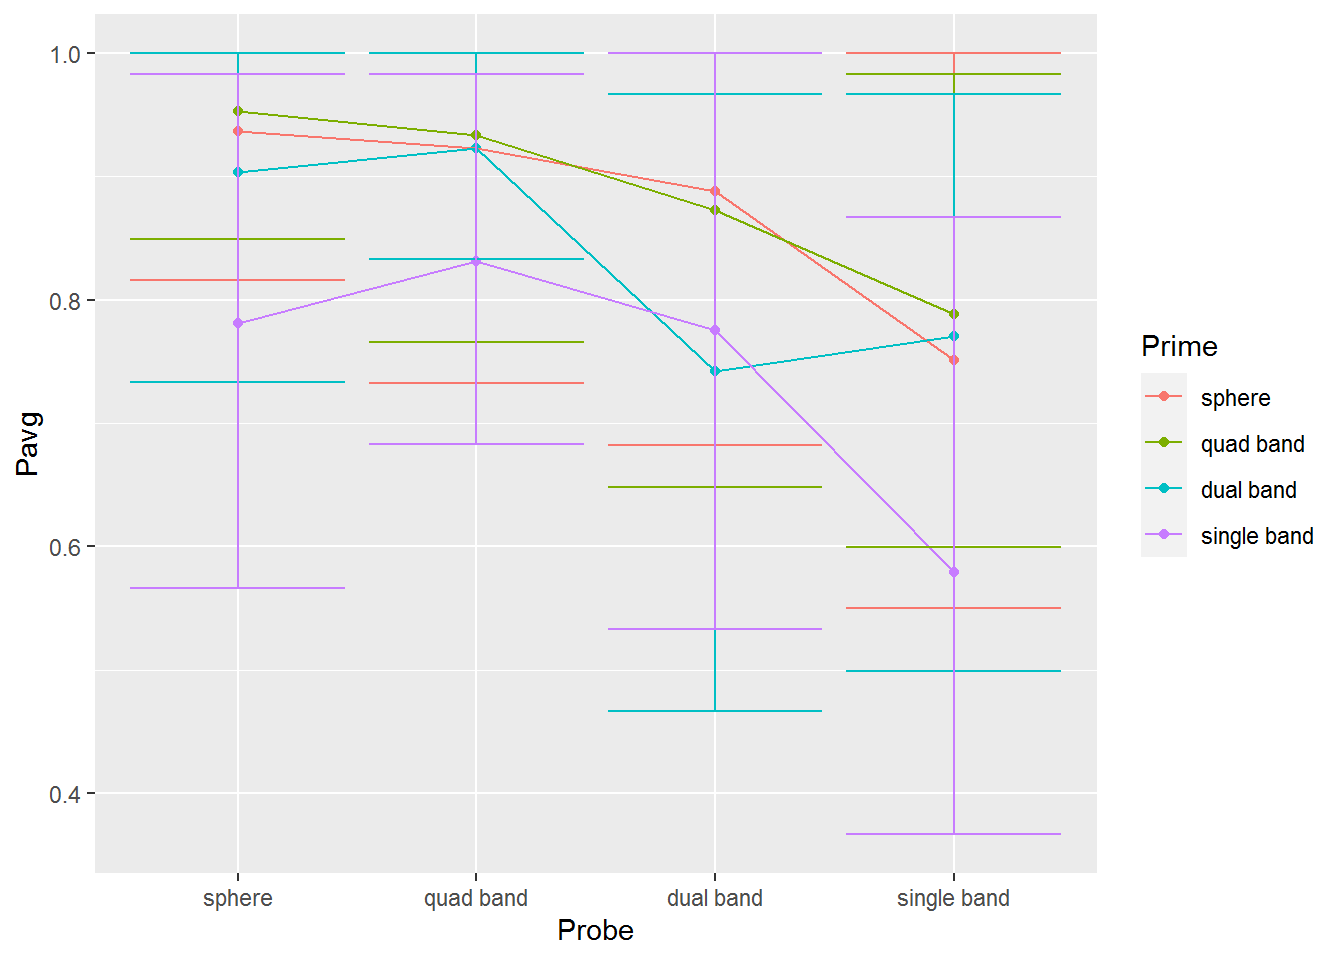
\includegraphics{data-analysis-using-r-for-psychology_files/figure-latex/unnamed-chunk-171-1} \end{center}

Do exercise 7.

\hypertarget{looking-at-similarity}{%
\section{Looking at similarity}\label{looking-at-similarity}}

A different study, which used same four objects, showed that a similar looking history effect but for longer interruptions (1000 ms rather than 50 ms) was modulated by objects similarity. Let us check that hypothesis by computing a rough difference measure. It will assume that their difference is proportional to the absolute ``distance'' between them on x-axis in the above plot\footnote{This measure assumes metric distance, which is a very strong assumption.}. E.g., distance between a sphere and a sphere is 0, but between sphere and quad-band or single-band and dual-band is 1. Difference between sphere and dual-band is 2, etc. You can compute it by converting \emph{factor} variables \texttt{Prime} and \texttt{Probe} to integers (this assumes that levels are in the correct order). Then, you can compute the \href{https://stat.ethz.ch/R-manual/R-devel/library/base/html/MathFun.html}{absolute difference} between those indexes and store it as a new column (e.g.~\texttt{Difference}). Next, group by \texttt{Difference} and \texttt{Participant} to compute average probability of the same response. Your plot should look like this (you will need to map \texttt{Difference} on \texttt{group} to get four box plots rather than one).

\begin{center}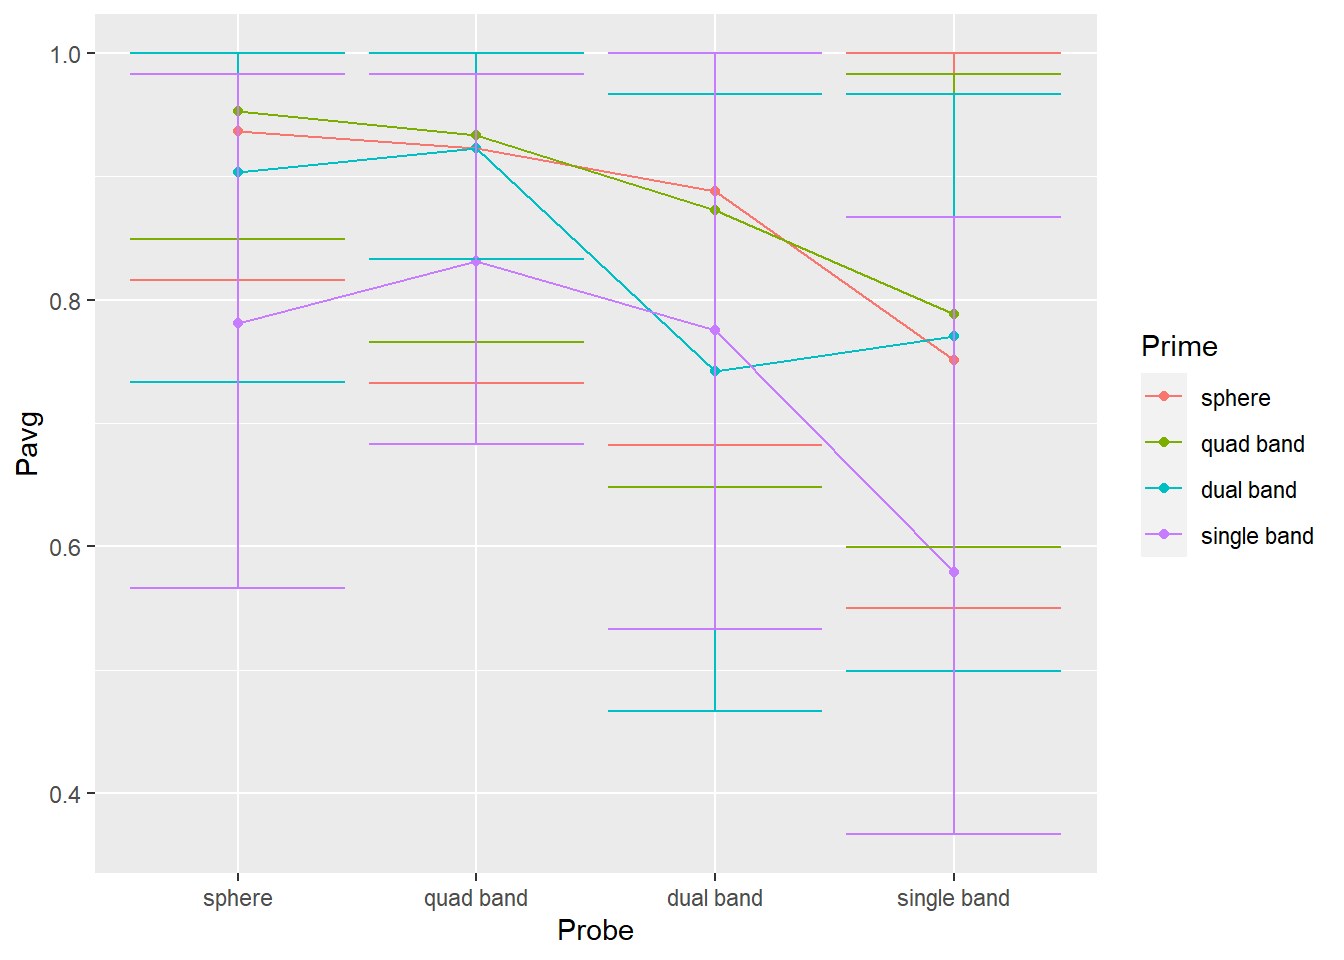
\includegraphics{data-analysis-using-r-for-psychology_files/figure-latex/unnamed-chunk-172-1} \end{center}

Do exercise 8.

\hypertarget{tyding}{%
\chapter{Tidyng your data: joins and pivots}\label{tyding}}

It is fun to work with tidy complete data. Unfortunately, more often than not you will need to preprocess and tidy it up before you can analyze it. In addition to \href{https://dplyr.tidyverse.org/}{dplyr}, Tidyverse has \href{https://tidyr.tidyverse.org/}{tidyr} package that helps you with some of the problems. Grab the \href{notebooks/Seminar\%2008\%20-\%20tidyr.Rmd}{exercise notebook} and let's get started.

\hypertarget{joins}{%
\section{Joining tables}\label{joins}}

Sometimes, results of a study are stored in separate tables. For example, demographic information can be stored separately from responses, as the former is the same for all trials and conditions, so it makes little sense to duplicate it. For the actual analysis, you may eed to add this information, \href{https://stat.ethz.ch/R-manual/R-devel/library/base/html/merge.html}{merging} or, in SQL/Tidyverse-speak, \href{https://dplyr.tidyverse.org/reference/mutate-joins.html}{joining} two tables (I'll use term ``join'' from hereon).

Examples make joining operations much easier to understand, so let us create two tables.

\begin{Shaded}
\begin{Highlighting}[]
\NormalTok{demographics }\OtherTok{\textless{}{-}} \FunctionTok{tibble}\NormalTok{(}\AttributeTok{ID =} \FunctionTok{c}\NormalTok{(}\StringTok{"A"}\NormalTok{, }\StringTok{"B"}\NormalTok{, }\StringTok{"C"}\NormalTok{, }\StringTok{"D"}\NormalTok{),}
                       \AttributeTok{Age =} \FunctionTok{c}\NormalTok{(}\DecValTok{20}\NormalTok{, }\DecValTok{19}\NormalTok{, }\DecValTok{30}\NormalTok{, }\DecValTok{22}\NormalTok{))}
\NormalTok{reports }\OtherTok{\textless{}{-}} 
  \FunctionTok{tibble}\NormalTok{(}\AttributeTok{ID =} \FunctionTok{c}\NormalTok{(}\StringTok{"A"}\NormalTok{, }\StringTok{"B"}\NormalTok{, }\StringTok{"C"}\NormalTok{, }\StringTok{"D"}\NormalTok{, }\StringTok{"A"}\NormalTok{, }\StringTok{"B"}\NormalTok{, }\StringTok{"C"}\NormalTok{, }\StringTok{"D"}\NormalTok{)) }\SpecialCharTok{\%\textgreater{}\%}
  \FunctionTok{mutate}\NormalTok{(}\AttributeTok{Report =} \FunctionTok{runif}\NormalTok{(}\FunctionTok{length}\NormalTok{(ID), }\DecValTok{1}\NormalTok{, }\DecValTok{7}\NormalTok{)) }\SpecialCharTok{\%\textgreater{}\%}
  \FunctionTok{arrange}\NormalTok{(ID)}
\end{Highlighting}
\end{Shaded}

\begin{table}
\caption{\label{tab:unnamed-chunk-175}demographics (left) and report (right) tables}

\centering
\begin{tabular}[t]{l|r}
\hline
ID & Age\\
\hline
A & 20\\
\hline
B & 19\\
\hline
C & 30\\
\hline
D & 22\\
\hline
\end{tabular}
\centering
\begin{tabular}[t]{l|r}
\hline
ID & Report\\
\hline
A & 2.295984\\
\hline
A & 2.457827\\
\hline
B & 6.423922\\
\hline
B & 2.426577\\
\hline
C & 2.797792\\
\hline
C & 3.524973\\
\hline
D & 6.792641\\
\hline
D & 3.066635\\
\hline
\end{tabular}
\end{table}

To join two tables, you require ``key'' columns: columns that contain values that will be used to identify matching rows in the two tables. You can use multiple and differently named columns for that purpose but we will start with a simplest case: a single column with same name \texttt{"ID"}. A \href{https://dplyr.tidyverse.org/reference/mutate-joins.html}{join} function (\texttt{inner\_join()} here, see below for details on different joins) takes a first row in \texttt{demographics} table that has \texttt{"A"} in \texttt{ID} column and will look for all rows in table \texttt{reports} that has \texttt{ID\ ==\ "A"}. Then, it will do the same for all remaining rows for \texttt{demographics} table, one row at a time. It takes three parameters: table \texttt{x} (first table), table \texttt{y} (second table), and \texttt{by} - a vector with key column names argument\footnote{Theoretically, you can skip it and \emph{dplyr} will do its best to find matching columns. However, this is a dangerous thing to leave out, as your intuition and \emph{dlpyr's} matching rules may lead to different results. I strongly recommend to always specify key columns.}. A call to \href{https://stat.ethz.ch/R-manual/R-devel/library/base/html/merge.html}{merge()} function is very similar and produces identical results. Note how column order has changed for \href{https://stat.ethz.ch/R-manual/R-devel/library/base/html/merge.html}{merge()}, because I used a different order of tables, but the content itself is the same.

\begin{Shaded}
\begin{Highlighting}[]
\NormalTok{via\_join }\OtherTok{\textless{}{-}} \FunctionTok{inner\_join}\NormalTok{(demographics, reports, }\AttributeTok{by=}\StringTok{"ID"}\NormalTok{)}
\NormalTok{via\_merge }\OtherTok{\textless{}{-}} \FunctionTok{merge}\NormalTok{(reports, demographics, }\AttributeTok{by=}\StringTok{"ID"}\NormalTok{)}
\end{Highlighting}
\end{Shaded}

\begin{table}
\caption{\label{tab:unnamed-chunk-177}Joining/merging tables with fully matching keys via join (left) and merge (right). Note how a different order of tables results in a different order of columns.}

\centering
\begin{tabular}[t]{l|r|r}
\hline
ID & Age & Report\\
\hline
A & 20 & 2.295984\\
\hline
A & 20 & 2.457827\\
\hline
B & 19 & 6.423922\\
\hline
B & 19 & 2.426577\\
\hline
C & 30 & 2.797792\\
\hline
C & 30 & 3.524973\\
\hline
D & 22 & 6.792641\\
\hline
D & 22 & 3.066635\\
\hline
\end{tabular}
\centering
\begin{tabular}[t]{l|r|r}
\hline
ID & Report & Age\\
\hline
A & 2.295984 & 20\\
\hline
A & 2.457827 & 20\\
\hline
B & 6.423922 & 19\\
\hline
B & 2.426577 & 19\\
\hline
C & 2.797792 & 30\\
\hline
C & 3.524973 & 30\\
\hline
D & 6.792641 & 22\\
\hline
D & 3.066635 & 22\\
\hline
\end{tabular}
\end{table}

Things are easy when every key in the first table has its counterpart in the second one and vice versa. Things get tricky, if that is not the case. Which is why there are \emph{four} different ways to join tables (note that they will all produce identical results for fully matching set of keys, as in the example above):

\begin{itemize}
\tightlist
\item
  \textbf{inner} join: uses only key values that are present in both tables.
\item
  \textbf{full} join: uses all key values from both tables, if matching keys are missing in one of the tables, rows are filled with \texttt{NA}.
\item
  \textbf{left} join: uses only key values that are present in the left (first) table, if matching keys are missing in the \emph{right} table, , rows are filled with \texttt{NA}.
\item
  \textbf{right} join: mirror twin of the left join, uses only key values that are present in the right (second) table, if matching keys are missing in the \emph{left} table, , rows are filled with \texttt{NA}.
\end{itemize}

To see each join in action, let us slightly modify the \texttt{reports} table to include \texttt{ID} ``E'' instead of ``D''. Now, the ``D'' is missing the second table but ``E'' is missing in the \texttt{demographics}:

\begin{Shaded}
\begin{Highlighting}[]
\NormalTok{reports }\OtherTok{\textless{}{-}} 
  \FunctionTok{tibble}\NormalTok{(}\AttributeTok{ID =} \FunctionTok{c}\NormalTok{(}\StringTok{"A"}\NormalTok{, }\StringTok{"B"}\NormalTok{, }\StringTok{"C"}\NormalTok{, }\StringTok{"E"}\NormalTok{, }\StringTok{"A"}\NormalTok{, }\StringTok{"B"}\NormalTok{, }\StringTok{"C"}\NormalTok{, }\StringTok{"E"}\NormalTok{)) }\SpecialCharTok{\%\textgreater{}\%}
  \FunctionTok{mutate}\NormalTok{(}\AttributeTok{Report =} \FunctionTok{runif}\NormalTok{(}\FunctionTok{length}\NormalTok{(ID), }\DecValTok{1}\NormalTok{, }\DecValTok{7}\NormalTok{)) }\SpecialCharTok{\%\textgreater{}\%}
  \FunctionTok{arrange}\NormalTok{(ID)}
\end{Highlighting}
\end{Shaded}

\begin{table}
\caption{\label{tab:unnamed-chunk-179}Now demographics (left) and reports (right) table have unique keys ("D" for demographics, "E" for reports) without a match in the second table.}

\centering
\begin{tabular}[t]{l|r}
\hline
ID & Age\\
\hline
A & 20\\
\hline
B & 19\\
\hline
C & 30\\
\hline
D & 22\\
\hline
\end{tabular}
\centering
\begin{tabular}[t]{l|r}
\hline
ID & Report\\
\hline
A & 4.358237\\
\hline
A & 3.372808\\
\hline
B & 6.500689\\
\hline
B & 4.468184\\
\hline
C & 1.380531\\
\hline
C & 5.587882\\
\hline
E & 3.160737\\
\hline
E & 6.346388\\
\hline
\end{tabular}
\end{table}

\textbf{Inner join} is most conservative and excludes any non-matching keys, note that rows with \emph{both} \texttt{ID\ ==\ "D"} and \texttt{ID\ ==\ "E"} are missing. This is the \emph{default} behavior for the \href{https://stat.ethz.ch/R-manual/R-devel/library/base/html/merge.html}{merge} function.

\begin{Shaded}
\begin{Highlighting}[]
\NormalTok{inner\_tidy }\OtherTok{\textless{}{-}} \FunctionTok{inner\_join}\NormalTok{(reports, demographics, }\AttributeTok{by=}\StringTok{"ID"}\NormalTok{) }
\NormalTok{inner\_base }\OtherTok{\textless{}{-}} \FunctionTok{merge}\NormalTok{(reports, demographics, }\AttributeTok{by=}\StringTok{"ID"}\NormalTok{)}
\end{Highlighting}
\end{Shaded}

\begin{table}

\caption{\label{tab:unnamed-chunk-181}Inner join. Only rows for matching keys are merged}
\centering
\begin{tabular}[t]{l|r|r}
\hline
ID & Report & Age\\
\hline
A & 4.358237 & 20\\
\hline
A & 3.372808 & 20\\
\hline
B & 6.500689 & 19\\
\hline
B & 4.468184 & 19\\
\hline
C & 1.380531 & 30\\
\hline
C & 5.587882 & 30\\
\hline
\end{tabular}
\end{table}

In contrast, \textbf{full join} is the most liberal as it includes all rows from both tables, filling in missing values with \texttt{NA} (e.g., see \texttt{Report} for \texttt{ID\ ==\ "D"} and \texttt{Age} for \texttt{ID\ ==\ "E"}). In base R \href{https://stat.ethz.ch/R-manual/R-devel/library/base/html/merge.html}{merge()} function, you turn an inner join into a full one using \texttt{all=TRUE}.

\begin{Shaded}
\begin{Highlighting}[]
\NormalTok{full\_tidy }\OtherTok{\textless{}{-}} \FunctionTok{full\_join}\NormalTok{(demographics, reports, }\AttributeTok{by=}\StringTok{"ID"}\NormalTok{) }
\NormalTok{full\_base }\OtherTok{\textless{}{-}} \FunctionTok{merge}\NormalTok{(demographics, reports, }\AttributeTok{by=}\StringTok{"ID"}\NormalTok{, }\AttributeTok{all=}\ConstantTok{TRUE}\NormalTok{)}
\end{Highlighting}
\end{Shaded}

\begin{table}

\caption{\label{tab:unnamed-chunk-183}Full join. All rows are merged, `NA` are used for missing values in rows from a complementary table}
\centering
\begin{tabular}[t]{l|r|r}
\hline
ID & Age & Report\\
\hline
A & 20 & 4.358237\\
\hline
A & 20 & 3.372808\\
\hline
B & 19 & 6.500689\\
\hline
B & 19 & 4.468184\\
\hline
C & 30 & 1.380531\\
\hline
C & 30 & 5.587882\\
\hline
D & 22 & NA\\
\hline
E & NA & 3.160737\\
\hline
E & NA & 6.346388\\
\hline
\end{tabular}
\end{table}

\textbf{Left join} uses only rows from the left (first) table, dropping extra rows from the second one. Note \texttt{NA} in \texttt{Report} column for \texttt{ID\ ==\ "D"} and no rows for \texttt{ID\ ==\ "E"}. To do a left join via \href{https://stat.ethz.ch/R-manual/R-devel/library/base/html/merge.html}{merge()}, you need to specify \texttt{all.x=TRUE}.

\begin{Shaded}
\begin{Highlighting}[]
\NormalTok{left\_tidy }\OtherTok{\textless{}{-}} \FunctionTok{left\_join}\NormalTok{(demographics, reports, }\AttributeTok{by=}\StringTok{"ID"}\NormalTok{)}
\NormalTok{left\_base }\OtherTok{\textless{}{-}} \FunctionTok{merge}\NormalTok{(demographics, reports, }\AttributeTok{by=}\StringTok{"ID"}\NormalTok{, }\AttributeTok{all.x=}\ConstantTok{TRUE}\NormalTok{)}
\end{Highlighting}
\end{Shaded}

\begin{table}

\caption{\label{tab:unnamed-chunk-185}Left join. All rows from demographics tables are used and missing matching rows are filled with `NA`}
\centering
\begin{tabular}[t]{l|r|r}
\hline
ID & Age & Report\\
\hline
A & 20 & 4.358237\\
\hline
A & 20 & 3.372808\\
\hline
B & 19 & 6.500689\\
\hline
B & 19 & 4.468184\\
\hline
C & 30 & 1.380531\\
\hline
C & 30 & 5.587882\\
\hline
D & 22 & NA\\
\hline
\end{tabular}
\end{table}

\textbf{Right join} is a mirror twin of the left join, so now rows for \texttt{ID\ ==\ "D"} are missing and there are missing values for \texttt{ID=="E"}. You include \texttt{all.y=TRUE} for a right join via \href{https://stat.ethz.ch/R-manual/R-devel/library/base/html/merge.html}{merge()}.

\begin{Shaded}
\begin{Highlighting}[]
\NormalTok{right\_tidy }\OtherTok{\textless{}{-}} \FunctionTok{right\_join}\NormalTok{(demographics, reports, }\AttributeTok{by=}\StringTok{"ID"}\NormalTok{) }
\NormalTok{right\_base }\OtherTok{\textless{}{-}} \FunctionTok{merge}\NormalTok{(demographics, reports, }\AttributeTok{by=}\StringTok{"ID"}\NormalTok{, }\AttributeTok{all.y=}\ConstantTok{TRUE}\NormalTok{)}
\end{Highlighting}
\end{Shaded}

\begin{table}

\caption{\label{tab:unnamed-chunk-187}Right join. All rows from reports tables are used and missing matching rows are filled with `NA`}
\centering
\begin{tabular}[t]{l|r|r}
\hline
ID & Age & Report\\
\hline
A & 20 & 4.358237\\
\hline
A & 20 & 3.372808\\
\hline
B & 19 & 6.500689\\
\hline
B & 19 & 4.468184\\
\hline
C & 30 & 1.380531\\
\hline
C & 30 & 5.587882\\
\hline
E & NA & 3.160737\\
\hline
E & NA & 6.346388\\
\hline
\end{tabular}
\end{table}

As noted above, you can also use more than one key.

\begin{Shaded}
\begin{Highlighting}[]
\NormalTok{demographics }\OtherTok{\textless{}{-}} \FunctionTok{tibble}\NormalTok{(}\AttributeTok{ID =} \FunctionTok{c}\NormalTok{(}\StringTok{"A"}\NormalTok{, }\StringTok{"B"}\NormalTok{, }\StringTok{"A"}\NormalTok{, }\StringTok{"B"}\NormalTok{),}
                       \AttributeTok{Gender =} \FunctionTok{c}\NormalTok{(}\StringTok{"M"}\NormalTok{, }\StringTok{"F"}\NormalTok{, }\StringTok{"F"}\NormalTok{, }\StringTok{"M"}\NormalTok{),}
                       \AttributeTok{Age =} \FunctionTok{c}\NormalTok{(}\DecValTok{20}\NormalTok{, }\DecValTok{19}\NormalTok{, }\DecValTok{30}\NormalTok{, }\DecValTok{22}\NormalTok{))}
\NormalTok{reports }\OtherTok{\textless{}{-}} \FunctionTok{tibble}\NormalTok{(}\AttributeTok{ID =} \FunctionTok{c}\NormalTok{(}\StringTok{"A"}\NormalTok{, }\StringTok{"B"}\NormalTok{, }\StringTok{"A"}\NormalTok{, }\StringTok{"B"}\NormalTok{),}
                  \AttributeTok{Gender =} \FunctionTok{c}\NormalTok{(}\StringTok{"M"}\NormalTok{, }\StringTok{"F"}\NormalTok{, }\StringTok{"F"}\NormalTok{, }\StringTok{"M"}\NormalTok{),}
                  \AttributeTok{Report =} \FunctionTok{runif}\NormalTok{(}\FunctionTok{length}\NormalTok{(ID), }\DecValTok{1}\NormalTok{, }\DecValTok{7}\NormalTok{))}
\end{Highlighting}
\end{Shaded}

\begin{table}
\caption{\label{tab:unnamed-chunk-189}Two identically named key columns: ID and Gender.}

\centering
\begin{tabular}[t]{l|l|r}
\hline
ID & Gender & Age\\
\hline
A & M & 20\\
\hline
B & F & 19\\
\hline
A & F & 30\\
\hline
B & M & 22\\
\hline
\end{tabular}
\centering
\begin{tabular}[t]{l|l|r}
\hline
ID & Gender & Report\\
\hline
A & M & 1.910337\\
\hline
B & F & 4.210203\\
\hline
A & F & 3.614240\\
\hline
B & M & 4.669292\\
\hline
\end{tabular}
\end{table}

\begin{Shaded}
\begin{Highlighting}[]
\NormalTok{inner\_multi\_tidy }\OtherTok{\textless{}{-}} \FunctionTok{inner\_join}\NormalTok{(demographics, reports, }\AttributeTok{by=}\FunctionTok{c}\NormalTok{(}\StringTok{"ID"}\NormalTok{, }\StringTok{"Gender"}\NormalTok{))}
\NormalTok{inner\_multi\_base }\OtherTok{\textless{}{-}} \FunctionTok{merge}\NormalTok{(demographics, reports, }\AttributeTok{by=}\FunctionTok{c}\NormalTok{(}\StringTok{"ID"}\NormalTok{, }\StringTok{"Gender"}\NormalTok{))}
\end{Highlighting}
\end{Shaded}

\begin{table}

\caption{\label{tab:unnamed-chunk-191}Joining/merging two tables by ID and Gender.}
\centering
\begin{tabular}[t]{l|l|r|r}
\hline
ID & Gender & Age & Report\\
\hline
A & M & 20 & 1.910337\\
\hline
B & F & 19 & 4.210203\\
\hline
A & F & 30 & 3.614240\\
\hline
B & M & 22 & 4.669292\\
\hline
\end{tabular}
\end{table}

Finally, key columns can be named \emph{differently} in two tables. In this case, you need to ``match'' them explicitly. For \href{https://dplyr.tidyverse.org/reference/mutate-joins.html}{dplyr} joins, you use a named vector to match pairs of individual columns. For \href{https://stat.ethz.ch/R-manual/R-devel/library/base/html/merge.html}{merge()}, you supply two vectors: one for columns in the first table (parameter \texttt{by.x}) and one columns in the the second one (parameter \texttt{by.y}). Here, you need to be careful and check that columns order matches in both parameters.

\begin{Shaded}
\begin{Highlighting}[]
\NormalTok{demographics }\OtherTok{\textless{}{-}} \FunctionTok{tibble}\NormalTok{(}\AttributeTok{VPCode =} \FunctionTok{c}\NormalTok{(}\StringTok{"A"}\NormalTok{, }\StringTok{"B"}\NormalTok{, }\StringTok{"A"}\NormalTok{, }\StringTok{"B"}\NormalTok{),}
                       \AttributeTok{Sex =} \FunctionTok{c}\NormalTok{(}\StringTok{"M"}\NormalTok{, }\StringTok{"F"}\NormalTok{, }\StringTok{"F"}\NormalTok{, }\StringTok{"M"}\NormalTok{),}
                       \AttributeTok{Age =} \FunctionTok{c}\NormalTok{(}\DecValTok{20}\NormalTok{, }\DecValTok{19}\NormalTok{, }\DecValTok{30}\NormalTok{, }\DecValTok{22}\NormalTok{))}

\NormalTok{reports }\OtherTok{\textless{}{-}} \FunctionTok{tibble}\NormalTok{(}\AttributeTok{ID =} \FunctionTok{c}\NormalTok{(}\StringTok{"A"}\NormalTok{, }\StringTok{"B"}\NormalTok{, }\StringTok{"A"}\NormalTok{, }\StringTok{"B"}\NormalTok{),}
                  \AttributeTok{Gender =} \FunctionTok{c}\NormalTok{(}\StringTok{"M"}\NormalTok{, }\StringTok{"F"}\NormalTok{, }\StringTok{"F"}\NormalTok{, }\StringTok{"M"}\NormalTok{),}
                  \AttributeTok{Report =} \FunctionTok{runif}\NormalTok{(}\FunctionTok{length}\NormalTok{(ID), }\DecValTok{1}\NormalTok{, }\DecValTok{7}\NormalTok{))}
\end{Highlighting}
\end{Shaded}

\begin{table}
\caption{\label{tab:unnamed-chunk-193}Differently named key columns. VPCode in demographics table corresponds to ID in reports; sex in demographics corresponds to Gender in reports}

\centering
\begin{tabular}[t]{l|l|r}
\hline
VPCode & Sex & Age\\
\hline
A & M & 20\\
\hline
B & F & 19\\
\hline
A & F & 30\\
\hline
B & M & 22\\
\hline
\end{tabular}
\centering
\begin{tabular}[t]{l|l|r}
\hline
ID & Gender & Report\\
\hline
A & M & 1.491876\\
\hline
B & F & 3.677963\\
\hline
A & F & 3.707715\\
\hline
B & M & 1.080628\\
\hline
\end{tabular}
\end{table}

\begin{Shaded}
\begin{Highlighting}[]
\NormalTok{inner\_diff\_tidy }\OtherTok{\textless{}{-}} \FunctionTok{inner\_join}\NormalTok{(demographics, reports, }\AttributeTok{by=}\FunctionTok{c}\NormalTok{(}\StringTok{"VPCode"}\OtherTok{=}\StringTok{"ID"}\NormalTok{, }\StringTok{"Sex"}\OtherTok{=}\StringTok{"Gender"}\NormalTok{))}
\NormalTok{inner\_diff\_base }\OtherTok{\textless{}{-}} \FunctionTok{merge}\NormalTok{(demographics, reports, }\AttributeTok{by.x=}\FunctionTok{c}\NormalTok{(}\StringTok{"VPCode"}\NormalTok{, }\StringTok{"Sex"}\NormalTok{), }\AttributeTok{by.y=}\FunctionTok{c}\NormalTok{(}\StringTok{"ID"}\NormalTok{, }\StringTok{"Gender"}\NormalTok{))}
\end{Highlighting}
\end{Shaded}

\begin{table}

\caption{\label{tab:unnamed-chunk-195}Joining tables by matching VPCode to ID and Sex to Gender.}
\centering
\begin{tabular}[t]{l|l|r|r}
\hline
VPCode & Sex & Age & Report\\
\hline
A & F & 30 & 3.707715\\
\hline
A & M & 20 & 1.491876\\
\hline
B & F & 19 & 3.677963\\
\hline
B & M & 22 & 1.080628\\
\hline
\end{tabular}
\end{table}

As you saw from examples above, \href{https://dplyr.tidyverse.org/reference/mutate-joins.html}{dplyr joins} and \href{https://stat.ethz.ch/R-manual/R-devel/library/base/html/merge.html}{merge()} produce identical results. However, I would recommend to use the former, simply because function names make it explicit which kind of join you perform (something you can figure out only by checking additional parameters of \href{https://stat.ethz.ch/R-manual/R-devel/library/base/html/merge.html}{merge()}).

Download files \href{data/IM.csv}{IM.csv} and \href{data/GP.csv}{GP.csv} that you will need for exercise \#1\footnote{Remember, if you end up with \texttt{.xls} extension, just rename to \texttt{.csv}.}. These are participants responses on two questionnaires with each participant identified by their ID (\texttt{Participant} in \emph{IM.csv} and \texttt{Respondent} in \emph{GP.csv}), \texttt{Condition} (which experimental group they belong to), and their \texttt{Gender}. Read both tables and join them so that there no missing values in the table (some participants are missing in \texttt{GP.csv}, so there are \emph{three} joins that can do this, which one will you pick?). Then, turn \texttt{Condition} and \texttt{Gender} into factors, so that for \texttt{Condition} levels are \texttt{"control"} (\texttt{2}) and \texttt{"game"} (\texttt{1}) and for \texttt{Gender} levels are \texttt{"female"} (\texttt{1}) and \texttt{"male"} (\texttt{2}). Your final table should look as follows (I've dropped most of the columns for \texttt{IM.csv}, so they would fit to the page):

\begin{tabular}{l|l|l|r|r|r|r|r|r|r|r|r|r|r|r|r|r}
\hline
Participant & Condition & Gender & IM01\_01 & IM01\_02 & IM01\_03 & GP01\_01 & GP02\_01 & GP02\_02 & GP02\_03 & GP02\_04 & GP02\_05 & GP02\_06 & GP02\_07 & GP02\_08 & GP02\_09 & GP03\_01\\
\hline
TMM1990w & game & female & 3 & 2 & 5 & 1 & 1 & 1 & 1 & 1 & 6 & 7 & 2 & 1 & 1 & 1\\
\hline
VEH1985w & control & female & 3 & 4 & 4 & 1 & 4 & 4 & 6 & 4 & 6 & 4 & 4 & 4 & 4 & 4\\
\hline
CEN2000w & control & female & 2 & 3 & 6 & 1 & 1 & 1 & 1 & 1 & 4 & 4 & 5 & 4 & 1 & 1\\
\hline
IDK1985w & control & female & 2 & 5 & 6 & 1 & 1 & 5 & 1 & 5 & 7 & 7 & 1 & 7 & 1 & 3\\
\hline
AKB1996w & control & female & 2 & 1 & 7 & 1 & 1 & 1 & 5 & 1 & 5 & 1 & 3 & 5 & 1 & 3\\
\hline
SSF1993w & game & female & 1 & 3 & 3 & 1 & 1 & 3 & 5 & 1 & 7 & 5 & 3 & 4 & 4 & 2\\
\hline
\end{tabular}

Do exercise 1.

Repeat the same exercise but use \href{https://stat.ethz.ch/R-manual/R-devel/library/base/html/merge.html}{merge()}.
::: \{.infobox .practice\}
Do exercise 2.
:::

Now let us practice joining and simulating data as well. Create two tables that need to be joined by a single key column. In the first table, Use \href{https://stat.ethz.ch/R-manual/R-devel/library/stats/html/Normal.html}{rnorm()} function to generate normally distributed data with mean of 180 and standard deviation of 50 for column \texttt{x} (or use some other name that you like) (what range would you expect to cover 95\% of the data?). In the second table, use same normal distribution but with mean of 10 and standard deviation of 2 for column \texttt{y} (again, you can pick another name). When filling in key column for both tables, do it so that \emph{inner} and \emph{right} join would give the same final table but \emph{left} and \emph{full} would give you a longer one (test this explicitly!). After joining two tables, plot \texttt{x} against \texttt{y} and superimpose linear regression fit. Are two columns correlated? Should they be?
::: \{.infobox .practice\}
Do exercise 3.
:::

\hypertarget{pivoting}{%
\section{Pivoting}\label{pivoting}}

Recall the idea of \protect\hyperlink{tidydata}{tidy data}:

\begin{itemize}
\tightlist
\item
  variables are in columns,
\item
  observations are in rows,
\item
  values are in cells.
\end{itemize}

And, also recall, that quite often data is stored in a wide format that is easier for humans read.

\begin{table}

\caption{\label{tab:unnamed-chunk-198}Wide non-tidy table.}
\centering
\begin{tabular}[t]{c|c|c|c|c}
\hline
Participant & Face & Symmetry & Attractiveness & Trustworthiness\\
\hline
1 & M-1 & 6 & 4 & 3\\
\hline
1 & M-2 & 4 & 7 & 6\\
\hline
2 & M-1 & 5 & 2 & 1\\
\hline
2 & M-2 & 3 & 7 & 2\\
\hline
\end{tabular}
\end{table}

Here, \texttt{Symmetry}, \texttt{Attractiveness}, \texttt{Trustworthiness} are different face properties participants responded on, whereas values are \texttt{Response} they gave. You can work with a table like that but it is often more convenient to have a column \texttt{Scale} that will code which face property participants respond on and a column \texttt{Response} to hold values. Then, you can easily split or group your data by property while performing the same analysis on all of them.

You can do pivoting using base R \href{https://stat.ethz.ch/R-manual/R-patched/library/stats/html/reshape.html}{reshape()} function. But pivoting is a fairly confusing business, so Tidyverse alone offers three different solutions starting with \href{https://cran.r-project.org/package=reshape2}{reshape2} package \footnote{It uses \texttt{melt} and \texttt{cast} functions for this.}, and continuing with original \href{https://tidyr.tidyverse.org/reference/gather.html}{gather()} and \href{https://tidyr.tidyverse.org/reference/spread.html}{spread()}
functions in \href{https://tidyr.tidyverse.org/index.html}{tidyr} to modern \href{https://tidyr.tidyverse.org/reference/pivot_longer.html}{pivot\_longer()} and \href{https://tidyr.tidyverse.org/reference/pivot_wider.html}{pivot\_wider()} functions in the same package.

\hypertarget{pivot-longer}{%
\section{Pivot longer}\label{pivot-longer}}

\href{https://tidyr.tidyverse.org/reference/pivot_longer.html}{pivot\_longer()} takes a table, which you can pipe to the function Tidyverse-style, and a vector of column names that need to be transformed. All \emph{column names} go to one new column and all the \emph{values} go to another new column. Defaults names of these two columns are, respectively, \texttt{"name"} and \texttt{"value"} but you can specify something more suitable via, respectively, \texttt{names\_to} and \texttt{values\_to} parameters.

There are many more bells-and-whistles (name and value transformations, removing a prefix via regular expressions, etc.), so I recommend looking at the \href{https://tidyr.tidyverse.org/reference/pivot_longer.html}{manual} and a \href{https://tidyr.tidyverse.org/articles/pivot.html}{vignette}. However, in most cases these four parameters will be all you need, so let us see \href{https://tidyr.tidyverse.org/reference/pivot_longer.html}{pivot\_longer} in action.

I assume that table presented above is in \texttt{widish\_df} table defined above. The columns that we want to transform are \texttt{Symmetry}, \texttt{Attractiveness}, \texttt{Trustworthiness}. Thus, the simplest call with all defaults is

\begin{Shaded}
\begin{Highlighting}[]
\NormalTok{long\_tidy }\OtherTok{\textless{}{-}}\NormalTok{ tidyr}\SpecialCharTok{::}\FunctionTok{pivot\_longer}\NormalTok{(widish\_df, }
                               \AttributeTok{cols=}\FunctionTok{c}\NormalTok{(}\StringTok{"Symmetry"}\NormalTok{, }\StringTok{"Attractiveness"}\NormalTok{, }\StringTok{"Trustworthiness"}\NormalTok{))}
\end{Highlighting}
\end{Shaded}

\textbackslash begin\{table\}

\textbackslash caption\{\label{tab:unnamed-chunk-200}Long version of widish\_df table with default names for new columns.\}
\centering

\begin{tabular}[t]{r|l|l|r}
\hline
Participant & Face & name & value\\
\hline
1 & M-1 & Symmetry & 6\\
\hline
1 & M-1 & Attractiveness & 4\\
\hline
1 & M-1 & Trustworthiness & 3\\
\hline
1 & M-2 & Symmetry & 4\\
\hline
1 & M-2 & Attractiveness & 7\\
\hline
1 & M-2 & Trustworthiness & 6\\
\hline
2 & M-1 & Symmetry & 5\\
\hline
2 & M-1 & Attractiveness & 2\\
\hline
2 & M-1 & Trustworthiness & 1\\
\hline
2 & M-2 & Symmetry & 3\\
\hline
2 & M-2 & Attractiveness & 7\\
\hline
2 & M-2 & Trustworthiness & 2\\
\hline
\end{tabular}

\textbackslash end\{table\}

When you compare the two tables, you will see that original three columns × four rows are now stretched into twelve rows and name-value pairs are consistent across the two tables\footnote{By the way, this simple check may seem as a trivial point but this is a kind of simple sanity check that you should perform routinely. This way you \emph{know} rather than \emph{hope} that transformation did what it should. I also check value is a few rows to make sure that I didn't mess things up. Catching simple errors early saves you a lot of time!}. As noted above, we can improve on that by specifying proper names for new columns.

\begin{Shaded}
\begin{Highlighting}[]
\NormalTok{long\_tidy }\OtherTok{\textless{}{-}}\NormalTok{ tidyr}\SpecialCharTok{::}\FunctionTok{pivot\_longer}\NormalTok{(widish\_df, }
                               \AttributeTok{cols=}\FunctionTok{c}\NormalTok{(}\StringTok{"Symmetry"}\NormalTok{, }\StringTok{"Attractiveness"}\NormalTok{, }\StringTok{"Trustworthiness"}\NormalTok{),}
                               \AttributeTok{names\_to =} \StringTok{"Scale"}\NormalTok{,}
                               \AttributeTok{values\_to =} \StringTok{"Response"}\NormalTok{)}
\end{Highlighting}
\end{Shaded}

\textbackslash begin\{table\}

\textbackslash caption\{\label{tab:unnamed-chunk-202}Long version of widish\_df table with \emph{custom} names for new columns.\}
\centering

\begin{tabular}[t]{r|l|l|r}
\hline
Participant & Face & Scale & Response\\
\hline
1 & M-1 & Symmetry & 6\\
\hline
1 & M-1 & Attractiveness & 4\\
\hline
1 & M-1 & Trustworthiness & 3\\
\hline
1 & M-2 & Symmetry & 4\\
\hline
1 & M-2 & Attractiveness & 7\\
\hline
1 & M-2 & Trustworthiness & 6\\
\hline
2 & M-1 & Symmetry & 5\\
\hline
2 & M-1 & Attractiveness & 2\\
\hline
2 & M-1 & Trustworthiness & 1\\
\hline
2 & M-2 & Symmetry & 3\\
\hline
2 & M-2 & Attractiveness & 7\\
\hline
2 & M-2 & Trustworthiness & 2\\
\hline
\end{tabular}

\textbackslash end\{table\}

If you want to stick to base R, you can pivot longer via \href{https://stat.ethz.ch/R-manual/R-patched/library/stats/html/reshape.html}{reshape()} function that can do both pivot to longer and wider tables. It is more flexible and, therefore, much more confusing (at least for me). Here are some parameters that we need to specify in order to emulate \href{https://tidyr.tidyverse.org/reference/pivot_longer.html}{pivot\_longer()} call above:

\begin{itemize}
\tightlist
\item
  \texttt{direction}. Either \texttt{"long"} (here), or \texttt{"wide"}.
\item
  \texttt{idvar}: names of variables that identify multiple records in the long format. In contrast, \href{https://tidyr.tidyverse.org/reference/pivot_longer.html}{pivot\_longer()}, assumes that all columns that you did not transform are identity columns.
\item
  \texttt{varying}: names of columns that will be turned into a single variable that contains only \textbf{values} in a new long table. Corresponds to \texttt{cols} argument in \href{https://tidyr.tidyverse.org/reference/pivot_longer.html}{pivot\_longer()}
\item
  \texttt{v.names}: name of the column with values. Corresponds to \texttt{values\_to} parameter of \href{https://tidyr.tidyverse.org/reference/pivot_longer.html}{pivot\_longer()}.
\item
  \texttt{timevar} : sort of corresponds to \texttt{names\_to} parameter of \href{https://tidyr.tidyverse.org/reference/pivot_longer.html}{pivot\_longer()}, so it is the name of the column where \emph{indexes} or \emph{labels} of transformed columns will go.
\item
  \texttt{times} : by default, \href{https://stat.ethz.ch/R-manual/R-patched/library/stats/html/reshape.html}{reshape()} does not put column names into \texttt{timevar} column but uses their relative \emph{indexes} instead. E.g., \texttt{Symmetry} column will get index of 1, \texttt{Attractiveness} will get 2, \texttt{Trustworthiness} will be 3. You can replaces these indexes with \emph{any} labels. Below, I used the same labels as column names but I could have used \emph{any} three values for this.
\end{itemize}

\begin{Shaded}
\begin{Highlighting}[]
\NormalTok{long\_base }\OtherTok{\textless{}{-}} \FunctionTok{reshape}\NormalTok{(widish\_df, }
                     \AttributeTok{direction =} \StringTok{"long"}\NormalTok{,}
                     \AttributeTok{idvar =} \FunctionTok{c}\NormalTok{(}\StringTok{"Participant"}\NormalTok{,  }\StringTok{"Face"}\NormalTok{),}
                     \AttributeTok{varying =} \FunctionTok{c}\NormalTok{(}\StringTok{"Symmetry"}\NormalTok{, }\StringTok{"Attractiveness"}\NormalTok{, }\StringTok{"Trustworthiness"}\NormalTok{),}
                     \AttributeTok{v.names=}\StringTok{"Response"}\NormalTok{,}
                     \AttributeTok{times =} \FunctionTok{c}\NormalTok{(}\StringTok{"Symmetry"}\NormalTok{, }\StringTok{"Attractiveness"}\NormalTok{, }\StringTok{"Trustworthiness"}\NormalTok{),}
                     \AttributeTok{timevar =} \StringTok{"Scale"}\NormalTok{)}
\end{Highlighting}
\end{Shaded}

\begin{table}

\caption{\label{tab:unnamed-chunk-204}Same table pivoted via reshape.}
\centering
\begin{tabular}[t]{l|r|l|l|r}
\hline
  & Participant & Face & Scale & Response\\
\hline
1.M-1.Symmetry & 1 & M-1 & Symmetry & 6\\
\hline
1.M-2.Symmetry & 1 & M-2 & Symmetry & 4\\
\hline
2.M-1.Symmetry & 2 & M-1 & Symmetry & 5\\
\hline
2.M-2.Symmetry & 2 & M-2 & Symmetry & 3\\
\hline
1.M-1.Attractiveness & 1 & M-1 & Attractiveness & 4\\
\hline
1.M-2.Attractiveness & 1 & M-2 & Attractiveness & 7\\
\hline
2.M-1.Attractiveness & 2 & M-1 & Attractiveness & 2\\
\hline
2.M-2.Attractiveness & 2 & M-2 & Attractiveness & 7\\
\hline
1.M-1.Trustworthiness & 1 & M-1 & Trustworthiness & 3\\
\hline
1.M-2.Trustworthiness & 1 & M-2 & Trustworthiness & 6\\
\hline
2.M-1.Trustworthiness & 2 & M-1 & Trustworthiness & 1\\
\hline
2.M-2.Trustworthiness & 2 & M-2 & Trustworthiness & 2\\
\hline
\end{tabular}
\end{table}

I strongly suggest experimenting with parameters of \href{https://stat.ethz.ch/R-manual/R-patched/library/stats/html/reshape.html}{reshape()} to get a feeling for how it should be (and should not be!) used.

Let us put this new knowledge to practice, using \href{data/GP.csv}{GP.csv} file. These is a questionnaire on gaming habits, which was conducted prior to an experiment to check whether two groups of participants assigned to \emph{Game} and \emph{Experiment} conditions have similar gaming habits. We would like to visually inspect responses to individual items in a questionnaire appear for different conditions, as this will tell us whether we should expect a difference. Split the computations below into two pipelines. One that loads and pre-processes the data (steps 1-3). Another one that produces a summary and stores it into a different table (step 4). Advice, implement it one step at a time, checking the table and making sure that you get expected results before piping it and adding the next operation.

\begin{enumerate}
\def\labelenumi{\arabic{enumi}.}
\tightlist
\item
  Read the file, make sure you specify column types.
\item
  Convert \texttt{Condition} column to a factor with ``game'' (1) and ``control'' (2).
\item
  Pivot all \texttt{GP..} columns. You should get a table with five columns: \texttt{Respondent}, \texttt{Condition}, \texttt{Gender}, \texttt{name} (or a column name that you specified), and \texttt{value} (or a column name that you specified). Hint, you can use slicing \texttt{:} to specify the range of columns or \href{https://tidyselect.r-lib.org/reference/starts_with.html}{starts\_with()} function to specify a common prefix. Try both approaches.
\item
  Group data by condition and GP item and compute median and \href{https://stat.ethz.ch/R-manual/R-devel/library/stats/html/mad.html}{median absolute deviation} of responses. These are robust versions of mean and standard deviation, better suitable for data with potential outliers.
\end{enumerate}

You first table, in long format, should look like this (I show only first four rows)

\begin{tabular}{l|l|r|l|r}
\hline
Respondent & Condition & Gender & Item & Response\\
\hline
SBS1992w & game & 1 & GP01\_01 & 1\\
\hline
SBS1992w & game & 1 & GP02\_01 & 1\\
\hline
SBS1992w & game & 1 & GP02\_02 & 1\\
\hline
SBS1992w & game & 1 & GP02\_03 & 3\\
\hline
\end{tabular}

And your second table, with aggregated results, show be like this

\begin{tabular}{l|l|r|r}
\hline
Condition & Item & MedianResponse & ResponseMAD\\
\hline
game & GP01\_01 & 1.0 & 0.0000\\
\hline
game & GP02\_01 & 1.0 & 0.0000\\
\hline
game & GP02\_02 & 1.0 & 0.0000\\
\hline
game & GP02\_03 & 3.5 & 3.7065\\
\hline
\end{tabular}

Do exercise 4.

Repeat the exercise but now using base R \href{https://stat.ethz.ch/R-manual/R-patched/library/stats/html/reshape.html}{reshape()} function.
::: \{.infobox .practice\}
Do exercise 5.
:::

Now you have a table that has median and MAD values for each combination and item. Plot them to compare them visually. Use median responses for y-value of points and median±MAD for error bars. Use facets and color to make it easier to identify the items and conditions. My take on the plot is below, do you think we should expect to find difference between the conditions?

\begin{center}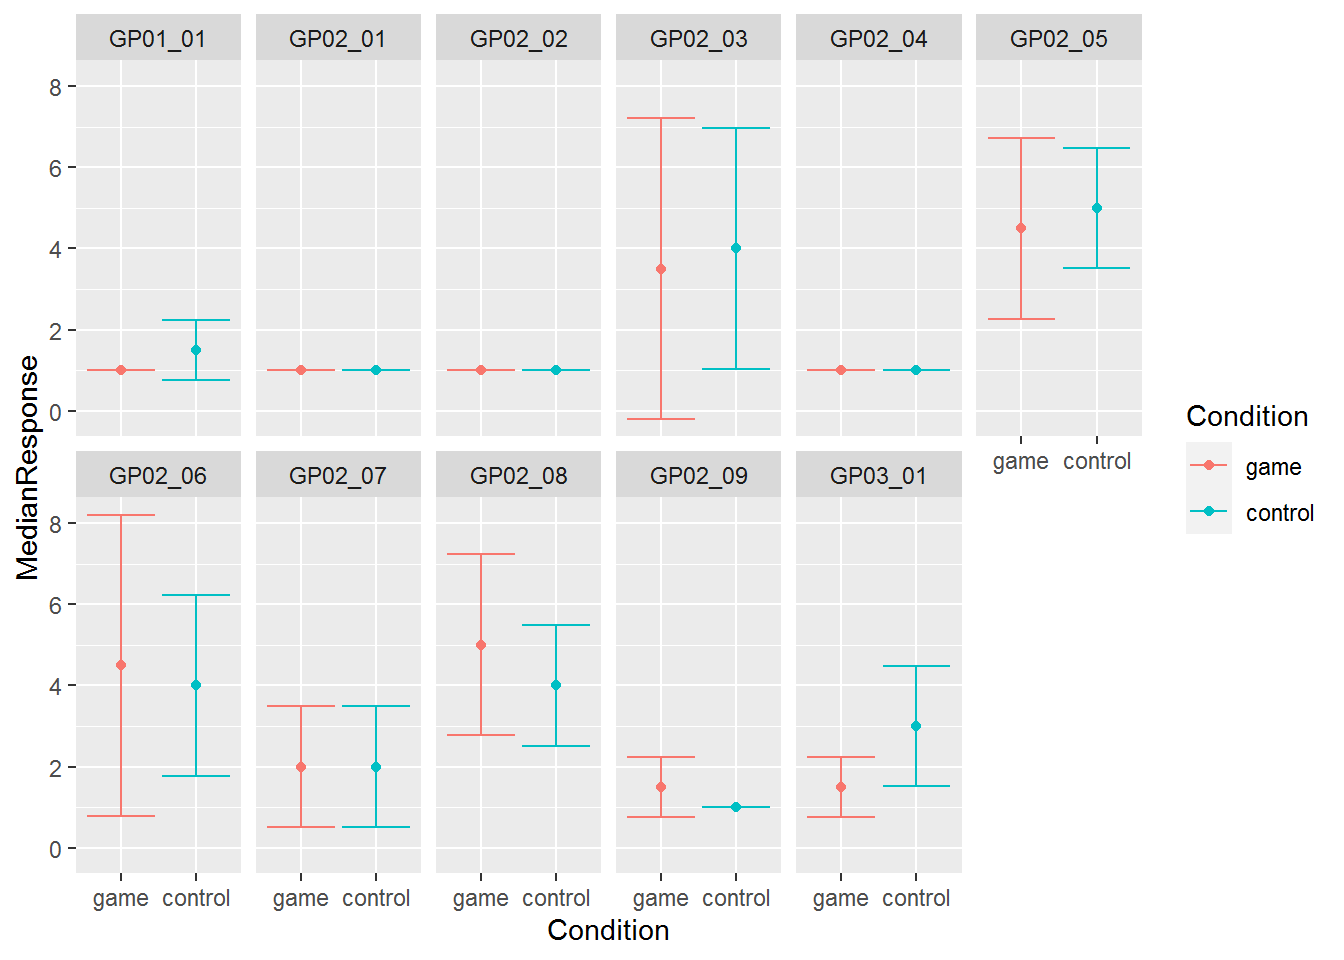
\includegraphics{data-analysis-using-r-for-psychology_files/figure-latex/unnamed-chunk-207-1} \end{center}

Do exercise 6.

Perform similar analysis but do not group data and summarize the data. Instead, use box plots to show the variability. Which visualization do you prefer?

\begin{center}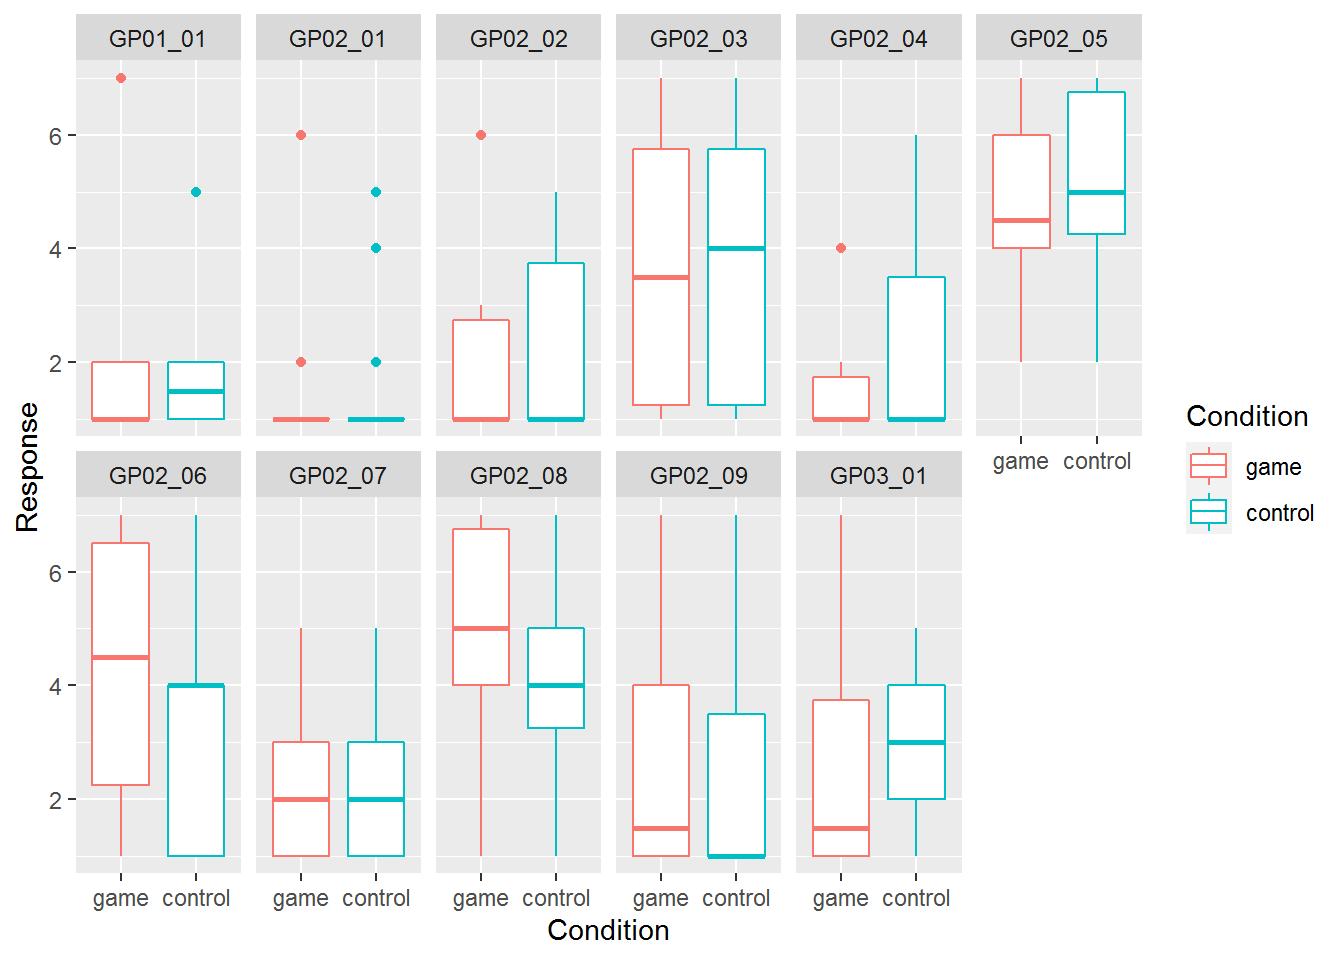
\includegraphics{data-analysis-using-r-for-psychology_files/figure-latex/unnamed-chunk-208-1} \end{center}

Do exercise 7.

\hypertarget{pivot-wider}{%
\section{Pivot wider}\label{pivot-wider}}

You can also always go from a long to a wide representation via \href{https://tidyr.tidyverse.org/reference/pivot_wider.html}{pivot\_wider()} or \href{https://stat.ethz.ch/R-manual/R-patched/library/stats/html/reshape.html}{reshape} functions. The logic is reverse, you need to specify which columns \emph{identify} different rows that belong together, which columns contain column names, and which contain their values. For our example table the names of the columns are in the column \texttt{Scale} and values are in \texttt{Response}. But what about columns that identify the rows that belong together? In our case, these are \texttt{Participant} and \texttt{Face}, so all rows from a \emph{long} table that have same combination of \texttt{Participant} and \texttt{Face} values should be merged together into a single row. If you do not explicitly specify \texttt{id\_cols}, then by default, \href{https://tidyr.tidyverse.org/reference/pivot_wider.html}{pivot\_wider()} will use \emph{all other remaining columns} to identify which rows belong together. This is irrelevant in this toy example, as \texttt{Participant} and \texttt{Face} is all we have left anyhow but below I will show you how things can get confusing and how to overcome this.

Let us undo our previous wide-to-long transformation and get our original wide table back!\footnote{I used table as an explicit first argument for \texttt{pivot\_longer()} but piped it to \texttt{pivot\_wider()}, why? To remind you that these two ways are the interchangeable and that both put the table as a parameter into the function.}

\begin{Shaded}
\begin{Highlighting}[]
\NormalTok{wide\_again\_tidy }\OtherTok{\textless{}{-}}
\NormalTok{  long\_tidy }\SpecialCharTok{\%\textgreater{}\%}
  \FunctionTok{pivot\_wider}\NormalTok{(}\AttributeTok{names\_from =} \StringTok{"Scale"}\NormalTok{, }\AttributeTok{values\_from=}\StringTok{"Response"}\NormalTok{)}
\end{Highlighting}
\end{Shaded}

Or, using explicit \texttt{id\_cols}

\begin{Shaded}
\begin{Highlighting}[]
\NormalTok{wide\_again\_tidy }\OtherTok{\textless{}{-}}
\NormalTok{  long\_tidy }\SpecialCharTok{\%\textgreater{}\%}
  \FunctionTok{pivot\_wider}\NormalTok{(}\AttributeTok{id\_cols =} \FunctionTok{c}\NormalTok{(}\StringTok{"Participant"}\NormalTok{, }\StringTok{"Face"}\NormalTok{), }\AttributeTok{names\_from =} \StringTok{"Scale"}\NormalTok{, }\AttributeTok{values\_from=}\StringTok{"Response"}\NormalTok{)}
\end{Highlighting}
\end{Shaded}

\begin{table}

\caption{\label{tab:unnamed-chunk-211}Our table is wide again!}
\centering
\begin{tabular}[t]{r|l|r|r|r}
\hline
Participant & Face & Symmetry & Attractiveness & Trustworthiness\\
\hline
1 & M-1 & 6 & 4 & 3\\
\hline
1 & M-2 & 4 & 7 & 6\\
\hline
2 & M-1 & 5 & 2 & 1\\
\hline
2 & M-2 & 3 & 7 & 2\\
\hline
\end{tabular}
\end{table}

You can pivot wider using \href{https://stat.ethz.ch/R-manual/R-patched/library/stats/html/reshape.html}{reshape()} as well. However, note that, as of 01.11.2021, it works correctly \emph{only} with data frames, so if you have a \href{https://tibble.tidyverse.org/}{tibble} (as I do), you need to convert it to a data frame via \href{https://stat.ethz.ch/R-manual/R-patched/library/base/html/data.frame.html}{data.frame()} or \href{https://stat.ethz.ch/R-manual/R-patched/library/base/html/as.data.frame.html}{as.data.frame()}. Otherwise, you need to specify

\begin{itemize}
\tightlist
\item
  \texttt{direction\ =\ "wide"}
\item
  \texttt{idvar} : different rows that belong together. Same as \texttt{id\_cols} for \href{https://tidyr.tidyverse.org/reference/pivot_wider.html}{pivot\_wider()} but no defaults here.
\item
  \texttt{timevar} : same as \texttt{names\_from} for \href{https://tidyr.tidyverse.org/reference/pivot_wider.html}{pivot\_wider()}, column with values that will be used as column names.
\item
  \texttt{v.names} : same as \texttt{values\_from}.
\item
  \texttt{sep}: the new column names will constructed as \texttt{v.names} + \texttt{sep} + \texttt{timevar}. By default \texttt{sep="."}.
\end{itemize}

The main difference, as compared to \href{https://tidyr.tidyverse.org/reference/pivot_wider.html}{pivot\_wider()}, is how the column names are constructed. With \href{https://stat.ethz.ch/R-manual/R-patched/library/stats/html/reshape.html}{reshape()} function, the \texttt{v.names} + \texttt{sep} + \texttt{timevar} rule means that you end up with column names such as \texttt{Response.Symmetry} instead of just \texttt{Symmetry}.

\begin{Shaded}
\begin{Highlighting}[]
\NormalTok{wide\_again\_base }\OtherTok{\textless{}{-}} \FunctionTok{reshape}\NormalTok{(}\FunctionTok{as.data.frame}\NormalTok{(long\_tidy),}
                           \AttributeTok{direction =} \StringTok{"wide"}\NormalTok{,}
                           \AttributeTok{idvar =} \FunctionTok{c}\NormalTok{(}\StringTok{"Participant"}\NormalTok{, }\StringTok{"Face"}\NormalTok{),}
                           \AttributeTok{timevar =} \StringTok{"Scale"}\NormalTok{,}
                           \AttributeTok{v.names =} \StringTok{"Response"}\NormalTok{,}
                           \AttributeTok{sep =} \StringTok{"\_"}\NormalTok{)}
\end{Highlighting}
\end{Shaded}

Let us take a look at the importance of \texttt{id\_cols}. Imagine that we have \emph{another} column, say, response times. So, our long table will look like this

\begin{Shaded}
\begin{Highlighting}[]
\NormalTok{long\_tidy\_rt }\OtherTok{\textless{}{-}}
\NormalTok{  long\_tidy }\SpecialCharTok{\%\textgreater{}\%}
  \FunctionTok{ungroup}\NormalTok{() }\SpecialCharTok{\%\textgreater{}\%}
  \FunctionTok{mutate}\NormalTok{(}\AttributeTok{RT =} \FunctionTok{round}\NormalTok{(}\FunctionTok{rgamma}\NormalTok{(}\FunctionTok{n}\NormalTok{(), }\DecValTok{4}\NormalTok{, }\DecValTok{3}\NormalTok{), }\DecValTok{2}\NormalTok{))}
\end{Highlighting}
\end{Shaded}

\begin{tabular}{r|l|l|r|r}
\hline
Participant & Face & Scale & Response & RT\\
\hline
1 & M-1 & Symmetry & 6 & 1.48\\
\hline
1 & M-1 & Attractiveness & 4 & 1.55\\
\hline
1 & M-1 & Trustworthiness & 3 & 1.18\\
\hline
1 & M-2 & Symmetry & 4 & 2.47\\
\hline
1 & M-2 & Attractiveness & 7 & 0.66\\
\hline
1 & M-2 & Trustworthiness & 6 & 1.30\\
\hline
2 & M-1 & Symmetry & 5 & 1.58\\
\hline
2 & M-1 & Attractiveness & 2 & 0.63\\
\hline
2 & M-1 & Trustworthiness & 1 & 1.12\\
\hline
2 & M-2 & Symmetry & 3 & 1.56\\
\hline
2 & M-2 & Attractiveness & 7 & 1.60\\
\hline
2 & M-2 & Trustworthiness & 2 & 0.51\\
\hline
\end{tabular}

For \href{https://tidyr.tidyverse.org/reference/pivot_wider.html}{pivot\_wider}, if we do not specify which columns identify rows that belong together, \texttt{RT} will be used as well. But, because it is different for every response, each row in the original table will be unique and we will end up with a weird looking table wit lots of \texttt{NAs}.

\begin{Shaded}
\begin{Highlighting}[]
\NormalTok{wide\_odd\_rt }\OtherTok{\textless{}{-}}
  \FunctionTok{pivot\_wider}\NormalTok{(long\_tidy\_rt, }\AttributeTok{names\_from =} \StringTok{"Scale"}\NormalTok{, }\AttributeTok{values\_from=}\StringTok{"Response"}\NormalTok{)}
\end{Highlighting}
\end{Shaded}

\begin{tabular}{r|l|r|r|r|r}
\hline
Participant & Face & RT & Symmetry & Attractiveness & Trustworthiness\\
\hline
1 & M-1 & 1.48 & 6 & NA & NA\\
\hline
1 & M-1 & 1.55 & NA & 4 & NA\\
\hline
1 & M-1 & 1.18 & NA & NA & 3\\
\hline
1 & M-2 & 2.47 & 4 & NA & NA\\
\hline
1 & M-2 & 0.66 & NA & 7 & NA\\
\hline
1 & M-2 & 1.30 & NA & NA & 6\\
\hline
2 & M-1 & 1.58 & 5 & NA & NA\\
\hline
2 & M-1 & 0.63 & NA & 2 & NA\\
\hline
2 & M-1 & 1.12 & NA & NA & 1\\
\hline
2 & M-2 & 1.56 & 3 & NA & NA\\
\hline
2 & M-2 & 1.60 & NA & 7 & NA\\
\hline
2 & M-2 & 0.51 & NA & NA & 2\\
\hline
\end{tabular}

To remedy that, we need to specify id columns explicitly, so that \texttt{pivot\_wider()} can ignore and \emph{drop} the rest:

\begin{Shaded}
\begin{Highlighting}[]
\NormalTok{wide\_rt }\OtherTok{\textless{}{-}}
  \FunctionTok{pivot\_wider}\NormalTok{(long\_tidy\_rt,}
              \AttributeTok{id\_cols =} \FunctionTok{c}\NormalTok{(}\StringTok{"Participant"}\NormalTok{, }\StringTok{"Face"}\NormalTok{),}
              \AttributeTok{names\_from =} \StringTok{"Scale"}\NormalTok{,}
              \AttributeTok{values\_from=}\StringTok{"Response"}\NormalTok{) }
\end{Highlighting}
\end{Shaded}

\begin{tabular}{r|l|r|r|r}
\hline
Participant & Face & Symmetry & Attractiveness & Trustworthiness\\
\hline
1 & M-1 & 6 & 4 & 3\\
\hline
1 & M-2 & 4 & 7 & 6\\
\hline
2 & M-1 & 5 & 2 & 1\\
\hline
2 & M-2 & 3 & 7 & 2\\
\hline
\end{tabular}

For practice, let us take \href{data/bands-adaptation.csv}{adaptation} data and turn it onto a wide format that is easier for humans to read. In the original form, the table is a long format with a row for each pair of prime and probe stimuli.

\begin{tabular}{l|l|l|r|r}
\hline
Participant & Prime & Probe & Nsame & Ntotal\\
\hline
ma2 & Sphere & Sphere & 22 & 119\\
\hline
ma2 & Sphere & Quadro & 23 & 118\\
\hline
ma2 & Sphere & Dual & 15 & 120\\
\hline
ma2 & Sphere & Single & 31 & 115\\
\hline
\end{tabular}

Let us turn it into a wider table, so that a single row corresponds to a single prime and four new column contain proportion of same responses for individual probes. The table will look like this (use \href{https://stat.ethz.ch/R-manual/R-devel/library/base/html/Round.html}{round()} function to reduce the number of digits):

\begin{tabular}{l|l|r|r|r|r|r}
\hline
Participant & Prime & Sphere & Quadro & Dual & Single & Average\\
\hline
ma2 & Sphere & 0.18 & 0.19 & 0.12 & 0.27 & 0.1900\\
\hline
ma2 & Quadro & 0.21 & 0.22 & 0.14 & 0.34 & 0.2275\\
\hline
ma2 & Dual & 0.25 & 0.30 & 0.27 & 0.48 & 0.3250\\
\hline
ma2 & Single & 0.34 & 0.30 & 0.48 & 0.39 & 0.3775\\
\hline
\end{tabular}

The overall procedure is fairly straightforward:

\begin{enumerate}
\def\labelenumi{\arabic{enumi}.}
\tightlist
\item
  Read the file (don't forget to specify column types)
\item
  Computer \texttt{Psame} proportion of same responses given number of total responses for each .
\item
  Pivot the table wider, think about your id columns. Also try this without specifying any and see what you get.
\item
  Compute an average stability across all probes and put it into a new \texttt{Average} column. You can do it ``by hand'' but, instead, use \href{https://stat.ethz.ch/R-manual/R-devel/library/base/html/colSums.html}{rowSums()} to compute it. Here, use \texttt{.} to refer to the table inside the \texttt{mutate()} function and you will need to normalize it by the number of probes to get an average instead of the sum.
\item
  Pipe it to the output, using \href{https://bookdown.org/yihui/rmarkdown-cookbook/kable.html}{knitr::kable()}.
\end{enumerate}

Use \href{https://tidyr.tidyverse.org/reference/pivot_wider.html}{pivot\_wider()} in exercise 8.\\
::: \{.infobox .practice\}
Do exercise 8.
:::

Repeat the analysis but now using the \href{https://stat.ethz.ch/R-manual/R-patched/library/stats/html/reshape.html}{reshape()} function.
::: \{.infobox .practice\}
Do exercise 9.
:::

Let us practice more and create group average summary as a square 5×4 table with a single row per \emph{Prime} and four columns for \emph{Probe} plus a column that says which prime the row corresponds to. As a value for each cell, we want to code a \_median value. The table should look like this:

\begin{tabular}{c|c|c|c|c}
\hline
Prime & Sphere & Quadro & Dual & Single\\
\hline
Sphere & 0.13 & 0.13 & 0.17 & 0.32\\
\hline
Quadro & 0.19 & 0.12 & 0.21 & 0.38\\
\hline
Dual & 0.15 & 0.30 & 0.27 & 0.48\\
\hline
Single & 0.34 & 0.30 & 0.48 & 0.51\\
\hline
\end{tabular}

You know almost everything you need, so think about how you would implement this as a \emph{single} pipeline. Hints: to match my table you will definitely to convert \texttt{Prime} and \texttt{Probe} to factors to ensure consistent ordering (otherwise, they will be sorted alphabetically), you will need to \href{https://dplyr.tidyverse.org/reference/group_by.html}{group} individual combinations of prime and probe before computing a \href{https://dplyr.tidyverse.org/reference/summarise.html}{summary statistics}. And, of course, you will need to pivot the table wider (use your preferred method).

Do exercise 10.

\hypertarget{controling-computation-flow}{%
\chapter{Controling computation flow}\label{controling-computation-flow}}

Grab the \href{notebooks/Seminar\%2010\%20-\%20repetition.Rmd}{exercise notebook} before we start.

One the most powerful features of R is that it is vector-based. Remember, everything is a vector (or a list). In the previous seminars you saw you can apply a function, a filter, or perform a computation on all values of a vector or all rows in a table in a single call. However, sometimes, you need to go over one value or row at a time explicitly. For example, if you working with a time-series, it might be easier to use an explicit \href{https://stat.ethz.ch/R-manual/R-devel/library/base/html/Control.html}{for} loop to compute current value based on previous state of the system. However, such instances are fairly rare, so the general rule for R is ``you probably do not need a loop''. Below, we will go through various tools that render explicit loops redundant.

\hypertarget{rep}{%
\section{\texorpdfstring{\texttt{rep()}}{rep()}}\label{rep}}

The most basic repetition mechanism in R is \href{https://stat.ethz.ch/R-manual/R-devel/library/base/html/rep.html}{rep()} function. It takes a vector and repeats it specified number of \emph{times}.

\begin{Shaded}
\begin{Highlighting}[]
\FunctionTok{rep}\NormalTok{(}\FunctionTok{c}\NormalTok{(}\DecValTok{1}\NormalTok{, }\DecValTok{2}\NormalTok{, }\DecValTok{3}\NormalTok{), }\AttributeTok{times=}\DecValTok{4}\NormalTok{)}
\end{Highlighting}
\end{Shaded}

\begin{verbatim}
##  [1] 1 2 3 1 2 3 1 2 3 1 2 3
\end{verbatim}

Alternatively, you can repeat each element specified number of times before repeating the next one via \texttt{each} parameter. The difference between options lies only in the \emph{order} of elements in the new vector. As you can see both vectors have the same length and each individual value is repeated four times.

\begin{Shaded}
\begin{Highlighting}[]
\FunctionTok{rep}\NormalTok{(}\FunctionTok{c}\NormalTok{(}\DecValTok{1}\NormalTok{, }\DecValTok{2}\NormalTok{, }\DecValTok{3}\NormalTok{), }\AttributeTok{each=}\DecValTok{4}\NormalTok{)}
\end{Highlighting}
\end{Shaded}

\begin{verbatim}
##  [1] 1 1 1 1 2 2 2 2 3 3 3 3
\end{verbatim}

You can specify length of the output vector via \texttt{length.out}. When combined with \texttt{times} it can be useful for producing truncated vectors. E.g., when we repeat a three element vector but we want to get ten values. Using \texttt{times} only, we can get either nine (\texttt{times=3}) or twelve (\texttt{times=4}), not ten. \texttt{length.out=10} makes it happen.

\begin{Shaded}
\begin{Highlighting}[]
\FunctionTok{rep}\NormalTok{(}\FunctionTok{c}\NormalTok{(}\DecValTok{1}\NormalTok{, }\DecValTok{2}\NormalTok{, }\DecValTok{3}\NormalTok{), }\AttributeTok{times=}\DecValTok{4}\NormalTok{, }\AttributeTok{length.out =} \DecValTok{10}\NormalTok{)}
\end{Highlighting}
\end{Shaded}

\begin{verbatim}
##  [1] 1 2 3 1 2 3 1 2 3 1
\end{verbatim}

However, you can also use subsetting of a new vector to achieve the same end.

\begin{Shaded}
\begin{Highlighting}[]
\FunctionTok{rep}\NormalTok{(}\FunctionTok{c}\NormalTok{(}\DecValTok{1}\NormalTok{, }\DecValTok{2}\NormalTok{, }\DecValTok{3}\NormalTok{), }\AttributeTok{times=}\DecValTok{4}\NormalTok{)[}\DecValTok{1}\SpecialCharTok{:}\DecValTok{10}\NormalTok{]}
\end{Highlighting}
\end{Shaded}

\begin{verbatim}
##  [1] 1 2 3 1 2 3 1 2 3 1
\end{verbatim}

You should be more careful when combining \texttt{length.out} with \texttt{each}, as each value is repeated \texttt{each} times and, if \texttt{length.out} is longer, the same sequence is repeated again. Could be confusing and you might get a very unbalanced repeated sequence.

\begin{Shaded}
\begin{Highlighting}[]
\FunctionTok{rep}\NormalTok{(}\FunctionTok{c}\NormalTok{(}\DecValTok{1}\NormalTok{, }\DecValTok{2}\NormalTok{, }\DecValTok{3}\NormalTok{), }\AttributeTok{each=}\DecValTok{8}\NormalTok{, }\AttributeTok{length.out =} \DecValTok{10}\NormalTok{)}
\end{Highlighting}
\end{Shaded}

\begin{verbatim}
##  [1] 1 1 1 1 1 1 1 1 2 2
\end{verbatim}

Do exercise 1.

\hypertarget{repeating-combinations}{%
\section{Repeating combinations}\label{repeating-combinations}}

To create a table with all combinations of values, you can use either base R \href{https://stat.ethz.ch/R-manual/R-devel/library/base/html/expand.grid.html}{expand.grid()} or tidyr's implementation \href{https://tidyr.tidyverse.org/reference/expand_grid.html}{expand\_grid()}. The latter is a bit more robust and can expand even tables and matrices (but see the documentation for subtle differences in implementation and output).

The usage is very straightforward, you provide column names and values and you get all combinations of their values.

\begin{Shaded}
\begin{Highlighting}[]
\NormalTok{knitr}\SpecialCharTok{::}\FunctionTok{kable}\NormalTok{(grid\_base)}
\end{Highlighting}
\end{Shaded}

\begin{tabular}{l|l|l}
\hline
gender & handidness & colorblindness\\
\hline
female & right & TRUE\\
\hline
male & right & TRUE\\
\hline
female & left & TRUE\\
\hline
male & left & TRUE\\
\hline
female & right & FALSE\\
\hline
male & right & FALSE\\
\hline
female & left & FALSE\\
\hline
male & left & FALSE\\
\hline
\end{tabular}

\href{https://tidyr.tidyverse.org/reference/expand_grid.html}{expand\_grid()} works the same they but for the order in the values very within columns.

\begin{Shaded}
\begin{Highlighting}[]
\FunctionTok{expand\_grid}\NormalTok{(}\AttributeTok{gender=}\FunctionTok{c}\NormalTok{(}\StringTok{"female"}\NormalTok{, }\StringTok{"male"}\NormalTok{), }
            \AttributeTok{handidness=}\FunctionTok{c}\NormalTok{(}\StringTok{"right"}\NormalTok{, }\StringTok{"left"}\NormalTok{),}
            \AttributeTok{colorblindness=}\FunctionTok{c}\NormalTok{(}\ConstantTok{TRUE}\NormalTok{, }\ConstantTok{FALSE}\NormalTok{))}
\end{Highlighting}
\end{Shaded}

\begin{Shaded}
\begin{Highlighting}[]
\NormalTok{knitr}\SpecialCharTok{::}\FunctionTok{kable}\NormalTok{(grid\_tidyr)}
\end{Highlighting}
\end{Shaded}

\begin{tabular}{l|l|l}
\hline
gender & handidness & colorblindness\\
\hline
female & right & TRUE\\
\hline
female & right & FALSE\\
\hline
female & left & TRUE\\
\hline
female & left & FALSE\\
\hline
male & right & TRUE\\
\hline
male & right & FALSE\\
\hline
male & left & TRUE\\
\hline
male & left & FALSE\\
\hline
\end{tabular}

Do exercise 2.

\hypertarget{forloop}{%
\section{For loop}\label{forloop}}

You can loop (iterate) over elements of a vector or list via a \href{https://stat.ethz.ch/R-manual/R-devel/library/base/html/Control.html}{for} loop, which is very similar to for-loops in other programming languages. However, use of the \texttt{for} loop in R is fairly rare, because vectors are a fundamental building block of R and, therefore, it is inherently vectorized (you can do the same thing to all values, not to one value at a time). Thus, almost always, you can do the same thing but using simpler or more expressive tools. In a sense, \texttt{for} loop is very un-R, so if you find yourself using it, consider whether there is a simpler or more expressive way to do this. At the same time, if \texttt{for} loop \emph{is} the simplest or clearest way to write you code, by all means, use it!

The general format is

\begin{Shaded}
\begin{Highlighting}[]
\ControlFlowTok{for}\NormalTok{(loop\_variable }\ControlFlowTok{in}\NormalTok{ vector\_or\_list)\{}
\NormalTok{  ...some operations using loop\_variable that}
\NormalTok{  changes its value on each iteration... }
\NormalTok{\}}
\end{Highlighting}
\end{Shaded}

Note the curly brackets. We used them before to put the code inside a function. Here, we use them to put the code inside the loop. The loop is repeated as many times as the number of elements in a vector or a list with a loop variable\footnote{Just a reminder, the loop variable can have \emph{any} name. Often, you see people using \texttt{i} but I would strongly recommend going for a more meaningful name.} getting assigned each vector/list value on each iteration. Thus, to print each value of a vector we can do

\begin{Shaded}
\begin{Highlighting}[]
\ControlFlowTok{for}\NormalTok{(a\_number }\ControlFlowTok{in} \FunctionTok{c}\NormalTok{(}\DecValTok{1}\NormalTok{, }\DecValTok{5}\NormalTok{, }\DecValTok{200}\NormalTok{))\{}
  \FunctionTok{print}\NormalTok{(a\_number)}
\NormalTok{\}}
\end{Highlighting}
\end{Shaded}

\begin{verbatim}
## [1] 1
## [1] 5
## [1] 200
\end{verbatim}

A typical scenario is for the loop variable to be an \emph{index} that can be used to access element of a vector or a list. You can build a vector of indexes via \texttt{start:stop} sequence tool we used for \protect\hyperlink{vector-index-slicing}{slicing}. You can compute a length of an object via \href{https://stat.ethz.ch/R-manual/R-devel/library/base/html/length.html}{length()} function. For a \texttt{data.frame} or a \texttt{tibble}, you can figure out number of rows and columns via, respectively, \href{https://stat.ethz.ch/R-manual/R-devel/library/base/html/nrow.html}{nrow()} and \href{https://stat.ethz.ch/R-manual/R-devel/library/base/html/nrow.html}{ncol()} functions.

\begin{Shaded}
\begin{Highlighting}[]
\NormalTok{vector\_of\_some\_numbers }\OtherTok{\textless{}{-}} \FunctionTok{c}\NormalTok{(}\DecValTok{1}\NormalTok{, }\DecValTok{5}\NormalTok{, }\DecValTok{200}\NormalTok{)}
\ControlFlowTok{for}\NormalTok{(index }\ControlFlowTok{in} \DecValTok{1}\SpecialCharTok{:}\FunctionTok{length}\NormalTok{(vector\_of\_some\_numbers))\{}
  \FunctionTok{print}\NormalTok{(vector\_of\_some\_numbers[index])}
\NormalTok{\}}
\end{Highlighting}
\end{Shaded}

\begin{verbatim}
## [1] 1
## [1] 5
## [1] 200
\end{verbatim}

Do exercise 3.

You can also \emph{nest} loops (wondering what \href{https://stat.ethz.ch/R-manual/R-devel/library/base/html/cat.html}{cat()} does? Concatenates and ptings, so read the \href{https://stat.ethz.ch/R-manual/R-devel/library/base/html/cat.html}{manual}!).

\begin{Shaded}
\begin{Highlighting}[]
\ControlFlowTok{for}\NormalTok{(letter }\ControlFlowTok{in} \FunctionTok{c}\NormalTok{(}\StringTok{"A"}\NormalTok{, }\StringTok{"B"}\NormalTok{, }\StringTok{"C"}\NormalTok{))\{}
  \ControlFlowTok{for}\NormalTok{(number }\ControlFlowTok{in} \DecValTok{1}\SpecialCharTok{:}\DecValTok{2}\NormalTok{)\{}
    \FunctionTok{cat}\NormalTok{(letter, number, }\StringTok{"}\SpecialCharTok{\textbackslash{}n}\StringTok{"}\NormalTok{)}
\NormalTok{  \}}
\NormalTok{\}}
\end{Highlighting}
\end{Shaded}

\begin{verbatim}
## A 1 
## A 2 
## B 1 
## B 2 
## C 1 
## C 2
\end{verbatim}

Do exercise 4.

As I have noted above, loops are particularly useful when you current value depends on a previous one (or many previous values). In the next exercise, use \texttt{for} loop to create a random walk with an initial value of zero. For each next step, draw a random value from a normal distribution with zero mean and standard deviation computed as \texttt{exp(value\_on\_previous\_step)} (the function you are looking for is \href{https://stat.ethz.ch/R-manual/R-devel/library/stats/html/Normal.html}{rnorm()}). Generate a ten-step, that might look like this

\begin{verbatim}
##  [1]  0.00000000 -0.56902925 -0.23326972  0.04788655 -0.26527382  0.05453601
##  [7]  0.21423641 -1.36139599 -0.27036963  0.76728873
\end{verbatim}

Do exercise 5.

\hypertarget{conditional-statement}{%
\section{Conditional statement}\label{conditional-statement}}

As for all other programming languages, you can control the flow of execution using \href{https://stat.ethz.ch/R-manual/R-devel/library/base/html/Control.html}{if-else} statements. The general usage is as follows.

\begin{Shaded}
\begin{Highlighting}[]
\ControlFlowTok{if}\NormalTok{ (some\_condition) \{}
  \CommentTok{\# code runs if some\_condition is TRUE}
\NormalTok{\} }\ControlFlowTok{else}\NormalTok{ \{}
  \CommentTok{\# code runs if some\_condition is FALSE}
\NormalTok{\}}
\end{Highlighting}
\end{Shaded}

For example, we can define our condition using \href{https://stat.ethz.ch/R-manual/R-devel/library/base/html/Comparison.html}{mathematical comparisons}.

\begin{Shaded}
\begin{Highlighting}[]
\NormalTok{x }\OtherTok{\textless{}{-}} \SpecialCharTok{{-}}\DecValTok{3}
\ControlFlowTok{if}\NormalTok{ (x }\SpecialCharTok{\textgreater{}} \DecValTok{0}\NormalTok{) \{}
  \FunctionTok{cat}\NormalTok{(}\StringTok{"X is definitely greater than  zero"}\NormalTok{)}
\NormalTok{\} }\ControlFlowTok{else}\NormalTok{ \{}
  \FunctionTok{cat}\NormalTok{(}\StringTok{"X is not greater than zero."}\NormalTok{)}
\NormalTok{\}}
\end{Highlighting}
\end{Shaded}

\begin{verbatim}
## X is not greater than zero.
\end{verbatim}

You can combine several conditions using \href{https://stat.ethz.ch/R-manual/R-devel/library/base/html/Logic.html}{logical operators} such as \emph{and} \texttt{\&} or \emph{or} \texttt{\textbar{}}. For example, we can check whether x is smaller than zero but larger than -10.

\begin{Shaded}
\begin{Highlighting}[]
\NormalTok{x }\OtherTok{\textless{}{-}} \SpecialCharTok{{-}}\DecValTok{3}
\ControlFlowTok{if}\NormalTok{ ((x }\SpecialCharTok{\textless{}} \DecValTok{0}\NormalTok{) }\SpecialCharTok{\&}\NormalTok{ (x }\SpecialCharTok{\textgreater{}} \SpecialCharTok{{-}}\DecValTok{10}\NormalTok{)) \{}
  \FunctionTok{cat}\NormalTok{(}\StringTok{"Bingo!"}\NormalTok{)}
\NormalTok{\} }\ControlFlowTok{else}\NormalTok{ \{}
  \FunctionTok{cat}\NormalTok{(}\StringTok{"I don\textquotesingle{}t like this x."}\NormalTok{)}
\NormalTok{\}}
\end{Highlighting}
\end{Shaded}

\begin{verbatim}
## Bingo!
\end{verbatim}

Beware that the \href{https://stat.ethz.ch/R-manual/R-devel/library/base/html/Control.html}{if} requires a \emph{single} logical value to work. If you have more than one value, it will use \emph{only the first one} but it will give you a warning.

\begin{Shaded}
\begin{Highlighting}[]
\NormalTok{x }\OtherTok{\textless{}{-}} \FunctionTok{c}\NormalTok{(}\DecValTok{10}\NormalTok{,  }\SpecialCharTok{{-}}\DecValTok{3}\NormalTok{)}
\ControlFlowTok{if}\NormalTok{ ((x }\SpecialCharTok{\textless{}} \DecValTok{0}\NormalTok{)) \{}
  \FunctionTok{cat}\NormalTok{(}\StringTok{"Bingo!"}\NormalTok{)}
\NormalTok{\} }\ControlFlowTok{else}\NormalTok{ \{}
  \FunctionTok{cat}\NormalTok{(}\StringTok{"I don\textquotesingle{}t like this x."}\NormalTok{)}
\NormalTok{\}}
\end{Highlighting}
\end{Shaded}

\begin{verbatim}
## Warning in if ((x < 0)) {: the condition has length > 1 and only the first
## element will be used
\end{verbatim}

\begin{verbatim}
## I don't like this x.
\end{verbatim}

Also beware that R has both \texttt{\&}/\texttt{\textbar{}} and \texttt{\&\&}/\texttt{\textbar{}\textbar{}} versions of \emph{and} and \emph{or} logical operators (single versus double the number of symbols). Both perform logical operations on vectors but double-symbol ones return only the \emph{first} value. E.g., single-symbol returns \texttt{TRUE}/\texttt{FALSE} for each value of \texttt{x}

\begin{Shaded}
\begin{Highlighting}[]
\NormalTok{x }\OtherTok{\textless{}{-}} \FunctionTok{c}\NormalTok{(}\DecValTok{10}\NormalTok{, }\SpecialCharTok{{-}}\DecValTok{3}\NormalTok{, }\SpecialCharTok{{-}}\DecValTok{11}\NormalTok{)}
\NormalTok{(x }\SpecialCharTok{\textless{}} \DecValTok{0}\NormalTok{) }\SpecialCharTok{\&}\NormalTok{ (x }\SpecialCharTok{\textgreater{}} \SpecialCharTok{{-}}\DecValTok{10}\NormalTok{)}
\end{Highlighting}
\end{Shaded}

\begin{verbatim}
## [1] FALSE  TRUE FALSE
\end{verbatim}

But double-symbol returns it only for the \emph{first} value.

\begin{Shaded}
\begin{Highlighting}[]
\NormalTok{(x }\SpecialCharTok{\textless{}} \DecValTok{0}\NormalTok{) }\SpecialCharTok{\&\&}\NormalTok{ (x }\SpecialCharTok{\textgreater{}} \SpecialCharTok{{-}}\DecValTok{10}\NormalTok{)}
\end{Highlighting}
\end{Shaded}

\begin{verbatim}
## [1] FALSE
\end{verbatim}

I am sure there is a perfectly logical explanation for this bizarre implementation but I do not know it. I am bringing this up, just so that you would \emph{never} use double-symbol logical operators! Chances are, you will forget about this ``return-only-the-first-value'' behavior and expect them to act normally. They won't behave as you think they should, so simply stay away.

Let us combine \texttt{for} loop with \texttt{if-else} operator. Generate a vector of ten normally distributed values (again, \href{https://stat.ethz.ch/R-manual/R-devel/library/stats/html/Normal.html}{rnorm()} is the function). Loop over them in a \texttt{for} loop and \href{https://stat.ethz.ch/R-manual/R-devel/library/base/html/print.html}{print()} \texttt{"Positive"} if a value is larger than zero and \texttt{"Not\ positive"} if not. The results should look like this\footnote{Want exact same numbers as I do? Use \texttt{set.seed(164)}. This function, see \href{https://stat.ethz.ch/R-manual/R-devel/library/base/html/Random.html}{set.seed()} makes random generators start at a specific point, so that the you will get the \emph{same} sequence of \emph{random} numbers as I did.}

\begin{verbatim}
##  [1]  0.03003683  1.22390943  1.71573769 -0.89994016  0.55507190  0.42319195
##  [7]  0.82993426 -1.28614375  1.21511589 -0.05815403
\end{verbatim}

\begin{verbatim}
## [1] "Positive"
## [1] "Positive"
## [1] "Positive"
## [1] "Not positive"
## [1] "Positive"
## [1] "Positive"
## [1] "Positive"
## [1] "Not positive"
## [1] "Positive"
## [1] "Not positive"
\end{verbatim}

Do exercise 6. (NOT YET IMPLEMENTED!)

\hypertarget{breaking-out-of-the-loop}{%
\section{Breaking out of the loop}\label{breaking-out-of-the-loop}}

The code inside the \href{https://stat.ethz.ch/R-manual/R-devel/library/base/html/Control.html}{for} loop is typically repeated for every value of the vector that you have supplied. However, there is a way to \href{https://stat.ethz.ch/R-manual/R-devel/library/base/html/Control.html}{break} out of it using a \texttt{break} statement. This stops execution of the code \emph{inside} of the loop immediately and continues with the code immediately after the loop.

\begin{Shaded}
\begin{Highlighting}[]
\ControlFlowTok{for}\NormalTok{(y }\ControlFlowTok{in} \FunctionTok{c}\NormalTok{(}\DecValTok{1}\NormalTok{, }\DecValTok{2}\NormalTok{, }\DecValTok{3}\NormalTok{))\{}
  \FunctionTok{print}\NormalTok{(}\StringTok{"This will be exected"}\NormalTok{)}
  \ControlFlowTok{break}
  \FunctionTok{print}\NormalTok{(}\StringTok{"But this won\textquotesingle{}t be"}\NormalTok{)}
\NormalTok{\}}
\end{Highlighting}
\end{Shaded}

\begin{verbatim}
## [1] "This will be exected"
\end{verbatim}

\begin{Shaded}
\begin{Highlighting}[]
\FunctionTok{print}\NormalTok{(}\StringTok{"Now to the code AFTER the loop"}\NormalTok{)}
\end{Highlighting}
\end{Shaded}

\begin{verbatim}
## [1] "Now to the code AFTER the loop"
\end{verbatim}

Note that in this case, the code was executed (incompletely!) only once. Typically, \texttt{break} is used in combination with the \texttt{if-else} statement to break out of the loop, if a certain condition is met. Let us practice. Again, generate ten normally distributed numbers, loop over them and print each one. However, \texttt{break} after the \emph{fifth} value. For this, you need to loop over indexes of values (that go from 1 to the \href{https://stat.ethz.ch/R-manual/R-devel/library/base/html/length.html}{length()} of your vector). Thus, you loop variable will contain an index of each element of x (because of that I called it \texttt{ix}) and you need to use it to get a value at this position within the vector. If that index is equal to 5, break out of the loop.
For the ten values I've generated above, the output will be the following (``Done for today'' is printed after the loop).

\begin{Shaded}
\begin{Highlighting}[]
\FunctionTok{set.seed}\NormalTok{(}\DecValTok{164}\NormalTok{)}
\NormalTok{x }\OtherTok{\textless{}{-}} \FunctionTok{rnorm}\NormalTok{(}\DecValTok{10}\NormalTok{)}
\ControlFlowTok{for}\NormalTok{(ix }\ControlFlowTok{in} \DecValTok{1}\SpecialCharTok{:}\FunctionTok{length}\NormalTok{(x))\{}
  \ControlFlowTok{if}\NormalTok{ (ix }\SpecialCharTok{==} \DecValTok{5}\NormalTok{)  }\ControlFlowTok{break}
  \FunctionTok{print}\NormalTok{(x[ix])}
\NormalTok{\}}
\end{Highlighting}
\end{Shaded}

\begin{verbatim}
## [1] 0.03003683
## [1] 1.223909
## [1] 1.715738
## [1] -0.8999402
\end{verbatim}

\begin{Shaded}
\begin{Highlighting}[]
\FunctionTok{print}\NormalTok{(}\StringTok{"Done for today"}\NormalTok{)}
\end{Highlighting}
\end{Shaded}

\begin{verbatim}
## [1] "Done for today"
\end{verbatim}

Do exercise 7. (NOT YET IMPLEMENTED!)

\hypertarget{using-for-loop-to-load-and-join-multiple-data-files}{%
\section{Using for loop to load and join multiple data files}\label{using-for-loop-to-load-and-join-multiple-data-files}}

Your analysis starts with loading the data. Quite often, data for individual participants is stored in different files but with identical structure, so you need code that figures out which files you need to load, loads them on at a time and then binds them to one final table. Using a \texttt{for} loop is not the most elegant way to implement this but it does the job and gives you another example of how loops can be useful. I will walk you through details and then you We will implement the code that loads and merges individual files for persistence study. Download the \href{data/persistence.zip}{persistence.zip} and unzip into \texttt{Persistence} subfolder (we do not want to create a mess in your main folder!).

First, you need to have a character vector with relevant file names. Package you are looking for is \href{https://github.com/r-lib/fs}{fs} (for \textbf{f}ile \textbf{s}ystem). It has everything you need to work with the file system, including working with file names (dropping or adding path, extension, etc.), creating/moving/deleting files, checking whether file exists, and what not. One function that I use the most is \href{https://www.rdocumentation.org/packages/fs/versions/1.5.0/topics/dir_ls}{dir\_ls()} that list files in a specified folder. The two parameters you need are \texttt{path} to your folder (you can use relative path) and, optionally, \texttt{glob} filter string. The latter is a \href{https://en.wikipedia.org/wiki/Glob_(programming)}{globbing} wildcard pattern, where \texttt{*} stands for ``any sequence of characters'' and \texttt{?} stand for "one arbitrary character. For a csv file, this pattern would be \texttt{"*.csv"}. Test this single function call using appropriate \texttt{path} and \texttt{glob} parameters and make sure you get all the files in \emph{Persistence} folder.

Next, you need to create a full table variable (I, typically, call it \texttt{results} or \texttt{reports}) and initialize it to an empty \texttt{data.frame()} (or an empty \texttt{tibble}). You loop over file names, \protect\hyperlink{readr}{read} one file at a time (don't forget to specify column types or you will get a lot of warnings), and then use \href{https://dplyr.tidyverse.org/reference/bind.html}{bind\_rows()} to combine the full table and the new table you loaded. Note that \href{https://dplyr.tidyverse.org/reference/bind.html}{bind\_rows()} returns a \emph{new} table, so you need to assign it back to the original full table variable. Once you are done, your table should have 5232 rows and twelve columns.

\begin{tabular}{l|l|r|r|r|l|l|l|l|l|r|r}
\hline
Participant & Session & Block & Trial & OnsetDelay & Bias & Shape1 & Shape2 & Response1 & Response2 & RT1 & RT2\\
\hline
AKM1995M & 2019-06-12-14-07-17 & 0 & 0 & 0.5746952 & left & stripes-8 & stripes-4 & right & left & 5.0554813 & 1.0238089\\
\hline
AKM1995M & 2019-06-12-14-07-17 & 0 & 1 & 0.5741707 & left & stripes-4 & heavy poles sphere & left & right & 2.9692460 & 0.8239294\\
\hline
AKM1995M & 2019-06-12-14-07-17 & 0 & 2 & 0.5082200 & left & stripes-2 & stripes-2 & right & left & 3.1623310 & 0.6718403\\
\hline
AKM1995M & 2019-06-12-14-07-17 & 0 & 3 & 0.6065058 & right & stripes-8 & stripes-2 & right & right & 1.0211627 & 0.5919555\\
\hline
AKM1995M & 2019-06-12-14-07-17 & 0 & 4 & 0.5359504 & left & stripes-2 & heavy poles sphere & right & right & 0.9426957 & 0.6157635\\
\hline
AKM1995M & 2019-06-12-14-07-17 & 0 & 5 & 0.6435367 & right & stripes-4 & stripes-4 & right & right & 1.1646056 & 0.6398231\\
\hline
\end{tabular}

Do exercise 8.

\hypertarget{apply}{%
\section{Apply}\label{apply}}

As noted above, \texttt{for} loops do the job by might not be the most elegant way of doing things. In R, you can \href{https://stat.ethz.ch/R-manual/R-devel/library/base/html/apply.html}{apply} a function to each row or column of a matrix. In addition, there are more case-specific versions of it, such \href{https://stat.ethz.ch/R-manual/R-devel/library/base/html/lapply.html}{lapply}.

The function is called \texttt{apply} because you \emph{apply} it to values of a vector. In a sense, you have been applying functions the whole time by calling them. For example, we might compute a sinus of a sequence of numbers as

\begin{Shaded}
\begin{Highlighting}[]
\FunctionTok{sin}\NormalTok{(}\FunctionTok{seq}\NormalTok{(}\DecValTok{0}\NormalTok{, pi, }\AttributeTok{length.out =} \DecValTok{5}\NormalTok{))}
\end{Highlighting}
\end{Shaded}

\begin{verbatim}
## [1] 0.000000e+00 7.071068e-01 1.000000e+00 7.071068e-01 1.224606e-16
\end{verbatim}

Or, we can \emph{apply} sinus function to a number sequence (note that I pass the name of the function alone \texttt{sin} but do not call it, so no round brackets!)

\begin{Shaded}
\begin{Highlighting}[]
\FunctionTok{sapply}\NormalTok{(}\FunctionTok{seq}\NormalTok{(}\DecValTok{0}\NormalTok{, pi, }\AttributeTok{length.out =} \DecValTok{5}\NormalTok{), sin)}
\end{Highlighting}
\end{Shaded}

\begin{verbatim}
## [1] 0.000000e+00 7.071068e-01 1.000000e+00 7.071068e-01 1.224606e-16
\end{verbatim}

You might ask, what is then the point to use \texttt{apply}? Not much for simple vector cases like this, but it is very useful when you have two dimensional data, as you can apply a function along horizontal (rows) or vertical (columns) margin. For example, imagine you need to compute an average (or median, or any other quantile) of each row or column in a matrix (something you might do fairly often for posterior samples in Bayesian statistics).

Let us create a simple 3 by 4 matrix of normally distributed random numbers.

\begin{Shaded}
\begin{Highlighting}[]
\NormalTok{a\_matrix }\OtherTok{\textless{}{-}} \FunctionTok{matrix}\NormalTok{(}\FunctionTok{rnorm}\NormalTok{(}\DecValTok{12}\NormalTok{), }\AttributeTok{nrow =} \DecValTok{3}\NormalTok{)}
\NormalTok{a\_matrix}
\end{Highlighting}
\end{Shaded}

\begin{verbatim}
##               [,1]       [,2]       [,3]       [,4]
## [1,] -1.306076e-05 -0.9815949  0.3981706 -0.1809577
## [2,]  1.880631e-02 -0.4210554 -1.2544423 -0.2319481
## [3,]  2.429102e+00 -1.1964317  0.2265607  0.5361628
\end{verbatim}

We would expect median value of any row or column to be 0 but because we have so few data points, they will be close but not exactly zero. Computing median for each row (we should get \emph{three} numbers)

\begin{Shaded}
\begin{Highlighting}[]
\FunctionTok{apply}\NormalTok{(a\_matrix, }\DecValTok{1}\NormalTok{, median)}
\end{Highlighting}
\end{Shaded}

\begin{verbatim}
## [1] -0.0904854 -0.3265017  0.3813618
\end{verbatim}

Similarly for a column (here, it should be \emph{four} numbers)

\begin{Shaded}
\begin{Highlighting}[]
\FunctionTok{apply}\NormalTok{(a\_matrix, }\DecValTok{2}\NormalTok{, median)}
\end{Highlighting}
\end{Shaded}

\begin{verbatim}
## [1]  0.01880631 -0.98159487  0.22656072 -0.18095773
\end{verbatim}

I will not go into any further details on these functions, concentrating on similar functionality by \protect\hyperlink{purrr}{purrr} package. However, if you find yourself working with matrices or needing to apply a function to rows of a data frame, \href{https://stat.ethz.ch/R-manual/R-devel/library/base/html/apply.html}{apply} might be a simpler solution. Keep this option in mind, if you feel that either looping or purrring looks inadequate.

\hypertarget{purrr}{%
\section{Purrr}\label{purrr}}

Package \href{https://purrr.tidyverse.org/}{purrr} is part of the tidyverse. It provides functional programming approach similar to \href{https://stat.ethz.ch/R-manual/R-devel/library/base/html/apply.html}{apply} but it easier to use (IMHO) and it has a more explicit and consistent way to describe and combine the output. Language-wise, you do not \emph{apply} a function, you use it to \href{https://purrr.tidyverse.org/reference/map.html}{map} inputs on outputs\footnote{Means the same thing but this is a linear algebra way of expressing of what a function does.}

The basic \href{https://purrr.tidyverse.org/reference/map.html}{map()} function always returns a list but you can explicitly state that you expect function to return a number (\texttt{map\_dbl()}) and all outputs will be combined into a numeric vector. And, unlike \texttt{apply}, \texttt{map\_dbl()} will generate an error if outputs cannot be converted to numeric. Or, you can specify that you expect each output to be a \texttt{data.frame}. In this case, you can automatically bind them by rows via \texttt{map\_dfr()} or by columns via \texttt{map\_dfc()}. Again, if all outputs cannot be converted to a \texttt{data.frame}, either function will loudly complain (which is good!).

The basic call is similar to \protect\hyperlink{apply}{apply} but is easier to use as you can explicitly address current value via \texttt{.} variable and you can write a ``normal'' function call, prefixing it with a \texttt{\textasciitilde{}}. Here is the example of computing the sinus again. First, same a \texttt{apply}

\begin{Shaded}
\begin{Highlighting}[]
\FunctionTok{map\_dbl}\NormalTok{(}\FunctionTok{seq}\NormalTok{(}\DecValTok{0}\NormalTok{, pi, }\AttributeTok{length.out =} \DecValTok{5}\NormalTok{), sin)}
\end{Highlighting}
\end{Shaded}

\begin{verbatim}
## [1] 0.000000e+00 7.071068e-01 1.000000e+00 7.071068e-01 1.224606e-16
\end{verbatim}

Now, we a magic tilde \texttt{\textasciitilde{}}. Note an explicit call to \texttt{sin()} function with \texttt{.} as an argument.

\begin{Shaded}
\begin{Highlighting}[]
\FunctionTok{map\_dbl}\NormalTok{(}\FunctionTok{seq}\NormalTok{(}\DecValTok{0}\NormalTok{, pi, }\AttributeTok{length.out =} \DecValTok{5}\NormalTok{), }\SpecialCharTok{\textasciitilde{}}\FunctionTok{sin}\NormalTok{(.))}
\end{Highlighting}
\end{Shaded}

\begin{verbatim}
## [1] 0.000000e+00 7.071068e-01 1.000000e+00 7.071068e-01 1.224606e-16
\end{verbatim}

Again, using \texttt{map\_dbl()} in this case looks as a complete overkill. So let us do something more relevant. Let us implement loading and merging of persistence study files. You already know how to get a vector with names of relevant files. Now you can use \texttt{map\_dfr()} function on this vector to combine them into a single table. When using \texttt{\textasciitilde{}} call notation, remember \texttt{.} would then correspond to a single value from the vector of file names. Again, you should get a single table with twelve columns and 5232 rows.

Do exercise 9.

You have just \emph{mapped} inputs on outputs using \texttt{read\_csv()} but functional programming is particularly useful, if you program your own functions. Let us program a function that takes a filename, loads the file and returns total number of trials/rows (if you forgot how to compute number of rows in a table, see \protect\hyperlink{forloop}{above}). Once you have a function, use it with \texttt{map\_dbl} and a vector of persistence filenames. You should get a vector of ten values. Now we can easily see that there was something wrong with one of the files and we must pay attention to the amount of data that we have.

\begin{verbatim}
##  [1] 528 528 480 528 528 528 528 528 528 528
\end{verbatim}

Do exercise 10.

  \bibliography{book.bib}

\end{document}
